\documentclass[letterpaper]{article}
\usepackage[top=1in,left=1in,bottom=1in,right=1in]{geometry}
\usepackage{makeidx}
\usepackage{natbib}
\usepackage{graphicx}
\usepackage{multicol}
\usepackage{float}
\usepackage{listings}
\usepackage{color}
\usepackage{ifthen}
\usepackage[table]{xcolor}
\usepackage{textcomp}
\usepackage{alltt}
\usepackage{ifpdf}
\ifpdf
\usepackage[pdftex,
            pagebackref=true,
            colorlinks=true,
            linkcolor=blue,
            unicode
           ]{hyperref}
\else
\usepackage[ps2pdf,
            pagebackref=true,
            colorlinks=true,
            linkcolor=blue,
            unicode
           ]{hyperref}
\usepackage{pspicture}
\fi
\usepackage[utf8]{inputenc}
\usepackage{mathptmx}
\usepackage[scaled=.90]{helvet}
\usepackage{courier}
\usepackage{sectsty}
\usepackage[titles]{tocloft}
\usepackage{doxygen}
\lstset{language=C++,inputencoding=utf8,basicstyle=\footnotesize,breaklines=true,breakatwhitespace=true,tabsize=8,numbers=left }
\makeindex
\setcounter{tocdepth}{3}
\renewcommand{\familydefault}{\sfdefault}
\hfuzz=15pt
\setlength{\emergencystretch}{15pt}
\hbadness=750
\tolerance=750
\begin{document}
\hypersetup{pageanchor=false,citecolor=blue}
\begin{titlepage}
\vspace*{1cm}
\begin{center}

{\Large ForceBalance Developer API Guide version 1.2}\\
\vspace*{2cm}
{\large Generated by Doxygen 1.7.6.1}\\
\vspace*{2.5 cm}

\includegraphics[width=3in]{ForceBalance}
\end{center}
\end{titlepage}
\pagenumbering{roman}
\tableofcontents
\pagenumbering{arabic}
\hypersetup{pageanchor=true,citecolor=blue}
\section{Project Roadmap}
\label{roadmap}
\hypertarget{roadmap}{}
\-Force\-Balance is a work in progress and is continually being improved and expanded! \-Here are some current and future project development ideas.

\-Some notes on updating the version\-:

\-The formalism for the version number goes something like this\-:

v1.\-2.\-1\mbox{[}ab\mbox{]}\mbox{[}1-\/9\mbox{]}-\/123

where\-: \begin{DoxyItemize}
\item 1.\-2.\-1 stands for major release (may break compatibility), medium-\/sized release (important features), minor release (improvements) \item a or b, if present, stands for alpha or beta release, with numbers standing for the n-\/th alpha or beta release \item -\/123 stands for the number of commits that follow the manually specified release.\end{DoxyItemize}
\-To manually specify a release, create a tag and push it to the remote repository\-: git tag -\/a v1.\-2.\-1 -\/m \char`\"{}version 1.\-2.\-1\char`\"{} git push -\/-\/tags

\-The version number should then be automatically generated by \char`\"{}git describe\char`\"{} which is run by setup.\-py at installation.

\-Finally, remember to update the version number in the documentation generation scripts!\hypertarget{roadmap_recent}{}\subsection{\-Most Recently Implemented\-:}\label{roadmap_recent}
\begin{DoxyItemize}
\item \-Implementing and expanding support for running target calculations in parallel across multiple nodes \item \-Development of a \-Force\-Balance \-G\-U\-I interface to complement the current command line interface \item \-Expand unit test cases to provide more thorough coverage of forcebalance modules\end{DoxyItemize}
\hypertarget{roadmap_current}{}\subsection{\-Current Development Goals, for version 1.\-2.\-2\-:}\label{roadmap_current}
\begin{DoxyItemize}
\item \-More comprehensive tutorial to walk users through the initial process of setting up targets and preparing for a successful \-Force\-Balance run\end{DoxyItemize}
\hypertarget{roadmap_longterm}{}\subsection{\-Longterm Development Ideas}\label{roadmap_longterm}
\begin{DoxyItemize}
\item \-Visualization of running calculations \end{DoxyItemize}

\section{Namespace Index}
\subsection{Packages}
Here are the packages with brief descriptions (if available)\-:\begin{DoxyCompactList}
\item\contentsline{section}{\hyperlink{namespaceforcebalance}{forcebalance} }{\pageref{namespaceforcebalance}}{}
\item\contentsline{section}{\hyperlink{namespaceforcebalance_1_1abinitio}{forcebalance.\-abinitio} \\*Ab-\/initio fitting module (energies, forces, resp) }{\pageref{namespaceforcebalance_1_1abinitio}}{}
\item\contentsline{section}{\hyperlink{namespaceforcebalance_1_1abinitio__internal}{forcebalance.\-abinitio\-\_\-internal} \\*Internal implementation of energy matching (for T\-I\-P3\-P water only) }{\pageref{namespaceforcebalance_1_1abinitio__internal}}{}
\item\contentsline{section}{\hyperlink{namespaceforcebalance_1_1amberio}{forcebalance.\-amberio} \\*A\-M\-B\-E\-R force field input/output }{\pageref{namespaceforcebalance_1_1amberio}}{}
\item\contentsline{section}{\hyperlink{namespaceforcebalance_1_1binding}{forcebalance.\-binding} \\*Binding energy fitting module }{\pageref{namespaceforcebalance_1_1binding}}{}
\item\contentsline{section}{\hyperlink{namespaceforcebalance_1_1chemistry}{forcebalance.\-chemistry} }{\pageref{namespaceforcebalance_1_1chemistry}}{}
\item\contentsline{section}{\hyperlink{namespaceforcebalance_1_1contact}{forcebalance.\-contact} }{\pageref{namespaceforcebalance_1_1contact}}{}
\item\contentsline{section}{\hyperlink{namespaceforcebalance_1_1counterpoise}{forcebalance.\-counterpoise} \\*Match an empirical potential to the counterpoise correction for basis set superposition error (B\-S\-S\-E) }{\pageref{namespaceforcebalance_1_1counterpoise}}{}
\item\contentsline{section}{\hyperlink{namespaceforcebalance_1_1custom__io}{forcebalance.\-custom\-\_\-io} \\*Custom force field parser }{\pageref{namespaceforcebalance_1_1custom__io}}{}
\item\contentsline{section}{\hyperlink{namespaceforcebalance_1_1engine}{forcebalance.\-engine} }{\pageref{namespaceforcebalance_1_1engine}}{}
\item\contentsline{section}{\hyperlink{namespaceforcebalance_1_1finite__difference}{forcebalance.\-finite\-\_\-difference} }{\pageref{namespaceforcebalance_1_1finite__difference}}{}
\item\contentsline{section}{\hyperlink{namespaceforcebalance_1_1forcefield}{forcebalance.\-forcefield} \\*Force field module }{\pageref{namespaceforcebalance_1_1forcefield}}{}
\item\contentsline{section}{\hyperlink{namespaceforcebalance_1_1gmxio}{forcebalance.\-gmxio} \\*G\-R\-O\-M\-A\-C\-S input/output }{\pageref{namespaceforcebalance_1_1gmxio}}{}
\item\contentsline{section}{\hyperlink{namespaceforcebalance_1_1gmxqpio}{forcebalance.\-gmxqpio} }{\pageref{namespaceforcebalance_1_1gmxqpio}}{}
\item\contentsline{section}{\hyperlink{namespaceforcebalance_1_1interaction}{forcebalance.\-interaction} \\*\hyperlink{classforcebalance_1_1interaction_1_1Interaction}{Interaction} energy fitting module }{\pageref{namespaceforcebalance_1_1interaction}}{}
\item\contentsline{section}{\hyperlink{namespaceforcebalance_1_1leastsq}{forcebalance.\-leastsq} }{\pageref{namespaceforcebalance_1_1leastsq}}{}
\item\contentsline{section}{\hyperlink{namespaceforcebalance_1_1liquid}{forcebalance.\-liquid} \\*Matching of liquid bulk properties }{\pageref{namespaceforcebalance_1_1liquid}}{}
\item\contentsline{section}{\hyperlink{namespaceforcebalance_1_1Mol2}{forcebalance.\-Mol2} }{\pageref{namespaceforcebalance_1_1Mol2}}{}
\item\contentsline{section}{\hyperlink{namespaceforcebalance_1_1mol2io}{forcebalance.\-mol2io} \\*\hyperlink{namespaceforcebalance_1_1Mol2}{Mol2} I/\-O }{\pageref{namespaceforcebalance_1_1mol2io}}{}
\item\contentsline{section}{\hyperlink{namespaceforcebalance_1_1molecule}{forcebalance.\-molecule} }{\pageref{namespaceforcebalance_1_1molecule}}{}
\item\contentsline{section}{\hyperlink{namespaceforcebalance_1_1moments}{forcebalance.\-moments} \\*Multipole moment fitting module }{\pageref{namespaceforcebalance_1_1moments}}{}
\item\contentsline{section}{\hyperlink{namespaceforcebalance_1_1nifty}{forcebalance.\-nifty} \\*Nifty functions, intended to be imported by any module within Force\-Balance }{\pageref{namespaceforcebalance_1_1nifty}}{}
\item\contentsline{section}{\hyperlink{namespaceforcebalance_1_1objective}{forcebalance.\-objective} \\*Force\-Balance objective function }{\pageref{namespaceforcebalance_1_1objective}}{}
\item\contentsline{section}{\hyperlink{namespaceforcebalance_1_1openmmio}{forcebalance.\-openmmio} \\*Open\-M\-M input/output }{\pageref{namespaceforcebalance_1_1openmmio}}{}
\item\contentsline{section}{\hyperlink{namespaceforcebalance_1_1optimizer}{forcebalance.\-optimizer} \\*Optimization algorithms }{\pageref{namespaceforcebalance_1_1optimizer}}{}
\item\contentsline{section}{\hyperlink{namespaceforcebalance_1_1output}{forcebalance.\-output} }{\pageref{namespaceforcebalance_1_1output}}{}
\item\contentsline{section}{\hyperlink{namespaceforcebalance_1_1parser}{forcebalance.\-parser} \\*Input file parser for Force\-Balance jobs }{\pageref{namespaceforcebalance_1_1parser}}{}
\item\contentsline{section}{\hyperlink{namespaceforcebalance_1_1psi4io}{forcebalance.\-psi4io} \\*P\-S\-I4 force field input/output }{\pageref{namespaceforcebalance_1_1psi4io}}{}
\item\contentsline{section}{\hyperlink{namespaceforcebalance_1_1PT}{forcebalance.\-P\-T} }{\pageref{namespaceforcebalance_1_1PT}}{}
\item\contentsline{section}{\hyperlink{namespaceforcebalance_1_1qchemio}{forcebalance.\-qchemio} \\*Q-\/\-Chem input file parser }{\pageref{namespaceforcebalance_1_1qchemio}}{}
\item\contentsline{section}{\hyperlink{namespaceforcebalance_1_1target}{forcebalance.\-target} }{\pageref{namespaceforcebalance_1_1target}}{}
\item\contentsline{section}{\hyperlink{namespaceforcebalance_1_1tinkerio}{forcebalance.\-tinkerio} \\*T\-I\-N\-K\-E\-R input/output }{\pageref{namespaceforcebalance_1_1tinkerio}}{}
\item\contentsline{section}{\hyperlink{namespaceforcebalance_1_1vibration}{forcebalance.\-vibration} \\*Vibrational mode fitting module }{\pageref{namespaceforcebalance_1_1vibration}}{}
\end{DoxyCompactList}

\section{File Index}
\subsection{\-File \-List}
\-Here is a list of all files with brief descriptions\-:\begin{DoxyCompactList}
\item\contentsline{section}{\hyperlink{____init_____8py}{\-\_\-\-\_\-init\-\_\-\-\_\-.\-py} }{\pageref{____init_____8py}}{}
\item\contentsline{section}{\hyperlink{abinitio_8py}{abinitio.\-py} }{\pageref{abinitio_8py}}{}
\item\contentsline{section}{\hyperlink{abinitio__internal_8py}{abinitio\-\_\-internal.\-py} }{\pageref{abinitio__internal_8py}}{}
\item\contentsline{section}{\hyperlink{amberio_8py}{amberio.\-py} }{\pageref{amberio_8py}}{}
\item\contentsline{section}{\hyperlink{baseclass_8py}{baseclass.\-py} }{\pageref{baseclass_8py}}{}
\item\contentsline{section}{\hyperlink{basereader_8py}{basereader.\-py} }{\pageref{basereader_8py}}{}
\item\contentsline{section}{\hyperlink{binding_8py}{binding.\-py} }{\pageref{binding_8py}}{}
\item\contentsline{section}{\hyperlink{chemistry_8py}{chemistry.\-py} }{\pageref{chemistry_8py}}{}
\item\contentsline{section}{\hyperlink{contact_8py}{contact.\-py} }{\pageref{contact_8py}}{}
\item\contentsline{section}{\hyperlink{counterpoise_8py}{counterpoise.\-py} }{\pageref{counterpoise_8py}}{}
\item\contentsline{section}{\hyperlink{custom__io_8py}{custom\-\_\-io.\-py} }{\pageref{custom__io_8py}}{}
\item\contentsline{section}{\hyperlink{finite__difference_8py}{finite\-\_\-difference.\-py} }{\pageref{finite__difference_8py}}{}
\item\contentsline{section}{\hyperlink{forcefield_8py}{forcefield.\-py} }{\pageref{forcefield_8py}}{}
\item\contentsline{section}{\hyperlink{gmxio_8py}{gmxio.\-py} }{\pageref{gmxio_8py}}{}
\item\contentsline{section}{\hyperlink{gmxqpio_8py}{gmxqpio.\-py} }{\pageref{gmxqpio_8py}}{}
\item\contentsline{section}{\hyperlink{interaction_8py}{interaction.\-py} }{\pageref{interaction_8py}}{}
\item\contentsline{section}{\hyperlink{leastsq_8py}{leastsq.\-py} }{\pageref{leastsq_8py}}{}
\item\contentsline{section}{\hyperlink{liquid_8py}{liquid.\-py} }{\pageref{liquid_8py}}{}
\item\contentsline{section}{\hyperlink{Mol2_8py}{\-Mol2.\-py} }{\pageref{Mol2_8py}}{}
\item\contentsline{section}{\hyperlink{mol2io_8py}{mol2io.\-py} }{\pageref{mol2io_8py}}{}
\item\contentsline{section}{\hyperlink{molecule_8py}{molecule.\-py} }{\pageref{molecule_8py}}{}
\item\contentsline{section}{\hyperlink{moments_8py}{moments.\-py} }{\pageref{moments_8py}}{}
\item\contentsline{section}{\hyperlink{nifty_8py}{nifty.\-py} }{\pageref{nifty_8py}}{}
\item\contentsline{section}{\hyperlink{objective_8py}{objective.\-py} }{\pageref{objective_8py}}{}
\item\contentsline{section}{\hyperlink{openmmio_8py}{openmmio.\-py} }{\pageref{openmmio_8py}}{}
\item\contentsline{section}{\hyperlink{optimizer_8py}{optimizer.\-py} }{\pageref{optimizer_8py}}{}
\item\contentsline{section}{\hyperlink{output_8py}{output.\-py} }{\pageref{output_8py}}{}
\item\contentsline{section}{\hyperlink{parser_8py}{parser.\-py} }{\pageref{parser_8py}}{}
\item\contentsline{section}{\hyperlink{psi4io_8py}{psi4io.\-py} }{\pageref{psi4io_8py}}{}
\item\contentsline{section}{\hyperlink{PT_8py}{\-P\-T.\-py} }{\pageref{PT_8py}}{}
\item\contentsline{section}{\hyperlink{qchemio_8py}{qchemio.\-py} }{\pageref{qchemio_8py}}{}
\item\contentsline{section}{\hyperlink{target_8py}{target.\-py} }{\pageref{target_8py}}{}
\item\contentsline{section}{\hyperlink{tinkerio_8py}{tinkerio.\-py} }{\pageref{tinkerio_8py}}{}
\item\contentsline{section}{\hyperlink{vibration_8py}{vibration.\-py} }{\pageref{vibration_8py}}{}
\end{DoxyCompactList}

\section{Namespace Documentation}
\hypertarget{namespaceforcebalance}{\subsection{forcebalance Namespace Reference}
\label{namespaceforcebalance}\index{forcebalance@{forcebalance}}
}
\subsubsection*{Namespaces}
\begin{DoxyCompactItemize}
\item 
\hyperlink{namespaceforcebalance_1_1abinitio}{abinitio}
\item 
\hyperlink{namespaceforcebalance_1_1abinitio__internal}{abinitio\-\_\-internal}
\item 
\hyperlink{namespaceforcebalance_1_1amberio}{amberio}
\item 
\hyperlink{namespaceforcebalance_1_1binding}{binding}
\item 
\hyperlink{namespaceforcebalance_1_1chemistry}{chemistry}
\item 
\hyperlink{namespaceforcebalance_1_1contact}{contact}
\item 
\hyperlink{namespaceforcebalance_1_1counterpoise}{counterpoise}
\item 
\hyperlink{namespaceforcebalance_1_1custom__io}{custom\-\_\-io}
\item 
\hyperlink{namespaceforcebalance_1_1engine}{engine}
\item 
\hyperlink{namespaceforcebalance_1_1finite__difference}{finite\-\_\-difference}
\item 
\hyperlink{namespaceforcebalance_1_1forcefield}{forcefield}
\item 
\hyperlink{namespaceforcebalance_1_1gmxio}{gmxio}
\item 
\hyperlink{namespaceforcebalance_1_1interaction}{interaction}
\item 
\hyperlink{namespaceforcebalance_1_1leastsq}{leastsq}
\item 
\hyperlink{namespaceforcebalance_1_1lipid}{lipid}
\item 
\hyperlink{namespaceforcebalance_1_1liquid}{liquid}
\item 
\hyperlink{namespaceforcebalance_1_1Mol2}{Mol2}
\item 
\hyperlink{namespaceforcebalance_1_1mol2io}{mol2io}
\item 
\hyperlink{namespaceforcebalance_1_1molecule}{molecule}
\item 
\hyperlink{namespaceforcebalance_1_1moments}{moments}
\item 
\hyperlink{namespaceforcebalance_1_1nifty}{nifty}
\item 
\hyperlink{namespaceforcebalance_1_1objective}{objective}
\item 
\hyperlink{namespaceforcebalance_1_1openmmio}{openmmio}
\item 
\hyperlink{namespaceforcebalance_1_1optimizer}{optimizer}
\item 
\hyperlink{namespaceforcebalance_1_1output}{output}
\item 
\hyperlink{namespaceforcebalance_1_1parser}{parser}
\item 
\hyperlink{namespaceforcebalance_1_1psi4io}{psi4io}
\item 
\hyperlink{namespaceforcebalance_1_1PT}{P\-T}
\item 
\hyperlink{namespaceforcebalance_1_1qchemio}{qchemio}
\item 
\hyperlink{namespaceforcebalance_1_1quantity}{quantity}
\item 
\hyperlink{namespaceforcebalance_1_1target}{target}
\item 
\hyperlink{namespaceforcebalance_1_1thermo}{thermo}
\item 
\hyperlink{namespaceforcebalance_1_1tinkerio}{tinkerio}
\item 
\hyperlink{namespaceforcebalance_1_1vibration}{vibration}
\end{DoxyCompactItemize}

\hypertarget{namespaceforcebalance_1_1abinitio}{\subsection{forcebalance.\-abinitio Namespace Reference}
\label{namespaceforcebalance_1_1abinitio}\index{forcebalance.\-abinitio@{forcebalance.\-abinitio}}
}


Ab-\/initio fitting module (energies, forces, resp).  


\subsubsection*{Classes}
\begin{DoxyCompactItemize}
\item 
class \hyperlink{classforcebalance_1_1abinitio_1_1AbInitio}{Ab\-Initio}
\begin{DoxyCompactList}\small\item\em Subclass of Target for fitting force fields to ab initio data. \end{DoxyCompactList}\end{DoxyCompactItemize}
\subsubsection*{Functions}
\begin{DoxyCompactItemize}
\item 
def \hyperlink{namespaceforcebalance_1_1abinitio_aba970cb59bab95eec79027ea05655110}{weighted\-\_\-variance}
\begin{DoxyCompactList}\small\item\em A more generalized version of build\-\_\-objective which is callable for derivatives, but the covariance is not there anymore. \end{DoxyCompactList}\item 
def \hyperlink{namespaceforcebalance_1_1abinitio_ab9554761125a4ec7c3c13d6ae4ea537d}{weighted\-\_\-variance2}
\begin{DoxyCompactList}\small\item\em A bit of a hack, since we have to subtract out two mean quantities to get Hessian elements. \end{DoxyCompactList}\item 
def \hyperlink{namespaceforcebalance_1_1abinitio_aadd1d6c5a34c82d495d6be7380b73601}{build\-\_\-objective}
\begin{DoxyCompactList}\small\item\em This function builds an objective function (number) from the complicated polytensor and covariance matrices. \end{DoxyCompactList}\end{DoxyCompactItemize}


\subsubsection{Detailed Description}
Ab-\/initio fitting module (energies, forces, resp). \begin{DoxyAuthor}{Author}
Lee-\/\-Ping Wang 
\end{DoxyAuthor}
\begin{DoxyDate}{Date}
05/2012 
\end{DoxyDate}


\subsubsection{Function Documentation}
\hypertarget{namespaceforcebalance_1_1abinitio_aadd1d6c5a34c82d495d6be7380b73601}{\index{forcebalance\-::abinitio@{forcebalance\-::abinitio}!build\-\_\-objective@{build\-\_\-objective}}
\index{build\-\_\-objective@{build\-\_\-objective}!forcebalance::abinitio@{forcebalance\-::abinitio}}
\paragraph[{build\-\_\-objective}]{\setlength{\rightskip}{0pt plus 5cm}def forcebalance.\-abinitio.\-build\-\_\-objective (
\begin{DoxyParamCaption}
\item[{}]{S\-Pi\-Xi, }
\item[{}]{W\-Ci\-W, }
\item[{}]{Z, }
\item[{}]{Q0, }
\item[{}]{M0, }
\item[{}]{N\-C\-P1, }
\item[{}]{subtract\-\_\-mean = {\ttfamily True}}
\end{DoxyParamCaption}
)}}\label{namespaceforcebalance_1_1abinitio_aadd1d6c5a34c82d495d6be7380b73601}


This function builds an objective function (number) from the complicated polytensor and covariance matrices. 



Definition at line 1151 of file abinitio.\-py.

\hypertarget{namespaceforcebalance_1_1abinitio_aba970cb59bab95eec79027ea05655110}{\index{forcebalance\-::abinitio@{forcebalance\-::abinitio}!weighted\-\_\-variance@{weighted\-\_\-variance}}
\index{weighted\-\_\-variance@{weighted\-\_\-variance}!forcebalance::abinitio@{forcebalance\-::abinitio}}
\paragraph[{weighted\-\_\-variance}]{\setlength{\rightskip}{0pt plus 5cm}def forcebalance.\-abinitio.\-weighted\-\_\-variance (
\begin{DoxyParamCaption}
\item[{}]{S\-Pi\-Xi, }
\item[{}]{W\-Ci\-W, }
\item[{}]{Z, }
\item[{}]{L, }
\item[{}]{R, }
\item[{}]{N\-C\-P1, }
\item[{}]{subtract\-\_\-mean = {\ttfamily True}}
\end{DoxyParamCaption}
)}}\label{namespaceforcebalance_1_1abinitio_aba970cb59bab95eec79027ea05655110}


A more generalized version of build\-\_\-objective which is callable for derivatives, but the covariance is not there anymore. 



Definition at line 1121 of file abinitio.\-py.



Here is the call graph for this function\-:
\nopagebreak
\begin{figure}[H]
\begin{center}
\leavevmode
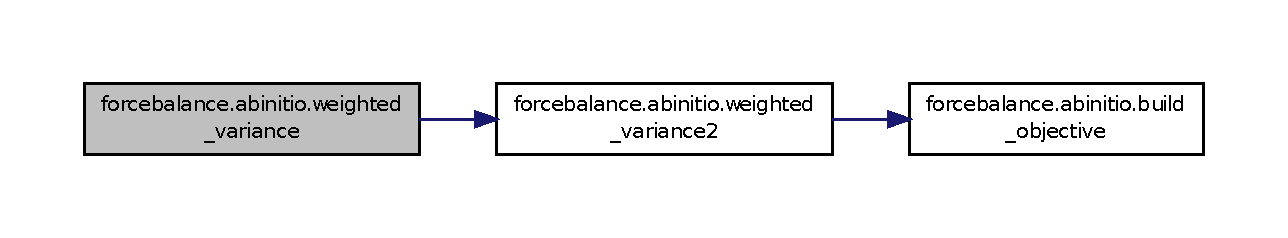
\includegraphics[width=350pt]{namespaceforcebalance_1_1abinitio_aba970cb59bab95eec79027ea05655110_cgraph}
\end{center}
\end{figure}


\hypertarget{namespaceforcebalance_1_1abinitio_ab9554761125a4ec7c3c13d6ae4ea537d}{\index{forcebalance\-::abinitio@{forcebalance\-::abinitio}!weighted\-\_\-variance2@{weighted\-\_\-variance2}}
\index{weighted\-\_\-variance2@{weighted\-\_\-variance2}!forcebalance::abinitio@{forcebalance\-::abinitio}}
\paragraph[{weighted\-\_\-variance2}]{\setlength{\rightskip}{0pt plus 5cm}def forcebalance.\-abinitio.\-weighted\-\_\-variance2 (
\begin{DoxyParamCaption}
\item[{}]{S\-Pi\-Xi, }
\item[{}]{W\-Ci\-W, }
\item[{}]{Z, }
\item[{}]{L, }
\item[{}]{R, }
\item[{}]{L2, }
\item[{}]{R2, }
\item[{}]{N\-C\-P1, }
\item[{}]{subtract\-\_\-mean = {\ttfamily True}}
\end{DoxyParamCaption}
)}}\label{namespaceforcebalance_1_1abinitio_ab9554761125a4ec7c3c13d6ae4ea537d}


A bit of a hack, since we have to subtract out two mean quantities to get Hessian elements. 



Definition at line 1135 of file abinitio.\-py.



Here is the call graph for this function\-:
\nopagebreak
\begin{figure}[H]
\begin{center}
\leavevmode
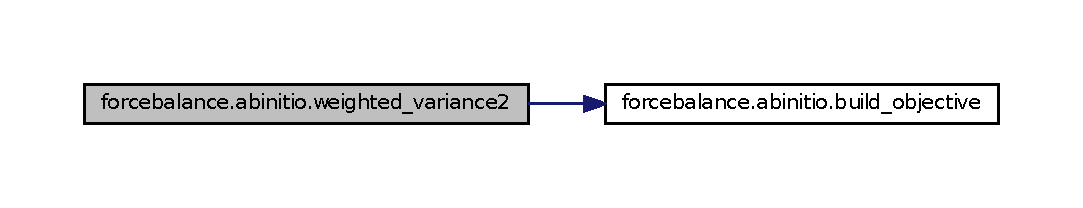
\includegraphics[width=350pt]{namespaceforcebalance_1_1abinitio_ab9554761125a4ec7c3c13d6ae4ea537d_cgraph}
\end{center}
\end{figure}



\hypertarget{namespaceforcebalance_1_1abinitio__internal}{\subsection{forcebalance.\-abinitio\-\_\-internal Namespace Reference}
\label{namespaceforcebalance_1_1abinitio__internal}\index{forcebalance.\-abinitio\-\_\-internal@{forcebalance.\-abinitio\-\_\-internal}}
}


Internal implementation of energy matching (for T\-I\-P3\-P water only)  


\subsubsection*{Classes}
\begin{DoxyCompactItemize}
\item 
class \hyperlink{classforcebalance_1_1abinitio__internal_1_1AbInitio__Internal}{Ab\-Initio\-\_\-\-Internal}
\begin{DoxyCompactList}\small\item\em Subclass of Target for force and energy matching using an internal implementation. \end{DoxyCompactList}\end{DoxyCompactItemize}


\subsubsection{Detailed Description}
Internal implementation of energy matching (for T\-I\-P3\-P water only) \begin{DoxyAuthor}{Author}
Lee-\/\-Ping Wang 
\end{DoxyAuthor}
\begin{DoxyDate}{Date}
04/2012 
\end{DoxyDate}

\hypertarget{namespaceforcebalance_1_1amberio}{\subsection{forcebalance\-:\-:amberio \-Namespace \-Reference}
\label{namespaceforcebalance_1_1amberio}\index{forcebalance\-::amberio@{forcebalance\-::amberio}}
}


\-A\-M\-B\-E\-R force field input/output.  


\subsubsection*{\-Classes}
\begin{DoxyCompactItemize}
\item 
class \hyperlink{classforcebalance_1_1amberio_1_1Mol2__Reader}{\-Mol2\-\_\-\-Reader}
\begin{DoxyCompactList}\small\item\em \-Finite state machine for parsing \hyperlink{namespaceforcebalance_1_1Mol2}{\-Mol2} force field file. \end{DoxyCompactList}\item 
class \hyperlink{classforcebalance_1_1amberio_1_1FrcMod__Reader}{\-Frc\-Mod\-\_\-\-Reader}
\begin{DoxyCompactList}\small\item\em \-Finite state machine for parsing \-Frc\-Mod force field file. \end{DoxyCompactList}\item 
class \hyperlink{classforcebalance_1_1amberio_1_1AbInitio__AMBER}{\-Ab\-Initio\-\_\-\-A\-M\-B\-E\-R}
\begin{DoxyCompactList}\small\item\em \-Subclass of \-Target for force and energy matching using \-A\-M\-B\-E\-R. \end{DoxyCompactList}\end{DoxyCompactItemize}
\subsubsection*{\-Functions}
\begin{DoxyCompactItemize}
\item 
def \hyperlink{namespaceforcebalance_1_1amberio_af59589a24e815a11db69dcaa21c51659}{is\-\_\-mol2\-\_\-atom}
\end{DoxyCompactItemize}
\subsubsection*{\-Variables}
\begin{DoxyCompactItemize}
\item 
tuple \hyperlink{namespaceforcebalance_1_1amberio_aa9ff86ae6726b8e8fc8b27ddf29e095a}{logger} = get\-Logger(\-\_\-\-\_\-name\-\_\-\-\_\-)
\item 
dictionary \hyperlink{namespaceforcebalance_1_1amberio_a7b3741ff909d0776c26574cfee9807fd}{mol2\-\_\-pdict} = \{'\-C\-O\-U\-L'\-:\{'\-Atom'\-:\mbox{[}1\mbox{]}, 8\-:''\}\}
\item 
dictionary \hyperlink{namespaceforcebalance_1_1amberio_ae5ba6128e5e02a120e8bcd688a5b1be4}{frcmod\-\_\-pdict}
\end{DoxyCompactItemize}


\subsubsection{\-Detailed \-Description}
\-A\-M\-B\-E\-R force field input/output. \-This serves as a good template for writing future force matching \-I/\-O modules for other programs because it's so simple.

\begin{DoxyAuthor}{\-Author}
\-Lee-\/\-Ping \-Wang 
\end{DoxyAuthor}
\begin{DoxyDate}{\-Date}
01/2012 
\end{DoxyDate}


\subsubsection{\-Function \-Documentation}
\hypertarget{namespaceforcebalance_1_1amberio_af59589a24e815a11db69dcaa21c51659}{\index{forcebalance\-::amberio@{forcebalance\-::amberio}!is\-\_\-mol2\-\_\-atom@{is\-\_\-mol2\-\_\-atom}}
\index{is\-\_\-mol2\-\_\-atom@{is\-\_\-mol2\-\_\-atom}!forcebalance::amberio@{forcebalance\-::amberio}}
\paragraph[{is\-\_\-mol2\-\_\-atom}]{\setlength{\rightskip}{0pt plus 5cm}def {\bf forcebalance.\-amberio.\-is\-\_\-mol2\-\_\-atom} (
\begin{DoxyParamCaption}
\item[{}]{line}
\end{DoxyParamCaption}
)}}\label{namespaceforcebalance_1_1amberio_af59589a24e815a11db69dcaa21c51659}


\-Definition at line 35 of file amberio.\-py.



\-Here is the call graph for this function\-:\nopagebreak
\begin{figure}[H]
\begin{center}
\leavevmode
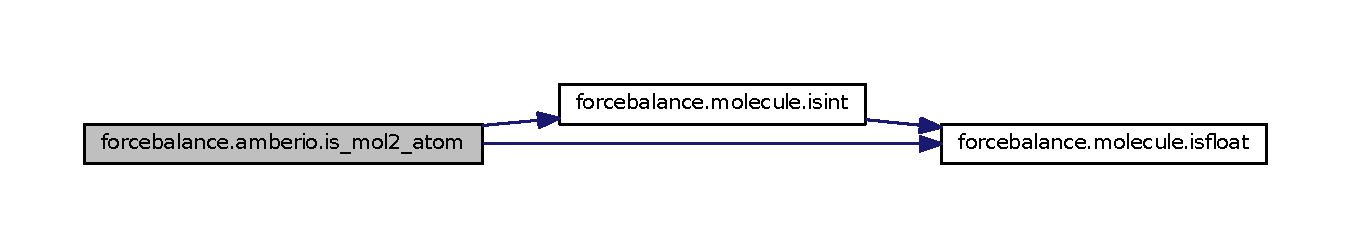
\includegraphics[width=350pt]{namespaceforcebalance_1_1amberio_af59589a24e815a11db69dcaa21c51659_cgraph}
\end{center}
\end{figure}




\subsubsection{\-Variable \-Documentation}
\hypertarget{namespaceforcebalance_1_1amberio_ae5ba6128e5e02a120e8bcd688a5b1be4}{\index{forcebalance\-::amberio@{forcebalance\-::amberio}!frcmod\-\_\-pdict@{frcmod\-\_\-pdict}}
\index{frcmod\-\_\-pdict@{frcmod\-\_\-pdict}!forcebalance::amberio@{forcebalance\-::amberio}}
\paragraph[{frcmod\-\_\-pdict}]{\setlength{\rightskip}{0pt plus 5cm}dictionary {\bf forcebalance\-::amberio\-::frcmod\-\_\-pdict}}}\label{namespaceforcebalance_1_1amberio_ae5ba6128e5e02a120e8bcd688a5b1be4}
{\bfseries \-Initial value\-:}
\begin{DoxyCode}
1 {'BONDS': {'Atom':[0], 1:'K', 2:'B'},
2                 'ANGLES':{'Atom':[0], 1:'K', 2:'B'},
3                 'PDIHS1':{'Atom':[0], 2:'K', 3:'B'},
4                 'PDIHS2':{'Atom':[0], 2:'K', 3:'B'},
5                 'PDIHS3':{'Atom':[0], 2:'K', 3:'B'},
6                 'PDIHS4':{'Atom':[0], 2:'K', 3:'B'},
7                 'PDIHS5':{'Atom':[0], 2:'K', 3:'B'},
8                 'PDIHS6':{'Atom':[0], 2:'K', 3:'B'},
9                 'IDIHS' :{'Atom':[0], 1:'K', 3:'B'},
10                 'VDW':{'Atom':[0], 1:'S', 2:'T'}
11                 }
\end{DoxyCode}


\-Definition at line 23 of file amberio.\-py.

\hypertarget{namespaceforcebalance_1_1amberio_aa9ff86ae6726b8e8fc8b27ddf29e095a}{\index{forcebalance\-::amberio@{forcebalance\-::amberio}!logger@{logger}}
\index{logger@{logger}!forcebalance::amberio@{forcebalance\-::amberio}}
\paragraph[{logger}]{\setlength{\rightskip}{0pt plus 5cm}tuple {\bf forcebalance\-::amberio\-::logger} = get\-Logger(\-\_\-\-\_\-name\-\_\-\-\_\-)}}\label{namespaceforcebalance_1_1amberio_aa9ff86ae6726b8e8fc8b27ddf29e095a}


\-Definition at line 19 of file amberio.\-py.

\hypertarget{namespaceforcebalance_1_1amberio_a7b3741ff909d0776c26574cfee9807fd}{\index{forcebalance\-::amberio@{forcebalance\-::amberio}!mol2\-\_\-pdict@{mol2\-\_\-pdict}}
\index{mol2\-\_\-pdict@{mol2\-\_\-pdict}!forcebalance::amberio@{forcebalance\-::amberio}}
\paragraph[{mol2\-\_\-pdict}]{\setlength{\rightskip}{0pt plus 5cm}dictionary {\bf forcebalance\-::amberio\-::mol2\-\_\-pdict} = \{'\-C\-O\-U\-L'\-:\{'\-Atom'\-:\mbox{[}1\mbox{]}, 8\-:''\}\}}}\label{namespaceforcebalance_1_1amberio_a7b3741ff909d0776c26574cfee9807fd}


\-Definition at line 21 of file amberio.\-py.


\hypertarget{namespaceforcebalance_1_1binding}{\subsection{forcebalance.\-binding Namespace Reference}
\label{namespaceforcebalance_1_1binding}\index{forcebalance.\-binding@{forcebalance.\-binding}}
}


Binding energy fitting module.  


\subsubsection*{Classes}
\begin{DoxyCompactItemize}
\item 
class \hyperlink{classforcebalance_1_1binding_1_1BindingEnergy}{Binding\-Energy}
\begin{DoxyCompactList}\small\item\em Improved subclass of Target for fitting force fields to binding energies. \end{DoxyCompactList}\end{DoxyCompactItemize}
\subsubsection*{Functions}
\begin{DoxyCompactItemize}
\item 
def \hyperlink{namespaceforcebalance_1_1binding_a0ae2f9f7a4ab7f4c64f8826de52331e9}{parse\-\_\-interactions}
\begin{DoxyCompactList}\small\item\em Parse through the interactions input file. \end{DoxyCompactList}\end{DoxyCompactItemize}
\subsubsection*{Variables}
\begin{DoxyCompactItemize}
\item 
tuple \hyperlink{namespaceforcebalance_1_1binding_a0bdb0d0390122623a60dae0e08bdc84a}{logger} = get\-Logger(\-\_\-\-\_\-name\-\_\-\-\_\-)
\end{DoxyCompactItemize}


\subsubsection{Detailed Description}
Binding energy fitting module. \begin{DoxyAuthor}{Author}
Lee-\/\-Ping Wang 
\end{DoxyAuthor}
\begin{DoxyDate}{Date}
05/2012 
\end{DoxyDate}


\subsubsection{Function Documentation}
\hypertarget{namespaceforcebalance_1_1binding_a0ae2f9f7a4ab7f4c64f8826de52331e9}{\index{forcebalance\-::binding@{forcebalance\-::binding}!parse\-\_\-interactions@{parse\-\_\-interactions}}
\index{parse\-\_\-interactions@{parse\-\_\-interactions}!forcebalance::binding@{forcebalance\-::binding}}
\paragraph[{parse\-\_\-interactions}]{\setlength{\rightskip}{0pt plus 5cm}def forcebalance.\-binding.\-parse\-\_\-interactions (
\begin{DoxyParamCaption}
\item[{}]{input\-\_\-file}
\end{DoxyParamCaption}
)}}\label{namespaceforcebalance_1_1binding_a0ae2f9f7a4ab7f4c64f8826de52331e9}


Parse through the interactions input file. 


\begin{DoxyParams}[1]{Parameters}
\mbox{\tt in}  & {\em input\-\_\-file} & The name of the input file. \\
\hline
\end{DoxyParams}


Definition at line 33 of file binding.\-py.



Here is the call graph for this function\-:\nopagebreak
\begin{figure}[H]
\begin{center}
\leavevmode
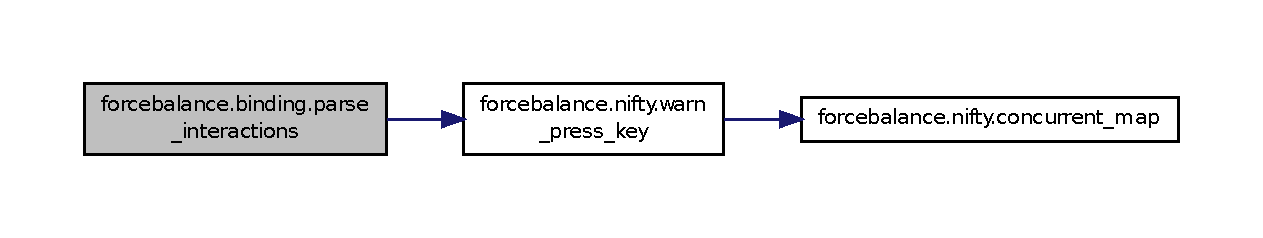
\includegraphics[width=350pt]{namespaceforcebalance_1_1binding_a0ae2f9f7a4ab7f4c64f8826de52331e9_cgraph}
\end{center}
\end{figure}




\subsubsection{Variable Documentation}
\hypertarget{namespaceforcebalance_1_1binding_a0bdb0d0390122623a60dae0e08bdc84a}{\index{forcebalance\-::binding@{forcebalance\-::binding}!logger@{logger}}
\index{logger@{logger}!forcebalance::binding@{forcebalance\-::binding}}
\paragraph[{logger}]{\setlength{\rightskip}{0pt plus 5cm}tuple forcebalance.\-binding.\-logger = get\-Logger(\-\_\-\-\_\-name\-\_\-\-\_\-)}}\label{namespaceforcebalance_1_1binding_a0bdb0d0390122623a60dae0e08bdc84a}


Definition at line 22 of file binding.\-py.


\hypertarget{namespaceforcebalance_1_1chemistry}{\subsection{forcebalance.\-chemistry Namespace Reference}
\label{namespaceforcebalance_1_1chemistry}\index{forcebalance.\-chemistry@{forcebalance.\-chemistry}}
}

\hypertarget{namespaceforcebalance_1_1contact}{\subsection{forcebalance\-:\-:contact \-Namespace \-Reference}
\label{namespaceforcebalance_1_1contact}\index{forcebalance\-::contact@{forcebalance\-::contact}}
}
\subsubsection*{\-Functions}
\begin{DoxyCompactItemize}
\item 
def \hyperlink{namespaceforcebalance_1_1contact_a3592dbbf524c6115f34d9a70b50e2e0f}{atom\-\_\-distances}
\begin{DoxyCompactList}\small\item\em \-For each frame in xyzlist, compute the (euclidean) distance between pairs of atoms whos indices are given in contacts. \end{DoxyCompactList}\item 
def \hyperlink{namespaceforcebalance_1_1contact_acffb04a66580454b8a87648faa1c5c16}{residue\-\_\-distances}
\begin{DoxyCompactList}\small\item\em \-For each frame in xyzlist, and for each pair of residues in the array contact, compute the distance between the closest pair of atoms such that one of them belongs to each residue. \end{DoxyCompactList}\end{DoxyCompactItemize}


\subsubsection{\-Function \-Documentation}
\hypertarget{namespaceforcebalance_1_1contact_a3592dbbf524c6115f34d9a70b50e2e0f}{\index{forcebalance\-::contact@{forcebalance\-::contact}!atom\-\_\-distances@{atom\-\_\-distances}}
\index{atom\-\_\-distances@{atom\-\_\-distances}!forcebalance::contact@{forcebalance\-::contact}}
\paragraph[{atom\-\_\-distances}]{\setlength{\rightskip}{0pt plus 5cm}def {\bf forcebalance.\-contact.\-atom\-\_\-distances} (
\begin{DoxyParamCaption}
\item[{}]{xyzlist, }
\item[{}]{atom\-\_\-contacts}
\end{DoxyParamCaption}
)}}\label{namespaceforcebalance_1_1contact_a3592dbbf524c6115f34d9a70b50e2e0f}


\-For each frame in xyzlist, compute the (euclidean) distance between pairs of atoms whos indices are given in contacts. 

xyzlist should be a traj\-\_\-length x num\-\_\-atoms x num\-\_\-dims array of type float32

contacts should be a num\-\_\-contacts x 2 array where each row gives the indices of 2 atoms whos distance you care to monitor.

\-Returns\-: traj\-\_\-length x num\-\_\-contacts array of euclidean distances

\-Note\-: \-For nice wrappers around this, see the prepare\-\_\-trajectory method of various metrics in metrics.\-py 

\-Definition at line 26 of file contact.\-py.



\-Here is the call graph for this function\-:\nopagebreak
\begin{figure}[H]
\begin{center}
\leavevmode
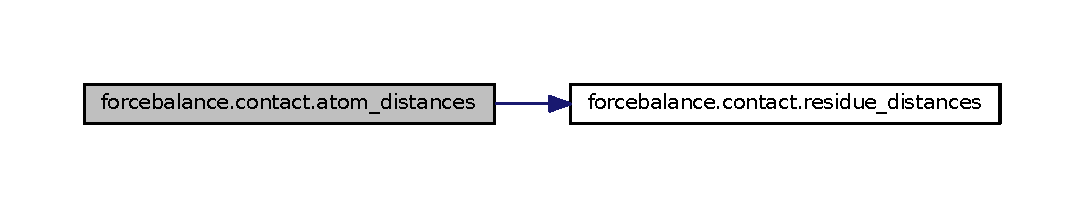
\includegraphics[width=350pt]{namespaceforcebalance_1_1contact_a3592dbbf524c6115f34d9a70b50e2e0f_cgraph}
\end{center}
\end{figure}


\hypertarget{namespaceforcebalance_1_1contact_acffb04a66580454b8a87648faa1c5c16}{\index{forcebalance\-::contact@{forcebalance\-::contact}!residue\-\_\-distances@{residue\-\_\-distances}}
\index{residue\-\_\-distances@{residue\-\_\-distances}!forcebalance::contact@{forcebalance\-::contact}}
\paragraph[{residue\-\_\-distances}]{\setlength{\rightskip}{0pt plus 5cm}def {\bf forcebalance.\-contact.\-residue\-\_\-distances} (
\begin{DoxyParamCaption}
\item[{}]{xyzlist, }
\item[{}]{residue\-\_\-membership, }
\item[{}]{residue\-\_\-contacts}
\end{DoxyParamCaption}
)}}\label{namespaceforcebalance_1_1contact_acffb04a66580454b8a87648faa1c5c16}


\-For each frame in xyzlist, and for each pair of residues in the array contact, compute the distance between the closest pair of atoms such that one of them belongs to each residue. 

xyzlist should be a traj\-\_\-length x num\-\_\-atoms x num\-\_\-dims array of type float32

residue\-\_\-membership should be a list of lists where residue\-\_\-membership\mbox{[}i\mbox{]} gives the list of atomindices that belong to residue i. residue\-\_\-membership should \-N\-O\-T be a numpy 2\-D array unless you really mean that all of the residues have the same number of atoms

residue\-\_\-contacts should be a 2\-D numpy array of shape num\-\_\-contacts x 2 where each row gives the indices of the two \-R\-E\-S\-I\-D\-U\-E\-S who you are interested in monitoring for a contact.

\-Returns\-: a 2\-D array of traj\-\_\-lenth x num\-\_\-contacts where out\mbox{[}i,j\mbox{]} contains the distance between the pair of atoms, one from residue\-\_\-membership\mbox{[}residue\-\_\-contacts\mbox{[}j,0\mbox{]}\mbox{]} and one from residue\-\_\-membership\mbox{[}residue\-\_\-contacts\mbox{[}j,1\mbox{]}\mbox{]} that are closest. 

\-Definition at line 85 of file contact.\-py.


\hypertarget{namespaceforcebalance_1_1counterpoise}{\subsection{forcebalance.\-counterpoise Namespace Reference}
\label{namespaceforcebalance_1_1counterpoise}\index{forcebalance.\-counterpoise@{forcebalance.\-counterpoise}}
}


Match an empirical potential to the counterpoise correction for basis set superposition error (B\-S\-S\-E).  


\subsubsection*{Classes}
\begin{DoxyCompactItemize}
\item 
class \hyperlink{classforcebalance_1_1counterpoise_1_1Counterpoise}{Counterpoise}
\begin{DoxyCompactList}\small\item\em Target subclass for matching the counterpoise correction. \end{DoxyCompactList}\end{DoxyCompactItemize}
\subsubsection*{Variables}
\begin{DoxyCompactItemize}
\item 
tuple \hyperlink{namespaceforcebalance_1_1counterpoise_a9a7008a650c37185e7e43c9b1c943bd6}{logger} = get\-Logger(\-\_\-\-\_\-name\-\_\-\-\_\-)
\end{DoxyCompactItemize}


\subsubsection{Detailed Description}
Match an empirical potential to the counterpoise correction for basis set superposition error (B\-S\-S\-E). Here we test two different functional forms\-: a three-\/parameter Gaussian repulsive potential and a four-\/parameter Gaussian which goes smoothly to an exponential. The latter can be written in two different ways -\/ one which gives us control over the exponential, the switching distance and the Gaussian decay constant, and another which gives us control over the Gaussian and the switching distance. They are called 'C\-P\-G\-A\-U\-S\-S', 'C\-P\-E\-X\-P\-G', and 'C\-P\-G\-E\-X\-P'. I think the third option is the best although our early tests have indicated that none of the force fields perform particularly well for the water dimer.

This subclass of Target implements the 'get' method.

\begin{DoxyAuthor}{Author}
Lee-\/\-Ping Wang 
\end{DoxyAuthor}
\begin{DoxyDate}{Date}
12/2011 
\end{DoxyDate}


\subsubsection{Variable Documentation}
\hypertarget{namespaceforcebalance_1_1counterpoise_a9a7008a650c37185e7e43c9b1c943bd6}{\index{forcebalance\-::counterpoise@{forcebalance\-::counterpoise}!logger@{logger}}
\index{logger@{logger}!forcebalance::counterpoise@{forcebalance\-::counterpoise}}
\paragraph[{logger}]{\setlength{\rightskip}{0pt plus 5cm}tuple forcebalance.\-counterpoise.\-logger = get\-Logger(\-\_\-\-\_\-name\-\_\-\-\_\-)}}\label{namespaceforcebalance_1_1counterpoise_a9a7008a650c37185e7e43c9b1c943bd6}


Definition at line 29 of file counterpoise.\-py.


\hypertarget{namespaceforcebalance_1_1custom__io}{\subsection{forcebalance\-:\-:custom\-\_\-io \-Namespace \-Reference}
\label{namespaceforcebalance_1_1custom__io}\index{forcebalance\-::custom\-\_\-io@{forcebalance\-::custom\-\_\-io}}
}


\-Custom force field parser.  


\subsubsection*{\-Classes}
\begin{DoxyCompactItemize}
\item 
class \hyperlink{classforcebalance_1_1custom__io_1_1Gen__Reader}{\-Gen\-\_\-\-Reader}
\begin{DoxyCompactList}\small\item\em \-Finite state machine for parsing custom \-G\-R\-O\-M\-A\-C\-S force field files. \end{DoxyCompactList}\end{DoxyCompactItemize}
\subsubsection*{\-Variables}
\begin{DoxyCompactItemize}
\item 
list \hyperlink{namespaceforcebalance_1_1custom__io_a509d4c2b5eeee4278adde414e55eb560}{cptypes} = \mbox{[}\-None, '\-C\-P\-G\-A\-U\-S\-S', '\-C\-P\-E\-X\-P\-G', '\-C\-P\-G\-E\-X\-P'\mbox{]}
\begin{DoxyCompactList}\small\item\em \-Types of counterpoise correction. \end{DoxyCompactList}\item 
list \hyperlink{namespaceforcebalance_1_1custom__io_a604fd5cd1f0c6057a8a72ac61b55f6fa}{ndtypes} = \mbox{[}\-None\mbox{]}
\begin{DoxyCompactList}\small\item\em \-Types of \-N\-D\-D\-O correction. \end{DoxyCompactList}\item 
dictionary \hyperlink{namespaceforcebalance_1_1custom__io_a64c7f292c64ad2b2b855a82e68c0ca7e}{fdict}
\begin{DoxyCompactList}\small\item\em \-Section -\/$>$ \-Interaction type dictionary. \end{DoxyCompactList}\item 
dictionary \hyperlink{namespaceforcebalance_1_1custom__io_aaa87b8099dee5dfec42f5869dabad0c5}{pdict}
\begin{DoxyCompactList}\small\item\em \-Interaction type -\/$>$ \-Parameter \-Dictionary. \end{DoxyCompactList}\end{DoxyCompactItemize}


\subsubsection{\-Detailed \-Description}
\-Custom force field parser. \-We take advantage of the sections in \-G\-R\-O\-M\-A\-C\-S and the 'interaction type' concept, but these interactions are not supported in \-G\-R\-O\-M\-A\-C\-S; rather, they are computed within our program.

\begin{DoxyAuthor}{\-Author}
\-Lee-\/\-Ping \-Wang 
\end{DoxyAuthor}
\begin{DoxyDate}{\-Date}
12/2011 
\end{DoxyDate}


\subsubsection{\-Variable \-Documentation}
\hypertarget{namespaceforcebalance_1_1custom__io_a509d4c2b5eeee4278adde414e55eb560}{\index{forcebalance\-::custom\-\_\-io@{forcebalance\-::custom\-\_\-io}!cptypes@{cptypes}}
\index{cptypes@{cptypes}!forcebalance::custom_io@{forcebalance\-::custom\-\_\-io}}
\paragraph[{cptypes}]{\setlength{\rightskip}{0pt plus 5cm}list {\bf forcebalance\-::custom\-\_\-io\-::cptypes} = \mbox{[}\-None, '\-C\-P\-G\-A\-U\-S\-S', '\-C\-P\-E\-X\-P\-G', '\-C\-P\-G\-E\-X\-P'\mbox{]}}}\label{namespaceforcebalance_1_1custom__io_a509d4c2b5eeee4278adde414e55eb560}


\-Types of counterpoise correction. 



\-Definition at line 16 of file custom\-\_\-io.\-py.

\hypertarget{namespaceforcebalance_1_1custom__io_a64c7f292c64ad2b2b855a82e68c0ca7e}{\index{forcebalance\-::custom\-\_\-io@{forcebalance\-::custom\-\_\-io}!fdict@{fdict}}
\index{fdict@{fdict}!forcebalance::custom_io@{forcebalance\-::custom\-\_\-io}}
\paragraph[{fdict}]{\setlength{\rightskip}{0pt plus 5cm}dictionary {\bf forcebalance\-::custom\-\_\-io\-::fdict}}}\label{namespaceforcebalance_1_1custom__io_a64c7f292c64ad2b2b855a82e68c0ca7e}
{\bfseries \-Initial value\-:}
\begin{DoxyCode}
1 {
2     'counterpoise'  : cptypes    }
\end{DoxyCode}


\-Section -\/$>$ \-Interaction type dictionary. 



\-Definition at line 21 of file custom\-\_\-io.\-py.

\hypertarget{namespaceforcebalance_1_1custom__io_a604fd5cd1f0c6057a8a72ac61b55f6fa}{\index{forcebalance\-::custom\-\_\-io@{forcebalance\-::custom\-\_\-io}!ndtypes@{ndtypes}}
\index{ndtypes@{ndtypes}!forcebalance::custom_io@{forcebalance\-::custom\-\_\-io}}
\paragraph[{ndtypes}]{\setlength{\rightskip}{0pt plus 5cm}list {\bf forcebalance\-::custom\-\_\-io\-::ndtypes} = \mbox{[}\-None\mbox{]}}}\label{namespaceforcebalance_1_1custom__io_a604fd5cd1f0c6057a8a72ac61b55f6fa}


\-Types of \-N\-D\-D\-O correction. 



\-Definition at line 18 of file custom\-\_\-io.\-py.

\hypertarget{namespaceforcebalance_1_1custom__io_aaa87b8099dee5dfec42f5869dabad0c5}{\index{forcebalance\-::custom\-\_\-io@{forcebalance\-::custom\-\_\-io}!pdict@{pdict}}
\index{pdict@{pdict}!forcebalance::custom_io@{forcebalance\-::custom\-\_\-io}}
\paragraph[{pdict}]{\setlength{\rightskip}{0pt plus 5cm}dictionary {\bf forcebalance\-::custom\-\_\-io\-::pdict}}}\label{namespaceforcebalance_1_1custom__io_aaa87b8099dee5dfec42f5869dabad0c5}
{\bfseries \-Initial value\-:}
\begin{DoxyCode}
1 {'CPGAUSS':{3:'A', 4:'B', 5:'C'},
2          'CPGEXP' :{3:'A', 4:'B', 5:'G', 6:'X'},
3          'CPEXPG' :{3:'A1', 4:'B', 5:'X0', 6:'A2'}
4          }
\end{DoxyCode}


\-Interaction type -\/$>$ \-Parameter \-Dictionary. 



\-Definition at line 25 of file custom\-\_\-io.\-py.


\hypertarget{namespaceforcebalance_1_1engine}{\subsection{forcebalance\-:\-:engine \-Namespace \-Reference}
\label{namespaceforcebalance_1_1engine}\index{forcebalance\-::engine@{forcebalance\-::engine}}
}
\subsubsection*{\-Classes}
\begin{DoxyCompactItemize}
\item 
class \hyperlink{classforcebalance_1_1engine_1_1Engine}{\-Engine}
\begin{DoxyCompactList}\small\item\em \-Base class for all engines. \end{DoxyCompactList}\end{DoxyCompactItemize}
\subsubsection*{\-Variables}
\begin{DoxyCompactItemize}
\item 
tuple \hyperlink{namespaceforcebalance_1_1engine_ae4a289a63d0f20258665d7c5208cf2a2}{logger} = get\-Logger(\-\_\-\-\_\-name\-\_\-\-\_\-)
\end{DoxyCompactItemize}


\subsubsection{\-Variable \-Documentation}
\hypertarget{namespaceforcebalance_1_1engine_ae4a289a63d0f20258665d7c5208cf2a2}{\index{forcebalance\-::engine@{forcebalance\-::engine}!logger@{logger}}
\index{logger@{logger}!forcebalance::engine@{forcebalance\-::engine}}
\paragraph[{logger}]{\setlength{\rightskip}{0pt plus 5cm}tuple {\bf forcebalance\-::engine\-::logger} = get\-Logger(\-\_\-\-\_\-name\-\_\-\-\_\-)}}\label{namespaceforcebalance_1_1engine_ae4a289a63d0f20258665d7c5208cf2a2}


\-Definition at line 17 of file engine.\-py.


\hypertarget{namespaceforcebalance_1_1finite__difference}{\subsection{forcebalance.\-finite\-\_\-difference Namespace Reference}
\label{namespaceforcebalance_1_1finite__difference}\index{forcebalance.\-finite\-\_\-difference@{forcebalance.\-finite\-\_\-difference}}
}
\subsubsection*{Functions}
\begin{DoxyCompactItemize}
\item 
def \hyperlink{namespaceforcebalance_1_1finite__difference_ac5bb1552a9b8dd22c9c80e6444de2218}{f1d2p}
\begin{DoxyCompactList}\small\item\em A two-\/point finite difference stencil. \end{DoxyCompactList}\item 
def \hyperlink{namespaceforcebalance_1_1finite__difference_a123c5d5dea0f3f50ab57796bb3bc39be}{f1d5p}
\begin{DoxyCompactList}\small\item\em A highly accurate five-\/point finite difference stencil for computing derivatives of a function. \end{DoxyCompactList}\item 
def \hyperlink{namespaceforcebalance_1_1finite__difference_a9be9f0d21300958092e380514e2e980d}{f1d7p}
\begin{DoxyCompactList}\small\item\em A highly accurate seven-\/point finite difference stencil for computing derivatives of a function. \end{DoxyCompactList}\item 
def \hyperlink{namespaceforcebalance_1_1finite__difference_acc281f85b668062745f711d9b4a610fa}{f12d7p}
\item 
def \hyperlink{namespaceforcebalance_1_1finite__difference_aa69a8819e4680091f400303c1d6ddeb7}{f12d3p}
\begin{DoxyCompactList}\small\item\em A three-\/point finite difference stencil. \end{DoxyCompactList}\item 
def \hyperlink{namespaceforcebalance_1_1finite__difference_ad84d3e385db1190e7d8ef58bc08a6c52}{in\-\_\-fd}
\begin{DoxyCompactList}\small\item\em Invoking this function from anywhere will tell us whether we're being called by a finite-\/difference function. \end{DoxyCompactList}\item 
def \hyperlink{namespaceforcebalance_1_1finite__difference_ae484c591ae8c4e5bae73a0ef2660c339}{fdwrap}
\begin{DoxyCompactList}\small\item\em A function wrapper for finite difference designed for differentiating 'get'-\/type functions. \end{DoxyCompactList}\item 
def \hyperlink{namespaceforcebalance_1_1finite__difference_a00322fb65860c390616f74d05037c797}{fdwrap\-\_\-\-G}
\begin{DoxyCompactList}\small\item\em A driver to fdwrap for gradients (see documentation for fdwrap) Inputs\-: tgt = The Target containing the objective function that we want to differentiate mvals0 = The 'central' values of the mathematical parameters -\/ i.\-e. \end{DoxyCompactList}\item 
def \hyperlink{namespaceforcebalance_1_1finite__difference_a77a0bc1ae3cbbcc8d38a0ef9ca877d6d}{fdwrap\-\_\-\-H}
\begin{DoxyCompactList}\small\item\em A driver to fdwrap for Hessians (see documentation for fdwrap) Inputs\-: tgt = The Target containing the objective function that we want to differentiate mvals0 = The 'central' values of the mathematical parameters -\/ i.\-e. \end{DoxyCompactList}\end{DoxyCompactItemize}
\subsubsection*{Variables}
\begin{DoxyCompactItemize}
\item 
tuple \hyperlink{namespaceforcebalance_1_1finite__difference_a2bdf74505c45f442e1c96d557414254e}{logger} = get\-Logger(\-\_\-\-\_\-name\-\_\-\-\_\-)
\end{DoxyCompactItemize}


\subsubsection{Function Documentation}
\hypertarget{namespaceforcebalance_1_1finite__difference_aa69a8819e4680091f400303c1d6ddeb7}{\index{forcebalance\-::finite\-\_\-difference@{forcebalance\-::finite\-\_\-difference}!f12d3p@{f12d3p}}
\index{f12d3p@{f12d3p}!forcebalance::finite_difference@{forcebalance\-::finite\-\_\-difference}}
\paragraph[{f12d3p}]{\setlength{\rightskip}{0pt plus 5cm}def forcebalance.\-finite\-\_\-difference.\-f12d3p (
\begin{DoxyParamCaption}
\item[{}]{f, }
\item[{}]{h, }
\item[{}]{f0 = {\ttfamily None}}
\end{DoxyParamCaption}
)}}\label{namespaceforcebalance_1_1finite__difference_aa69a8819e4680091f400303c1d6ddeb7}


A three-\/point finite difference stencil. 

This function does either two computations or three, depending on whether the 'center' value is supplied. This is done in order to avoid recomputing the center value many times.

The first derivative is evaluated using central difference. One advantage of using central difference (as opposed to forward difference) is that we get zero at the bottom of a parabola.

Using this formula we also get an approximate second derivative, which can then be inserted into the diagonal of the Hessian. This is very useful for optimizations like B\-F\-G\-S where the diagonal determines how far we step in the parameter space.

How to use\-: use fdwrap or something similar to generate a one-\/variable function from the (usually) much more complicated function that we wish to differentate. Then pass it to this function.

Inputs\-: f = The one-\/variable function f(x) that we're differentiating h = The finite difference step size, usually a small number

Outputs\-: fp = The finite difference derivative of the function f(x) around x=0. 

Definition at line 109 of file finite\-\_\-difference.\-py.



Here is the call graph for this function\-:\nopagebreak
\begin{figure}[H]
\begin{center}
\leavevmode
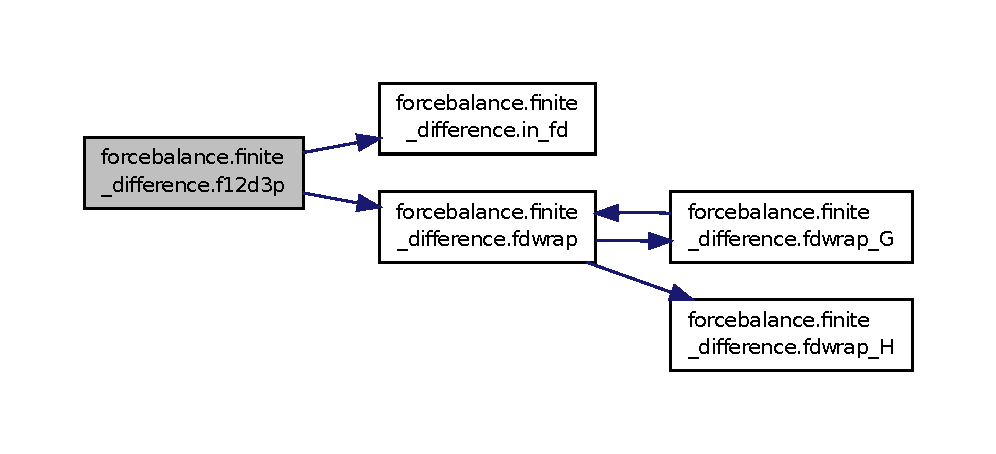
\includegraphics[width=350pt]{namespaceforcebalance_1_1finite__difference_aa69a8819e4680091f400303c1d6ddeb7_cgraph}
\end{center}
\end{figure}


\hypertarget{namespaceforcebalance_1_1finite__difference_acc281f85b668062745f711d9b4a610fa}{\index{forcebalance\-::finite\-\_\-difference@{forcebalance\-::finite\-\_\-difference}!f12d7p@{f12d7p}}
\index{f12d7p@{f12d7p}!forcebalance::finite_difference@{forcebalance\-::finite\-\_\-difference}}
\paragraph[{f12d7p}]{\setlength{\rightskip}{0pt plus 5cm}def forcebalance.\-finite\-\_\-difference.\-f12d7p (
\begin{DoxyParamCaption}
\item[{}]{f, }
\item[{}]{h}
\end{DoxyParamCaption}
)}}\label{namespaceforcebalance_1_1finite__difference_acc281f85b668062745f711d9b4a610fa}


Definition at line 75 of file finite\-\_\-difference.\-py.



Here is the call graph for this function\-:\nopagebreak
\begin{figure}[H]
\begin{center}
\leavevmode
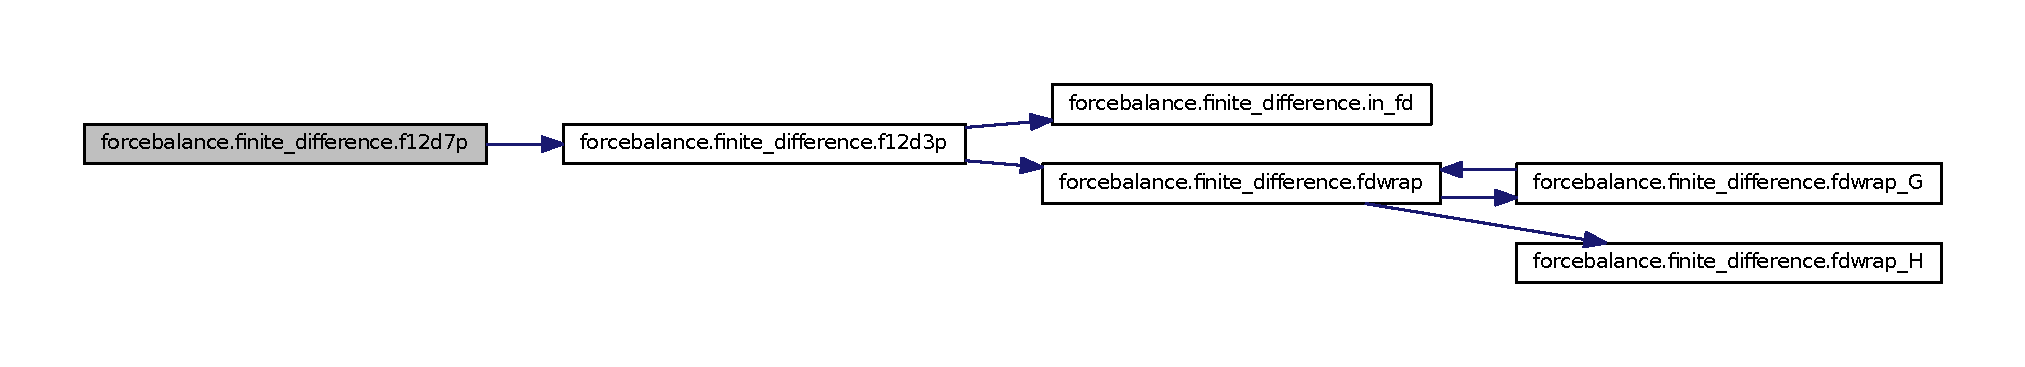
\includegraphics[width=350pt]{namespaceforcebalance_1_1finite__difference_acc281f85b668062745f711d9b4a610fa_cgraph}
\end{center}
\end{figure}


\hypertarget{namespaceforcebalance_1_1finite__difference_ac5bb1552a9b8dd22c9c80e6444de2218}{\index{forcebalance\-::finite\-\_\-difference@{forcebalance\-::finite\-\_\-difference}!f1d2p@{f1d2p}}
\index{f1d2p@{f1d2p}!forcebalance::finite_difference@{forcebalance\-::finite\-\_\-difference}}
\paragraph[{f1d2p}]{\setlength{\rightskip}{0pt plus 5cm}def forcebalance.\-finite\-\_\-difference.\-f1d2p (
\begin{DoxyParamCaption}
\item[{}]{f, }
\item[{}]{h, }
\item[{}]{f0 = {\ttfamily None}}
\end{DoxyParamCaption}
)}}\label{namespaceforcebalance_1_1finite__difference_ac5bb1552a9b8dd22c9c80e6444de2218}


A two-\/point finite difference stencil. 

This function does either two computations or one, depending on whether the 'center' value is supplied. This is done in order to avoid recomputing the center value many times when we repeat this function for each index of the gradient.

How to use\-: use fdwrap or something similar to generate a one-\/variable function from the (usually) much more complicated function that we wish to differentate. Then pass it to this function.

Inputs\-: f = The one-\/variable function f(x) that we're differentiating h = The finite difference step size, usually a small number

Outputs\-: fp = The finite difference derivative of the function f(x) around x=0. 

Definition at line 29 of file finite\-\_\-difference.\-py.



Here is the call graph for this function\-:\nopagebreak
\begin{figure}[H]
\begin{center}
\leavevmode
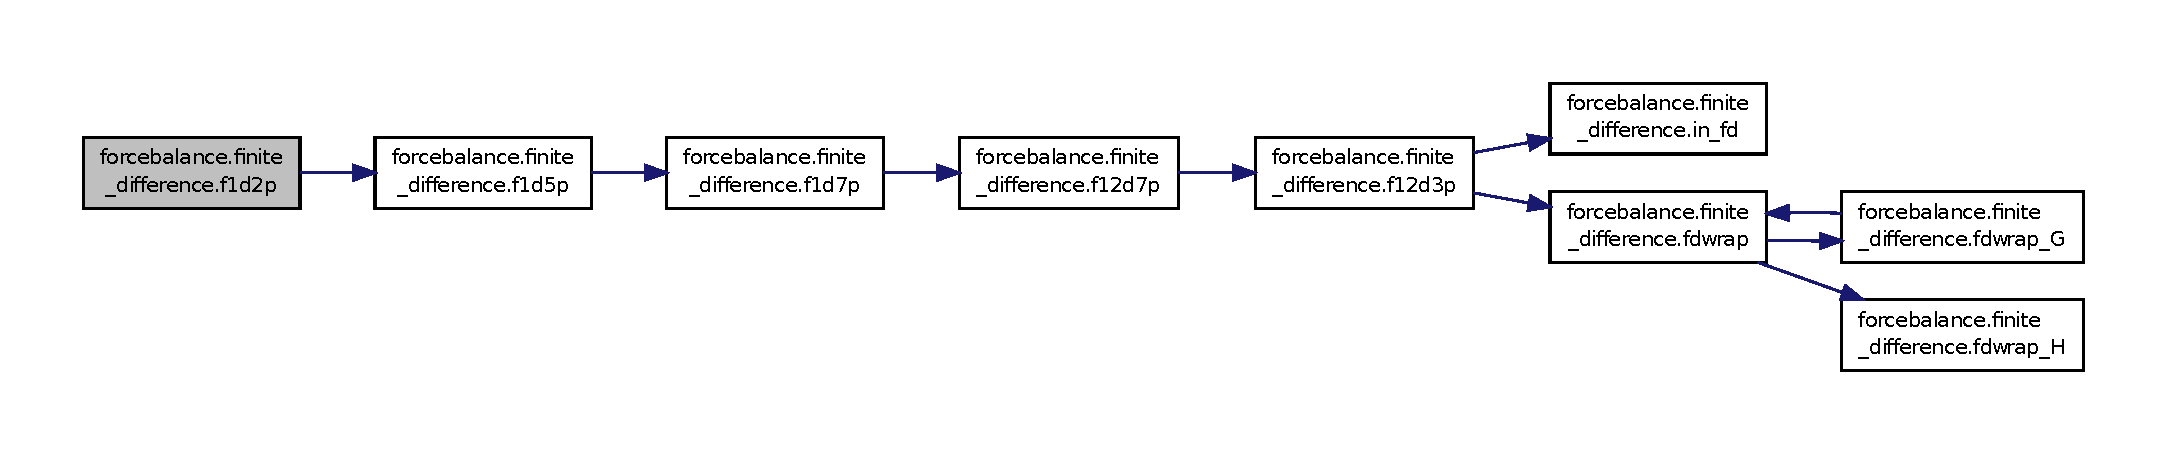
\includegraphics[width=350pt]{namespaceforcebalance_1_1finite__difference_ac5bb1552a9b8dd22c9c80e6444de2218_cgraph}
\end{center}
\end{figure}


\hypertarget{namespaceforcebalance_1_1finite__difference_a123c5d5dea0f3f50ab57796bb3bc39be}{\index{forcebalance\-::finite\-\_\-difference@{forcebalance\-::finite\-\_\-difference}!f1d5p@{f1d5p}}
\index{f1d5p@{f1d5p}!forcebalance::finite_difference@{forcebalance\-::finite\-\_\-difference}}
\paragraph[{f1d5p}]{\setlength{\rightskip}{0pt plus 5cm}def forcebalance.\-finite\-\_\-difference.\-f1d5p (
\begin{DoxyParamCaption}
\item[{}]{f, }
\item[{}]{h}
\end{DoxyParamCaption}
)}}\label{namespaceforcebalance_1_1finite__difference_a123c5d5dea0f3f50ab57796bb3bc39be}


A highly accurate five-\/point finite difference stencil for computing derivatives of a function. 

It works on both scalar and vector functions (i.\-e. functions that return arrays). Since the function does four computations, it's costly but recommended if we really need an accurate reference value.

The function is evaluated at points -\/2h, -\/h, +h and +2h and these values are combined to make the derivative according to\-: \href{http://www.holoborodko.com/pavel/numerical-methods/numerical-derivative/central-differences/}{\tt http\-://www.\-holoborodko.\-com/pavel/numerical-\/methods/numerical-\/derivative/central-\/differences/}

How to use\-: use fdwrap or something similar to generate a one-\/variable function from the (usually) much more complicated function that we wish to differentate. Then pass it to this function.

Inputs\-: f = The one-\/variable function f(x) that we're differentiating h = The finite difference step size, usually a small number

Outputs\-: fp = The finite difference derivative of the function f(x) around x=0. 

Definition at line 60 of file finite\-\_\-difference.\-py.



Here is the call graph for this function\-:\nopagebreak
\begin{figure}[H]
\begin{center}
\leavevmode
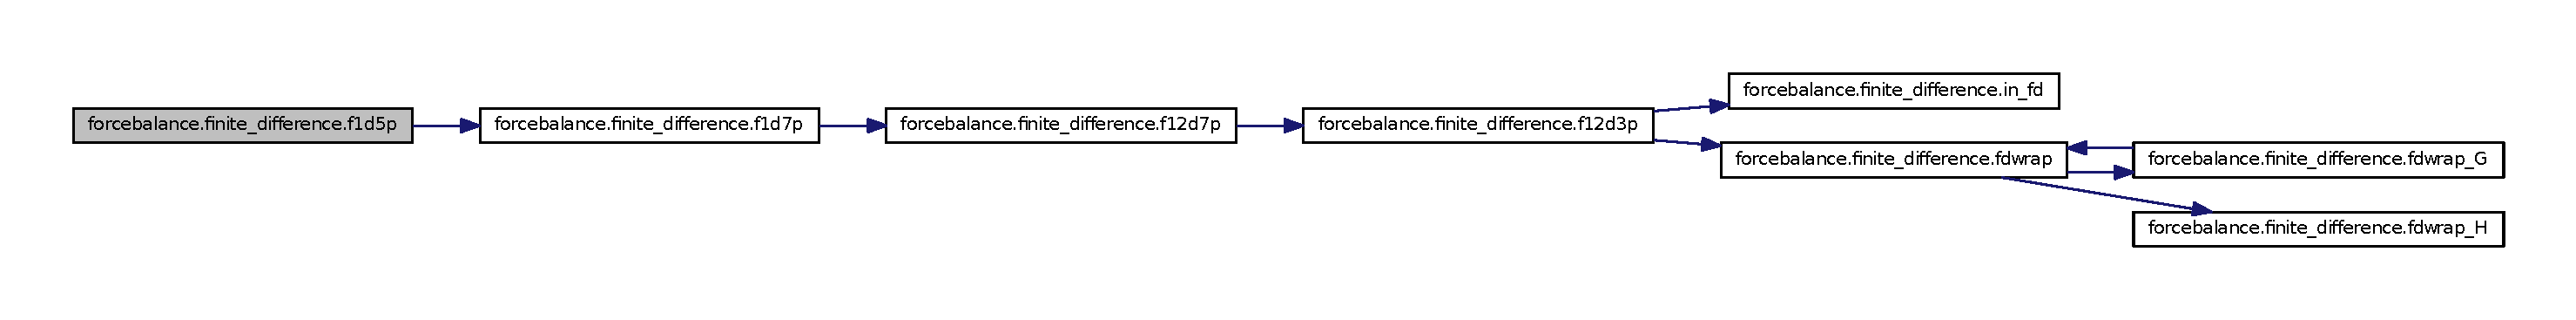
\includegraphics[width=350pt]{namespaceforcebalance_1_1finite__difference_a123c5d5dea0f3f50ab57796bb3bc39be_cgraph}
\end{center}
\end{figure}


\hypertarget{namespaceforcebalance_1_1finite__difference_a9be9f0d21300958092e380514e2e980d}{\index{forcebalance\-::finite\-\_\-difference@{forcebalance\-::finite\-\_\-difference}!f1d7p@{f1d7p}}
\index{f1d7p@{f1d7p}!forcebalance::finite_difference@{forcebalance\-::finite\-\_\-difference}}
\paragraph[{f1d7p}]{\setlength{\rightskip}{0pt plus 5cm}def forcebalance.\-finite\-\_\-difference.\-f1d7p (
\begin{DoxyParamCaption}
\item[{}]{f, }
\item[{}]{h}
\end{DoxyParamCaption}
)}}\label{namespaceforcebalance_1_1finite__difference_a9be9f0d21300958092e380514e2e980d}


A highly accurate seven-\/point finite difference stencil for computing derivatives of a function. 



Definition at line 70 of file finite\-\_\-difference.\-py.



Here is the call graph for this function\-:\nopagebreak
\begin{figure}[H]
\begin{center}
\leavevmode
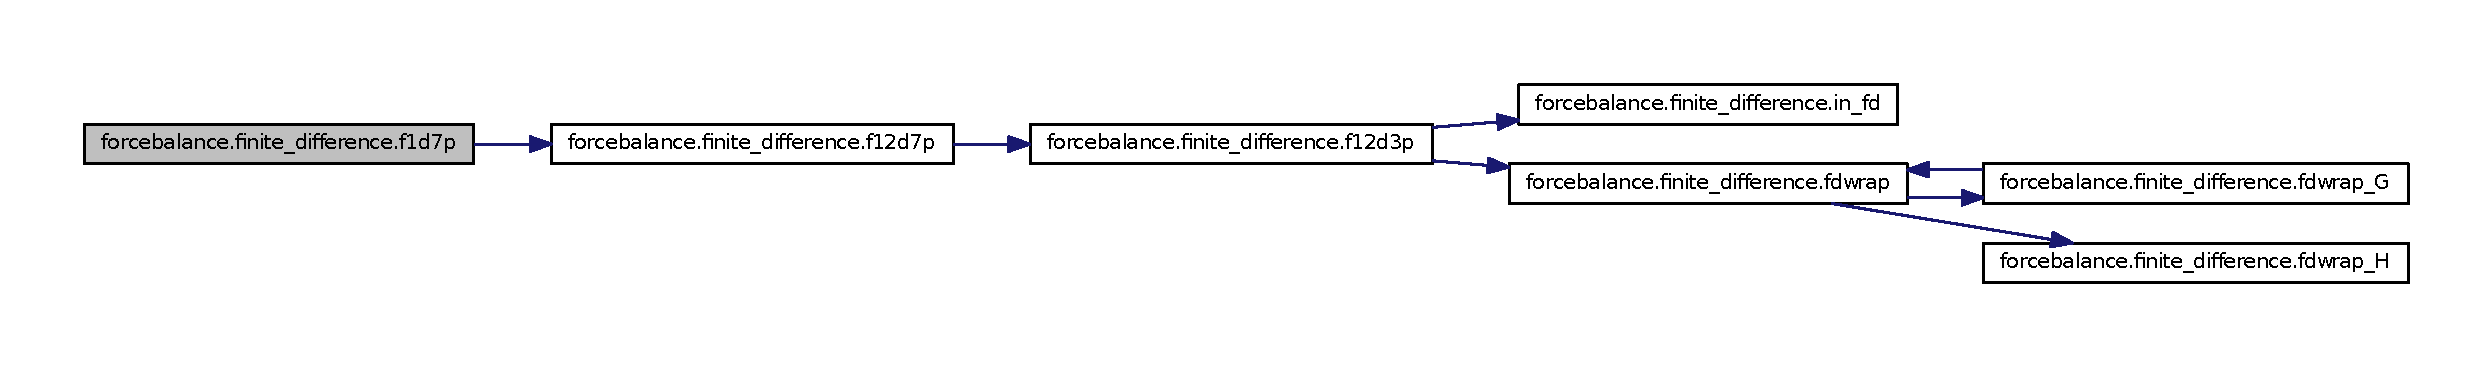
\includegraphics[width=350pt]{namespaceforcebalance_1_1finite__difference_a9be9f0d21300958092e380514e2e980d_cgraph}
\end{center}
\end{figure}


\hypertarget{namespaceforcebalance_1_1finite__difference_ae484c591ae8c4e5bae73a0ef2660c339}{\index{forcebalance\-::finite\-\_\-difference@{forcebalance\-::finite\-\_\-difference}!fdwrap@{fdwrap}}
\index{fdwrap@{fdwrap}!forcebalance::finite_difference@{forcebalance\-::finite\-\_\-difference}}
\paragraph[{fdwrap}]{\setlength{\rightskip}{0pt plus 5cm}def forcebalance.\-finite\-\_\-difference.\-fdwrap (
\begin{DoxyParamCaption}
\item[{}]{func, }
\item[{}]{mvals0, }
\item[{}]{pidx, }
\item[{}]{key = {\ttfamily None}, }
\item[{}]{kwargs}
\end{DoxyParamCaption}
)}}\label{namespaceforcebalance_1_1finite__difference_ae484c591ae8c4e5bae73a0ef2660c339}


A function wrapper for finite difference designed for differentiating 'get'-\/type functions. 

Since our finite difference stencils take single-\/variable functions and differentiate them around zero, and our objective function is quite a complicated function, we need a wrapper to serve as a middleman. The alternative would be to copy the finite difference formula to wherever we're taking the derivative, and that is prone to mistakes.

Inputs\-: func = Either get\-\_\-\-X or get\-\_\-\-G; these functions return dictionaries. \mbox{[}'X'\mbox{]} = 1.\-23, \mbox{[}'G'\mbox{]} = \mbox{[}0.\-12, 3,45, ...\mbox{]} mvals0 = The 'central' values of the mathematical parameters -\/ i.\-e. the wrapped function's origin is here. pidx = The index of the parameter that we're differentiating key = either 'G' or 'X', the value we wish to take out of the dictionary kwargs = Anything else we want to pass to the objective function (for instance, Project.\-Objective takes Order as an argument)

Outputs\-: func1 = Wrapped version of func, which takes a single float argument. 

Definition at line 147 of file finite\-\_\-difference.\-py.



Here is the call graph for this function\-:\nopagebreak
\begin{figure}[H]
\begin{center}
\leavevmode
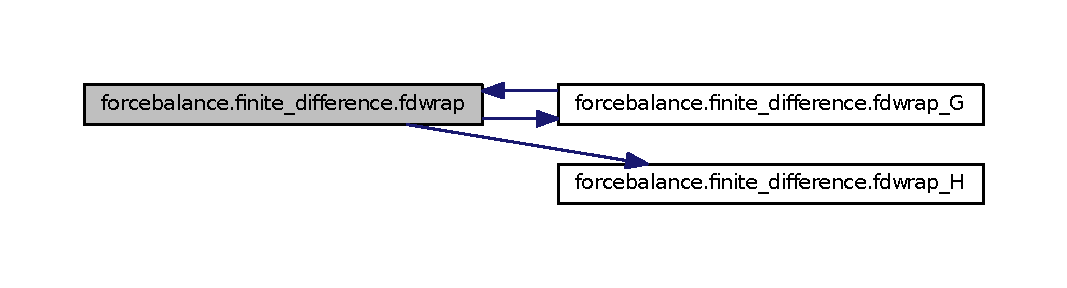
\includegraphics[width=336pt]{namespaceforcebalance_1_1finite__difference_ae484c591ae8c4e5bae73a0ef2660c339_cgraph}
\end{center}
\end{figure}


\hypertarget{namespaceforcebalance_1_1finite__difference_a00322fb65860c390616f74d05037c797}{\index{forcebalance\-::finite\-\_\-difference@{forcebalance\-::finite\-\_\-difference}!fdwrap\-\_\-\-G@{fdwrap\-\_\-\-G}}
\index{fdwrap\-\_\-\-G@{fdwrap\-\_\-\-G}!forcebalance::finite_difference@{forcebalance\-::finite\-\_\-difference}}
\paragraph[{fdwrap\-\_\-\-G}]{\setlength{\rightskip}{0pt plus 5cm}def forcebalance.\-finite\-\_\-difference.\-fdwrap\-\_\-\-G (
\begin{DoxyParamCaption}
\item[{}]{tgt, }
\item[{}]{mvals0, }
\item[{}]{pidx}
\end{DoxyParamCaption}
)}}\label{namespaceforcebalance_1_1finite__difference_a00322fb65860c390616f74d05037c797}


A driver to fdwrap for gradients (see documentation for fdwrap) Inputs\-: tgt = The Target containing the objective function that we want to differentiate mvals0 = The 'central' values of the mathematical parameters -\/ i.\-e. 

the wrapped function's origin is here. pidx = The index of the parameter that we're differentiating 

Definition at line 166 of file finite\-\_\-difference.\-py.



Here is the call graph for this function\-:\nopagebreak
\begin{figure}[H]
\begin{center}
\leavevmode
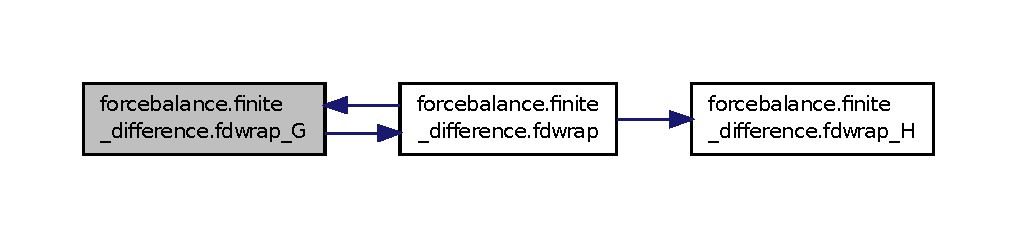
\includegraphics[width=350pt]{namespaceforcebalance_1_1finite__difference_a00322fb65860c390616f74d05037c797_cgraph}
\end{center}
\end{figure}


\hypertarget{namespaceforcebalance_1_1finite__difference_a77a0bc1ae3cbbcc8d38a0ef9ca877d6d}{\index{forcebalance\-::finite\-\_\-difference@{forcebalance\-::finite\-\_\-difference}!fdwrap\-\_\-\-H@{fdwrap\-\_\-\-H}}
\index{fdwrap\-\_\-\-H@{fdwrap\-\_\-\-H}!forcebalance::finite_difference@{forcebalance\-::finite\-\_\-difference}}
\paragraph[{fdwrap\-\_\-\-H}]{\setlength{\rightskip}{0pt plus 5cm}def forcebalance.\-finite\-\_\-difference.\-fdwrap\-\_\-\-H (
\begin{DoxyParamCaption}
\item[{}]{tgt, }
\item[{}]{mvals0, }
\item[{}]{pidx}
\end{DoxyParamCaption}
)}}\label{namespaceforcebalance_1_1finite__difference_a77a0bc1ae3cbbcc8d38a0ef9ca877d6d}


A driver to fdwrap for Hessians (see documentation for fdwrap) Inputs\-: tgt = The Target containing the objective function that we want to differentiate mvals0 = The 'central' values of the mathematical parameters -\/ i.\-e. 

the wrapped function's origin is here. pidx = The index of the parameter that we're differentiating 

Definition at line 177 of file finite\-\_\-difference.\-py.

\hypertarget{namespaceforcebalance_1_1finite__difference_ad84d3e385db1190e7d8ef58bc08a6c52}{\index{forcebalance\-::finite\-\_\-difference@{forcebalance\-::finite\-\_\-difference}!in\-\_\-fd@{in\-\_\-fd}}
\index{in\-\_\-fd@{in\-\_\-fd}!forcebalance::finite_difference@{forcebalance\-::finite\-\_\-difference}}
\paragraph[{in\-\_\-fd}]{\setlength{\rightskip}{0pt plus 5cm}def forcebalance.\-finite\-\_\-difference.\-in\-\_\-fd (
\begin{DoxyParamCaption}
{}
\end{DoxyParamCaption}
)}}\label{namespaceforcebalance_1_1finite__difference_ad84d3e385db1190e7d8ef58bc08a6c52}


Invoking this function from anywhere will tell us whether we're being called by a finite-\/difference function. 

This is mainly useful for deciding when to update the 'qualitative indicators' and when not to. 

Definition at line 121 of file finite\-\_\-difference.\-py.



\subsubsection{Variable Documentation}
\hypertarget{namespaceforcebalance_1_1finite__difference_a2bdf74505c45f442e1c96d557414254e}{\index{forcebalance\-::finite\-\_\-difference@{forcebalance\-::finite\-\_\-difference}!logger@{logger}}
\index{logger@{logger}!forcebalance::finite_difference@{forcebalance\-::finite\-\_\-difference}}
\paragraph[{logger}]{\setlength{\rightskip}{0pt plus 5cm}tuple forcebalance.\-finite\-\_\-difference.\-logger = get\-Logger(\-\_\-\-\_\-name\-\_\-\-\_\-)}}\label{namespaceforcebalance_1_1finite__difference_a2bdf74505c45f442e1c96d557414254e}


Definition at line 7 of file finite\-\_\-difference.\-py.


\hypertarget{namespaceforcebalance_1_1forcefield}{\subsection{forcebalance.\-forcefield Namespace Reference}
\label{namespaceforcebalance_1_1forcefield}\index{forcebalance.\-forcefield@{forcebalance.\-forcefield}}
}


Force field module.  


\subsubsection*{Classes}
\begin{DoxyCompactItemize}
\item 
class \hyperlink{classforcebalance_1_1forcefield_1_1BackedUpDict}{Backed\-Up\-Dict}
\item 
class \hyperlink{classforcebalance_1_1forcefield_1_1FF}{F\-F}
\begin{DoxyCompactList}\small\item\em Force field class. \end{DoxyCompactList}\end{DoxyCompactItemize}
\subsubsection*{Functions}
\begin{DoxyCompactItemize}
\item 
def \hyperlink{namespaceforcebalance_1_1forcefield_a99c9997d5158a04be089f291bd6f99bd}{determine\-\_\-fftype}
\begin{DoxyCompactList}\small\item\em Determine the type of a force field file. \end{DoxyCompactList}\item 
def \hyperlink{namespaceforcebalance_1_1forcefield_ab1a855bace20dd5e45928467e2a133f1}{rs\-\_\-override}
\begin{DoxyCompactList}\small\item\em This function takes in a dictionary (rsfactors) and a string (termtype). \end{DoxyCompactList}\end{DoxyCompactItemize}
\subsubsection*{Variables}
\begin{DoxyCompactItemize}
\item 
dictionary \hyperlink{namespaceforcebalance_1_1forcefield_abc5e12aa78c5742f028b954ede086c51}{F\-F\-\_\-\-Extensions}
\item 
dictionary \hyperlink{namespaceforcebalance_1_1forcefield_a3beac9806e0438b79b9ae60a47c7b131}{F\-F\-\_\-\-I\-O\-Modules}
\end{DoxyCompactItemize}


\subsubsection{Detailed Description}
Force field module. In Force\-Balance a 'force field' is built from a set of files containing physical parameters. These files can be anything that enter into any computation -\/ our original program was quite dependent on the G\-R\-O\-M\-A\-C\-S force field format, but this program is set up to allow very general input formats.

We introduce several important concepts\-:

1) Adjustable parameters are allocated into a vector.

To cast the force field optimization as a math problem, we treat all of the parameters on equal footing and write them as indices in a parameter vector.

2) A mapping from interaction type to parameter number.

Each element in the parameter vector corresponds to one or more interaction types. Whenever we change the parameter vector and recompute the objective function, this amounts to changing the physical parameters in the simulations, so we print out new force field files for external programs. In addition, when these programs are computing the objective function we are often in low-\/level subroutines that compute terms in the energy and force. If we need an analytic derivative of the objective function, then these subroutines need to know which index of the parameter vector needs to be modified.

This is done by way of a hash table\-: for example, when we are computing a Coulomb interaction between atom 4 and atom 5, we can build the words 'C\-O\-U\-L4' and 'C\-O\-U\-L5' and look it up in the parameter map; this gives us two numbers (say, 10 and 11) corresponding to the eleventh and twelfth element of the parameter vector. Then we can compute the derivatives of the energy w/r.\-t. these parameters (in this case, C\-O\-U\-L5/rij and C\-O\-U\-L4/rij) and increment these values in the objective function gradient.

In custom-\/implemented force fields (see counterpoisematch.\-py) the hash table can also be used to look up parameter values for computation of interactions. This is probably not the fastest way to do things, however.

3) Distinction between physical and mathematical parameters.

The optimization algorithm works in a space that is related to, but not exactly the same as the physical parameter space. The reasons for why we do this are\-:

a) Each parameter has its own physical units. On the one hand it's not right to treat different physical units all on the same footing, so nondimensionalization is desirable. To make matters worse, the force field parameters can be small as 1e-\/8 or as large as 1e+6 depending on the parameter type. This means the elements of the objective function gradient / Hessian have elements that differ from each other in size by 10+ orders of magnitude, leading to mathematical instabilities in the optimizer.

b) The parameter space can be constrained, most notably for atomic partial charges where we don't want to change the overall charge on a molecule. Thus we wish to project out certain movements in the mathematical parameters such that they don't change the physical parameters.

c) We wish to regularize our optimization so as to avoid changing our parameters in very insensitive directions (linear dependencies). However, the sensitivity of the objective function to changes in the force field depends on the physical units!

For all of these reasons, we introduce a 'transformation matrix' which maps mathematical parameters onto physical parameters. The diagonal elements in this matrix are rescaling factors; they take the mathematical parameter and magnify it by this constant factor. The off-\/diagonal elements correspond to rotations and other linear transformations, and currently I just use them to project out the 'increase the net charge' direction in the physical parameter space.

Note that with regularization, these rescaling factors are equivalent to the widths of prior distributions in a maximum likelihood framework. Because there is such a correspondence between rescaling factors and choosing a prior, they need to be chosen carefully. This is work in progress. Another possibility is to sample the width of the priors from a noninformative distribution -- the hyperprior (we can choose the Jeffreys prior or something). This is work in progress.

Right now only G\-R\-O\-M\-A\-C\-S parameters are supported, but this class is extensible, we need more modules!

\begin{DoxyAuthor}{Author}
Lee-\/\-Ping Wang 
\end{DoxyAuthor}
\begin{DoxyDate}{Date}
04/2012 
\end{DoxyDate}


\subsubsection{Function Documentation}
\hypertarget{namespaceforcebalance_1_1forcefield_a99c9997d5158a04be089f291bd6f99bd}{\index{forcebalance\-::forcefield@{forcebalance\-::forcefield}!determine\-\_\-fftype@{determine\-\_\-fftype}}
\index{determine\-\_\-fftype@{determine\-\_\-fftype}!forcebalance::forcefield@{forcebalance\-::forcefield}}
\paragraph[{determine\-\_\-fftype}]{\setlength{\rightskip}{0pt plus 5cm}def forcebalance.\-forcefield.\-determine\-\_\-fftype (
\begin{DoxyParamCaption}
\item[{}]{ffname, }
\item[{}]{verbose = {\ttfamily False}}
\end{DoxyParamCaption}
)}}\label{namespaceforcebalance_1_1forcefield_a99c9997d5158a04be089f291bd6f99bd}


Determine the type of a force field file. 

It is possible to specify the file type explicitly in the input file using the syntax 'force\-\_\-field.\-ext\-:type'. Otherwise this function will try to determine the force field type by extension. 

Definition at line 143 of file forcefield.\-py.

\hypertarget{namespaceforcebalance_1_1forcefield_ab1a855bace20dd5e45928467e2a133f1}{\index{forcebalance\-::forcefield@{forcebalance\-::forcefield}!rs\-\_\-override@{rs\-\_\-override}}
\index{rs\-\_\-override@{rs\-\_\-override}!forcebalance::forcefield@{forcebalance\-::forcefield}}
\paragraph[{rs\-\_\-override}]{\setlength{\rightskip}{0pt plus 5cm}def forcebalance.\-forcefield.\-rs\-\_\-override (
\begin{DoxyParamCaption}
\item[{}]{rsfactors, }
\item[{}]{termtype, }
\item[{}]{Temperature = {\ttfamily 298.15}}
\end{DoxyParamCaption}
)}}\label{namespaceforcebalance_1_1forcefield_ab1a855bace20dd5e45928467e2a133f1}


This function takes in a dictionary (rsfactors) and a string (termtype). 

\begin{DoxyVerb} If termtype matches any of the strings below, rsfactors[termtype] is assigned
 to one of the numbers below.

 This is LPW's attempt to simplify the rescaling factors.
\end{DoxyVerb}



\begin{DoxyParams}[1]{Parameters}
\mbox{\tt out}  & {\em rsfactors} & The computed rescaling factor. \\
\hline
\mbox{\tt in}  & {\em termtype} & The interaction type (corresponding to a physical unit) \\
\hline
\mbox{\tt in}  & {\em Temperature} & The temperature for computing the k\-T energy scale \\
\hline
\end{DoxyParams}


Definition at line 1171 of file forcefield.\-py.



\subsubsection{Variable Documentation}
\hypertarget{namespaceforcebalance_1_1forcefield_abc5e12aa78c5742f028b954ede086c51}{\index{forcebalance\-::forcefield@{forcebalance\-::forcefield}!F\-F\-\_\-\-Extensions@{F\-F\-\_\-\-Extensions}}
\index{F\-F\-\_\-\-Extensions@{F\-F\-\_\-\-Extensions}!forcebalance::forcefield@{forcebalance\-::forcefield}}
\paragraph[{F\-F\-\_\-\-Extensions}]{\setlength{\rightskip}{0pt plus 5cm}dictionary forcebalance.\-forcefield.\-F\-F\-\_\-\-Extensions}}\label{namespaceforcebalance_1_1forcefield_abc5e12aa78c5742f028b954ede086c51}
{\bfseries Initial value\-:}
\begin{DoxyCode}
1 = \{\textcolor{stringliteral}{"itp"} : \textcolor{stringliteral}{"gmx"},
2                  \textcolor{stringliteral}{"in"}  : \textcolor{stringliteral}{"qchem"},
3                  \textcolor{stringliteral}{"prm"} : \textcolor{stringliteral}{"tinker"},
4                  \textcolor{stringliteral}{"gen"} : \textcolor{stringliteral}{"custom"},
5                  \textcolor{stringliteral}{"xml"} : \textcolor{stringliteral}{"openmm"},
6                  \textcolor{stringliteral}{"frcmod"} : \textcolor{stringliteral}{"frcmod"},
7                  \textcolor{stringliteral}{"mol2"} : \textcolor{stringliteral}{"mol2"},
8                  \textcolor{stringliteral}{"gbs"}  : \textcolor{stringliteral}{"gbs"},
9                  \textcolor{stringliteral}{"grid"} : \textcolor{stringliteral}{"grid"}
10                  \}
\end{DoxyCode}


Definition at line 115 of file forcefield.\-py.

\hypertarget{namespaceforcebalance_1_1forcefield_a3beac9806e0438b79b9ae60a47c7b131}{\index{forcebalance\-::forcefield@{forcebalance\-::forcefield}!F\-F\-\_\-\-I\-O\-Modules@{F\-F\-\_\-\-I\-O\-Modules}}
\index{F\-F\-\_\-\-I\-O\-Modules@{F\-F\-\_\-\-I\-O\-Modules}!forcebalance::forcefield@{forcebalance\-::forcefield}}
\paragraph[{F\-F\-\_\-\-I\-O\-Modules}]{\setlength{\rightskip}{0pt plus 5cm}dictionary forcebalance.\-forcefield.\-F\-F\-\_\-\-I\-O\-Modules}}\label{namespaceforcebalance_1_1forcefield_a3beac9806e0438b79b9ae60a47c7b131}
{\bfseries Initial value\-:}
\begin{DoxyCode}
1 = \{\textcolor{stringliteral}{"gmx"}: \hyperlink{classforcebalance_1_1gmxio_1_1ITP__Reader}{gmxio.ITP\_Reader} ,
2                 \textcolor{stringliteral}{"qchem"}: \hyperlink{classforcebalance_1_1qchemio_1_1QCIn__Reader}{qchemio.QCIn\_Reader} ,
3                 \textcolor{stringliteral}{"tinker"}: \hyperlink{classforcebalance_1_1tinkerio_1_1Tinker__Reader}{tinkerio.Tinker\_Reader} ,
4                 \textcolor{stringliteral}{"custom"}: \hyperlink{classforcebalance_1_1custom__io_1_1Gen__Reader}{custom\_io.Gen\_Reader} , 
5                 \textcolor{stringliteral}{"openmm"} : \hyperlink{classforcebalance_1_1openmmio_1_1OpenMM__Reader}{openmmio.OpenMM\_Reader},
6                 \textcolor{stringliteral}{"frcmod"} : \hyperlink{classforcebalance_1_1amberio_1_1FrcMod__Reader}{amberio.FrcMod\_Reader},
7                 \textcolor{stringliteral}{"mol2"} : \hyperlink{classforcebalance_1_1amberio_1_1Mol2__Reader}{amberio.Mol2\_Reader},
8                 \textcolor{stringliteral}{"gbs"} : \hyperlink{classforcebalance_1_1psi4io_1_1GBS__Reader}{psi4io.GBS\_Reader},
9                 \textcolor{stringliteral}{"grid"} : \hyperlink{classforcebalance_1_1psi4io_1_1Grid__Reader}{psi4io.Grid\_Reader}
10                 \}
\end{DoxyCode}


Definition at line 127 of file forcefield.\-py.


\hypertarget{namespaceforcebalance_1_1gmxio}{\subsection{forcebalance\-:\-:gmxio \-Namespace \-Reference}
\label{namespaceforcebalance_1_1gmxio}\index{forcebalance\-::gmxio@{forcebalance\-::gmxio}}
}


\-G\-R\-O\-M\-A\-C\-S input/output.  


\subsubsection*{\-Classes}
\begin{DoxyCompactItemize}
\item 
class \hyperlink{classforcebalance_1_1gmxio_1_1ITP__Reader}{\-I\-T\-P\-\_\-\-Reader}
\begin{DoxyCompactList}\small\item\em \-Finite state machine for parsing \-G\-R\-O\-M\-A\-C\-S force field files. \end{DoxyCompactList}\item 
class \hyperlink{classforcebalance_1_1gmxio_1_1AbInitio__GMX}{\-Ab\-Initio\-\_\-\-G\-M\-X}
\begin{DoxyCompactList}\small\item\em \-Subclass of \-Ab\-Initio for force and energy matching using normal \-G\-R\-O\-M\-A\-C\-S. \end{DoxyCompactList}\item 
class \hyperlink{classforcebalance_1_1gmxio_1_1Liquid__GMX}{\-Liquid\-\_\-\-G\-M\-X}
\item 
class \hyperlink{classforcebalance_1_1gmxio_1_1Interaction__GMX}{\-Interaction\-\_\-\-G\-M\-X}
\begin{DoxyCompactList}\small\item\em \-Subclass of \-Interaction for interaction energy matching using \-G\-R\-O\-M\-A\-C\-S. \end{DoxyCompactList}\end{DoxyCompactItemize}
\subsubsection*{\-Functions}
\begin{DoxyCompactItemize}
\item 
def \hyperlink{namespaceforcebalance_1_1gmxio_acc5bef2c5c991cd70a948a1dd43ef6a6}{edit\-\_\-mdp}
\begin{DoxyCompactList}\small\item\em \-Create or edit a \-Gromacs \-M\-D\-P file. \end{DoxyCompactList}\item 
def \hyperlink{namespaceforcebalance_1_1gmxio_a29af6ace00d7e58258e0a854ca13d954}{parse\-\_\-atomtype\-\_\-line}
\begin{DoxyCompactList}\small\item\em \-Parses the 'atomtype' line. \end{DoxyCompactList}\item 
def \hyperlink{namespaceforcebalance_1_1gmxio_acac8488f29b62fb0d4cb54bb5a041026}{rm\-\_\-gmx\-\_\-baks}
\end{DoxyCompactItemize}
\subsubsection*{\-Variables}
\begin{DoxyCompactItemize}
\item 
tuple \hyperlink{namespaceforcebalance_1_1gmxio_a1ba0eaad8ffef47e3afff245dd1e3dcf}{logger} = get\-Logger(\-\_\-\-\_\-name\-\_\-\-\_\-)
\item 
list \hyperlink{namespaceforcebalance_1_1gmxio_a1273a5830d780475a2d07385c60341f6}{nftypes} = \mbox{[}\-None, '\-V\-D\-W', '\-V\-D\-W\-\_\-\-B\-H\-A\-M'\mbox{]}
\begin{DoxyCompactList}\small\item\em \-Vd\-W interaction function types. \end{DoxyCompactList}\item 
list \hyperlink{namespaceforcebalance_1_1gmxio_a1e3fab50f3ebc3477ff3fb31671e840b}{pftypes} = \mbox{[}\-None, '\-V\-P\-A\-I\-R', '\-V\-P\-A\-I\-R\-\_\-\-B\-H\-A\-M'\mbox{]}
\begin{DoxyCompactList}\small\item\em \-Pairwise interaction function types. \end{DoxyCompactList}\item 
list \hyperlink{namespaceforcebalance_1_1gmxio_ac8e059e7c8d46326654f585b23f2d0b0}{bftypes} = \mbox{[}\-None, '\-B\-O\-N\-D\-S', '\-G96\-B\-O\-N\-D\-S', '\-M\-O\-R\-S\-E'\mbox{]}
\begin{DoxyCompactList}\small\item\em \-Bonded interaction function types. \end{DoxyCompactList}\item 
list \hyperlink{namespaceforcebalance_1_1gmxio_ac655fded3f739845c1a803fc4123a593}{aftypes}
\begin{DoxyCompactList}\small\item\em \-Angle interaction function types. \end{DoxyCompactList}\item 
list \hyperlink{namespaceforcebalance_1_1gmxio_a5520b315e210120bb3e14af3665d568c}{dftypes} = \mbox{[}\-None, '\-P\-D\-I\-H\-S', '\-I\-D\-I\-H\-S', '\-R\-B\-D\-I\-H\-S', '\-P\-I\-M\-P\-D\-I\-H\-S', '\-F\-O\-U\-R\-D\-I\-H\-S', \-None, \-None, '\-T\-A\-B\-D\-I\-H\-S', '\-P\-D\-I\-H\-M\-U\-L\-S'\mbox{]}
\begin{DoxyCompactList}\small\item\em \-Dihedral interaction function types. \end{DoxyCompactList}\item 
dictionary \hyperlink{namespaceforcebalance_1_1gmxio_ac4e46dd6adabe0dfdeddcd86e772ad33}{fdict}
\begin{DoxyCompactList}\small\item\em \-Section -\/$>$ \-Interaction type dictionary. \end{DoxyCompactList}\item 
dictionary \hyperlink{namespaceforcebalance_1_1gmxio_afa3ee5e262ff005d87d20b4ec1581bad}{pdict}
\begin{DoxyCompactList}\small\item\em \-Interaction type -\/$>$ \-Parameter \-Dictionary. \end{DoxyCompactList}\end{DoxyCompactItemize}


\subsubsection{\-Detailed \-Description}
\-G\-R\-O\-M\-A\-C\-S input/output. \begin{DoxyRefDesc}{\-Todo}
\item[\hyperlink{todo__todo000009}{\-Todo}]\-Even more stuff from \hyperlink{forcefield_8py}{forcefield.\-py} needs to go into here.\end{DoxyRefDesc}


\begin{DoxyAuthor}{\-Author}
\-Lee-\/\-Ping \-Wang 
\end{DoxyAuthor}
\begin{DoxyDate}{\-Date}
12/2011
\end{DoxyDate}
\begin{DoxyRefDesc}{\-Todo}
\item[\hyperlink{todo__todo000012}{\-Todo}]\-Even more stuff from \hyperlink{forcefield_8py}{forcefield.\-py} needs to go into here.\end{DoxyRefDesc}


\begin{DoxyAuthor}{\-Author}
\-Lee-\/\-Ping \-Wang 
\end{DoxyAuthor}
\begin{DoxyDate}{\-Date}
12/2011 
\end{DoxyDate}


\subsubsection{\-Function \-Documentation}
\hypertarget{namespaceforcebalance_1_1gmxio_acc5bef2c5c991cd70a948a1dd43ef6a6}{\index{forcebalance\-::gmxio@{forcebalance\-::gmxio}!edit\-\_\-mdp@{edit\-\_\-mdp}}
\index{edit\-\_\-mdp@{edit\-\_\-mdp}!forcebalance::gmxio@{forcebalance\-::gmxio}}
\paragraph[{edit\-\_\-mdp}]{\setlength{\rightskip}{0pt plus 5cm}def {\bf forcebalance.\-gmxio.\-edit\-\_\-mdp} (
\begin{DoxyParamCaption}
\item[{}]{fin, }
\item[{}]{fout, }
\item[{}]{options, }
\item[{}]{verbose = {\ttfamily \-False}}
\end{DoxyParamCaption}
)}}\label{namespaceforcebalance_1_1gmxio_acc5bef2c5c991cd70a948a1dd43ef6a6}


\-Create or edit a \-Gromacs \-M\-D\-P file. 


\begin{DoxyParams}[1]{\-Parameters}
\mbox{\tt in}  & {\em fin} & \-Input file name. \\
\hline
\mbox{\tt in}  & {\em fout} & \-Output file name, can be the same as input file name. \\
\hline
\mbox{\tt in}  & {\em options} & \-Dictionary containing mdp options. \-Existing options are replaced, new options are added at the end. \\
\hline
\end{DoxyParams}


\-Definition at line 35 of file gmxio.\-py.



\-Here is the call graph for this function\-:
\nopagebreak
\begin{figure}[H]
\begin{center}
\leavevmode
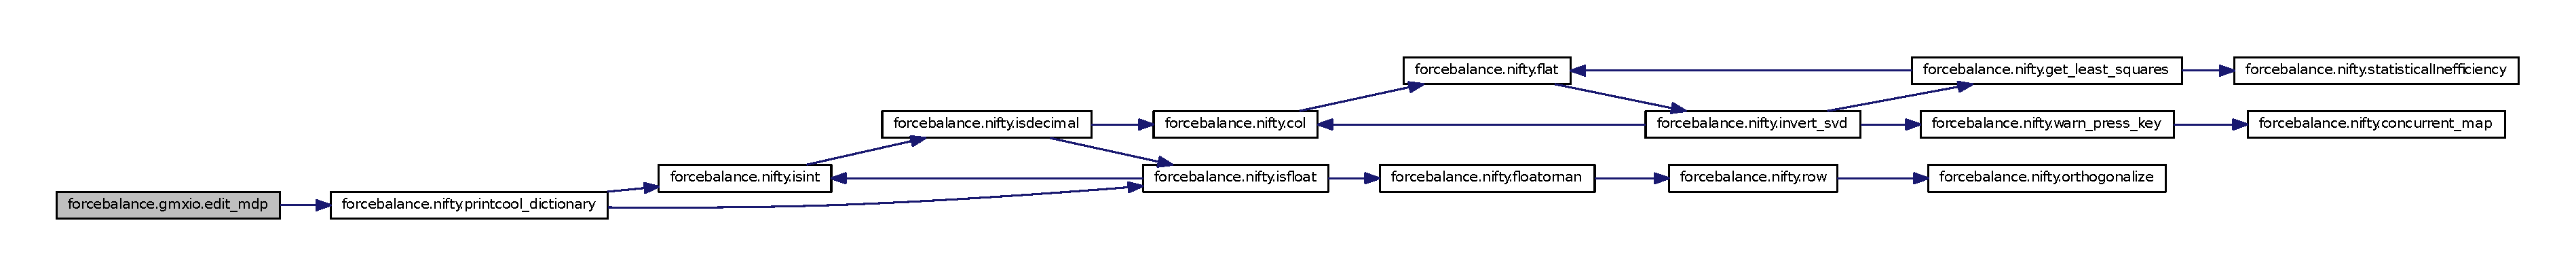
\includegraphics[width=350pt]{namespaceforcebalance_1_1gmxio_acc5bef2c5c991cd70a948a1dd43ef6a6_cgraph}
\end{center}
\end{figure}


\hypertarget{namespaceforcebalance_1_1gmxio_a29af6ace00d7e58258e0a854ca13d954}{\index{forcebalance\-::gmxio@{forcebalance\-::gmxio}!parse\-\_\-atomtype\-\_\-line@{parse\-\_\-atomtype\-\_\-line}}
\index{parse\-\_\-atomtype\-\_\-line@{parse\-\_\-atomtype\-\_\-line}!forcebalance::gmxio@{forcebalance\-::gmxio}}
\paragraph[{parse\-\_\-atomtype\-\_\-line}]{\setlength{\rightskip}{0pt plus 5cm}def {\bf forcebalance.\-gmxio.\-parse\-\_\-atomtype\-\_\-line} (
\begin{DoxyParamCaption}
\item[{}]{line}
\end{DoxyParamCaption}
)}}\label{namespaceforcebalance_1_1gmxio_a29af6ace00d7e58258e0a854ca13d954}


\-Parses the 'atomtype' line. 

\-Parses lines like this\-:\par
 {\ttfamily  opls\-\_\-135 \-C\-T 6 12.\-0107 0.\-0000 \-A 3.\-5000e-\/01 2.\-7614e-\/01\par
 \-C 12.\-0107 0.\-0000 \-A 3.\-7500e-\/01 4.\-3932e-\/01\par
 \-Na 11 22.\-9897 0.\-0000 \-A 6.\-068128070229e+03 2.\-662662556402e+01 0.\-0000e+00 ; \-P\-A\-R\-M 5 6\par
 } \-Look at all the variety!


\begin{DoxyParams}[1]{\-Parameters}
\mbox{\tt in}  & {\em line} & \-Input line. \\
\hline
\end{DoxyParams}
\begin{DoxyReturn}{\-Returns}
answer \-Dictionary containing\-:\par
 atom type\par
 bonded atom type (if any)\par
 atomic number (if any)\par
 atomic mass\par
 charge\par
 particle type\par
 force field parameters\par
 number of optional fields 
\end{DoxyReturn}


\-Definition at line 181 of file gmxio.\-py.



\-Here is the call graph for this function\-:
\nopagebreak
\begin{figure}[H]
\begin{center}
\leavevmode
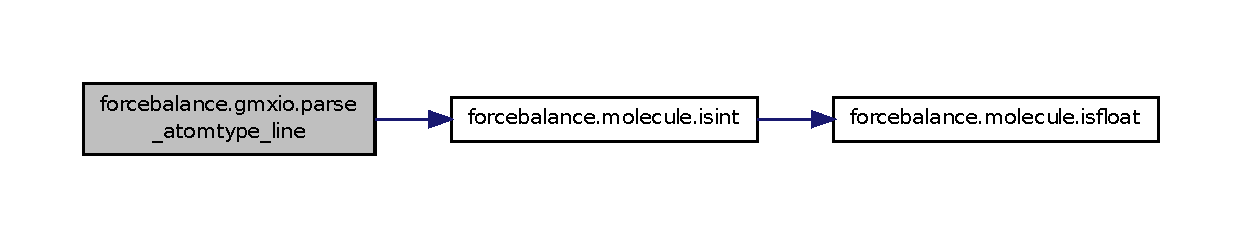
\includegraphics[width=350pt]{namespaceforcebalance_1_1gmxio_a29af6ace00d7e58258e0a854ca13d954_cgraph}
\end{center}
\end{figure}


\hypertarget{namespaceforcebalance_1_1gmxio_acac8488f29b62fb0d4cb54bb5a041026}{\index{forcebalance\-::gmxio@{forcebalance\-::gmxio}!rm\-\_\-gmx\-\_\-baks@{rm\-\_\-gmx\-\_\-baks}}
\index{rm\-\_\-gmx\-\_\-baks@{rm\-\_\-gmx\-\_\-baks}!forcebalance::gmxio@{forcebalance\-::gmxio}}
\paragraph[{rm\-\_\-gmx\-\_\-baks}]{\setlength{\rightskip}{0pt plus 5cm}def {\bf forcebalance.\-gmxio.\-rm\-\_\-gmx\-\_\-baks} (
\begin{DoxyParamCaption}
\item[{}]{dir}
\end{DoxyParamCaption}
)}}\label{namespaceforcebalance_1_1gmxio_acac8488f29b62fb0d4cb54bb5a041026}


\-Definition at line 428 of file gmxio.\-py.



\subsubsection{\-Variable \-Documentation}
\hypertarget{namespaceforcebalance_1_1gmxio_ac655fded3f739845c1a803fc4123a593}{\index{forcebalance\-::gmxio@{forcebalance\-::gmxio}!aftypes@{aftypes}}
\index{aftypes@{aftypes}!forcebalance::gmxio@{forcebalance\-::gmxio}}
\paragraph[{aftypes}]{\setlength{\rightskip}{0pt plus 5cm}list {\bf forcebalance\-::gmxio\-::aftypes}}}\label{namespaceforcebalance_1_1gmxio_ac655fded3f739845c1a803fc4123a593}
{\bfseries \-Initial value\-:}
\begin{DoxyCode}
1 [None, 'ANGLES', 'G96ANGLES', 'CROSS_BOND_BOND',
2            'CROSS_BOND_ANGLE', 'UREY_BRADLEY', 'QANGLES']
\end{DoxyCode}


\-Angle interaction function types. 



\-Definition at line 91 of file gmxio.\-py.

\hypertarget{namespaceforcebalance_1_1gmxio_ac8e059e7c8d46326654f585b23f2d0b0}{\index{forcebalance\-::gmxio@{forcebalance\-::gmxio}!bftypes@{bftypes}}
\index{bftypes@{bftypes}!forcebalance::gmxio@{forcebalance\-::gmxio}}
\paragraph[{bftypes}]{\setlength{\rightskip}{0pt plus 5cm}list {\bf forcebalance\-::gmxio\-::bftypes} = \mbox{[}\-None, '\-B\-O\-N\-D\-S', '\-G96\-B\-O\-N\-D\-S', '\-M\-O\-R\-S\-E'\mbox{]}}}\label{namespaceforcebalance_1_1gmxio_ac8e059e7c8d46326654f585b23f2d0b0}


\-Bonded interaction function types. 



\-Definition at line 89 of file gmxio.\-py.

\hypertarget{namespaceforcebalance_1_1gmxio_a5520b315e210120bb3e14af3665d568c}{\index{forcebalance\-::gmxio@{forcebalance\-::gmxio}!dftypes@{dftypes}}
\index{dftypes@{dftypes}!forcebalance::gmxio@{forcebalance\-::gmxio}}
\paragraph[{dftypes}]{\setlength{\rightskip}{0pt plus 5cm}list {\bf forcebalance\-::gmxio\-::dftypes} = \mbox{[}\-None, '\-P\-D\-I\-H\-S', '\-I\-D\-I\-H\-S', '\-R\-B\-D\-I\-H\-S', '\-P\-I\-M\-P\-D\-I\-H\-S', '\-F\-O\-U\-R\-D\-I\-H\-S', \-None, \-None, '\-T\-A\-B\-D\-I\-H\-S', '\-P\-D\-I\-H\-M\-U\-L\-S'\mbox{]}}}\label{namespaceforcebalance_1_1gmxio_a5520b315e210120bb3e14af3665d568c}


\-Dihedral interaction function types. 



\-Definition at line 94 of file gmxio.\-py.

\hypertarget{namespaceforcebalance_1_1gmxio_ac4e46dd6adabe0dfdeddcd86e772ad33}{\index{forcebalance\-::gmxio@{forcebalance\-::gmxio}!fdict@{fdict}}
\index{fdict@{fdict}!forcebalance::gmxio@{forcebalance\-::gmxio}}
\paragraph[{fdict}]{\setlength{\rightskip}{0pt plus 5cm}dictionary {\bf forcebalance\-::gmxio\-::fdict}}}\label{namespaceforcebalance_1_1gmxio_ac4e46dd6adabe0dfdeddcd86e772ad33}
{\bfseries \-Initial value\-:}
\begin{DoxyCode}
1 {
2     'atomtypes'     : nftypes,
3     'nonbond_params': pftypes,
4     'bonds'         : bftypes,
5     'bondtypes'     : bftypes,
6     'angles'        : aftypes,
7     'angletypes'    : aftypes,
8     'dihedrals'     : dftypes,
9     'dihedraltypes' : dftypes,
10     'virtual_sites2': ['NONE','VSITE2'],
11     'virtual_sites3': ['NONE','VSITE3','VSITE3FD','VSITE3FAD','VSITE3OUT'],
12     'virtual_sites4': ['NONE','VSITE4FD','VSITE4FDN']
13     }
\end{DoxyCode}


\-Section -\/$>$ \-Interaction type dictionary. 

\-Based on the section you're in and the integer given on the current line, this looks up the 'interaction type' -\/ for example, within bonded interactions there are four interaction types\-: harmonic, \-G96, \-Morse, and quartic interactions. 

\-Definition at line 102 of file gmxio.\-py.

\hypertarget{namespaceforcebalance_1_1gmxio_a1ba0eaad8ffef47e3afff245dd1e3dcf}{\index{forcebalance\-::gmxio@{forcebalance\-::gmxio}!logger@{logger}}
\index{logger@{logger}!forcebalance::gmxio@{forcebalance\-::gmxio}}
\paragraph[{logger}]{\setlength{\rightskip}{0pt plus 5cm}tuple {\bf forcebalance\-::gmxio\-::logger} = get\-Logger(\-\_\-\-\_\-name\-\_\-\-\_\-)}}\label{namespaceforcebalance_1_1gmxio_a1ba0eaad8ffef47e3afff245dd1e3dcf}


\-Definition at line 26 of file gmxio.\-py.

\hypertarget{namespaceforcebalance_1_1gmxio_a1273a5830d780475a2d07385c60341f6}{\index{forcebalance\-::gmxio@{forcebalance\-::gmxio}!nftypes@{nftypes}}
\index{nftypes@{nftypes}!forcebalance::gmxio@{forcebalance\-::gmxio}}
\paragraph[{nftypes}]{\setlength{\rightskip}{0pt plus 5cm}list {\bf forcebalance\-::gmxio\-::nftypes} = \mbox{[}\-None, '\-V\-D\-W', '\-V\-D\-W\-\_\-\-B\-H\-A\-M'\mbox{]}}}\label{namespaceforcebalance_1_1gmxio_a1273a5830d780475a2d07385c60341f6}


\-Vd\-W interaction function types. 



\-Definition at line 85 of file gmxio.\-py.

\hypertarget{namespaceforcebalance_1_1gmxio_afa3ee5e262ff005d87d20b4ec1581bad}{\index{forcebalance\-::gmxio@{forcebalance\-::gmxio}!pdict@{pdict}}
\index{pdict@{pdict}!forcebalance::gmxio@{forcebalance\-::gmxio}}
\paragraph[{pdict}]{\setlength{\rightskip}{0pt plus 5cm}dictionary {\bf forcebalance\-::gmxio\-::pdict}}}\label{namespaceforcebalance_1_1gmxio_afa3ee5e262ff005d87d20b4ec1581bad}


\-Interaction type -\/$>$ \-Parameter \-Dictionary. 

\-A list of supported \-G\-R\-O\-M\-A\-C\-S interaction types in force matching. \-The keys in this dictionary (e.\-g. '\-B\-O\-N\-D\-S','\-A\-N\-G\-L\-E\-S') are values in the interaction type dictionary. \-As the program loops through the force field file, it first looks up the interaction types in 'fdict' and then goes here to do the parameter lookup by field. \begin{DoxyRefDesc}{\-Todo}
\item[\hyperlink{todo__todo000010}{\-Todo}]\-This needs to become more flexible because the parameter isn't always in the same field. \-Still need to figure out how to do this. 

\-How about making the \-P\-D\-I\-H\-S less ugly? \end{DoxyRefDesc}


\-Definition at line 125 of file gmxio.\-py.

\hypertarget{namespaceforcebalance_1_1gmxio_a1e3fab50f3ebc3477ff3fb31671e840b}{\index{forcebalance\-::gmxio@{forcebalance\-::gmxio}!pftypes@{pftypes}}
\index{pftypes@{pftypes}!forcebalance::gmxio@{forcebalance\-::gmxio}}
\paragraph[{pftypes}]{\setlength{\rightskip}{0pt plus 5cm}list {\bf forcebalance\-::gmxio\-::pftypes} = \mbox{[}\-None, '\-V\-P\-A\-I\-R', '\-V\-P\-A\-I\-R\-\_\-\-B\-H\-A\-M'\mbox{]}}}\label{namespaceforcebalance_1_1gmxio_a1e3fab50f3ebc3477ff3fb31671e840b}


\-Pairwise interaction function types. 



\-Definition at line 87 of file gmxio.\-py.


\hypertarget{namespaceforcebalance_1_1interaction}{\subsection{forcebalance\-:\-:interaction \-Namespace \-Reference}
\label{namespaceforcebalance_1_1interaction}\index{forcebalance\-::interaction@{forcebalance\-::interaction}}
}


\hyperlink{classforcebalance_1_1interaction_1_1Interaction}{\-Interaction} energy fitting module.  


\subsubsection*{\-Classes}
\begin{DoxyCompactItemize}
\item 
class \hyperlink{classforcebalance_1_1interaction_1_1Interaction}{\-Interaction}
\begin{DoxyCompactList}\small\item\em \-Subclass of \-Target for fitting force fields to interaction energies. \end{DoxyCompactList}\end{DoxyCompactItemize}
\subsubsection*{\-Variables}
\begin{DoxyCompactItemize}
\item 
tuple \hyperlink{namespaceforcebalance_1_1interaction_a4ec2dbe0f5ae3a35a22966a7c1ed81f0}{logger} = get\-Logger(\-\_\-\-\_\-name\-\_\-\-\_\-)
\end{DoxyCompactItemize}


\subsubsection{\-Detailed \-Description}
\hyperlink{classforcebalance_1_1interaction_1_1Interaction}{\-Interaction} energy fitting module. \begin{DoxyAuthor}{\-Author}
\-Lee-\/\-Ping \-Wang 
\end{DoxyAuthor}
\begin{DoxyDate}{\-Date}
05/2012 
\end{DoxyDate}


\subsubsection{\-Variable \-Documentation}
\hypertarget{namespaceforcebalance_1_1interaction_a4ec2dbe0f5ae3a35a22966a7c1ed81f0}{\index{forcebalance\-::interaction@{forcebalance\-::interaction}!logger@{logger}}
\index{logger@{logger}!forcebalance::interaction@{forcebalance\-::interaction}}
\paragraph[{logger}]{\setlength{\rightskip}{0pt plus 5cm}tuple {\bf forcebalance\-::interaction\-::logger} = get\-Logger(\-\_\-\-\_\-name\-\_\-\-\_\-)}}\label{namespaceforcebalance_1_1interaction_a4ec2dbe0f5ae3a35a22966a7c1ed81f0}


\-Definition at line 21 of file interaction.\-py.


\hypertarget{namespaceforcebalance_1_1leastsq}{\subsection{forcebalance.\-leastsq Namespace Reference}
\label{namespaceforcebalance_1_1leastsq}\index{forcebalance.\-leastsq@{forcebalance.\-leastsq}}
}
\subsubsection*{Classes}
\begin{DoxyCompactItemize}
\item 
class \hyperlink{classforcebalance_1_1leastsq_1_1LeastSquares}{Least\-Squares}
\begin{DoxyCompactList}\small\item\em Subclass of Target for general least squares fitting. \end{DoxyCompactList}\end{DoxyCompactItemize}
\subsubsection*{Functions}
\begin{DoxyCompactItemize}
\item 
def \hyperlink{namespaceforcebalance_1_1leastsq_a8e7ef329e27aff738bc91dd79bd2dd1c}{Check\-Basis}
\item 
def \hyperlink{namespaceforcebalance_1_1leastsq_ad9d0036b0003e0245608ffb192c7c60c}{Last\-Mvals}
\end{DoxyCompactItemize}
\subsubsection*{Variables}
\begin{DoxyCompactItemize}
\item 
\hyperlink{namespaceforcebalance_1_1leastsq_a87815b7768ddc6d9caf7fa3c804fe303}{C\-H\-E\-C\-K\-\_\-\-B\-A\-S\-I\-S} = False
\item 
\hyperlink{namespaceforcebalance_1_1leastsq_a037a62063d126288c2df0f4e0cd5085a}{L\-A\-S\-T\-\_\-\-M\-V\-A\-L\-S} = None
\end{DoxyCompactItemize}


\subsubsection{Function Documentation}
\hypertarget{namespaceforcebalance_1_1leastsq_a8e7ef329e27aff738bc91dd79bd2dd1c}{\index{forcebalance\-::leastsq@{forcebalance\-::leastsq}!Check\-Basis@{Check\-Basis}}
\index{Check\-Basis@{Check\-Basis}!forcebalance::leastsq@{forcebalance\-::leastsq}}
\paragraph[{Check\-Basis}]{\setlength{\rightskip}{0pt plus 5cm}def forcebalance.\-leastsq.\-Check\-Basis (
\begin{DoxyParamCaption}
{}
\end{DoxyParamCaption}
)}}\label{namespaceforcebalance_1_1leastsq_a8e7ef329e27aff738bc91dd79bd2dd1c}


Definition at line 21 of file leastsq.\-py.

\hypertarget{namespaceforcebalance_1_1leastsq_ad9d0036b0003e0245608ffb192c7c60c}{\index{forcebalance\-::leastsq@{forcebalance\-::leastsq}!Last\-Mvals@{Last\-Mvals}}
\index{Last\-Mvals@{Last\-Mvals}!forcebalance::leastsq@{forcebalance\-::leastsq}}
\paragraph[{Last\-Mvals}]{\setlength{\rightskip}{0pt plus 5cm}def forcebalance.\-leastsq.\-Last\-Mvals (
\begin{DoxyParamCaption}
{}
\end{DoxyParamCaption}
)}}\label{namespaceforcebalance_1_1leastsq_ad9d0036b0003e0245608ffb192c7c60c}


Definition at line 26 of file leastsq.\-py.



\subsubsection{Variable Documentation}
\hypertarget{namespaceforcebalance_1_1leastsq_a87815b7768ddc6d9caf7fa3c804fe303}{\index{forcebalance\-::leastsq@{forcebalance\-::leastsq}!C\-H\-E\-C\-K\-\_\-\-B\-A\-S\-I\-S@{C\-H\-E\-C\-K\-\_\-\-B\-A\-S\-I\-S}}
\index{C\-H\-E\-C\-K\-\_\-\-B\-A\-S\-I\-S@{C\-H\-E\-C\-K\-\_\-\-B\-A\-S\-I\-S}!forcebalance::leastsq@{forcebalance\-::leastsq}}
\paragraph[{C\-H\-E\-C\-K\-\_\-\-B\-A\-S\-I\-S}]{\setlength{\rightskip}{0pt plus 5cm}forcebalance.\-leastsq.\-C\-H\-E\-C\-K\-\_\-\-B\-A\-S\-I\-S = False}}\label{namespaceforcebalance_1_1leastsq_a87815b7768ddc6d9caf7fa3c804fe303}


Definition at line 20 of file leastsq.\-py.

\hypertarget{namespaceforcebalance_1_1leastsq_a037a62063d126288c2df0f4e0cd5085a}{\index{forcebalance\-::leastsq@{forcebalance\-::leastsq}!L\-A\-S\-T\-\_\-\-M\-V\-A\-L\-S@{L\-A\-S\-T\-\_\-\-M\-V\-A\-L\-S}}
\index{L\-A\-S\-T\-\_\-\-M\-V\-A\-L\-S@{L\-A\-S\-T\-\_\-\-M\-V\-A\-L\-S}!forcebalance::leastsq@{forcebalance\-::leastsq}}
\paragraph[{L\-A\-S\-T\-\_\-\-M\-V\-A\-L\-S}]{\setlength{\rightskip}{0pt plus 5cm}forcebalance.\-leastsq.\-L\-A\-S\-T\-\_\-\-M\-V\-A\-L\-S = None}}\label{namespaceforcebalance_1_1leastsq_a037a62063d126288c2df0f4e0cd5085a}


Definition at line 25 of file leastsq.\-py.


\hypertarget{namespaceforcebalance_1_1lipid}{\subsection{forcebalance.\-lipid Namespace Reference}
\label{namespaceforcebalance_1_1lipid}\index{forcebalance.\-lipid@{forcebalance.\-lipid}}
}


Matching of lipid bulk properties.  


\subsubsection*{Classes}
\begin{DoxyCompactItemize}
\item 
class \hyperlink{classforcebalance_1_1lipid_1_1Lipid}{Lipid}
\begin{DoxyCompactList}\small\item\em Subclass of Target for lipid property matching. \end{DoxyCompactList}\end{DoxyCompactItemize}
\subsubsection*{Functions}
\begin{DoxyCompactItemize}
\item 
def \hyperlink{namespaceforcebalance_1_1lipid_ad5d58c1eb0fb86e1587a892467634a44}{weight\-\_\-info}
\end{DoxyCompactItemize}
\subsubsection*{Variables}
\begin{DoxyCompactItemize}
\item 
tuple \hyperlink{namespaceforcebalance_1_1lipid_adafbe32d6a2808045fbf9e92771dc2fc}{logger} = get\-Logger(\-\_\-\-\_\-name\-\_\-\-\_\-)
\end{DoxyCompactItemize}


\subsubsection{Detailed Description}
Matching of lipid bulk properties. Under development.

author Lee-\/\-Ping Wang \begin{DoxyDate}{Date}
04/2012 
\end{DoxyDate}


\subsubsection{Function Documentation}
\hypertarget{namespaceforcebalance_1_1lipid_ad5d58c1eb0fb86e1587a892467634a44}{\index{forcebalance\-::lipid@{forcebalance\-::lipid}!weight\-\_\-info@{weight\-\_\-info}}
\index{weight\-\_\-info@{weight\-\_\-info}!forcebalance::lipid@{forcebalance\-::lipid}}
\paragraph[{weight\-\_\-info}]{\setlength{\rightskip}{0pt plus 5cm}def forcebalance.\-lipid.\-weight\-\_\-info (
\begin{DoxyParamCaption}
\item[{}]{W, }
\item[{}]{P\-T, }
\item[{}]{N\-\_\-k, }
\item[{}]{verbose = {\ttfamily True}}
\end{DoxyParamCaption}
)}}\label{namespaceforcebalance_1_1lipid_ad5d58c1eb0fb86e1587a892467634a44}


Definition at line 32 of file lipid.\-py.



\subsubsection{Variable Documentation}
\hypertarget{namespaceforcebalance_1_1lipid_adafbe32d6a2808045fbf9e92771dc2fc}{\index{forcebalance\-::lipid@{forcebalance\-::lipid}!logger@{logger}}
\index{logger@{logger}!forcebalance::lipid@{forcebalance\-::lipid}}
\paragraph[{logger}]{\setlength{\rightskip}{0pt plus 5cm}tuple forcebalance.\-lipid.\-logger = get\-Logger(\-\_\-\-\_\-name\-\_\-\-\_\-)}}\label{namespaceforcebalance_1_1lipid_adafbe32d6a2808045fbf9e92771dc2fc}


Definition at line 30 of file lipid.\-py.


\hypertarget{namespaceforcebalance_1_1liquid}{\subsection{forcebalance.\-liquid Namespace Reference}
\label{namespaceforcebalance_1_1liquid}\index{forcebalance.\-liquid@{forcebalance.\-liquid}}
}


Matching of liquid bulk properties.  


\subsubsection*{Classes}
\begin{DoxyCompactItemize}
\item 
class \hyperlink{classforcebalance_1_1liquid_1_1Liquid}{Liquid}
\begin{DoxyCompactList}\small\item\em Subclass of Target for liquid property matching. \end{DoxyCompactList}\end{DoxyCompactItemize}
\subsubsection*{Functions}
\begin{DoxyCompactItemize}
\item 
def \hyperlink{namespaceforcebalance_1_1liquid_a6f7d54263236f8788c319aee86b460b6}{weight\-\_\-info}
\end{DoxyCompactItemize}
\subsubsection*{Variables}
\begin{DoxyCompactItemize}
\item 
tuple \hyperlink{namespaceforcebalance_1_1liquid_a8c47ecb4fda6a9bccb24ef292da2ec57}{logger} = get\-Logger(\-\_\-\-\_\-name\-\_\-\-\_\-)
\end{DoxyCompactItemize}


\subsubsection{Detailed Description}
Matching of liquid bulk properties. Under development.

\begin{DoxyAuthor}{Author}
Lee-\/\-Ping Wang 
\end{DoxyAuthor}
\begin{DoxyDate}{Date}
04/2012 
\end{DoxyDate}


\subsubsection{Function Documentation}
\hypertarget{namespaceforcebalance_1_1liquid_a6f7d54263236f8788c319aee86b460b6}{\index{forcebalance\-::liquid@{forcebalance\-::liquid}!weight\-\_\-info@{weight\-\_\-info}}
\index{weight\-\_\-info@{weight\-\_\-info}!forcebalance::liquid@{forcebalance\-::liquid}}
\paragraph[{weight\-\_\-info}]{\setlength{\rightskip}{0pt plus 5cm}def forcebalance.\-liquid.\-weight\-\_\-info (
\begin{DoxyParamCaption}
\item[{}]{W, }
\item[{}]{P\-T, }
\item[{}]{N\-\_\-k, }
\item[{}]{verbose = {\ttfamily True}}
\end{DoxyParamCaption}
)}}\label{namespaceforcebalance_1_1liquid_a6f7d54263236f8788c319aee86b460b6}


Definition at line 32 of file liquid.\-py.



\subsubsection{Variable Documentation}
\hypertarget{namespaceforcebalance_1_1liquid_a8c47ecb4fda6a9bccb24ef292da2ec57}{\index{forcebalance\-::liquid@{forcebalance\-::liquid}!logger@{logger}}
\index{logger@{logger}!forcebalance::liquid@{forcebalance\-::liquid}}
\paragraph[{logger}]{\setlength{\rightskip}{0pt plus 5cm}tuple forcebalance.\-liquid.\-logger = get\-Logger(\-\_\-\-\_\-name\-\_\-\-\_\-)}}\label{namespaceforcebalance_1_1liquid_a8c47ecb4fda6a9bccb24ef292da2ec57}


Definition at line 30 of file liquid.\-py.


\hypertarget{namespaceforcebalance_1_1Mol2}{\subsection{forcebalance.\-Mol2 Namespace Reference}
\label{namespaceforcebalance_1_1Mol2}\index{forcebalance.\-Mol2@{forcebalance.\-Mol2}}
}

\hypertarget{namespaceforcebalance_1_1mol2io}{\subsection{forcebalance.\-mol2io Namespace Reference}
\label{namespaceforcebalance_1_1mol2io}\index{forcebalance.\-mol2io@{forcebalance.\-mol2io}}
}


\hyperlink{namespaceforcebalance_1_1Mol2}{Mol2} I/\-O.  


\subsubsection*{Classes}
\begin{DoxyCompactItemize}
\item 
class \hyperlink{classforcebalance_1_1mol2io_1_1Mol2__Reader}{Mol2\-\_\-\-Reader}
\begin{DoxyCompactList}\small\item\em Finite state machine for parsing \hyperlink{namespaceforcebalance_1_1Mol2}{Mol2} force field file. \end{DoxyCompactList}\end{DoxyCompactItemize}
\subsubsection*{Variables}
\begin{DoxyCompactItemize}
\item 
dictionary \hyperlink{namespaceforcebalance_1_1mol2io_a9a28a68a67a02946036ee03f9685f3ba}{mol2\-\_\-pdict} = \{'C\-O\-U\-L'\-:\{'Atom'\-:\mbox{[}1\mbox{]}, 6\-:''\}\}
\end{DoxyCompactItemize}


\subsubsection{Detailed Description}
\hyperlink{namespaceforcebalance_1_1Mol2}{Mol2} I/\-O. This serves as a good template for writing future force matching I/\-O modules for other programs because it's so simple.

\begin{DoxyAuthor}{Author}
Lee-\/\-Ping Wang 
\end{DoxyAuthor}
\begin{DoxyDate}{Date}
05/2012 
\end{DoxyDate}


\subsubsection{Variable Documentation}
\hypertarget{namespaceforcebalance_1_1mol2io_a9a28a68a67a02946036ee03f9685f3ba}{\index{forcebalance\-::mol2io@{forcebalance\-::mol2io}!mol2\-\_\-pdict@{mol2\-\_\-pdict}}
\index{mol2\-\_\-pdict@{mol2\-\_\-pdict}!forcebalance::mol2io@{forcebalance\-::mol2io}}
\paragraph[{mol2\-\_\-pdict}]{\setlength{\rightskip}{0pt plus 5cm}dictionary forcebalance.\-mol2io.\-mol2\-\_\-pdict = \{'C\-O\-U\-L'\-:\{'Atom'\-:\mbox{[}1\mbox{]}, 6\-:''\}\}}}\label{namespaceforcebalance_1_1mol2io_a9a28a68a67a02946036ee03f9685f3ba}


Definition at line 18 of file mol2io.\-py.


\hypertarget{namespaceforcebalance_1_1molecule}{\subsection{forcebalance.\-molecule Namespace Reference}
\label{namespaceforcebalance_1_1molecule}\index{forcebalance.\-molecule@{forcebalance.\-molecule}}
}
\subsubsection*{Classes}
\begin{DoxyCompactItemize}
\item 
class \hyperlink{classforcebalance_1_1molecule_1_1MolfileTimestep}{Molfile\-Timestep}
\begin{DoxyCompactList}\small\item\em Wrapper for the timestep C structure used in molfile plugins. \end{DoxyCompactList}\item 
class \hyperlink{classforcebalance_1_1molecule_1_1Molecule}{Molecule}
\begin{DoxyCompactList}\small\item\em Lee-\/\-Ping's general file format conversion class. \end{DoxyCompactList}\end{DoxyCompactItemize}
\subsubsection*{Functions}
\begin{DoxyCompactItemize}
\item 
def \hyperlink{namespaceforcebalance_1_1molecule_af28de4693e5b8e82df900d0ac3c6c370}{get\-Element}
\item 
def \hyperlink{namespaceforcebalance_1_1molecule_ab8464fea13fad2a506792c2f1d7c93f3}{nodematch}
\item 
def \hyperlink{namespaceforcebalance_1_1molecule_a0dd31eff88d2bed0884ab21a13261d42}{isint}
\begin{DoxyCompactList}\small\item\em O\-N\-L\-Y matches integers! If you have a decimal point? None shall pass! \end{DoxyCompactList}\item 
def \hyperlink{namespaceforcebalance_1_1molecule_afe989ffd119568047fc8265b1d329a70}{isfloat}
\begin{DoxyCompactList}\small\item\em Matches A\-N\-Y number; it can be a decimal, scientific notation, integer, or what have you. \end{DoxyCompactList}\item 
def \hyperlink{namespaceforcebalance_1_1molecule_a0a6e3e79b04534bf2e83d09def189444}{Build\-Lattice\-From\-Lengths\-Angles}
\begin{DoxyCompactList}\small\item\em This function takes in three lattice lengths and three lattice angles, and tries to return a complete box specification. \end{DoxyCompactList}\item 
def \hyperlink{namespaceforcebalance_1_1molecule_a29fb1ac9324f4280f07c65baea339989}{Build\-Lattice\-From\-Vectors}
\begin{DoxyCompactList}\small\item\em This function takes in three lattice vectors and tries to return a complete box specification. \end{DoxyCompactList}\item 
def \hyperlink{namespaceforcebalance_1_1molecule_a2eba3cad44138b3b10ea883240888412}{format\-\_\-xyz\-\_\-coord}
\begin{DoxyCompactList}\small\item\em Print a line consisting of (element, x, y, z) in accordance with .xyz file format. \end{DoxyCompactList}\item 
def \hyperlink{namespaceforcebalance_1_1molecule_a41c13064e4285973aa6c49369d3d3390}{format\-\_\-gro\-\_\-coord}
\begin{DoxyCompactList}\small\item\em Print a line in accordance with .gro file format, with six decimal points of precision. \end{DoxyCompactList}\item 
def \hyperlink{namespaceforcebalance_1_1molecule_a4948e4662b8d2c8d515427d1bbb3d01e}{format\-\_\-xyzgen\-\_\-coord}
\begin{DoxyCompactList}\small\item\em Print a line consisting of (element, p, q, r, s, t, ...) where (p, q, r) are arbitrary atom-\/wise data (this might happen, for instance, with atomic charges) \end{DoxyCompactList}\item 
def \hyperlink{namespaceforcebalance_1_1molecule_ae25aa5331b3a2dd0e9d1e184380357db}{format\-\_\-gro\-\_\-box}
\begin{DoxyCompactList}\small\item\em Print a line corresponding to the box vector in accordance with .gro file format. \end{DoxyCompactList}\item 
def \hyperlink{namespaceforcebalance_1_1molecule_a12b7bb398c2fa49a223f258ec7737483}{is\-\_\-gro\-\_\-coord}
\begin{DoxyCompactList}\small\item\em Determines whether a line contains G\-R\-O\-M\-A\-C\-S data or not. \end{DoxyCompactList}\item 
def \hyperlink{namespaceforcebalance_1_1molecule_a838d85848bd817e801d0f5f6502217ef}{is\-\_\-charmm\-\_\-coord}
\begin{DoxyCompactList}\small\item\em Determines whether a line contains C\-H\-A\-R\-M\-M data or not. \end{DoxyCompactList}\item 
def \hyperlink{namespaceforcebalance_1_1molecule_aafc8c924eed4480fed8ddc9c474d3bc1}{is\-\_\-gro\-\_\-box}
\begin{DoxyCompactList}\small\item\em Determines whether a line contains a G\-R\-O\-M\-A\-C\-S box vector or not. \end{DoxyCompactList}\item 
def \hyperlink{namespaceforcebalance_1_1molecule_a4cdb2086978b281ed84cd66179c3f5b2}{add\-\_\-strip\-\_\-to\-\_\-mat}
\item 
def \hyperlink{namespaceforcebalance_1_1molecule_a58c3f09152db4d1c6e1db9df29c60c43}{pvec}
\item 
def \hyperlink{namespaceforcebalance_1_1molecule_a7fe52c2928c7b0329882541bef2e34cd}{grouper}
\begin{DoxyCompactList}\small\item\em Groups a big long iterable into groups of ten or what have you. \end{DoxyCompactList}\item 
def \hyperlink{namespaceforcebalance_1_1molecule_a5f529179461765fadbd0a742cdc2c677}{even\-\_\-list}
\begin{DoxyCompactList}\small\item\em Creates a list of number sequences divided as evenly as possible. \end{DoxyCompactList}\item 
def \hyperlink{namespaceforcebalance_1_1molecule_a5b50df23cc4d0e617fdc56538f0bea63}{both}
\item 
def \hyperlink{namespaceforcebalance_1_1molecule_a6f7c6217b1c64da309a8abd21dfdcf08}{diff}
\item 
def \hyperlink{namespaceforcebalance_1_1molecule_a75775be6563ad7f10695a9a45ff49ba9}{either}
\item 
def \hyperlink{namespaceforcebalance_1_1molecule_af02bf73765f34bbef81c4a5b000b86ce}{Euler\-Matrix}
\begin{DoxyCompactList}\small\item\em Constructs an Euler matrix from three Euler angles. \end{DoxyCompactList}\item 
def \hyperlink{namespaceforcebalance_1_1molecule_a8fcbb4a2b3470a85d25699b6f28a54fc}{Compute\-Overlap}
\begin{DoxyCompactList}\small\item\em Computes an 'overlap' between two molecules based on some fictitious density. \end{DoxyCompactList}\item 
def \hyperlink{namespaceforcebalance_1_1molecule_a9a58eb1746e51420f50da3f3a6d51485}{Align\-To\-Density}
\begin{DoxyCompactList}\small\item\em Computes a \char`\"{}overlap density\char`\"{} from two frames. \end{DoxyCompactList}\item 
def \hyperlink{namespaceforcebalance_1_1molecule_aa9ad9b92efa7bd3c1d589d62bbb8108e}{Align\-To\-Moments}
\begin{DoxyCompactList}\small\item\em Pre-\/aligns molecules to 'moment of inertia'. \end{DoxyCompactList}\item 
def \hyperlink{namespaceforcebalance_1_1molecule_a08840b73e95bf34bf9ca7ea36ad0492d}{get\-\_\-rotate\-\_\-translate}
\item 
def \hyperlink{namespaceforcebalance_1_1molecule_ab9cb167fbbd809aedcf8c7434d405547}{main}
\end{DoxyCompactItemize}
\subsubsection*{Variables}
\begin{DoxyCompactItemize}
\item 
tuple \hyperlink{namespaceforcebalance_1_1molecule_a0044fa397e0923635a8b3e9625aa70f7}{Frame\-Variable\-Names}
\item 
tuple \hyperlink{namespaceforcebalance_1_1molecule_a5daa68e835dcb9877d6c3f2fb559b54b}{Atom\-Variable\-Names} = set(\mbox{[}'elem', 'partial\-\_\-charge', 'atomname', 'atomtype', 'tinkersuf', 'resid', 'resname', 'qcsuf', 'qm\-\_\-ghost', 'chain', 'altloc', 'icode'\mbox{]})
\item 
tuple \hyperlink{namespaceforcebalance_1_1molecule_a38e1c99e9567fe42b792af43db9b7488}{Meta\-Variable\-Names} = set(\mbox{[}'fnm', 'ftype', 'qcrems', 'qctemplate', 'charge', 'mult', 'bonds'\mbox{]})
\item 
tuple \hyperlink{namespaceforcebalance_1_1molecule_ab67efeab6049ec1f416b9ad1eed6ffcc}{Quantum\-Variable\-Names} = set(\mbox{[}'qcrems', 'qctemplate', 'charge', 'mult', 'qcsuf', 'qm\-\_\-ghost'\mbox{]})
\item 
\hyperlink{namespaceforcebalance_1_1molecule_a8fcfb88fe12a9256b61980f3d4fe3b63}{All\-Variable\-Names} = \hyperlink{namespaceforcebalance_1_1molecule_ab67efeab6049ec1f416b9ad1eed6ffcc}{Quantum\-Variable\-Names}$|$\hyperlink{namespaceforcebalance_1_1molecule_a5daa68e835dcb9877d6c3f2fb559b54b}{Atom\-Variable\-Names}$|$\hyperlink{namespaceforcebalance_1_1molecule_a38e1c99e9567fe42b792af43db9b7488}{Meta\-Variable\-Names}$|$\hyperlink{namespaceforcebalance_1_1molecule_a0044fa397e0923635a8b3e9625aa70f7}{Frame\-Variable\-Names}
\item 
list \hyperlink{namespaceforcebalance_1_1molecule_a74f55a89a14ca676b5a06441d1fdab19}{Radii}
\item 
list \hyperlink{namespaceforcebalance_1_1molecule_a1c99a11e8a749468698c9af6361a8a4c}{Elements}
\item 
tuple \hyperlink{namespaceforcebalance_1_1molecule_adc5040ec456762f2ac240fb08febbfdd}{Periodic\-Table}
\item 
float \hyperlink{namespaceforcebalance_1_1molecule_a76af9edfbaaa8999680e32aafe1b1b61}{bohrang} = 0.\-529177249
\begin{DoxyCompactList}\small\item\em One bohr equals this many angstroms. \end{DoxyCompactList}\item 
tuple \hyperlink{namespaceforcebalance_1_1molecule_a09d04113accea9c88b084051c5de29d1}{splitter} = re.\-compile(r'(\textbackslash{}s+$|$\textbackslash{}S+)')
\item 
tuple \hyperlink{namespaceforcebalance_1_1molecule_aa761cf1cf260e15d0b03a6f61569c840}{Box} = namedtuple('Box',\mbox{[}'a','b','c','alpha','beta','gamma','A','B','C','V'\mbox{]})
\item 
int \hyperlink{namespaceforcebalance_1_1molecule_a1ee5389ce8a9042e053c7972dbbfb005}{radian} = 180
\item 
\hyperlink{namespaceforcebalance_1_1molecule_a2986996d4f957928047df06fbec3717d}{Alive}
\end{DoxyCompactItemize}


\subsubsection{Function Documentation}
\hypertarget{namespaceforcebalance_1_1molecule_a4cdb2086978b281ed84cd66179c3f5b2}{\index{forcebalance\-::molecule@{forcebalance\-::molecule}!add\-\_\-strip\-\_\-to\-\_\-mat@{add\-\_\-strip\-\_\-to\-\_\-mat}}
\index{add\-\_\-strip\-\_\-to\-\_\-mat@{add\-\_\-strip\-\_\-to\-\_\-mat}!forcebalance::molecule@{forcebalance\-::molecule}}
\paragraph[{add\-\_\-strip\-\_\-to\-\_\-mat}]{\setlength{\rightskip}{0pt plus 5cm}def forcebalance.\-molecule.\-add\-\_\-strip\-\_\-to\-\_\-mat (
\begin{DoxyParamCaption}
\item[{}]{mat, }
\item[{}]{strip}
\end{DoxyParamCaption}
)}}\label{namespaceforcebalance_1_1molecule_a4cdb2086978b281ed84cd66179c3f5b2}


Definition at line 438 of file molecule.\-py.



Here is the call graph for this function\-:\nopagebreak
\begin{figure}[H]
\begin{center}
\leavevmode
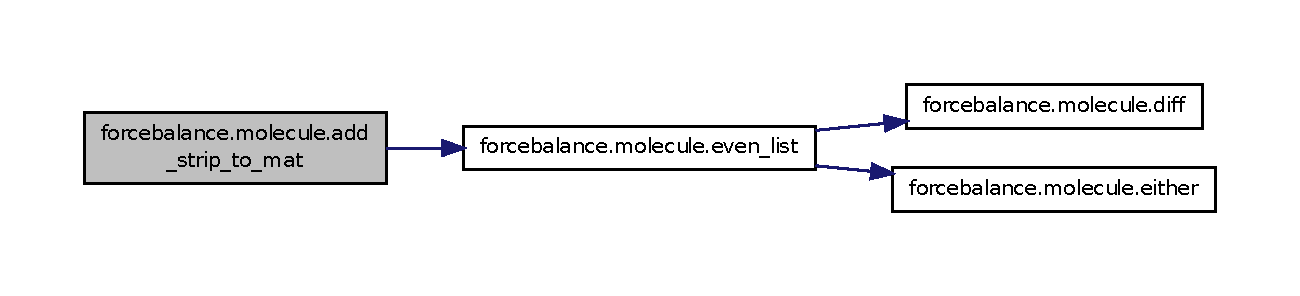
\includegraphics[width=350pt]{namespaceforcebalance_1_1molecule_a4cdb2086978b281ed84cd66179c3f5b2_cgraph}
\end{center}
\end{figure}


\hypertarget{namespaceforcebalance_1_1molecule_a9a58eb1746e51420f50da3f3a6d51485}{\index{forcebalance\-::molecule@{forcebalance\-::molecule}!Align\-To\-Density@{Align\-To\-Density}}
\index{Align\-To\-Density@{Align\-To\-Density}!forcebalance::molecule@{forcebalance\-::molecule}}
\paragraph[{Align\-To\-Density}]{\setlength{\rightskip}{0pt plus 5cm}def forcebalance.\-molecule.\-Align\-To\-Density (
\begin{DoxyParamCaption}
\item[{}]{elem, }
\item[{}]{xyz1, }
\item[{}]{xyz2, }
\item[{}]{binary = {\ttfamily False}}
\end{DoxyParamCaption}
)}}\label{namespaceforcebalance_1_1molecule_a9a58eb1746e51420f50da3f3a6d51485}


Computes a \char`\"{}overlap density\char`\"{} from two frames. 

This function can be called by Align\-To\-Moments to get rid of inversion problems 

Definition at line 541 of file molecule.\-py.



Here is the call graph for this function\-:\nopagebreak
\begin{figure}[H]
\begin{center}
\leavevmode
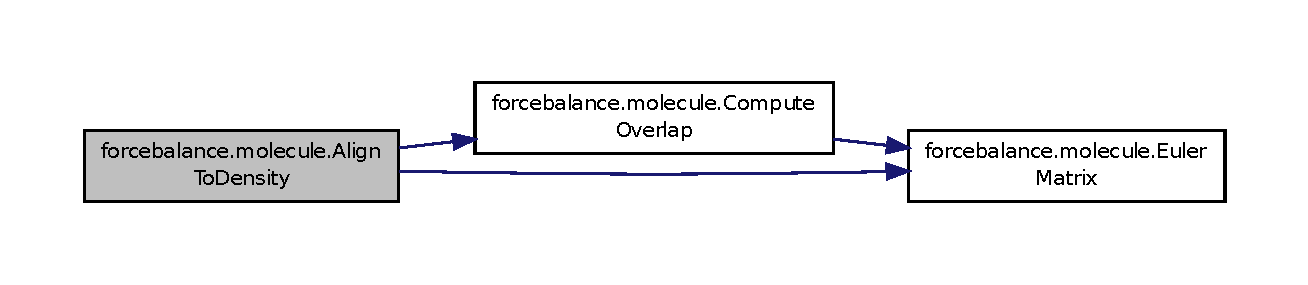
\includegraphics[width=350pt]{namespaceforcebalance_1_1molecule_a9a58eb1746e51420f50da3f3a6d51485_cgraph}
\end{center}
\end{figure}


\hypertarget{namespaceforcebalance_1_1molecule_aa9ad9b92efa7bd3c1d589d62bbb8108e}{\index{forcebalance\-::molecule@{forcebalance\-::molecule}!Align\-To\-Moments@{Align\-To\-Moments}}
\index{Align\-To\-Moments@{Align\-To\-Moments}!forcebalance::molecule@{forcebalance\-::molecule}}
\paragraph[{Align\-To\-Moments}]{\setlength{\rightskip}{0pt plus 5cm}def forcebalance.\-molecule.\-Align\-To\-Moments (
\begin{DoxyParamCaption}
\item[{}]{elem, }
\item[{}]{xyz1, }
\item[{}]{xyz2 = {\ttfamily None}}
\end{DoxyParamCaption}
)}}\label{namespaceforcebalance_1_1molecule_aa9ad9b92efa7bd3c1d589d62bbb8108e}


Pre-\/aligns molecules to 'moment of inertia'. 

If xyz2 is passed in, it will assume that xyz1 is already aligned to the moment of inertia, and it simply does 180-\/degree rotations to make sure nothing is inverted. 

Definition at line 553 of file molecule.\-py.

\hypertarget{namespaceforcebalance_1_1molecule_a5b50df23cc4d0e617fdc56538f0bea63}{\index{forcebalance\-::molecule@{forcebalance\-::molecule}!both@{both}}
\index{both@{both}!forcebalance::molecule@{forcebalance\-::molecule}}
\paragraph[{both}]{\setlength{\rightskip}{0pt plus 5cm}def forcebalance.\-molecule.\-both (
\begin{DoxyParamCaption}
\item[{}]{A, }
\item[{}]{B, }
\item[{}]{key}
\end{DoxyParamCaption}
)}}\label{namespaceforcebalance_1_1molecule_a5b50df23cc4d0e617fdc56538f0bea63}


Definition at line 476 of file molecule.\-py.

\hypertarget{namespaceforcebalance_1_1molecule_a0a6e3e79b04534bf2e83d09def189444}{\index{forcebalance\-::molecule@{forcebalance\-::molecule}!Build\-Lattice\-From\-Lengths\-Angles@{Build\-Lattice\-From\-Lengths\-Angles}}
\index{Build\-Lattice\-From\-Lengths\-Angles@{Build\-Lattice\-From\-Lengths\-Angles}!forcebalance::molecule@{forcebalance\-::molecule}}
\paragraph[{Build\-Lattice\-From\-Lengths\-Angles}]{\setlength{\rightskip}{0pt plus 5cm}def forcebalance.\-molecule.\-Build\-Lattice\-From\-Lengths\-Angles (
\begin{DoxyParamCaption}
\item[{}]{a, }
\item[{}]{b, }
\item[{}]{c, }
\item[{}]{alpha, }
\item[{}]{beta, }
\item[{}]{gamma}
\end{DoxyParamCaption}
)}}\label{namespaceforcebalance_1_1molecule_a0a6e3e79b04534bf2e83d09def189444}


This function takes in three lattice lengths and three lattice angles, and tries to return a complete box specification. 



Definition at line 258 of file molecule.\-py.



Here is the call graph for this function\-:\nopagebreak
\begin{figure}[H]
\begin{center}
\leavevmode
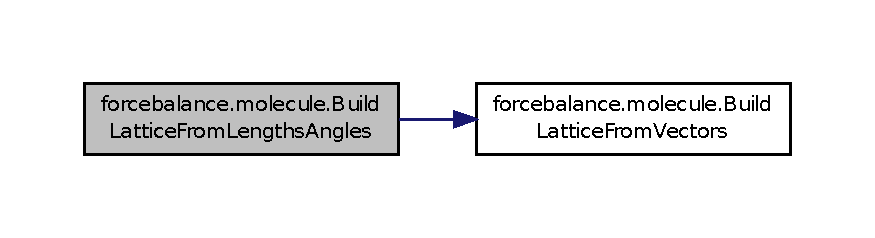
\includegraphics[width=350pt]{namespaceforcebalance_1_1molecule_a0a6e3e79b04534bf2e83d09def189444_cgraph}
\end{center}
\end{figure}


\hypertarget{namespaceforcebalance_1_1molecule_a29fb1ac9324f4280f07c65baea339989}{\index{forcebalance\-::molecule@{forcebalance\-::molecule}!Build\-Lattice\-From\-Vectors@{Build\-Lattice\-From\-Vectors}}
\index{Build\-Lattice\-From\-Vectors@{Build\-Lattice\-From\-Vectors}!forcebalance::molecule@{forcebalance\-::molecule}}
\paragraph[{Build\-Lattice\-From\-Vectors}]{\setlength{\rightskip}{0pt plus 5cm}def forcebalance.\-molecule.\-Build\-Lattice\-From\-Vectors (
\begin{DoxyParamCaption}
\item[{}]{v1, }
\item[{}]{v2, }
\item[{}]{v3}
\end{DoxyParamCaption}
)}}\label{namespaceforcebalance_1_1molecule_a29fb1ac9324f4280f07c65baea339989}


This function takes in three lattice vectors and tries to return a complete box specification. 

The hash function is something we can use to discard two things that are obviously not equal. Here we neglect the hash. Return a list of the sorted atom numbers in this graph. Return a string of atoms, which serves as a rudimentary 'fingerprint' \-: '99,100,103,151' . Return an array of the elements. For instance \mbox{[}'H' 'C' 'C' 'H'\mbox{]}. Create an Empirical Formula Get a list of the coordinates. 

Definition at line 273 of file molecule.\-py.

\hypertarget{namespaceforcebalance_1_1molecule_a8fcbb4a2b3470a85d25699b6f28a54fc}{\index{forcebalance\-::molecule@{forcebalance\-::molecule}!Compute\-Overlap@{Compute\-Overlap}}
\index{Compute\-Overlap@{Compute\-Overlap}!forcebalance::molecule@{forcebalance\-::molecule}}
\paragraph[{Compute\-Overlap}]{\setlength{\rightskip}{0pt plus 5cm}def forcebalance.\-molecule.\-Compute\-Overlap (
\begin{DoxyParamCaption}
\item[{}]{theta, }
\item[{}]{elem, }
\item[{}]{xyz1, }
\item[{}]{xyz2}
\end{DoxyParamCaption}
)}}\label{namespaceforcebalance_1_1molecule_a8fcbb4a2b3470a85d25699b6f28a54fc}


Computes an 'overlap' between two molecules based on some fictitious density. 

Good for fine-\/tuning alignment but gets stuck in local minima. 

Definition at line 524 of file molecule.\-py.



Here is the call graph for this function\-:\nopagebreak
\begin{figure}[H]
\begin{center}
\leavevmode
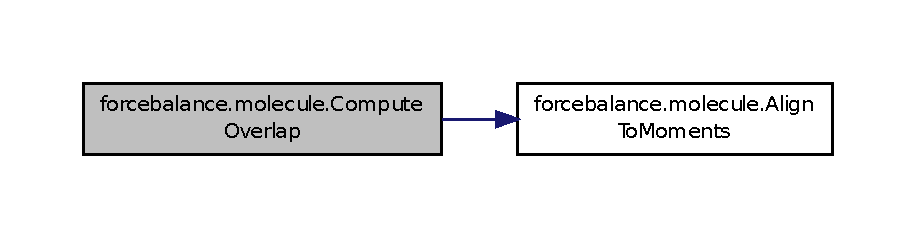
\includegraphics[width=350pt]{namespaceforcebalance_1_1molecule_a8fcbb4a2b3470a85d25699b6f28a54fc_cgraph}
\end{center}
\end{figure}


\hypertarget{namespaceforcebalance_1_1molecule_a6f7c6217b1c64da309a8abd21dfdcf08}{\index{forcebalance\-::molecule@{forcebalance\-::molecule}!diff@{diff}}
\index{diff@{diff}!forcebalance::molecule@{forcebalance\-::molecule}}
\paragraph[{diff}]{\setlength{\rightskip}{0pt plus 5cm}def forcebalance.\-molecule.\-diff (
\begin{DoxyParamCaption}
\item[{}]{A, }
\item[{}]{B, }
\item[{}]{key}
\end{DoxyParamCaption}
)}}\label{namespaceforcebalance_1_1molecule_a6f7c6217b1c64da309a8abd21dfdcf08}


Definition at line 479 of file molecule.\-py.

\hypertarget{namespaceforcebalance_1_1molecule_a75775be6563ad7f10695a9a45ff49ba9}{\index{forcebalance\-::molecule@{forcebalance\-::molecule}!either@{either}}
\index{either@{either}!forcebalance::molecule@{forcebalance\-::molecule}}
\paragraph[{either}]{\setlength{\rightskip}{0pt plus 5cm}def forcebalance.\-molecule.\-either (
\begin{DoxyParamCaption}
\item[{}]{A, }
\item[{}]{B, }
\item[{}]{key}
\end{DoxyParamCaption}
)}}\label{namespaceforcebalance_1_1molecule_a75775be6563ad7f10695a9a45ff49ba9}


Definition at line 487 of file molecule.\-py.

\hypertarget{namespaceforcebalance_1_1molecule_af02bf73765f34bbef81c4a5b000b86ce}{\index{forcebalance\-::molecule@{forcebalance\-::molecule}!Euler\-Matrix@{Euler\-Matrix}}
\index{Euler\-Matrix@{Euler\-Matrix}!forcebalance::molecule@{forcebalance\-::molecule}}
\paragraph[{Euler\-Matrix}]{\setlength{\rightskip}{0pt plus 5cm}def forcebalance.\-molecule.\-Euler\-Matrix (
\begin{DoxyParamCaption}
\item[{}]{T1, }
\item[{}]{T2, }
\item[{}]{T3}
\end{DoxyParamCaption}
)}}\label{namespaceforcebalance_1_1molecule_af02bf73765f34bbef81c4a5b000b86ce}


Constructs an Euler matrix from three Euler angles. 



Definition at line 496 of file molecule.\-py.



Here is the call graph for this function\-:\nopagebreak
\begin{figure}[H]
\begin{center}
\leavevmode
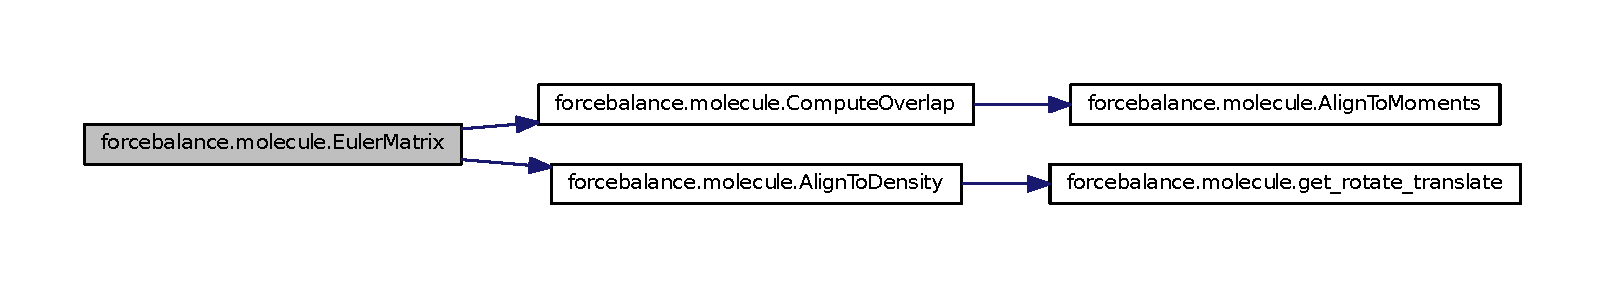
\includegraphics[width=350pt]{namespaceforcebalance_1_1molecule_af02bf73765f34bbef81c4a5b000b86ce_cgraph}
\end{center}
\end{figure}


\hypertarget{namespaceforcebalance_1_1molecule_a5f529179461765fadbd0a742cdc2c677}{\index{forcebalance\-::molecule@{forcebalance\-::molecule}!even\-\_\-list@{even\-\_\-list}}
\index{even\-\_\-list@{even\-\_\-list}!forcebalance::molecule@{forcebalance\-::molecule}}
\paragraph[{even\-\_\-list}]{\setlength{\rightskip}{0pt plus 5cm}def forcebalance.\-molecule.\-even\-\_\-list (
\begin{DoxyParamCaption}
\item[{}]{totlen, }
\item[{}]{splitsize}
\end{DoxyParamCaption}
)}}\label{namespaceforcebalance_1_1molecule_a5f529179461765fadbd0a742cdc2c677}


Creates a list of number sequences divided as evenly as possible. 



Definition at line 458 of file molecule.\-py.



Here is the call graph for this function\-:\nopagebreak
\begin{figure}[H]
\begin{center}
\leavevmode
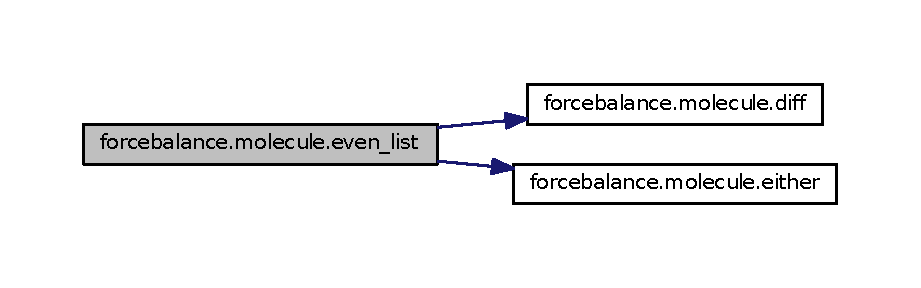
\includegraphics[width=350pt]{namespaceforcebalance_1_1molecule_a5f529179461765fadbd0a742cdc2c677_cgraph}
\end{center}
\end{figure}


\hypertarget{namespaceforcebalance_1_1molecule_ae25aa5331b3a2dd0e9d1e184380357db}{\index{forcebalance\-::molecule@{forcebalance\-::molecule}!format\-\_\-gro\-\_\-box@{format\-\_\-gro\-\_\-box}}
\index{format\-\_\-gro\-\_\-box@{format\-\_\-gro\-\_\-box}!forcebalance::molecule@{forcebalance\-::molecule}}
\paragraph[{format\-\_\-gro\-\_\-box}]{\setlength{\rightskip}{0pt plus 5cm}def forcebalance.\-molecule.\-format\-\_\-gro\-\_\-box (
\begin{DoxyParamCaption}
\item[{}]{box}
\end{DoxyParamCaption}
)}}\label{namespaceforcebalance_1_1molecule_ae25aa5331b3a2dd0e9d1e184380357db}


Print a line corresponding to the box vector in accordance with .gro file format. 


\begin{DoxyParams}[1]{Parameters}
\mbox{\tt in}  & {\em box} & Box Named\-Tuple \\
\hline
\end{DoxyParams}


Definition at line 389 of file molecule.\-py.



Here is the call graph for this function\-:\nopagebreak
\begin{figure}[H]
\begin{center}
\leavevmode
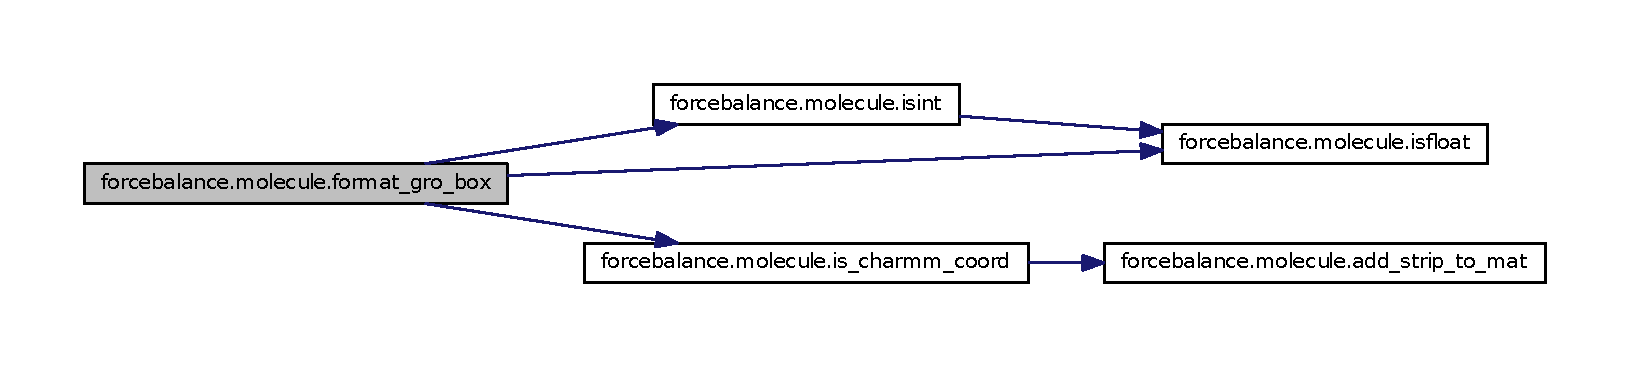
\includegraphics[width=350pt]{namespaceforcebalance_1_1molecule_ae25aa5331b3a2dd0e9d1e184380357db_cgraph}
\end{center}
\end{figure}


\hypertarget{namespaceforcebalance_1_1molecule_a41c13064e4285973aa6c49369d3d3390}{\index{forcebalance\-::molecule@{forcebalance\-::molecule}!format\-\_\-gro\-\_\-coord@{format\-\_\-gro\-\_\-coord}}
\index{format\-\_\-gro\-\_\-coord@{format\-\_\-gro\-\_\-coord}!forcebalance::molecule@{forcebalance\-::molecule}}
\paragraph[{format\-\_\-gro\-\_\-coord}]{\setlength{\rightskip}{0pt plus 5cm}def forcebalance.\-molecule.\-format\-\_\-gro\-\_\-coord (
\begin{DoxyParamCaption}
\item[{}]{resid, }
\item[{}]{resname, }
\item[{}]{aname, }
\item[{}]{seqno, }
\item[{}]{xyz}
\end{DoxyParamCaption}
)}}\label{namespaceforcebalance_1_1molecule_a41c13064e4285973aa6c49369d3d3390}


Print a line in accordance with .gro file format, with six decimal points of precision. 


\begin{DoxyParams}[1]{Parameters}
\mbox{\tt in}  & {\em resid} & The number of the residue that the atom belongs to \\
\hline
\mbox{\tt in}  & {\em resname} & The name of the residue that the atom belongs to \\
\hline
\mbox{\tt in}  & {\em aname} & The name of the atom \\
\hline
\mbox{\tt in}  & {\em seqno} & The sequential number of the atom \\
\hline
\mbox{\tt in}  & {\em xyz} & A 3-\/element array containing x, y, z coordinates of that atom \\
\hline
\end{DoxyParams}


Definition at line 368 of file molecule.\-py.



Here is the call graph for this function\-:\nopagebreak
\begin{figure}[H]
\begin{center}
\leavevmode
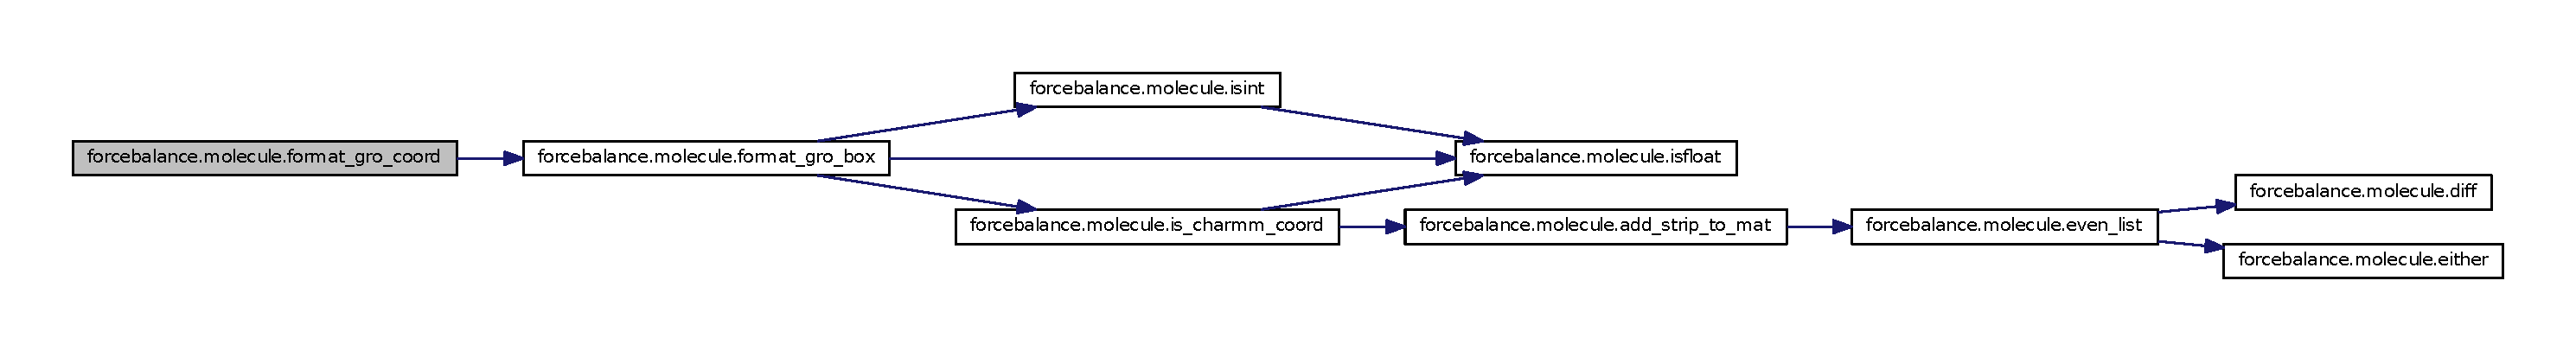
\includegraphics[width=350pt]{namespaceforcebalance_1_1molecule_a41c13064e4285973aa6c49369d3d3390_cgraph}
\end{center}
\end{figure}


\hypertarget{namespaceforcebalance_1_1molecule_a2eba3cad44138b3b10ea883240888412}{\index{forcebalance\-::molecule@{forcebalance\-::molecule}!format\-\_\-xyz\-\_\-coord@{format\-\_\-xyz\-\_\-coord}}
\index{format\-\_\-xyz\-\_\-coord@{format\-\_\-xyz\-\_\-coord}!forcebalance::molecule@{forcebalance\-::molecule}}
\paragraph[{format\-\_\-xyz\-\_\-coord}]{\setlength{\rightskip}{0pt plus 5cm}def forcebalance.\-molecule.\-format\-\_\-xyz\-\_\-coord (
\begin{DoxyParamCaption}
\item[{}]{element, }
\item[{}]{xyz, }
\item[{}]{tinker = {\ttfamily False}}
\end{DoxyParamCaption}
)}}\label{namespaceforcebalance_1_1molecule_a2eba3cad44138b3b10ea883240888412}


Print a line consisting of (element, x, y, z) in accordance with .xyz file format. 


\begin{DoxyParams}[1]{Parameters}
\mbox{\tt in}  & {\em element} & A chemical element of a single atom \\
\hline
\mbox{\tt in}  & {\em xyz} & A 3-\/element array containing x, y, z coordinates of that atom \\
\hline
\end{DoxyParams}


Definition at line 352 of file molecule.\-py.



Here is the call graph for this function\-:\nopagebreak
\begin{figure}[H]
\begin{center}
\leavevmode
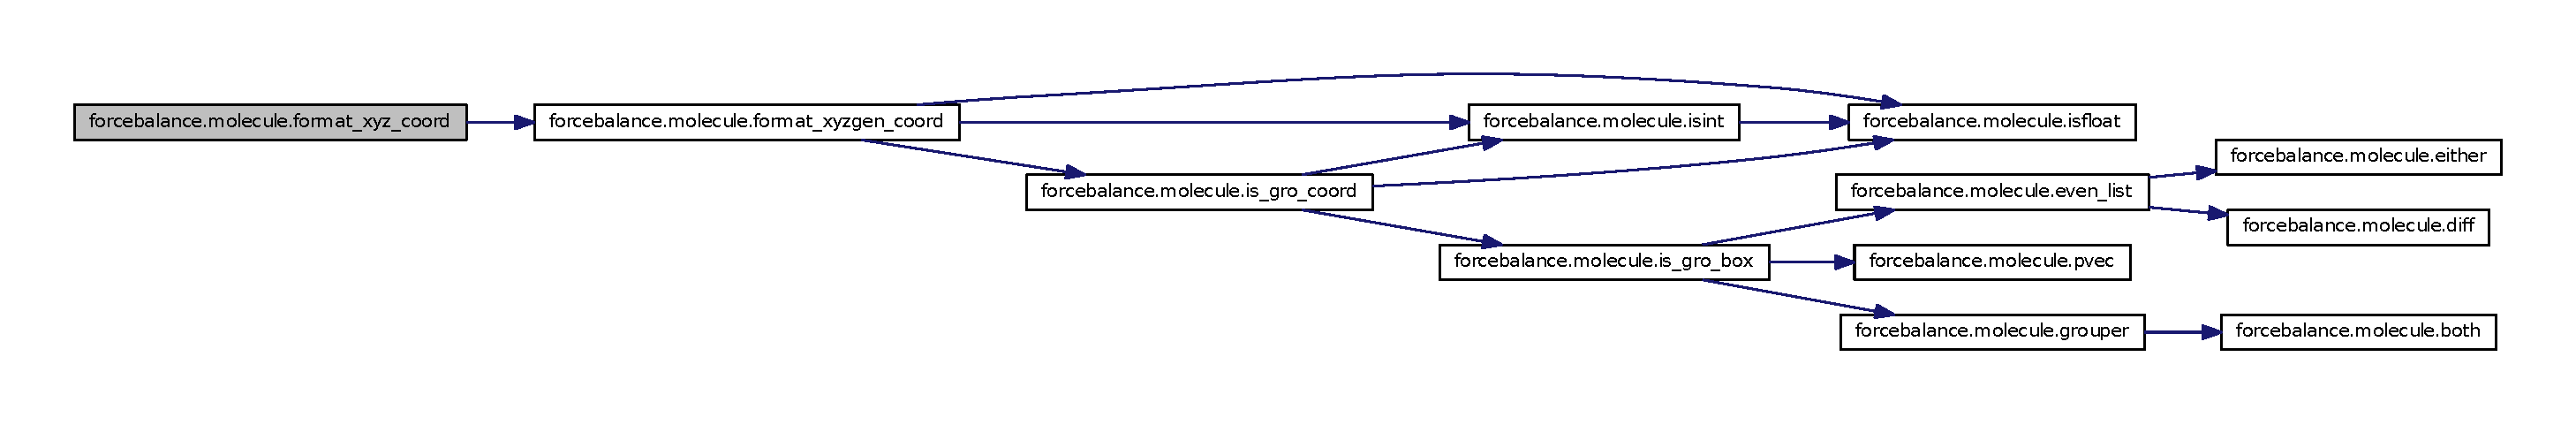
\includegraphics[width=350pt]{namespaceforcebalance_1_1molecule_a2eba3cad44138b3b10ea883240888412_cgraph}
\end{center}
\end{figure}


\hypertarget{namespaceforcebalance_1_1molecule_a4948e4662b8d2c8d515427d1bbb3d01e}{\index{forcebalance\-::molecule@{forcebalance\-::molecule}!format\-\_\-xyzgen\-\_\-coord@{format\-\_\-xyzgen\-\_\-coord}}
\index{format\-\_\-xyzgen\-\_\-coord@{format\-\_\-xyzgen\-\_\-coord}!forcebalance::molecule@{forcebalance\-::molecule}}
\paragraph[{format\-\_\-xyzgen\-\_\-coord}]{\setlength{\rightskip}{0pt plus 5cm}def forcebalance.\-molecule.\-format\-\_\-xyzgen\-\_\-coord (
\begin{DoxyParamCaption}
\item[{}]{element, }
\item[{}]{xyzgen}
\end{DoxyParamCaption}
)}}\label{namespaceforcebalance_1_1molecule_a4948e4662b8d2c8d515427d1bbb3d01e}


Print a line consisting of (element, p, q, r, s, t, ...) where (p, q, r) are arbitrary atom-\/wise data (this might happen, for instance, with atomic charges) 


\begin{DoxyParams}[1]{Parameters}
\mbox{\tt in}  & {\em element} & A chemical element of a single atom \\
\hline
\mbox{\tt in}  & {\em xyzgen} & A N-\/element array containing data for that atom \\
\hline
\end{DoxyParams}


Definition at line 380 of file molecule.\-py.



Here is the call graph for this function\-:\nopagebreak
\begin{figure}[H]
\begin{center}
\leavevmode
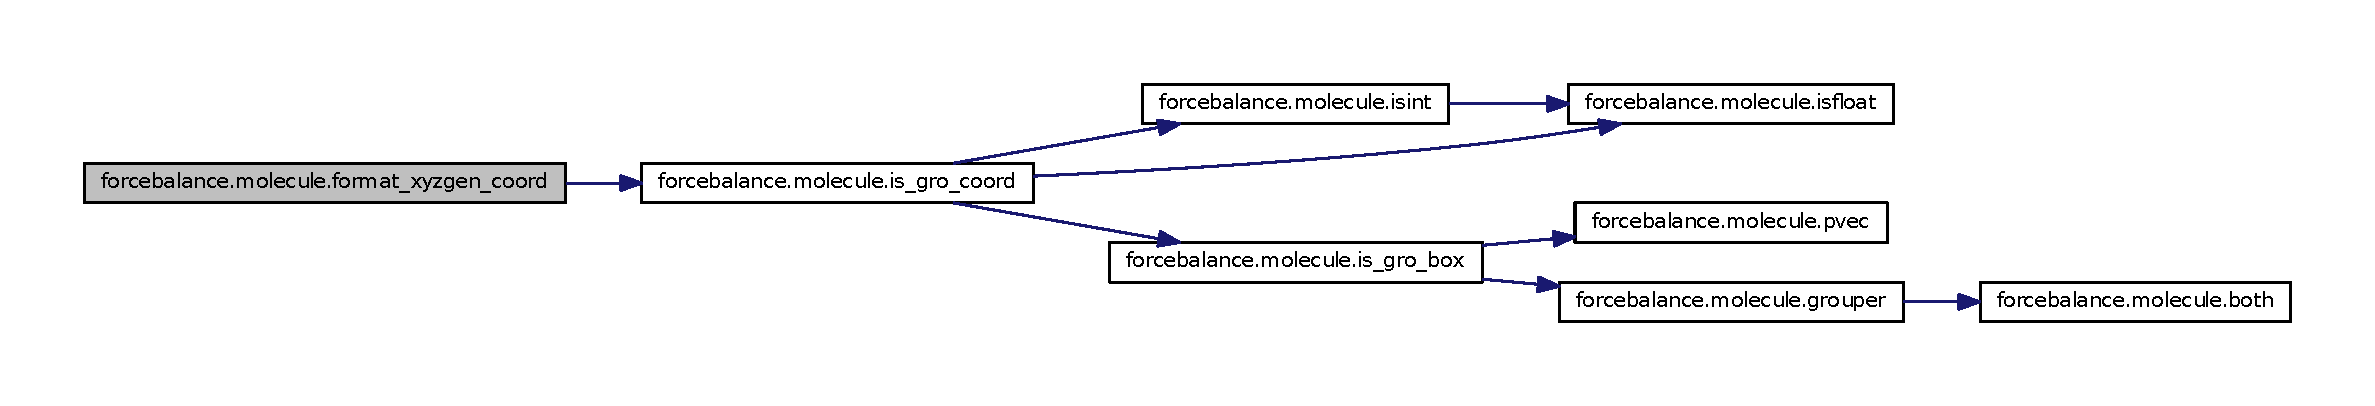
\includegraphics[width=350pt]{namespaceforcebalance_1_1molecule_a4948e4662b8d2c8d515427d1bbb3d01e_cgraph}
\end{center}
\end{figure}


\hypertarget{namespaceforcebalance_1_1molecule_a08840b73e95bf34bf9ca7ea36ad0492d}{\index{forcebalance\-::molecule@{forcebalance\-::molecule}!get\-\_\-rotate\-\_\-translate@{get\-\_\-rotate\-\_\-translate}}
\index{get\-\_\-rotate\-\_\-translate@{get\-\_\-rotate\-\_\-translate}!forcebalance::molecule@{forcebalance\-::molecule}}
\paragraph[{get\-\_\-rotate\-\_\-translate}]{\setlength{\rightskip}{0pt plus 5cm}def forcebalance.\-molecule.\-get\-\_\-rotate\-\_\-translate (
\begin{DoxyParamCaption}
\item[{}]{matrix1, }
\item[{}]{matrix2}
\end{DoxyParamCaption}
)}}\label{namespaceforcebalance_1_1molecule_a08840b73e95bf34bf9ca7ea36ad0492d}


Definition at line 576 of file molecule.\-py.

\hypertarget{namespaceforcebalance_1_1molecule_af28de4693e5b8e82df900d0ac3c6c370}{\index{forcebalance\-::molecule@{forcebalance\-::molecule}!get\-Element@{get\-Element}}
\index{get\-Element@{get\-Element}!forcebalance::molecule@{forcebalance\-::molecule}}
\paragraph[{get\-Element}]{\setlength{\rightskip}{0pt plus 5cm}def forcebalance.\-molecule.\-get\-Element (
\begin{DoxyParamCaption}
\item[{}]{mass}
\end{DoxyParamCaption}
)}}\label{namespaceforcebalance_1_1molecule_af28de4693e5b8e82df900d0ac3c6c370}


Definition at line 191 of file molecule.\-py.

\hypertarget{namespaceforcebalance_1_1molecule_a7fe52c2928c7b0329882541bef2e34cd}{\index{forcebalance\-::molecule@{forcebalance\-::molecule}!grouper@{grouper}}
\index{grouper@{grouper}!forcebalance::molecule@{forcebalance\-::molecule}}
\paragraph[{grouper}]{\setlength{\rightskip}{0pt plus 5cm}def forcebalance.\-molecule.\-grouper (
\begin{DoxyParamCaption}
\item[{}]{n, }
\item[{}]{iterable}
\end{DoxyParamCaption}
)}}\label{namespaceforcebalance_1_1molecule_a7fe52c2928c7b0329882541bef2e34cd}


Groups a big long iterable into groups of ten or what have you. 



Definition at line 452 of file molecule.\-py.



Here is the call graph for this function\-:\nopagebreak
\begin{figure}[H]
\begin{center}
\leavevmode
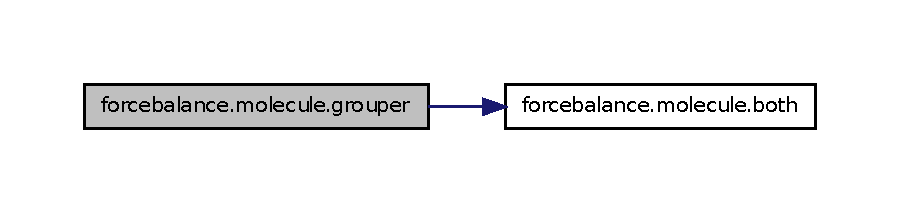
\includegraphics[width=350pt]{namespaceforcebalance_1_1molecule_a7fe52c2928c7b0329882541bef2e34cd_cgraph}
\end{center}
\end{figure}


\hypertarget{namespaceforcebalance_1_1molecule_a838d85848bd817e801d0f5f6502217ef}{\index{forcebalance\-::molecule@{forcebalance\-::molecule}!is\-\_\-charmm\-\_\-coord@{is\-\_\-charmm\-\_\-coord}}
\index{is\-\_\-charmm\-\_\-coord@{is\-\_\-charmm\-\_\-coord}!forcebalance::molecule@{forcebalance\-::molecule}}
\paragraph[{is\-\_\-charmm\-\_\-coord}]{\setlength{\rightskip}{0pt plus 5cm}def forcebalance.\-molecule.\-is\-\_\-charmm\-\_\-coord (
\begin{DoxyParamCaption}
\item[{}]{line}
\end{DoxyParamCaption}
)}}\label{namespaceforcebalance_1_1molecule_a838d85848bd817e801d0f5f6502217ef}


Determines whether a line contains C\-H\-A\-R\-M\-M data or not. 


\begin{DoxyParams}[1]{Parameters}
\mbox{\tt in}  & {\em line} & The line to be tested \\
\hline
\end{DoxyParams}


Definition at line 416 of file molecule.\-py.



Here is the call graph for this function\-:\nopagebreak
\begin{figure}[H]
\begin{center}
\leavevmode
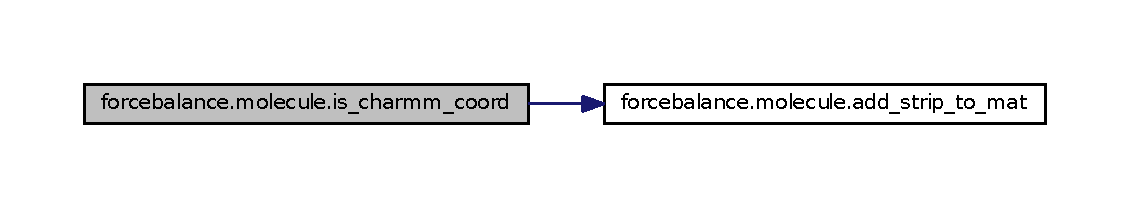
\includegraphics[width=350pt]{namespaceforcebalance_1_1molecule_a838d85848bd817e801d0f5f6502217ef_cgraph}
\end{center}
\end{figure}


\hypertarget{namespaceforcebalance_1_1molecule_aafc8c924eed4480fed8ddc9c474d3bc1}{\index{forcebalance\-::molecule@{forcebalance\-::molecule}!is\-\_\-gro\-\_\-box@{is\-\_\-gro\-\_\-box}}
\index{is\-\_\-gro\-\_\-box@{is\-\_\-gro\-\_\-box}!forcebalance::molecule@{forcebalance\-::molecule}}
\paragraph[{is\-\_\-gro\-\_\-box}]{\setlength{\rightskip}{0pt plus 5cm}def forcebalance.\-molecule.\-is\-\_\-gro\-\_\-box (
\begin{DoxyParamCaption}
\item[{}]{line}
\end{DoxyParamCaption}
)}}\label{namespaceforcebalance_1_1molecule_aafc8c924eed4480fed8ddc9c474d3bc1}


Determines whether a line contains a G\-R\-O\-M\-A\-C\-S box vector or not. 


\begin{DoxyParams}[1]{Parameters}
\mbox{\tt in}  & {\em line} & The line to be tested \\
\hline
\end{DoxyParams}


Definition at line 429 of file molecule.\-py.



Here is the call graph for this function\-:\nopagebreak
\begin{figure}[H]
\begin{center}
\leavevmode
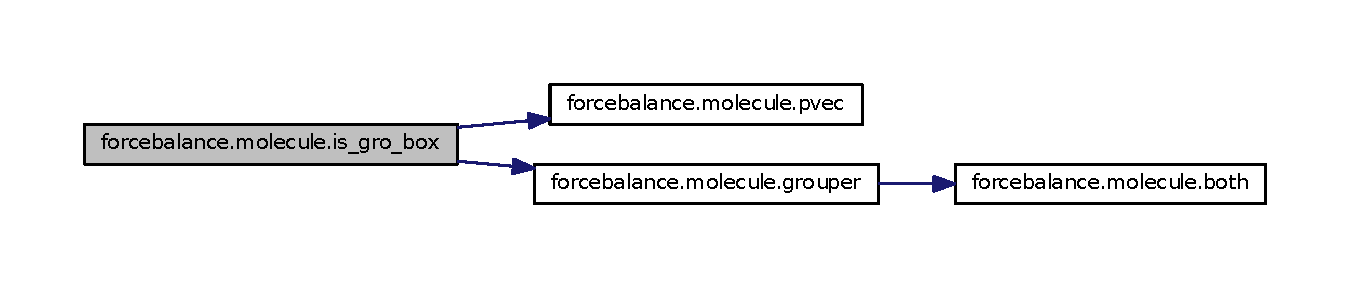
\includegraphics[width=350pt]{namespaceforcebalance_1_1molecule_aafc8c924eed4480fed8ddc9c474d3bc1_cgraph}
\end{center}
\end{figure}


\hypertarget{namespaceforcebalance_1_1molecule_a12b7bb398c2fa49a223f258ec7737483}{\index{forcebalance\-::molecule@{forcebalance\-::molecule}!is\-\_\-gro\-\_\-coord@{is\-\_\-gro\-\_\-coord}}
\index{is\-\_\-gro\-\_\-coord@{is\-\_\-gro\-\_\-coord}!forcebalance::molecule@{forcebalance\-::molecule}}
\paragraph[{is\-\_\-gro\-\_\-coord}]{\setlength{\rightskip}{0pt plus 5cm}def forcebalance.\-molecule.\-is\-\_\-gro\-\_\-coord (
\begin{DoxyParamCaption}
\item[{}]{line}
\end{DoxyParamCaption}
)}}\label{namespaceforcebalance_1_1molecule_a12b7bb398c2fa49a223f258ec7737483}


Determines whether a line contains G\-R\-O\-M\-A\-C\-S data or not. 


\begin{DoxyParams}[1]{Parameters}
\mbox{\tt in}  & {\em line} & The line to be tested \\
\hline
\end{DoxyParams}


Definition at line 401 of file molecule.\-py.



Here is the call graph for this function\-:\nopagebreak
\begin{figure}[H]
\begin{center}
\leavevmode
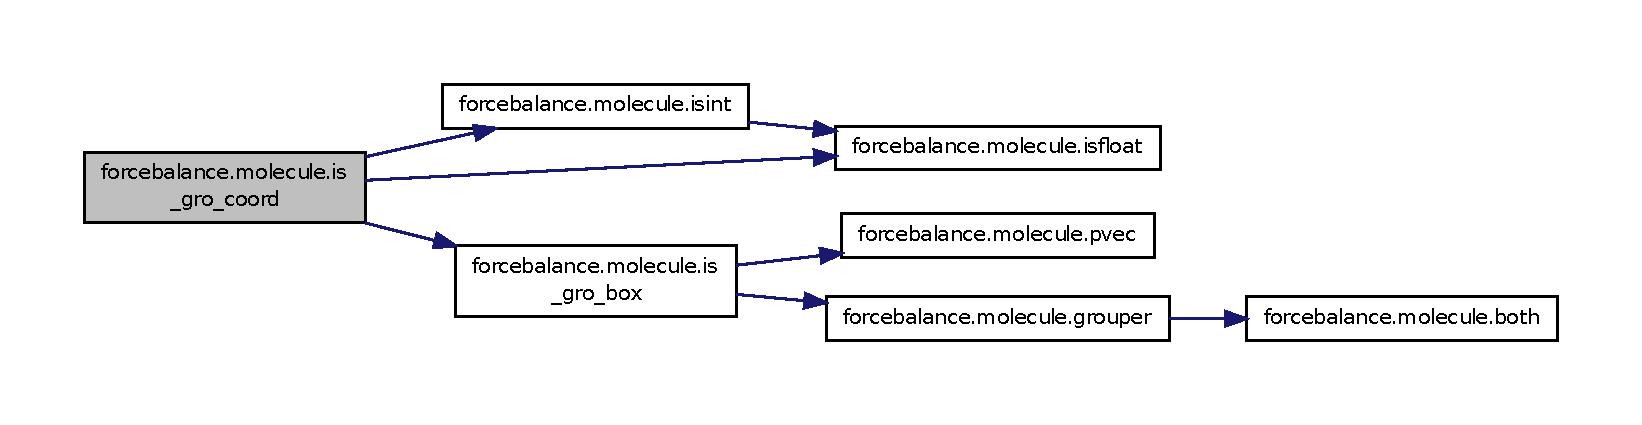
\includegraphics[width=350pt]{namespaceforcebalance_1_1molecule_a12b7bb398c2fa49a223f258ec7737483_cgraph}
\end{center}
\end{figure}


\hypertarget{namespaceforcebalance_1_1molecule_afe989ffd119568047fc8265b1d329a70}{\index{forcebalance\-::molecule@{forcebalance\-::molecule}!isfloat@{isfloat}}
\index{isfloat@{isfloat}!forcebalance::molecule@{forcebalance\-::molecule}}
\paragraph[{isfloat}]{\setlength{\rightskip}{0pt plus 5cm}def forcebalance.\-molecule.\-isfloat (
\begin{DoxyParamCaption}
\item[{}]{word}
\end{DoxyParamCaption}
)}}\label{namespaceforcebalance_1_1molecule_afe989ffd119568047fc8265b1d329a70}


Matches A\-N\-Y number; it can be a decimal, scientific notation, integer, or what have you. 



Definition at line 247 of file molecule.\-py.

\hypertarget{namespaceforcebalance_1_1molecule_a0dd31eff88d2bed0884ab21a13261d42}{\index{forcebalance\-::molecule@{forcebalance\-::molecule}!isint@{isint}}
\index{isint@{isint}!forcebalance::molecule@{forcebalance\-::molecule}}
\paragraph[{isint}]{\setlength{\rightskip}{0pt plus 5cm}def forcebalance.\-molecule.\-isint (
\begin{DoxyParamCaption}
\item[{}]{word}
\end{DoxyParamCaption}
)}}\label{namespaceforcebalance_1_1molecule_a0dd31eff88d2bed0884ab21a13261d42}


O\-N\-L\-Y matches integers! If you have a decimal point? None shall pass! 



Definition at line 242 of file molecule.\-py.



Here is the call graph for this function\-:\nopagebreak
\begin{figure}[H]
\begin{center}
\leavevmode
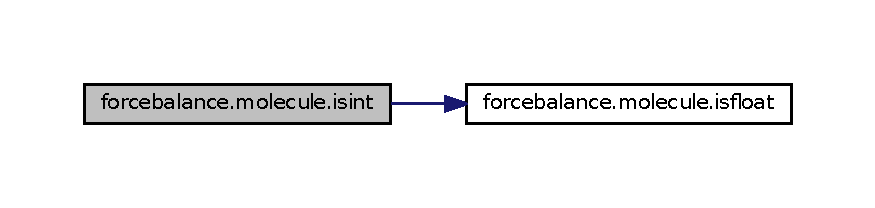
\includegraphics[width=350pt]{namespaceforcebalance_1_1molecule_a0dd31eff88d2bed0884ab21a13261d42_cgraph}
\end{center}
\end{figure}


\hypertarget{namespaceforcebalance_1_1molecule_ab9cb167fbbd809aedcf8c7434d405547}{\index{forcebalance\-::molecule@{forcebalance\-::molecule}!main@{main}}
\index{main@{main}!forcebalance::molecule@{forcebalance\-::molecule}}
\paragraph[{main}]{\setlength{\rightskip}{0pt plus 5cm}def forcebalance.\-molecule.\-main (
\begin{DoxyParamCaption}
{}
\end{DoxyParamCaption}
)}}\label{namespaceforcebalance_1_1molecule_ab9cb167fbbd809aedcf8c7434d405547}


Definition at line 2489 of file molecule.\-py.

\hypertarget{namespaceforcebalance_1_1molecule_ab8464fea13fad2a506792c2f1d7c93f3}{\index{forcebalance\-::molecule@{forcebalance\-::molecule}!nodematch@{nodematch}}
\index{nodematch@{nodematch}!forcebalance::molecule@{forcebalance\-::molecule}}
\paragraph[{nodematch}]{\setlength{\rightskip}{0pt plus 5cm}def forcebalance.\-molecule.\-nodematch (
\begin{DoxyParamCaption}
\item[{}]{node1, }
\item[{}]{node2}
\end{DoxyParamCaption}
)}}\label{namespaceforcebalance_1_1molecule_ab8464fea13fad2a506792c2f1d7c93f3}


Definition at line 236 of file molecule.\-py.



Here is the call graph for this function\-:\nopagebreak
\begin{figure}[H]
\begin{center}
\leavevmode
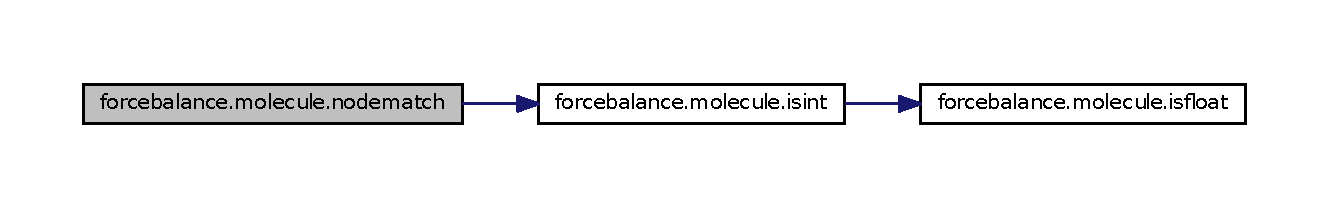
\includegraphics[width=350pt]{namespaceforcebalance_1_1molecule_ab8464fea13fad2a506792c2f1d7c93f3_cgraph}
\end{center}
\end{figure}


\hypertarget{namespaceforcebalance_1_1molecule_a58c3f09152db4d1c6e1db9df29c60c43}{\index{forcebalance\-::molecule@{forcebalance\-::molecule}!pvec@{pvec}}
\index{pvec@{pvec}!forcebalance::molecule@{forcebalance\-::molecule}}
\paragraph[{pvec}]{\setlength{\rightskip}{0pt plus 5cm}def forcebalance.\-molecule.\-pvec (
\begin{DoxyParamCaption}
\item[{}]{vec}
\end{DoxyParamCaption}
)}}\label{namespaceforcebalance_1_1molecule_a58c3f09152db4d1c6e1db9df29c60c43}


Definition at line 447 of file molecule.\-py.



\subsubsection{Variable Documentation}
\hypertarget{namespaceforcebalance_1_1molecule_a2986996d4f957928047df06fbec3717d}{\index{forcebalance\-::molecule@{forcebalance\-::molecule}!Alive@{Alive}}
\index{Alive@{Alive}!forcebalance::molecule@{forcebalance\-::molecule}}
\paragraph[{Alive}]{\setlength{\rightskip}{0pt plus 5cm}forcebalance.\-molecule.\-Alive}}\label{namespaceforcebalance_1_1molecule_a2986996d4f957928047df06fbec3717d}


Definition at line 302 of file molecule.\-py.

\hypertarget{namespaceforcebalance_1_1molecule_a8fcfb88fe12a9256b61980f3d4fe3b63}{\index{forcebalance\-::molecule@{forcebalance\-::molecule}!All\-Variable\-Names@{All\-Variable\-Names}}
\index{All\-Variable\-Names@{All\-Variable\-Names}!forcebalance::molecule@{forcebalance\-::molecule}}
\paragraph[{All\-Variable\-Names}]{\setlength{\rightskip}{0pt plus 5cm}forcebalance.\-molecule.\-All\-Variable\-Names = {\bf Quantum\-Variable\-Names}$|${\bf Atom\-Variable\-Names}$|${\bf Meta\-Variable\-Names}$|${\bf Frame\-Variable\-Names}}}\label{namespaceforcebalance_1_1molecule_a8fcfb88fe12a9256b61980f3d4fe3b63}


Definition at line 139 of file molecule.\-py.

\hypertarget{namespaceforcebalance_1_1molecule_a5daa68e835dcb9877d6c3f2fb559b54b}{\index{forcebalance\-::molecule@{forcebalance\-::molecule}!Atom\-Variable\-Names@{Atom\-Variable\-Names}}
\index{Atom\-Variable\-Names@{Atom\-Variable\-Names}!forcebalance::molecule@{forcebalance\-::molecule}}
\paragraph[{Atom\-Variable\-Names}]{\setlength{\rightskip}{0pt plus 5cm}tuple forcebalance.\-molecule.\-Atom\-Variable\-Names = set(\mbox{[}'elem', 'partial\-\_\-charge', 'atomname', 'atomtype', 'tinkersuf', 'resid', 'resname', 'qcsuf', 'qm\-\_\-ghost', 'chain', 'altloc', 'icode'\mbox{]})}}\label{namespaceforcebalance_1_1molecule_a5daa68e835dcb9877d6c3f2fb559b54b}


Definition at line 122 of file molecule.\-py.

\hypertarget{namespaceforcebalance_1_1molecule_a76af9edfbaaa8999680e32aafe1b1b61}{\index{forcebalance\-::molecule@{forcebalance\-::molecule}!bohrang@{bohrang}}
\index{bohrang@{bohrang}!forcebalance::molecule@{forcebalance\-::molecule}}
\paragraph[{bohrang}]{\setlength{\rightskip}{0pt plus 5cm}float forcebalance.\-molecule.\-bohrang = 0.\-529177249}}\label{namespaceforcebalance_1_1molecule_a76af9edfbaaa8999680e32aafe1b1b61}


One bohr equals this many angstroms. 



Definition at line 234 of file molecule.\-py.

\hypertarget{namespaceforcebalance_1_1molecule_aa761cf1cf260e15d0b03a6f61569c840}{\index{forcebalance\-::molecule@{forcebalance\-::molecule}!Box@{Box}}
\index{Box@{Box}!forcebalance::molecule@{forcebalance\-::molecule}}
\paragraph[{Box}]{\setlength{\rightskip}{0pt plus 5cm}tuple forcebalance.\-molecule.\-Box = namedtuple('Box',\mbox{[}'a','b','c','alpha','beta','gamma','A','B','C','V'\mbox{]})}}\label{namespaceforcebalance_1_1molecule_aa761cf1cf260e15d0b03a6f61569c840}


Definition at line 254 of file molecule.\-py.

\hypertarget{namespaceforcebalance_1_1molecule_a1c99a11e8a749468698c9af6361a8a4c}{\index{forcebalance\-::molecule@{forcebalance\-::molecule}!Elements@{Elements}}
\index{Elements@{Elements}!forcebalance::molecule@{forcebalance\-::molecule}}
\paragraph[{Elements}]{\setlength{\rightskip}{0pt plus 5cm}list forcebalance.\-molecule.\-Elements}}\label{namespaceforcebalance_1_1molecule_a1c99a11e8a749468698c9af6361a8a4c}
{\bfseries Initial value\-:}
\begin{DoxyCode}
1 = [\textcolor{stringliteral}{"None"},\textcolor{stringliteral}{'H'},\textcolor{stringliteral}{'He'},
2             \textcolor{stringliteral}{'Li'},\textcolor{stringliteral}{'Be'},\textcolor{stringliteral}{'B'},\textcolor{stringliteral}{'C'},\textcolor{stringliteral}{'N'},\textcolor{stringliteral}{'O'},\textcolor{stringliteral}{'F'},\textcolor{stringliteral}{'Ne'},
3             \textcolor{stringliteral}{'Na'},\textcolor{stringliteral}{'Mg'},\textcolor{stringliteral}{'Al'},\textcolor{stringliteral}{'Si'},\textcolor{stringliteral}{'P'},\textcolor{stringliteral}{'S'},\textcolor{stringliteral}{'Cl'},\textcolor{stringliteral}{'Ar'},
4             \textcolor{stringliteral}{'K'},\textcolor{stringliteral}{'Ca'},\textcolor{stringliteral}{'Sc'},\textcolor{stringliteral}{'Ti'},\textcolor{stringliteral}{'V'},\textcolor{stringliteral}{'Cr'},\textcolor{stringliteral}{'Mn'},\textcolor{stringliteral}{'Fe'},\textcolor{stringliteral}{'Co'},\textcolor{stringliteral}{'Ni'},\textcolor{stringliteral}{'Cu'},\textcolor{stringliteral}{'Zn'},\textcolor{stringliteral}{'Ga'},\textcolor{stringliteral}{'Ge'},\textcolor{stringliteral}{'As'},\textcolor{stringliteral}{'Se'},\textcolor{stringliteral}{'Br'},\textcolor{stringliteral}{'Kr'},
5             \textcolor{stringliteral}{'Rb'},\textcolor{stringliteral}{'Sr'},\textcolor{stringliteral}{'Y'},\textcolor{stringliteral}{'Zr'},\textcolor{stringliteral}{'Nb'},\textcolor{stringliteral}{'Mo'},\textcolor{stringliteral}{'Tc'},\textcolor{stringliteral}{'Ru'},\textcolor{stringliteral}{'Rh'},\textcolor{stringliteral}{'Pd'},\textcolor{stringliteral}{'Ag'},\textcolor{stringliteral}{'Cd'},\textcolor{stringliteral}{'In'},\textcolor{stringliteral}{'Sn'},\textcolor{stringliteral}{'Sb'},\textcolor{stringliteral}{'Te'},\textcolor{stringliteral}{'I'},\textcolor{stringliteral}{'Xe'},
6             \textcolor{stringliteral}{'Cs'},\textcolor{stringliteral}{'Ba'},\textcolor{stringliteral}{'La'},\textcolor{stringliteral}{'Ce'},\textcolor{stringliteral}{'Pr'},\textcolor{stringliteral}{'Nd'},\textcolor{stringliteral}{'Pm'},\textcolor{stringliteral}{'Sm'},\textcolor{stringliteral}{'Eu'},\textcolor{stringliteral}{'Gd'},\textcolor{stringliteral}{'Tb'},\textcolor{stringliteral}{'Dy'},\textcolor{stringliteral}{'Ho'},\textcolor{stringliteral}{'Er'},\textcolor{stringliteral}{'Tm'},\textcolor{stringliteral}{'Yb'},
7             \textcolor{stringliteral}{'Lu'},\textcolor{stringliteral}{'Hf'},\textcolor{stringliteral}{'Ta'},\textcolor{stringliteral}{'W'},\textcolor{stringliteral}{'Re'},\textcolor{stringliteral}{'Os'},\textcolor{stringliteral}{'Ir'},\textcolor{stringliteral}{'Pt'},\textcolor{stringliteral}{'Au'},\textcolor{stringliteral}{'Hg'},\textcolor{stringliteral}{'Tl'},\textcolor{stringliteral}{'Pb'},\textcolor{stringliteral}{'Bi'},\textcolor{stringliteral}{'Po'},\textcolor{stringliteral}{'At'},\textcolor{stringliteral}{'Rn'},
8             \textcolor{stringliteral}{'Fr'},\textcolor{stringliteral}{'Ra'},\textcolor{stringliteral}{'Ac'},\textcolor{stringliteral}{'Th'},\textcolor{stringliteral}{'Pa'},\textcolor{stringliteral}{'}\textcolor{stringliteral}{U','}Np','Pu','Am','Cm','Bk','Cf','Es','Fm','Md','No','Lr','Rf','Db','
      Sg','Bh','Hs','Mt']
\end{DoxyCode}


Definition at line 166 of file molecule.\-py.

\hypertarget{namespaceforcebalance_1_1molecule_a0044fa397e0923635a8b3e9625aa70f7}{\index{forcebalance\-::molecule@{forcebalance\-::molecule}!Frame\-Variable\-Names@{Frame\-Variable\-Names}}
\index{Frame\-Variable\-Names@{Frame\-Variable\-Names}!forcebalance::molecule@{forcebalance\-::molecule}}
\paragraph[{Frame\-Variable\-Names}]{\setlength{\rightskip}{0pt plus 5cm}tuple forcebalance.\-molecule.\-Frame\-Variable\-Names}}\label{namespaceforcebalance_1_1molecule_a0044fa397e0923635a8b3e9625aa70f7}
{\bfseries Initial value\-:}
\begin{DoxyCode}
1 = set([\textcolor{stringliteral}{'xyzs'}, \textcolor{stringliteral}{'comms'}, \textcolor{stringliteral}{'boxes'}, \textcolor{stringliteral}{'qm\_forces'}, \textcolor{stringliteral}{'qm\_energies'}, \textcolor{stringliteral}{'qm\_interaction'}, 
2                           \textcolor{stringliteral}{'qm\_espxyzs'}, \textcolor{stringliteral}{'qm\_espvals'}, \textcolor{stringliteral}{'qm\_extchgs'}, \textcolor{stringliteral}{'qm\_mulliken\_charges'}, \textcolor{stringliteral}{'
      qm\_mulliken\_spins'}])
\end{DoxyCode}


Definition at line 108 of file molecule.\-py.

\hypertarget{namespaceforcebalance_1_1molecule_a38e1c99e9567fe42b792af43db9b7488}{\index{forcebalance\-::molecule@{forcebalance\-::molecule}!Meta\-Variable\-Names@{Meta\-Variable\-Names}}
\index{Meta\-Variable\-Names@{Meta\-Variable\-Names}!forcebalance::molecule@{forcebalance\-::molecule}}
\paragraph[{Meta\-Variable\-Names}]{\setlength{\rightskip}{0pt plus 5cm}tuple forcebalance.\-molecule.\-Meta\-Variable\-Names = set(\mbox{[}'fnm', 'ftype', 'qcrems', 'qctemplate', 'charge', 'mult', 'bonds'\mbox{]})}}\label{namespaceforcebalance_1_1molecule_a38e1c99e9567fe42b792af43db9b7488}


Definition at line 135 of file molecule.\-py.

\hypertarget{namespaceforcebalance_1_1molecule_adc5040ec456762f2ac240fb08febbfdd}{\index{forcebalance\-::molecule@{forcebalance\-::molecule}!Periodic\-Table@{Periodic\-Table}}
\index{Periodic\-Table@{Periodic\-Table}!forcebalance::molecule@{forcebalance\-::molecule}}
\paragraph[{Periodic\-Table}]{\setlength{\rightskip}{0pt plus 5cm}tuple forcebalance.\-molecule.\-Periodic\-Table}}\label{namespaceforcebalance_1_1molecule_adc5040ec456762f2ac240fb08febbfdd}
{\bfseries Initial value\-:}
\begin{DoxyCode}
1 = OrderedDict([(\textcolor{stringliteral}{'H'} , 1.0079), (\textcolor{stringliteral}{'He'} , 4.0026), 
2                              (\textcolor{stringliteral}{'Li'} , 6.941), (\textcolor{stringliteral}{'Be'} , 9.0122), (\textcolor{stringliteral}{'B'} , 10.811), (\textcolor{stringliteral}{'C'} , 12.0107), (\textcolor{stringliteral}{'N'} , 14.00
      67), (\textcolor{stringliteral}{'O'} , 15.9994), (\textcolor{stringliteral}{'F'} , 18.9984), (\textcolor{stringliteral}{'Ne'} , 20.1797),
3                              (\textcolor{stringliteral}{'Na'} , 22.9897), (\textcolor{stringliteral}{'Mg'} , 24.305), (\textcolor{stringliteral}{'Al'} , 26.9815), (\textcolor{stringliteral}{'Si'} , 28.0855), (\textcolor{stringliteral}{'P'} , 
      30.9738), (\textcolor{stringliteral}{'S'} , 32.065), (\textcolor{stringliteral}{'Cl'} , 35.453), (\textcolor{stringliteral}{'Ar'} , 39.948), 
4                              (\textcolor{stringliteral}{'K'} , 39.0983), (\textcolor{stringliteral}{'Ca'} , 40.078), (\textcolor{stringliteral}{'Sc'} , 44.9559), (\textcolor{stringliteral}{'Ti'} , 47.867), (\textcolor{stringliteral}{'V'} , 50
      .9415), (\textcolor{stringliteral}{'Cr'} , 51.9961), (\textcolor{stringliteral}{'Mn'} , 54.938), (\textcolor{stringliteral}{'Fe'} , 55.845), (\textcolor{stringliteral}{'Co'} , 58.9332), 
5                              (\textcolor{stringliteral}{'Ni'} , 58.6934), (\textcolor{stringliteral}{'Cu'} , 63.546), (\textcolor{stringliteral}{'Zn'} , 65.39), (\textcolor{stringliteral}{'Ga'} , 69.723), (\textcolor{stringliteral}{'Ge'} , 72
      .64), (\textcolor{stringliteral}{'As'} , 74.9216), (\textcolor{stringliteral}{'Se'} , 78.96), (\textcolor{stringliteral}{'Br'} , 79.904), (\textcolor{stringliteral}{'Kr'} , 83.8), 
6                              (\textcolor{stringliteral}{'Rb'} , 85.4678), (\textcolor{stringliteral}{'Sr'} , 87.62), (\textcolor{stringliteral}{'Y'} , 88.9059), (\textcolor{stringliteral}{'Zr'} , 91.224), (\textcolor{stringliteral}{'Nb'} , 92
      .9064), (\textcolor{stringliteral}{'Mo'} , 95.94), (\textcolor{stringliteral}{'Tc'} , 98), (\textcolor{stringliteral}{'Ru'} , 101.07), (\textcolor{stringliteral}{'Rh'} , 102.9055), 
7                              (\textcolor{stringliteral}{'Pd'} , 106.42), (\textcolor{stringliteral}{'Ag'} , 107.8682), (\textcolor{stringliteral}{'Cd'} , 112.411), (\textcolor{stringliteral}{'In'} , 114.818), (\textcolor{stringliteral}{'Sn'} 
      , 118.71), (\textcolor{stringliteral}{'Sb'} , 121.76), (\textcolor{stringliteral}{'Te'} , 127.6), (\textcolor{stringliteral}{'I'} , 126.9045), (\textcolor{stringliteral}{'Xe'} , 131.293), 
8                              (\textcolor{stringliteral}{'Cs'} , 132.9055), (\textcolor{stringliteral}{'Ba'} , 137.327), (\textcolor{stringliteral}{'La'} , 138.9055), (\textcolor{stringliteral}{'Ce'} , 140.116), (\textcolor{stringliteral}{'Pr
      '} , 140.9077), (\textcolor{stringliteral}{'Nd'} , 144.24), (\textcolor{stringliteral}{'Pm'} , 145), (\textcolor{stringliteral}{'Sm'} , 150.36), 
9                              (\textcolor{stringliteral}{'Eu'} , 151.964), (\textcolor{stringliteral}{'Gd'} , 157.25), (\textcolor{stringliteral}{'Tb'} , 158.9253), (\textcolor{stringliteral}{'Dy'} , 162.5), (\textcolor{stringliteral}{'Ho'} , 
      164.9303), (\textcolor{stringliteral}{'Er'} , 167.259), (\textcolor{stringliteral}{'Tm'} , 168.9342), (\textcolor{stringliteral}{'Yb'} , 173.04), 
10                              (\textcolor{stringliteral}{'Lu'} , 174.967), (\textcolor{stringliteral}{'Hf'} , 178.49), (\textcolor{stringliteral}{'Ta'} , 180.9479), (\textcolor{stringliteral}{'W'} , 183.84), (\textcolor{stringliteral}{'Re'} , 
      186.207), (\textcolor{stringliteral}{'Os'} , 190.23), (\textcolor{stringliteral}{'Ir'} , 192.217), (\textcolor{stringliteral}{'Pt'} , 195.078), 
11                              (\textcolor{stringliteral}{'Au'} , 196.9665), (\textcolor{stringliteral}{'Hg'} , 200.59), (\textcolor{stringliteral}{'Tl'} , 204.3833), (\textcolor{stringliteral}{'Pb'} , 207.2), (\textcolor{stringliteral}{'Bi'} ,
       208.9804), (\textcolor{stringliteral}{'Po'} , 209), (\textcolor{stringliteral}{'At'} , 210), (\textcolor{stringliteral}{'Rn'} , 222), 
12                              (\textcolor{stringliteral}{'Fr'} , 223), (\textcolor{stringliteral}{'Ra'} , 226), (\textcolor{stringliteral}{'Ac'} , 227), (\textcolor{stringliteral}{'Th'} , 232.0381), (\textcolor{stringliteral}{'Pa'} , 231.0359)
      , (\textcolor{stringliteral}{'}\textcolor{stringliteral}{U' , 238.0289), ('}Np' , 237), ('Pu' , 244), 
13                              (\textcolor{stringliteral}{'Am'} , 243), (\textcolor{stringliteral}{'Cm'} , 247), (\textcolor{stringliteral}{'Bk'} , 247), (\textcolor{stringliteral}{'Cf'} , 251), (\textcolor{stringliteral}{'Es'} , 252), (\textcolor{stringliteral}{'Fm'} , 
      257), (\textcolor{stringliteral}{'Md'} , 258), (\textcolor{stringliteral}{'No'} , 259), 
14                              (\textcolor{stringliteral}{'Lr'} , 262), (\textcolor{stringliteral}{'Rf'} , 261), (\textcolor{stringliteral}{'Db'} , 262), (\textcolor{stringliteral}{'Sg'} , 266), (\textcolor{stringliteral}{'Bh'} , 264), (\textcolor{stringliteral}{'Hs'} , 
      277), (\textcolor{stringliteral}{'Mt'} , 268)])
\end{DoxyCode}


Definition at line 176 of file molecule.\-py.

\hypertarget{namespaceforcebalance_1_1molecule_ab67efeab6049ec1f416b9ad1eed6ffcc}{\index{forcebalance\-::molecule@{forcebalance\-::molecule}!Quantum\-Variable\-Names@{Quantum\-Variable\-Names}}
\index{Quantum\-Variable\-Names@{Quantum\-Variable\-Names}!forcebalance::molecule@{forcebalance\-::molecule}}
\paragraph[{Quantum\-Variable\-Names}]{\setlength{\rightskip}{0pt plus 5cm}tuple forcebalance.\-molecule.\-Quantum\-Variable\-Names = set(\mbox{[}'qcrems', 'qctemplate', 'charge', 'mult', 'qcsuf', 'qm\-\_\-ghost'\mbox{]})}}\label{namespaceforcebalance_1_1molecule_ab67efeab6049ec1f416b9ad1eed6ffcc}


Definition at line 137 of file molecule.\-py.

\hypertarget{namespaceforcebalance_1_1molecule_a1ee5389ce8a9042e053c7972dbbfb005}{\index{forcebalance\-::molecule@{forcebalance\-::molecule}!radian@{radian}}
\index{radian@{radian}!forcebalance::molecule@{forcebalance\-::molecule}}
\paragraph[{radian}]{\setlength{\rightskip}{0pt plus 5cm}int forcebalance.\-molecule.\-radian = 180}}\label{namespaceforcebalance_1_1molecule_a1ee5389ce8a9042e053c7972dbbfb005}


Definition at line 255 of file molecule.\-py.

\hypertarget{namespaceforcebalance_1_1molecule_a74f55a89a14ca676b5a06441d1fdab19}{\index{forcebalance\-::molecule@{forcebalance\-::molecule}!Radii@{Radii}}
\index{Radii@{Radii}!forcebalance::molecule@{forcebalance\-::molecule}}
\paragraph[{Radii}]{\setlength{\rightskip}{0pt plus 5cm}list forcebalance.\-molecule.\-Radii}}\label{namespaceforcebalance_1_1molecule_a74f55a89a14ca676b5a06441d1fdab19}
{\bfseries Initial value\-:}
\begin{DoxyCode}
1 = [0.31, 0.28, \textcolor{comment}{# H and He}
2          1.28, 0.96, 0.84, 0.76, 0.71, 0.66, 0.57, 0.58, \textcolor{comment}{# First row elements}
3          1.66, 1.41, 1.21, 1.11, 1.07, 1.05, 1.02, 1.06, \textcolor{comment}{# Second row elements}
4          2.03, 1.76, 1.70, 1.60, 1.53, 1.39, 1.61, 1.52, 1.50, 
5          1.24, 1.32, 1.22, 1.22, 1.20, 1.19, 1.20, 1.20, 1.16, \textcolor{comment}{# Third row elements, K through Kr}
6          2.20, 1.95, 1.90, 1.75, 1.64, 1.54, 1.47, 1.46, 1.42, 
7          1.39, 1.45, 1.44, 1.42, 1.39, 1.39, 1.38, 1.39, 1.40, \textcolor{comment}{# Fourth row elements, Rb through Xe}
8          2.44, 2.15, 2.07, 2.04, 2.03, 2.01, 1.99, 1.98, 
9          1.98, 1.96, 1.94, 1.92, 1.92, 1.89, 1.90, 1.87, \textcolor{comment}{# Fifth row elements, s and f blocks}
10          1.87, 1.75, 1.70, 1.62, 1.51, 1.44, 1.41, 1.36, 
11          1.36, 1.32, 1.45, 1.46, 1.48, 1.40, 1.50, 1.50, \textcolor{comment}{# Fifth row elements, d and p blocks}
12          2.60, 2.21, 2.15, 2.06, 2.00, 1.96, 1.90, 1.87, 1.80, 1.69]
\end{DoxyCode}


Definition at line 152 of file molecule.\-py.

\hypertarget{namespaceforcebalance_1_1molecule_a09d04113accea9c88b084051c5de29d1}{\index{forcebalance\-::molecule@{forcebalance\-::molecule}!splitter@{splitter}}
\index{splitter@{splitter}!forcebalance::molecule@{forcebalance\-::molecule}}
\paragraph[{splitter}]{\setlength{\rightskip}{0pt plus 5cm}tuple forcebalance.\-molecule.\-splitter = re.\-compile(r'(\textbackslash{}s+$|$\textbackslash{}S+)')}}\label{namespaceforcebalance_1_1molecule_a09d04113accea9c88b084051c5de29d1}


Definition at line 251 of file molecule.\-py.


\hypertarget{namespaceforcebalance_1_1moments}{\subsection{forcebalance.\-moments Namespace Reference}
\label{namespaceforcebalance_1_1moments}\index{forcebalance.\-moments@{forcebalance.\-moments}}
}

\hypertarget{namespaceforcebalance_1_1nifty}{\subsection{forcebalance.\-nifty Namespace Reference}
\label{namespaceforcebalance_1_1nifty}\index{forcebalance.\-nifty@{forcebalance.\-nifty}}
}


Nifty functions, intended to be imported by any module within Force\-Balance.  


\subsubsection*{Classes}
\begin{DoxyCompactItemize}
\item 
class \hyperlink{classforcebalance_1_1nifty_1_1Pickler__LP}{Pickler\-\_\-\-L\-P}
\begin{DoxyCompactList}\small\item\em A subclass of the python Pickler that implements pickling of \-\_\-\-Element\-Tree types. \end{DoxyCompactList}\item 
class \hyperlink{classforcebalance_1_1nifty_1_1Unpickler__LP}{Unpickler\-\_\-\-L\-P}
\begin{DoxyCompactList}\small\item\em A subclass of the python Unpickler that implements unpickling of \-\_\-\-Element\-Tree types. \end{DoxyCompactList}\end{DoxyCompactItemize}
\subsubsection*{Functions}
\begin{DoxyCompactItemize}
\item 
def \hyperlink{namespaceforcebalance_1_1nifty_a27e3a9dc144a5ad505509ac9ede08d7d}{pvec1d}
\begin{DoxyCompactList}\small\item\em Printout of a 1-\/\-D vector. \end{DoxyCompactList}\item 
def \hyperlink{namespaceforcebalance_1_1nifty_af61d76c8eb78c8ee52a43e239ff26cb4}{pmat2d}
\begin{DoxyCompactList}\small\item\em Printout of a 2-\/\-D matrix. \end{DoxyCompactList}\item 
def \hyperlink{namespaceforcebalance_1_1nifty_a3b437964dc22735bf8a7dcbaf99e413d}{encode}
\item 
def \hyperlink{namespaceforcebalance_1_1nifty_a3b9fd8e29c5d8f1b2114e4d9662dfd61}{segments}
\item 
def \hyperlink{namespaceforcebalance_1_1nifty_a9628ee448710667747d8aa5dc166532c}{commadash}
\item 
def \hyperlink{namespaceforcebalance_1_1nifty_afa670d68f01813ac8d429bc5cbdb4f9f}{uncommadash}
\item 
def \hyperlink{namespaceforcebalance_1_1nifty_a11babd62dc7bca389162c6318f9672ca}{printcool}
\begin{DoxyCompactList}\small\item\em Cool-\/looking printout for slick formatting of output. \end{DoxyCompactList}\item 
def \hyperlink{namespaceforcebalance_1_1nifty_a51180e960742cc7547749fdfb3513ec4}{printcool\-\_\-dictionary}
\begin{DoxyCompactList}\small\item\em See documentation for printcool; this is a nice way to print out keys/values in a dictionary. \end{DoxyCompactList}\item 
def \hyperlink{namespaceforcebalance_1_1nifty_a3f1c7a1af9d35d5d1693074bc6f5497c}{isint}
\begin{DoxyCompactList}\small\item\em O\-N\-L\-Y matches integers! If you have a decimal point? None shall pass! \end{DoxyCompactList}\item 
def \hyperlink{namespaceforcebalance_1_1nifty_a8e3ef0108b9d37b82ba0dced7c6037ae}{isfloat}
\begin{DoxyCompactList}\small\item\em Matches A\-N\-Y number; it can be a decimal, scientific notation, what have you C\-A\-U\-T\-I\-O\-N -\/ this will also match an integer. \end{DoxyCompactList}\item 
def \hyperlink{namespaceforcebalance_1_1nifty_a09263927eaec9deff283fbf1a820242f}{isdecimal}
\begin{DoxyCompactList}\small\item\em Matches things with a decimal only; see isint and isfloat. \end{DoxyCompactList}\item 
def \hyperlink{namespaceforcebalance_1_1nifty_a8d63c8ae9a67c66673a6cf81357f827d}{floatornan}
\begin{DoxyCompactList}\small\item\em Returns a big number if we encounter Na\-N. \end{DoxyCompactList}\item 
def \hyperlink{namespaceforcebalance_1_1nifty_afb3f205bce4984856e766af7e9fdaca8}{col}
\begin{DoxyCompactList}\small\item\em Given any list, array, or matrix, return a 1-\/column matrix. \end{DoxyCompactList}\item 
def \hyperlink{namespaceforcebalance_1_1nifty_a6c9727360cdff8f3011a12cc54d0e86e}{row}
\begin{DoxyCompactList}\small\item\em Given any list, array, or matrix, return a 1-\/row matrix. \end{DoxyCompactList}\item 
def \hyperlink{namespaceforcebalance_1_1nifty_a52114ceee9d55f94d9aecb3e176de294}{flat}
\begin{DoxyCompactList}\small\item\em Given any list, array, or matrix, return a single-\/index array. \end{DoxyCompactList}\item 
def \hyperlink{namespaceforcebalance_1_1nifty_a7676236002c6a65ea7d2e69a09923889}{orthogonalize}
\begin{DoxyCompactList}\small\item\em Given two vectors vec1 and vec2, project out the component of vec1 that is along the vec2-\/direction. \end{DoxyCompactList}\item 
def \hyperlink{namespaceforcebalance_1_1nifty_a4c82187e92dfeb8a159f4aa44b501c40}{invert\-\_\-svd}
\begin{DoxyCompactList}\small\item\em Invert a matrix using singular value decomposition. \end{DoxyCompactList}\item 
def \hyperlink{namespaceforcebalance_1_1nifty_aa9fb9c7c65231eca50a7afc04f489b64}{get\-\_\-least\-\_\-squares}
\item 
def \hyperlink{namespaceforcebalance_1_1nifty_ad5ca60565c864b4245a8212fe9d92e10}{statistical\-Inefficiency}
\begin{DoxyCompactList}\small\item\em Compute the (cross) statistical inefficiency of (two) timeseries. \end{DoxyCompactList}\item 
def \hyperlink{namespaceforcebalance_1_1nifty_a2ff762a2f2d2b6bb1c7dd067bd1a1e88}{lp\-\_\-dump}
\begin{DoxyCompactList}\small\item\em Use this instead of pickle.\-dump for pickling anything that contains \-\_\-\-Element\-Tree types. \end{DoxyCompactList}\item 
def \hyperlink{namespaceforcebalance_1_1nifty_a577abfd36638c5f4dfdade136abaef12}{lp\-\_\-load}
\begin{DoxyCompactList}\small\item\em Use this instead of pickle.\-load for unpickling anything that contains \-\_\-\-Element\-Tree types. \end{DoxyCompactList}\item 
def \hyperlink{namespaceforcebalance_1_1nifty_ac37d4fe58ef70ed546ebfc45d12f7a5d}{get\-Work\-Queue}
\item 
def \hyperlink{namespaceforcebalance_1_1nifty_abe1e72c32252d62a6551b47290c7584f}{get\-W\-Q\-Ids}
\item 
def \hyperlink{namespaceforcebalance_1_1nifty_ab5f3072ad95e9c75659cb1adac341051}{create\-Work\-Queue}
\item 
def \hyperlink{namespaceforcebalance_1_1nifty_a673f4a044169f5d8d822823989a836a7}{queue\-\_\-up}
\begin{DoxyCompactList}\small\item\em Submit a job to the Work Queue. \end{DoxyCompactList}\item 
def \hyperlink{namespaceforcebalance_1_1nifty_a5d5abeb4a185fde64721d044831e18ee}{queue\-\_\-up\-\_\-src\-\_\-dest}
\begin{DoxyCompactList}\small\item\em Submit a job to the Work Queue. \end{DoxyCompactList}\item 
def \hyperlink{namespaceforcebalance_1_1nifty_a374aac2ef003be02fab49b20ff0a82f0}{wq\-\_\-wait1}
\begin{DoxyCompactList}\small\item\em This function waits ten seconds to see if a task in the Work Queue has finished. \end{DoxyCompactList}\item 
def \hyperlink{namespaceforcebalance_1_1nifty_a576de8c5b6f236280e07e73e39b2ab7c}{wq\-\_\-wait}
\begin{DoxyCompactList}\small\item\em This function waits until the work queue is completely empty. \end{DoxyCompactList}\item 
def \hyperlink{namespaceforcebalance_1_1nifty_ad432b88307e1178b0690c0d350b1af36}{Go\-Into}
\item 
def \hyperlink{namespaceforcebalance_1_1nifty_ac9ab6c5543a2e3080061e0024850edf3}{allsplit}
\item 
def \hyperlink{namespaceforcebalance_1_1nifty_ab04e8690d099db2379dc860e0d040120}{Leave}
\item 
def \hyperlink{namespaceforcebalance_1_1nifty_ae87c7def5f8edf2ec30737bdb1d2636f}{Missing\-File\-Inspection}
\item 
def \hyperlink{namespaceforcebalance_1_1nifty_ab182a9da2a2f42cf45942fbee6acf9b1}{Link\-File}
\item 
def \hyperlink{namespaceforcebalance_1_1nifty_af5f0e1ba7689f1ab40383ba0480560a9}{Copy\-File}
\item 
def \hyperlink{namespaceforcebalance_1_1nifty_a0cf4e58f90acf20e3d6224be2354082c}{link\-\_\-dir\-\_\-contents}
\item 
def \hyperlink{namespaceforcebalance_1_1nifty_a25efa4d501ad852a234721af18978f7e}{remove\-\_\-if\-\_\-exists}
\begin{DoxyCompactList}\small\item\em Remove the file if it exists (doesn't return an error). \end{DoxyCompactList}\item 
def \hyperlink{namespaceforcebalance_1_1nifty_aa1ff334c4b4e30e91978b91d9a9ec065}{which}
\item 
def \hyperlink{namespaceforcebalance_1_1nifty_abb8f59044961a12588e0653c2baa8b01}{warn\-\_\-press\-\_\-key}
\item 
def \hyperlink{namespaceforcebalance_1_1nifty_a26e563ec71ed229c30f3d61d3448c8f1}{warn\-\_\-once}
\begin{DoxyCompactList}\small\item\em Prints a warning but will only do so once in a given run. \end{DoxyCompactList}\item 
def \hyperlink{namespaceforcebalance_1_1nifty_a2fc81730e7efa7d138dd86f733507bfc}{concurrent\-\_\-map}
\begin{DoxyCompactList}\small\item\em Similar to the bultin function map(). \end{DoxyCompactList}\item 
def \hyperlink{namespaceforcebalance_1_1nifty_a64b7c6ca7afa1c11681f5c2897c55cc3}{multiopen}
\begin{DoxyCompactList}\small\item\em This function be given any of several variable types (single file name, file object, or list of lines, or a list of the above) and give a list of files\-: \end{DoxyCompactList}\end{DoxyCompactItemize}
\subsubsection*{Variables}
\begin{DoxyCompactItemize}
\item 
tuple \hyperlink{namespaceforcebalance_1_1nifty_a1859e992ed983dbbcc8093fdd19710e7}{logger} = get\-Logger(\-\_\-\-\_\-name\-\_\-\-\_\-)
\item 
float \hyperlink{namespaceforcebalance_1_1nifty_ae0916a3186f4f8b238a0d58bb9f6a3da}{kb} = 0.\-0083144100163
\begin{DoxyCompactList}\small\item\em Boltzmann constant. \end{DoxyCompactList}\item 
float \hyperlink{namespaceforcebalance_1_1nifty_a7cec4d46378b888cd867de05d0168d96}{eqcgmx} = 2625.\-5002
\begin{DoxyCompactList}\small\item\em Q-\/\-Chem to G\-M\-X unit conversion for energy. \end{DoxyCompactList}\item 
float \hyperlink{namespaceforcebalance_1_1nifty_ab1ec21beaae0d8328e7e4c3b89d972ab}{fqcgmx} = -\/49621.\-9
\begin{DoxyCompactList}\small\item\em Q-\/\-Chem to G\-M\-X unit conversion for force. \end{DoxyCompactList}\item 
float \hyperlink{namespaceforcebalance_1_1nifty_a31a8d4a4240a1325bd4fa10033b7eee0}{bohrang} = 0.\-529177249
\begin{DoxyCompactList}\small\item\em One bohr equals this many angstroms. \end{DoxyCompactList}\item 
string \hyperlink{namespaceforcebalance_1_1nifty_a338d5080f95188c37271c306f64093d8}{X\-M\-L\-F\-I\-L\-E} = 'x'
\begin{DoxyCompactList}\small\item\em Pickle uses 'flags' to pickle and unpickle different variable types. \end{DoxyCompactList}\item 
list \hyperlink{namespaceforcebalance_1_1nifty_abe850bcdf26cec4a0cf913a54a7ddfaa}{specific\-\_\-lst}
\item 
tuple \hyperlink{namespaceforcebalance_1_1nifty_ab652c941890b0f378100433699c8d255}{specific\-\_\-dct} = dict(list(itertools.\-chain($\ast$\mbox{[}\mbox{[}(j,i\mbox{[}1\mbox{]}) for j in i\mbox{[}0\mbox{]}\mbox{]} for i in \hyperlink{namespaceforcebalance_1_1nifty_abe850bcdf26cec4a0cf913a54a7ddfaa}{specific\-\_\-lst}\mbox{]})))
\end{DoxyCompactItemize}


\subsubsection{Detailed Description}
Nifty functions, intended to be imported by any module within Force\-Balance. Table of Contents\-:
\begin{DoxyItemize}
\item I/\-O formatting
\item Math\-: Variable manipulation, linear algebra, least squares polynomial fitting
\item Pickle\-: Expand Python's own pickle to accommodate writing X\-M\-L etree objects
\item Commands for submitting things to the Work Queue
\item Various file and process management functions
\item Development stuff (not commonly used)
\end{DoxyItemize}

Named after the mighty Sniffy Handy Nifty (King Sniffy)

\begin{DoxyAuthor}{Author}
Lee-\/\-Ping Wang 
\end{DoxyAuthor}
\begin{DoxyDate}{Date}
12/2011 
\end{DoxyDate}


\subsubsection{Function Documentation}
\hypertarget{namespaceforcebalance_1_1nifty_ac9ab6c5543a2e3080061e0024850edf3}{\index{forcebalance\-::nifty@{forcebalance\-::nifty}!allsplit@{allsplit}}
\index{allsplit@{allsplit}!forcebalance::nifty@{forcebalance\-::nifty}}
\paragraph[{allsplit}]{\setlength{\rightskip}{0pt plus 5cm}def forcebalance.\-nifty.\-allsplit (
\begin{DoxyParamCaption}
\item[{}]{Dir}
\end{DoxyParamCaption}
)}}\label{namespaceforcebalance_1_1nifty_ac9ab6c5543a2e3080061e0024850edf3}


Definition at line 706 of file nifty.\-py.



Here is the call graph for this function\-:\nopagebreak
\begin{figure}[H]
\begin{center}
\leavevmode
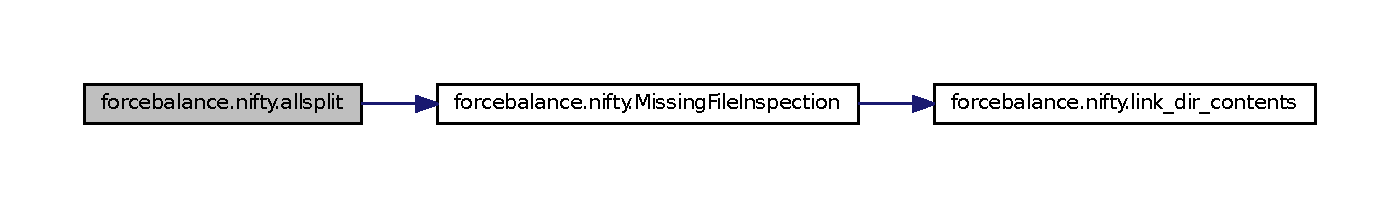
\includegraphics[width=350pt]{namespaceforcebalance_1_1nifty_ac9ab6c5543a2e3080061e0024850edf3_cgraph}
\end{center}
\end{figure}


\hypertarget{namespaceforcebalance_1_1nifty_afb3f205bce4984856e766af7e9fdaca8}{\index{forcebalance\-::nifty@{forcebalance\-::nifty}!col@{col}}
\index{col@{col}!forcebalance::nifty@{forcebalance\-::nifty}}
\paragraph[{col}]{\setlength{\rightskip}{0pt plus 5cm}def forcebalance.\-nifty.\-col (
\begin{DoxyParamCaption}
\item[{}]{vec}
\end{DoxyParamCaption}
)}}\label{namespaceforcebalance_1_1nifty_afb3f205bce4984856e766af7e9fdaca8}


Given any list, array, or matrix, return a 1-\/column matrix. 

Input\-: vec = The input vector that is to be made into a column

Output\-: A column matrix 

Definition at line 270 of file nifty.\-py.



Here is the call graph for this function\-:\nopagebreak
\begin{figure}[H]
\begin{center}
\leavevmode
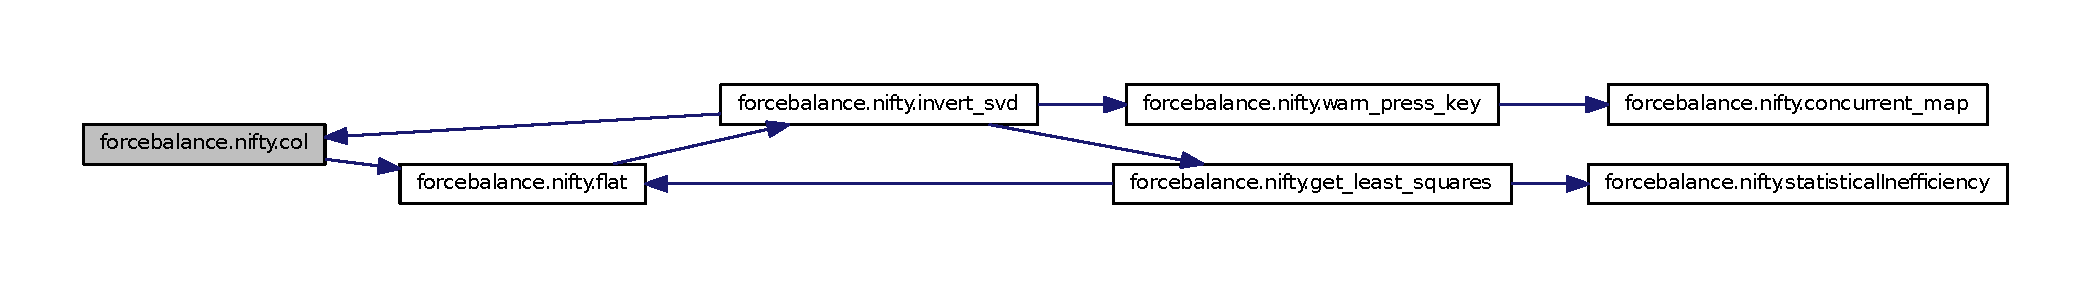
\includegraphics[width=350pt]{namespaceforcebalance_1_1nifty_afb3f205bce4984856e766af7e9fdaca8_cgraph}
\end{center}
\end{figure}


\hypertarget{namespaceforcebalance_1_1nifty_a9628ee448710667747d8aa5dc166532c}{\index{forcebalance\-::nifty@{forcebalance\-::nifty}!commadash@{commadash}}
\index{commadash@{commadash}!forcebalance::nifty@{forcebalance\-::nifty}}
\paragraph[{commadash}]{\setlength{\rightskip}{0pt plus 5cm}def forcebalance.\-nifty.\-commadash (
\begin{DoxyParamCaption}
\item[{}]{l}
\end{DoxyParamCaption}
)}}\label{namespaceforcebalance_1_1nifty_a9628ee448710667747d8aa5dc166532c}


Definition at line 81 of file nifty.\-py.



Here is the call graph for this function\-:\nopagebreak
\begin{figure}[H]
\begin{center}
\leavevmode
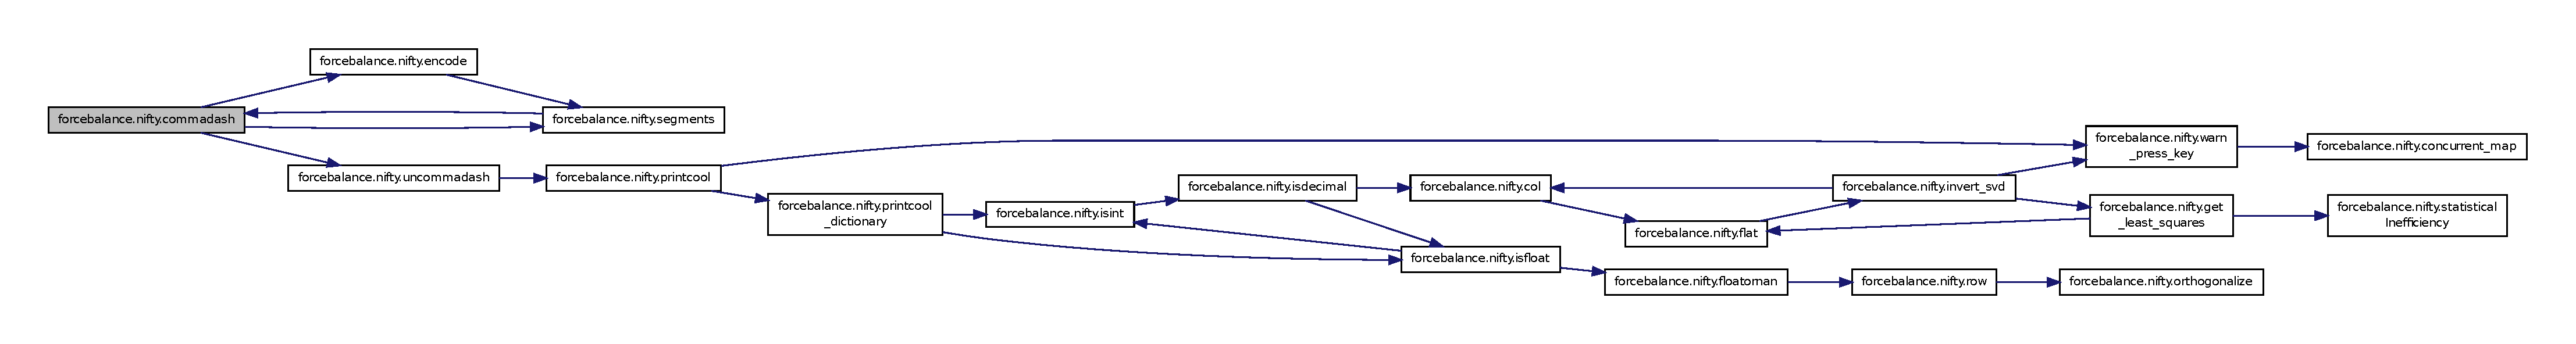
\includegraphics[width=350pt]{namespaceforcebalance_1_1nifty_a9628ee448710667747d8aa5dc166532c_cgraph}
\end{center}
\end{figure}


\hypertarget{namespaceforcebalance_1_1nifty_a2fc81730e7efa7d138dd86f733507bfc}{\index{forcebalance\-::nifty@{forcebalance\-::nifty}!concurrent\-\_\-map@{concurrent\-\_\-map}}
\index{concurrent\-\_\-map@{concurrent\-\_\-map}!forcebalance::nifty@{forcebalance\-::nifty}}
\paragraph[{concurrent\-\_\-map}]{\setlength{\rightskip}{0pt plus 5cm}def forcebalance.\-nifty.\-concurrent\-\_\-map (
\begin{DoxyParamCaption}
\item[{}]{func, }
\item[{}]{data}
\end{DoxyParamCaption}
)}}\label{namespaceforcebalance_1_1nifty_a2fc81730e7efa7d138dd86f733507bfc}


Similar to the bultin function map(). 

But spawn a thread for each argument and apply {\ttfamily func} concurrently.

Note\-: unlike map(), we cannot take an iterable argument. {\ttfamily data} should be an indexable sequence. 

Definition at line 911 of file nifty.\-py.

\hypertarget{namespaceforcebalance_1_1nifty_af5f0e1ba7689f1ab40383ba0480560a9}{\index{forcebalance\-::nifty@{forcebalance\-::nifty}!Copy\-File@{Copy\-File}}
\index{Copy\-File@{Copy\-File}!forcebalance::nifty@{forcebalance\-::nifty}}
\paragraph[{Copy\-File}]{\setlength{\rightskip}{0pt plus 5cm}def forcebalance.\-nifty.\-Copy\-File (
\begin{DoxyParamCaption}
\item[{}]{src, }
\item[{}]{dest}
\end{DoxyParamCaption}
)}}\label{namespaceforcebalance_1_1nifty_af5f0e1ba7689f1ab40383ba0480560a9}


Definition at line 754 of file nifty.\-py.



Here is the call graph for this function\-:\nopagebreak
\begin{figure}[H]
\begin{center}
\leavevmode
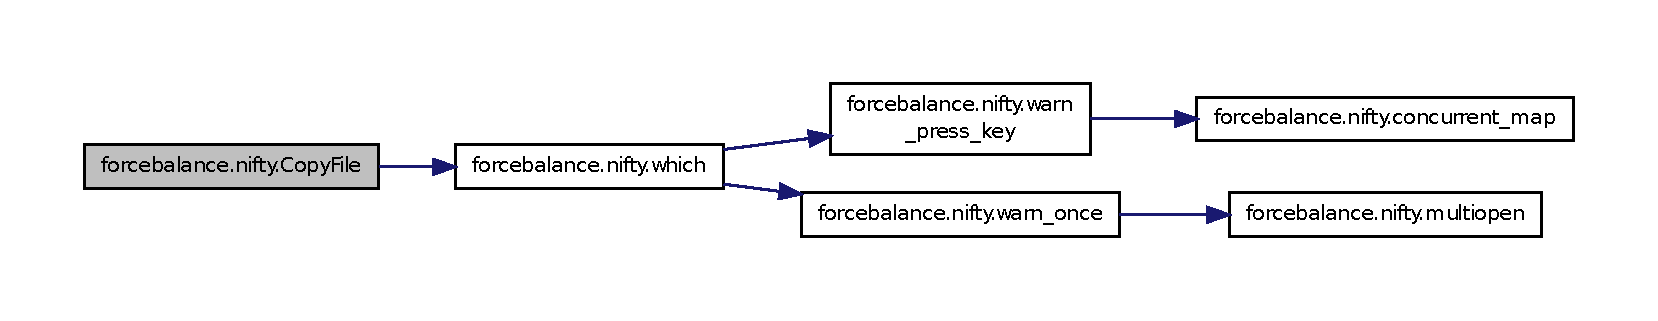
\includegraphics[width=350pt]{namespaceforcebalance_1_1nifty_af5f0e1ba7689f1ab40383ba0480560a9_cgraph}
\end{center}
\end{figure}


\hypertarget{namespaceforcebalance_1_1nifty_ab5f3072ad95e9c75659cb1adac341051}{\index{forcebalance\-::nifty@{forcebalance\-::nifty}!create\-Work\-Queue@{create\-Work\-Queue}}
\index{create\-Work\-Queue@{create\-Work\-Queue}!forcebalance::nifty@{forcebalance\-::nifty}}
\paragraph[{create\-Work\-Queue}]{\setlength{\rightskip}{0pt plus 5cm}def forcebalance.\-nifty.\-create\-Work\-Queue (
\begin{DoxyParamCaption}
\item[{}]{wq\-\_\-port, }
\item[{}]{debug = {\ttfamily True}}
\end{DoxyParamCaption}
)}}\label{namespaceforcebalance_1_1nifty_ab5f3072ad95e9c75659cb1adac341051}


Definition at line 572 of file nifty.\-py.



Here is the call graph for this function\-:\nopagebreak
\begin{figure}[H]
\begin{center}
\leavevmode
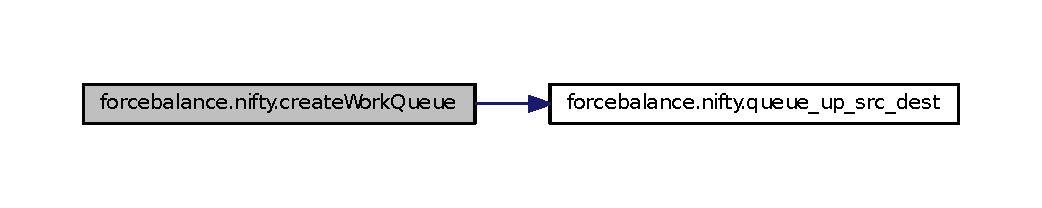
\includegraphics[width=350pt]{namespaceforcebalance_1_1nifty_ab5f3072ad95e9c75659cb1adac341051_cgraph}
\end{center}
\end{figure}


\hypertarget{namespaceforcebalance_1_1nifty_a3b437964dc22735bf8a7dcbaf99e413d}{\index{forcebalance\-::nifty@{forcebalance\-::nifty}!encode@{encode}}
\index{encode@{encode}!forcebalance::nifty@{forcebalance\-::nifty}}
\paragraph[{encode}]{\setlength{\rightskip}{0pt plus 5cm}def forcebalance.\-nifty.\-encode (
\begin{DoxyParamCaption}
\item[{}]{l}
\end{DoxyParamCaption}
)}}\label{namespaceforcebalance_1_1nifty_a3b437964dc22735bf8a7dcbaf99e413d}


Definition at line 72 of file nifty.\-py.



Here is the call graph for this function\-:\nopagebreak
\begin{figure}[H]
\begin{center}
\leavevmode
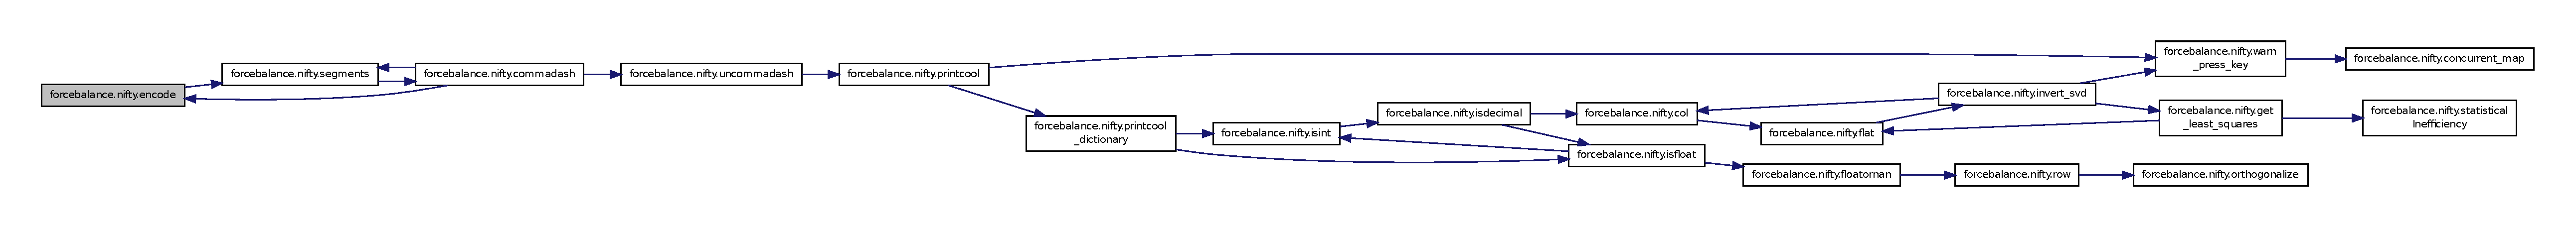
\includegraphics[width=350pt]{namespaceforcebalance_1_1nifty_a3b437964dc22735bf8a7dcbaf99e413d_cgraph}
\end{center}
\end{figure}


\hypertarget{namespaceforcebalance_1_1nifty_a52114ceee9d55f94d9aecb3e176de294}{\index{forcebalance\-::nifty@{forcebalance\-::nifty}!flat@{flat}}
\index{flat@{flat}!forcebalance::nifty@{forcebalance\-::nifty}}
\paragraph[{flat}]{\setlength{\rightskip}{0pt plus 5cm}def forcebalance.\-nifty.\-flat (
\begin{DoxyParamCaption}
\item[{}]{vec}
\end{DoxyParamCaption}
)}}\label{namespaceforcebalance_1_1nifty_a52114ceee9d55f94d9aecb3e176de294}


Given any list, array, or matrix, return a single-\/index array. 


\begin{DoxyParams}[1]{Parameters}
\mbox{\tt in}  & {\em vec} & The data to be flattened \\
\hline
\end{DoxyParams}
\begin{DoxyReturn}{Returns}
answer The flattened data 
\end{DoxyReturn}


Definition at line 289 of file nifty.\-py.



Here is the call graph for this function\-:\nopagebreak
\begin{figure}[H]
\begin{center}
\leavevmode
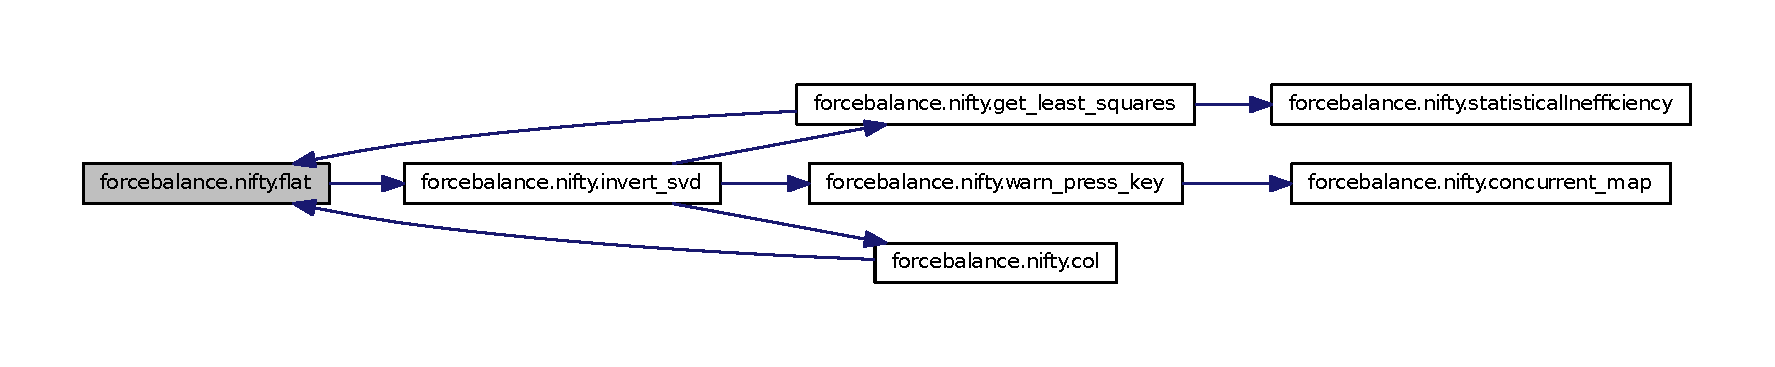
\includegraphics[width=350pt]{namespaceforcebalance_1_1nifty_a52114ceee9d55f94d9aecb3e176de294_cgraph}
\end{center}
\end{figure}


\hypertarget{namespaceforcebalance_1_1nifty_a8d63c8ae9a67c66673a6cf81357f827d}{\index{forcebalance\-::nifty@{forcebalance\-::nifty}!floatornan@{floatornan}}
\index{floatornan@{floatornan}!forcebalance::nifty@{forcebalance\-::nifty}}
\paragraph[{floatornan}]{\setlength{\rightskip}{0pt plus 5cm}def forcebalance.\-nifty.\-floatornan (
\begin{DoxyParamCaption}
\item[{}]{word}
\end{DoxyParamCaption}
)}}\label{namespaceforcebalance_1_1nifty_a8d63c8ae9a67c66673a6cf81357f827d}


Returns a big number if we encounter Na\-N. 


\begin{DoxyParams}[1]{Parameters}
\mbox{\tt in}  & {\em word} & The string to be converted \\
\hline
\end{DoxyParams}
\begin{DoxyReturn}{Returns}
answer The string converted to a float; if not a float, return 1e10 
\end{DoxyReturn}
\begin{DoxyRefDesc}{Todo}
\item[\hyperlink{todo__todo000013}{Todo}]I could use suggestions for making this better. \end{DoxyRefDesc}


Definition at line 252 of file nifty.\-py.



Here is the call graph for this function\-:\nopagebreak
\begin{figure}[H]
\begin{center}
\leavevmode
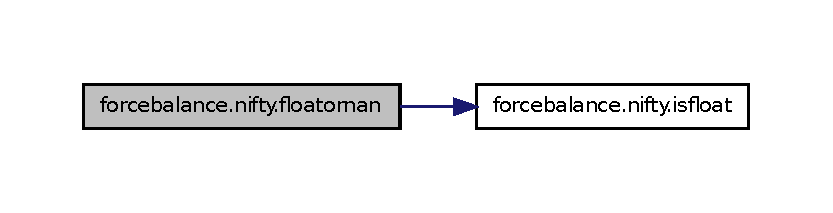
\includegraphics[width=350pt]{namespaceforcebalance_1_1nifty_a8d63c8ae9a67c66673a6cf81357f827d_cgraph}
\end{center}
\end{figure}


\hypertarget{namespaceforcebalance_1_1nifty_aa9fb9c7c65231eca50a7afc04f489b64}{\index{forcebalance\-::nifty@{forcebalance\-::nifty}!get\-\_\-least\-\_\-squares@{get\-\_\-least\-\_\-squares}}
\index{get\-\_\-least\-\_\-squares@{get\-\_\-least\-\_\-squares}!forcebalance::nifty@{forcebalance\-::nifty}}
\paragraph[{get\-\_\-least\-\_\-squares}]{\setlength{\rightskip}{0pt plus 5cm}def forcebalance.\-nifty.\-get\-\_\-least\-\_\-squares (
\begin{DoxyParamCaption}
\item[{}]{x, }
\item[{}]{y, }
\item[{}]{w = {\ttfamily None}, }
\item[{}]{thresh = {\ttfamily 1e-\/12}}
\end{DoxyParamCaption}
)}}\label{namespaceforcebalance_1_1nifty_aa9fb9c7c65231eca50a7afc04f489b64}

\begin{DoxyCode}
1  \_\_                  \_\_
2 |                      |
3 | 1 (x0) (x0)^2 (x0)^3 |
4 | 1 (x1) (x1)^2 (x1)^3 |
5 | 1 (x2) (x2)^2 (x2)^3 |
6 | 1 (x3) (x3)^2 (x3)^3 |
7 | 1 (x4) (x4)^2 (x4)^3 |
8 |\_\_                  \_\_|
\end{DoxyCode}



\begin{DoxyParams}[1]{Parameters}
\mbox{\tt in}  & {\em X} & (2-\/\-D array) An array of X-\/values (see above) \\
\hline
\mbox{\tt in}  & {\em Y} & (array) An array of Y-\/values (only used in getting the least squares coefficients) \\
\hline
\mbox{\tt in}  & {\em w} & (array) An array of weights, hopefully normalized to one. \\
\hline
\mbox{\tt out}  & {\em Beta} & The least-\/squares coefficients \\
\hline
\mbox{\tt out}  & {\em Hat} & The hat matrix that takes linear combinations of data y-\/values to give fitted y-\/values (weights) \\
\hline
\mbox{\tt out}  & {\em yfit} & The fitted y-\/values \\
\hline
\mbox{\tt out}  & {\em M\-P\-P\-I} & The Moore-\/\-Penrose pseudoinverse (multiply by Y to get least-\/squares coefficients, multiply by d\-Y/dk to get derivatives of least-\/squares coefficients) \\
\hline
\end{DoxyParams}


Definition at line 357 of file nifty.\-py.



Here is the call graph for this function\-:\nopagebreak
\begin{figure}[H]
\begin{center}
\leavevmode
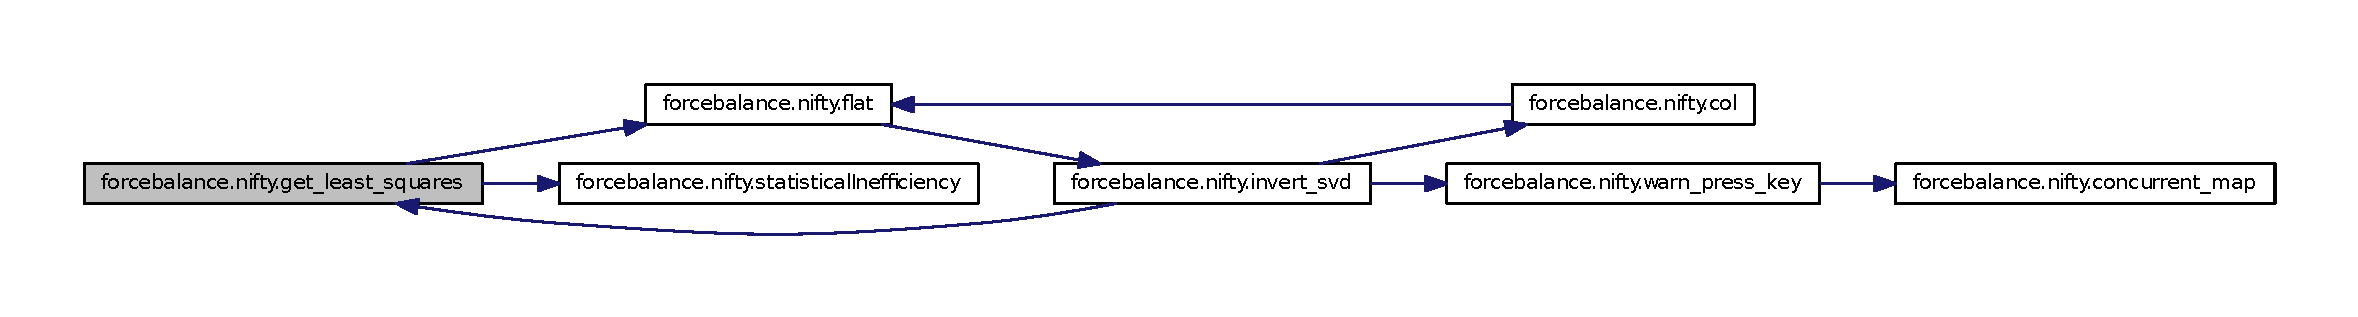
\includegraphics[width=350pt]{namespaceforcebalance_1_1nifty_aa9fb9c7c65231eca50a7afc04f489b64_cgraph}
\end{center}
\end{figure}


\hypertarget{namespaceforcebalance_1_1nifty_ac37d4fe58ef70ed546ebfc45d12f7a5d}{\index{forcebalance\-::nifty@{forcebalance\-::nifty}!get\-Work\-Queue@{get\-Work\-Queue}}
\index{get\-Work\-Queue@{get\-Work\-Queue}!forcebalance::nifty@{forcebalance\-::nifty}}
\paragraph[{get\-Work\-Queue}]{\setlength{\rightskip}{0pt plus 5cm}def forcebalance.\-nifty.\-get\-Work\-Queue (
\begin{DoxyParamCaption}
{}
\end{DoxyParamCaption}
)}}\label{namespaceforcebalance_1_1nifty_ac37d4fe58ef70ed546ebfc45d12f7a5d}


Definition at line 566 of file nifty.\-py.

\hypertarget{namespaceforcebalance_1_1nifty_abe1e72c32252d62a6551b47290c7584f}{\index{forcebalance\-::nifty@{forcebalance\-::nifty}!get\-W\-Q\-Ids@{get\-W\-Q\-Ids}}
\index{get\-W\-Q\-Ids@{get\-W\-Q\-Ids}!forcebalance::nifty@{forcebalance\-::nifty}}
\paragraph[{get\-W\-Q\-Ids}]{\setlength{\rightskip}{0pt plus 5cm}def forcebalance.\-nifty.\-get\-W\-Q\-Ids (
\begin{DoxyParamCaption}
{}
\end{DoxyParamCaption}
)}}\label{namespaceforcebalance_1_1nifty_abe1e72c32252d62a6551b47290c7584f}


Definition at line 569 of file nifty.\-py.

\hypertarget{namespaceforcebalance_1_1nifty_ad432b88307e1178b0690c0d350b1af36}{\index{forcebalance\-::nifty@{forcebalance\-::nifty}!Go\-Into@{Go\-Into}}
\index{Go\-Into@{Go\-Into}!forcebalance::nifty@{forcebalance\-::nifty}}
\paragraph[{Go\-Into}]{\setlength{\rightskip}{0pt plus 5cm}def forcebalance.\-nifty.\-Go\-Into (
\begin{DoxyParamCaption}
\item[{}]{Dir}
\end{DoxyParamCaption}
)}}\label{namespaceforcebalance_1_1nifty_ad432b88307e1178b0690c0d350b1af36}


Definition at line 698 of file nifty.\-py.

\hypertarget{namespaceforcebalance_1_1nifty_a4c82187e92dfeb8a159f4aa44b501c40}{\index{forcebalance\-::nifty@{forcebalance\-::nifty}!invert\-\_\-svd@{invert\-\_\-svd}}
\index{invert\-\_\-svd@{invert\-\_\-svd}!forcebalance::nifty@{forcebalance\-::nifty}}
\paragraph[{invert\-\_\-svd}]{\setlength{\rightskip}{0pt plus 5cm}def forcebalance.\-nifty.\-invert\-\_\-svd (
\begin{DoxyParamCaption}
\item[{}]{X, }
\item[{}]{thresh = {\ttfamily 1e-\/12}}
\end{DoxyParamCaption}
)}}\label{namespaceforcebalance_1_1nifty_a4c82187e92dfeb8a159f4aa44b501c40}


Invert a matrix using singular value decomposition. 


\begin{DoxyParams}[1]{Parameters}
\mbox{\tt in}  & {\em X} & The matrix to be inverted \\
\hline
\mbox{\tt in}  & {\em thresh} & The S\-V\-D threshold; eigenvalues below this are not inverted but set to zero \\
\hline
\end{DoxyParams}
\begin{DoxyReturn}{Returns}
Xt The inverted matrix 
\end{DoxyReturn}


Definition at line 316 of file nifty.\-py.



Here is the call graph for this function\-:\nopagebreak
\begin{figure}[H]
\begin{center}
\leavevmode
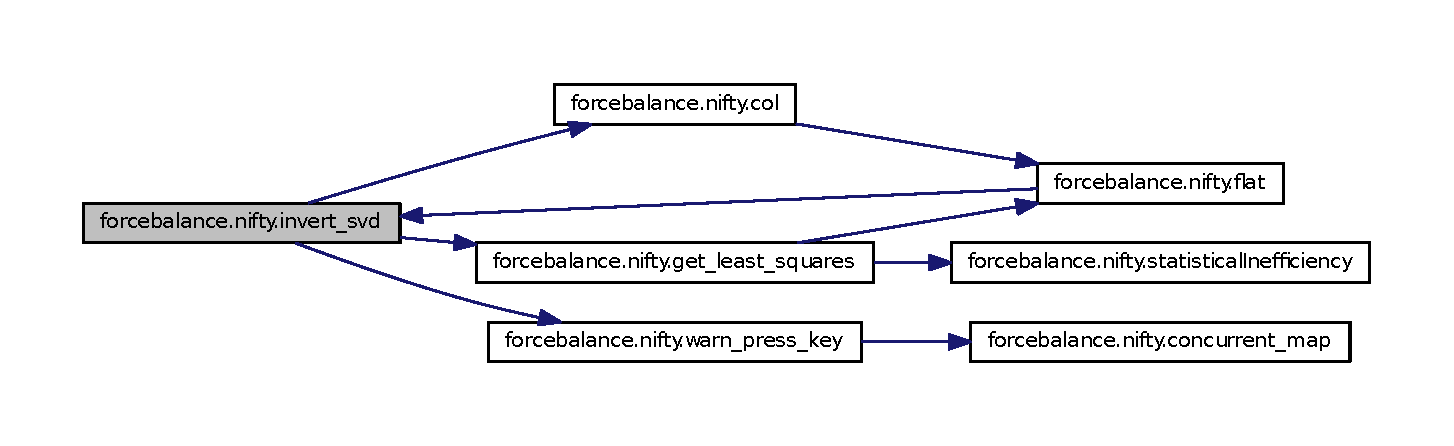
\includegraphics[width=350pt]{namespaceforcebalance_1_1nifty_a4c82187e92dfeb8a159f4aa44b501c40_cgraph}
\end{center}
\end{figure}


\hypertarget{namespaceforcebalance_1_1nifty_a09263927eaec9deff283fbf1a820242f}{\index{forcebalance\-::nifty@{forcebalance\-::nifty}!isdecimal@{isdecimal}}
\index{isdecimal@{isdecimal}!forcebalance::nifty@{forcebalance\-::nifty}}
\paragraph[{isdecimal}]{\setlength{\rightskip}{0pt plus 5cm}def forcebalance.\-nifty.\-isdecimal (
\begin{DoxyParamCaption}
\item[{}]{word}
\end{DoxyParamCaption}
)}}\label{namespaceforcebalance_1_1nifty_a09263927eaec9deff283fbf1a820242f}


Matches things with a decimal only; see isint and isfloat. 


\begin{DoxyParams}[1]{Parameters}
\mbox{\tt in}  & {\em word} & String (for instance, '123', '153.\-0', '2.', '-\/354') \\
\hline
\end{DoxyParams}
\begin{DoxyReturn}{Returns}
answer Boolean which specifies whether the string is a number with a decimal point 
\end{DoxyReturn}


Definition at line 242 of file nifty.\-py.



Here is the call graph for this function\-:\nopagebreak
\begin{figure}[H]
\begin{center}
\leavevmode
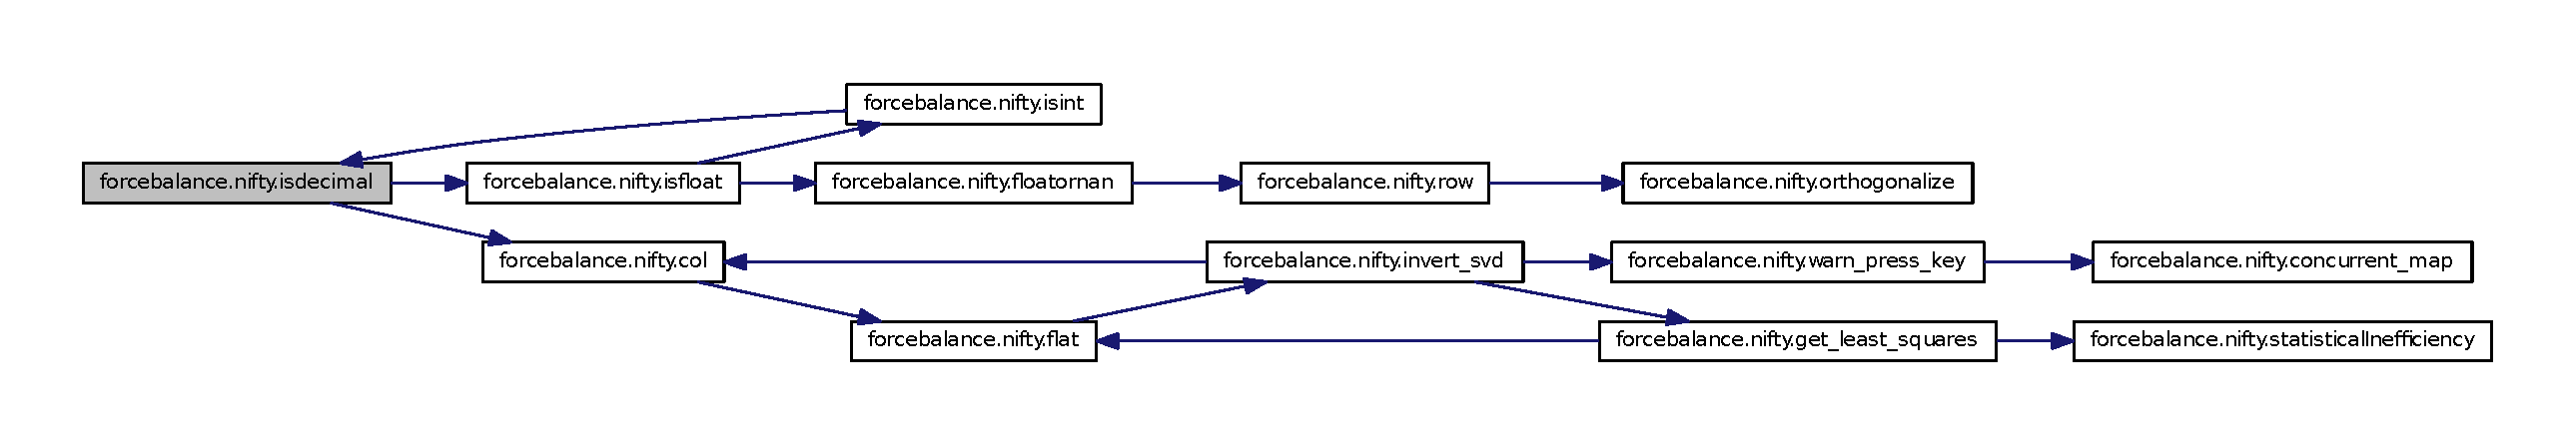
\includegraphics[width=350pt]{namespaceforcebalance_1_1nifty_a09263927eaec9deff283fbf1a820242f_cgraph}
\end{center}
\end{figure}


\hypertarget{namespaceforcebalance_1_1nifty_a8e3ef0108b9d37b82ba0dced7c6037ae}{\index{forcebalance\-::nifty@{forcebalance\-::nifty}!isfloat@{isfloat}}
\index{isfloat@{isfloat}!forcebalance::nifty@{forcebalance\-::nifty}}
\paragraph[{isfloat}]{\setlength{\rightskip}{0pt plus 5cm}def forcebalance.\-nifty.\-isfloat (
\begin{DoxyParamCaption}
\item[{}]{word}
\end{DoxyParamCaption}
)}}\label{namespaceforcebalance_1_1nifty_a8e3ef0108b9d37b82ba0dced7c6037ae}


Matches A\-N\-Y number; it can be a decimal, scientific notation, what have you C\-A\-U\-T\-I\-O\-N -\/ this will also match an integer. 


\begin{DoxyParams}[1]{Parameters}
\mbox{\tt in}  & {\em word} & String (for instance, '123', '153.\-0', '2.', '-\/354') \\
\hline
\end{DoxyParams}
\begin{DoxyReturn}{Returns}
answer Boolean which specifies whether the string is any number 
\end{DoxyReturn}


Definition at line 232 of file nifty.\-py.



Here is the call graph for this function\-:\nopagebreak
\begin{figure}[H]
\begin{center}
\leavevmode
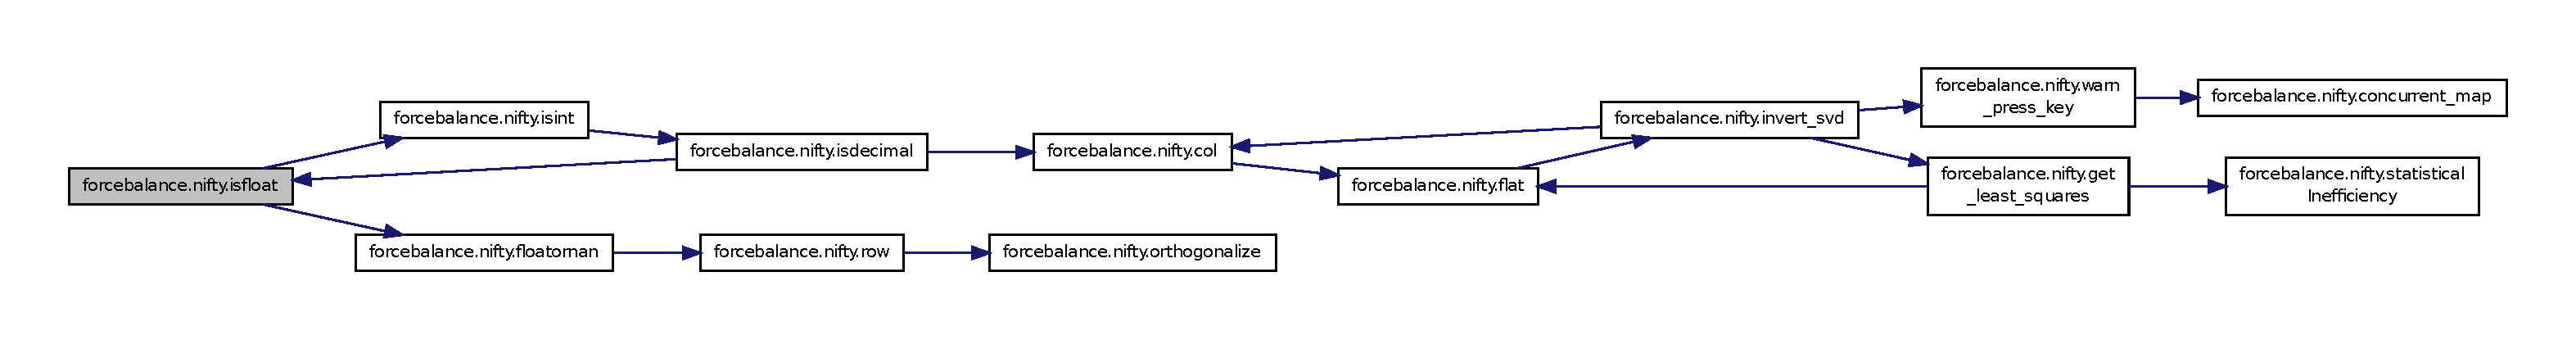
\includegraphics[width=350pt]{namespaceforcebalance_1_1nifty_a8e3ef0108b9d37b82ba0dced7c6037ae_cgraph}
\end{center}
\end{figure}


\hypertarget{namespaceforcebalance_1_1nifty_a3f1c7a1af9d35d5d1693074bc6f5497c}{\index{forcebalance\-::nifty@{forcebalance\-::nifty}!isint@{isint}}
\index{isint@{isint}!forcebalance::nifty@{forcebalance\-::nifty}}
\paragraph[{isint}]{\setlength{\rightskip}{0pt plus 5cm}def forcebalance.\-nifty.\-isint (
\begin{DoxyParamCaption}
\item[{}]{word}
\end{DoxyParamCaption}
)}}\label{namespaceforcebalance_1_1nifty_a3f1c7a1af9d35d5d1693074bc6f5497c}


O\-N\-L\-Y matches integers! If you have a decimal point? None shall pass! 


\begin{DoxyParams}[1]{Parameters}
\mbox{\tt in}  & {\em word} & String (for instance, '123', '153.\-0', '2.', '-\/354') \\
\hline
\end{DoxyParams}
\begin{DoxyReturn}{Returns}
answer Boolean which specifies whether the string is an integer (only +/-\/ sign followed by digits) 
\end{DoxyReturn}


Definition at line 221 of file nifty.\-py.



Here is the call graph for this function\-:\nopagebreak
\begin{figure}[H]
\begin{center}
\leavevmode
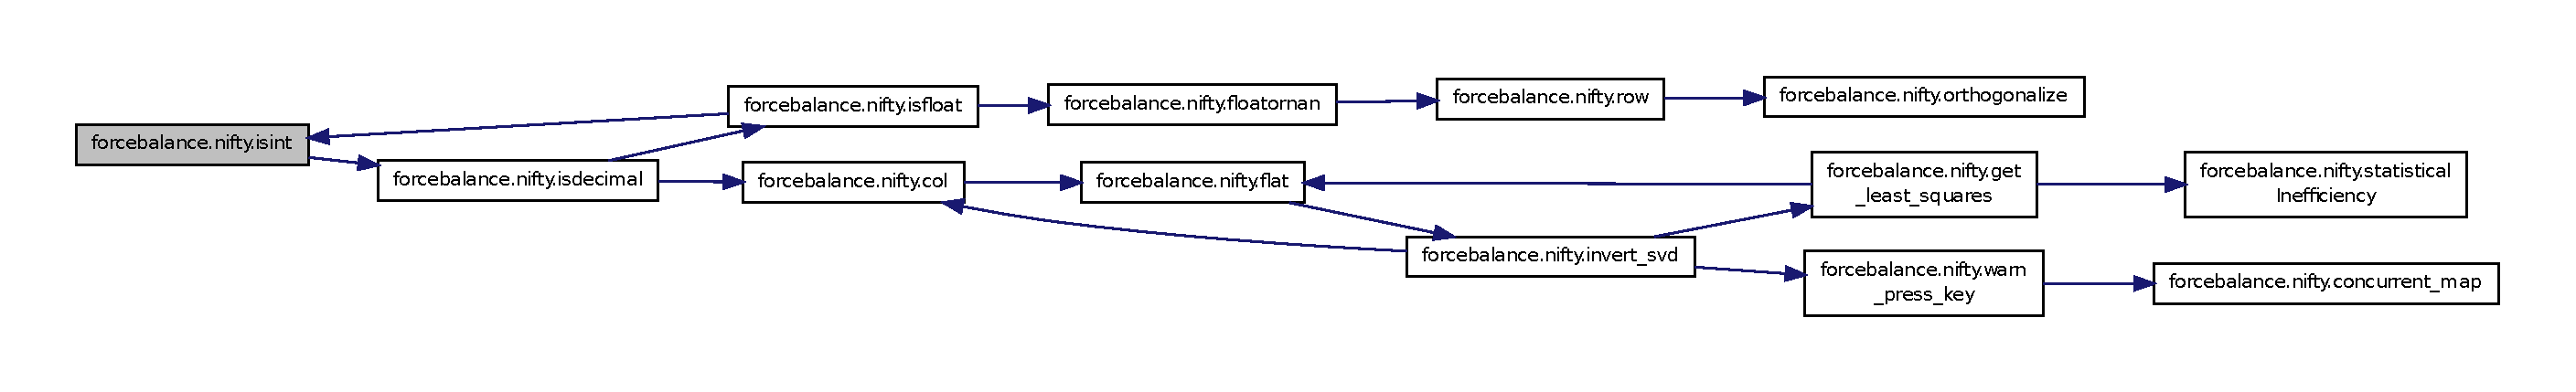
\includegraphics[width=350pt]{namespaceforcebalance_1_1nifty_a3f1c7a1af9d35d5d1693074bc6f5497c_cgraph}
\end{center}
\end{figure}


\hypertarget{namespaceforcebalance_1_1nifty_ab04e8690d099db2379dc860e0d040120}{\index{forcebalance\-::nifty@{forcebalance\-::nifty}!Leave@{Leave}}
\index{Leave@{Leave}!forcebalance::nifty@{forcebalance\-::nifty}}
\paragraph[{Leave}]{\setlength{\rightskip}{0pt plus 5cm}def forcebalance.\-nifty.\-Leave (
\begin{DoxyParamCaption}
\item[{}]{Dir}
\end{DoxyParamCaption}
)}}\label{namespaceforcebalance_1_1nifty_ab04e8690d099db2379dc860e0d040120}


Definition at line 712 of file nifty.\-py.

\hypertarget{namespaceforcebalance_1_1nifty_a0cf4e58f90acf20e3d6224be2354082c}{\index{forcebalance\-::nifty@{forcebalance\-::nifty}!link\-\_\-dir\-\_\-contents@{link\-\_\-dir\-\_\-contents}}
\index{link\-\_\-dir\-\_\-contents@{link\-\_\-dir\-\_\-contents}!forcebalance::nifty@{forcebalance\-::nifty}}
\paragraph[{link\-\_\-dir\-\_\-contents}]{\setlength{\rightskip}{0pt plus 5cm}def forcebalance.\-nifty.\-link\-\_\-dir\-\_\-contents (
\begin{DoxyParamCaption}
\item[{}]{abssrcdir, }
\item[{}]{absdestdir}
\end{DoxyParamCaption}
)}}\label{namespaceforcebalance_1_1nifty_a0cf4e58f90acf20e3d6224be2354082c}


Definition at line 764 of file nifty.\-py.

\hypertarget{namespaceforcebalance_1_1nifty_ab182a9da2a2f42cf45942fbee6acf9b1}{\index{forcebalance\-::nifty@{forcebalance\-::nifty}!Link\-File@{Link\-File}}
\index{Link\-File@{Link\-File}!forcebalance::nifty@{forcebalance\-::nifty}}
\paragraph[{Link\-File}]{\setlength{\rightskip}{0pt plus 5cm}def forcebalance.\-nifty.\-Link\-File (
\begin{DoxyParamCaption}
\item[{}]{src, }
\item[{}]{dest}
\end{DoxyParamCaption}
)}}\label{namespaceforcebalance_1_1nifty_ab182a9da2a2f42cf45942fbee6acf9b1}


Definition at line 743 of file nifty.\-py.



Here is the call graph for this function\-:\nopagebreak
\begin{figure}[H]
\begin{center}
\leavevmode
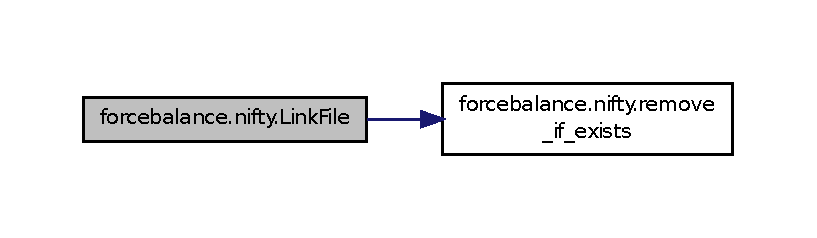
\includegraphics[width=350pt]{namespaceforcebalance_1_1nifty_ab182a9da2a2f42cf45942fbee6acf9b1_cgraph}
\end{center}
\end{figure}


\hypertarget{namespaceforcebalance_1_1nifty_a2ff762a2f2d2b6bb1c7dd067bd1a1e88}{\index{forcebalance\-::nifty@{forcebalance\-::nifty}!lp\-\_\-dump@{lp\-\_\-dump}}
\index{lp\-\_\-dump@{lp\-\_\-dump}!forcebalance::nifty@{forcebalance\-::nifty}}
\paragraph[{lp\-\_\-dump}]{\setlength{\rightskip}{0pt plus 5cm}def forcebalance.\-nifty.\-lp\-\_\-dump (
\begin{DoxyParamCaption}
\item[{}]{obj, }
\item[{}]{file, }
\item[{}]{protocol = {\ttfamily None}}
\end{DoxyParamCaption}
)}}\label{namespaceforcebalance_1_1nifty_a2ff762a2f2d2b6bb1c7dd067bd1a1e88}


Use this instead of pickle.\-dump for pickling anything that contains \-\_\-\-Element\-Tree types. 



Definition at line 549 of file nifty.\-py.



Here is the call graph for this function\-:\nopagebreak
\begin{figure}[H]
\begin{center}
\leavevmode
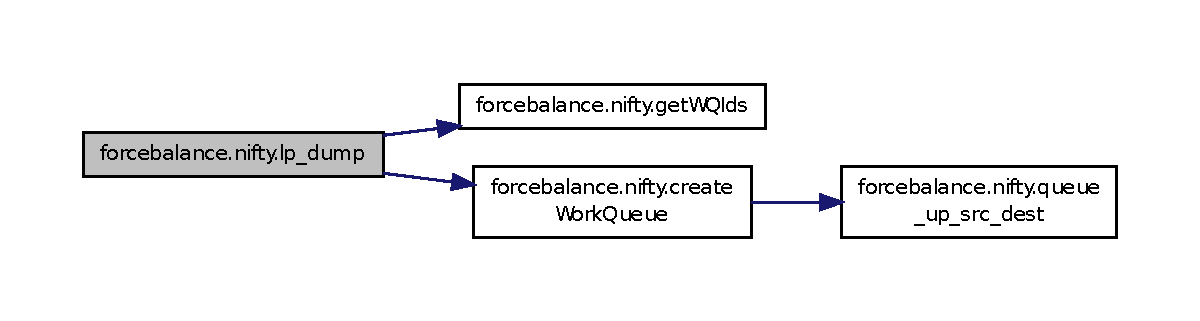
\includegraphics[width=350pt]{namespaceforcebalance_1_1nifty_a2ff762a2f2d2b6bb1c7dd067bd1a1e88_cgraph}
\end{center}
\end{figure}


\hypertarget{namespaceforcebalance_1_1nifty_a577abfd36638c5f4dfdade136abaef12}{\index{forcebalance\-::nifty@{forcebalance\-::nifty}!lp\-\_\-load@{lp\-\_\-load}}
\index{lp\-\_\-load@{lp\-\_\-load}!forcebalance::nifty@{forcebalance\-::nifty}}
\paragraph[{lp\-\_\-load}]{\setlength{\rightskip}{0pt plus 5cm}def forcebalance.\-nifty.\-lp\-\_\-load (
\begin{DoxyParamCaption}
\item[{}]{file}
\end{DoxyParamCaption}
)}}\label{namespaceforcebalance_1_1nifty_a577abfd36638c5f4dfdade136abaef12}


Use this instead of pickle.\-load for unpickling anything that contains \-\_\-\-Element\-Tree types. 



Definition at line 554 of file nifty.\-py.



Here is the call graph for this function\-:\nopagebreak
\begin{figure}[H]
\begin{center}
\leavevmode
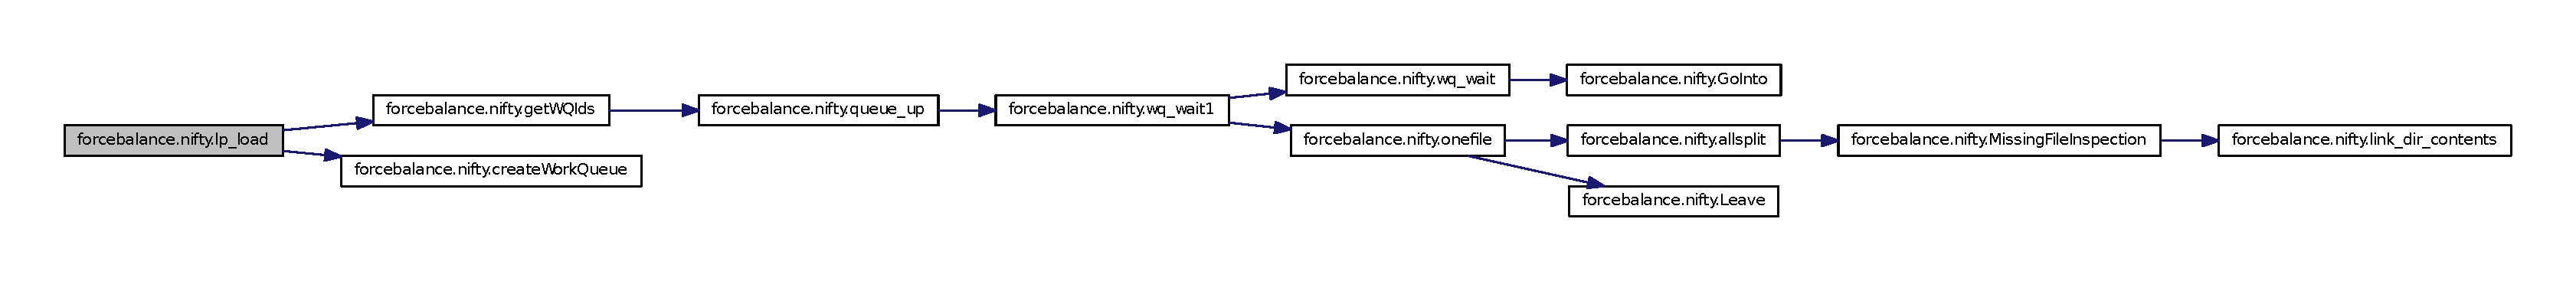
\includegraphics[width=350pt]{namespaceforcebalance_1_1nifty_a577abfd36638c5f4dfdade136abaef12_cgraph}
\end{center}
\end{figure}


\hypertarget{namespaceforcebalance_1_1nifty_ae87c7def5f8edf2ec30737bdb1d2636f}{\index{forcebalance\-::nifty@{forcebalance\-::nifty}!Missing\-File\-Inspection@{Missing\-File\-Inspection}}
\index{Missing\-File\-Inspection@{Missing\-File\-Inspection}!forcebalance::nifty@{forcebalance\-::nifty}}
\paragraph[{Missing\-File\-Inspection}]{\setlength{\rightskip}{0pt plus 5cm}def forcebalance.\-nifty.\-Missing\-File\-Inspection (
\begin{DoxyParamCaption}
\item[{}]{fnm}
\end{DoxyParamCaption}
)}}\label{namespaceforcebalance_1_1nifty_ae87c7def5f8edf2ec30737bdb1d2636f}


Definition at line 733 of file nifty.\-py.



Here is the call graph for this function\-:\nopagebreak
\begin{figure}[H]
\begin{center}
\leavevmode
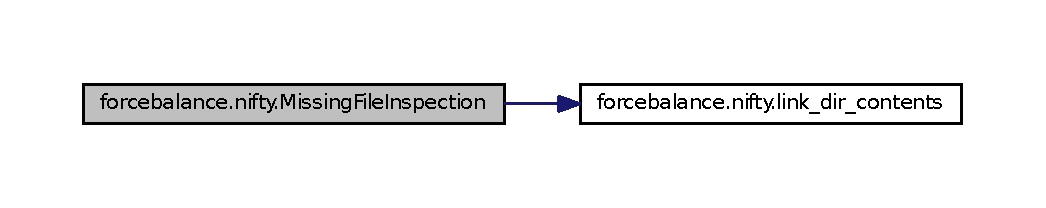
\includegraphics[width=350pt]{namespaceforcebalance_1_1nifty_ae87c7def5f8edf2ec30737bdb1d2636f_cgraph}
\end{center}
\end{figure}


\hypertarget{namespaceforcebalance_1_1nifty_a64b7c6ca7afa1c11681f5c2897c55cc3}{\index{forcebalance\-::nifty@{forcebalance\-::nifty}!multiopen@{multiopen}}
\index{multiopen@{multiopen}!forcebalance::nifty@{forcebalance\-::nifty}}
\paragraph[{multiopen}]{\setlength{\rightskip}{0pt plus 5cm}def forcebalance.\-nifty.\-multiopen (
\begin{DoxyParamCaption}
\item[{}]{arg}
\end{DoxyParamCaption}
)}}\label{namespaceforcebalance_1_1nifty_a64b7c6ca7afa1c11681f5c2897c55cc3}


This function be given any of several variable types (single file name, file object, or list of lines, or a list of the above) and give a list of files\-: 

\mbox{[}file1, file2, file3 ... \mbox{]}

each of which can then be iterated over\-:

\mbox{[}\mbox{[}file1\-\_\-line1, file1\-\_\-line2 ... \mbox{]}, \mbox{[}file2\-\_\-line1, file2\-\_\-line2 ... \mbox{]}\mbox{]} 

Definition at line 941 of file nifty.\-py.

\hypertarget{namespaceforcebalance_1_1nifty_a7676236002c6a65ea7d2e69a09923889}{\index{forcebalance\-::nifty@{forcebalance\-::nifty}!orthogonalize@{orthogonalize}}
\index{orthogonalize@{orthogonalize}!forcebalance::nifty@{forcebalance\-::nifty}}
\paragraph[{orthogonalize}]{\setlength{\rightskip}{0pt plus 5cm}def forcebalance.\-nifty.\-orthogonalize (
\begin{DoxyParamCaption}
\item[{}]{vec1, }
\item[{}]{vec2}
\end{DoxyParamCaption}
)}}\label{namespaceforcebalance_1_1nifty_a7676236002c6a65ea7d2e69a09923889}


Given two vectors vec1 and vec2, project out the component of vec1 that is along the vec2-\/direction. 


\begin{DoxyParams}[1]{Parameters}
\mbox{\tt in}  & {\em vec1} & The projectee (i.\-e. output is some modified version of vec1) \\
\hline
\mbox{\tt in}  & {\em vec2} & The projector (component subtracted out from vec1 is parallel to this) \\
\hline
\end{DoxyParams}
\begin{DoxyReturn}{Returns}
answer A copy of vec1 but with the vec2-\/component projected out. 
\end{DoxyReturn}


Definition at line 303 of file nifty.\-py.

\hypertarget{namespaceforcebalance_1_1nifty_af61d76c8eb78c8ee52a43e239ff26cb4}{\index{forcebalance\-::nifty@{forcebalance\-::nifty}!pmat2d@{pmat2d}}
\index{pmat2d@{pmat2d}!forcebalance::nifty@{forcebalance\-::nifty}}
\paragraph[{pmat2d}]{\setlength{\rightskip}{0pt plus 5cm}def forcebalance.\-nifty.\-pmat2d (
\begin{DoxyParamCaption}
\item[{}]{mat2d, }
\item[{}]{precision = {\ttfamily 1}, }
\item[{}]{loglevel = {\ttfamily forcebalance.output.INFO}}
\end{DoxyParamCaption}
)}}\label{namespaceforcebalance_1_1nifty_af61d76c8eb78c8ee52a43e239ff26cb4}


Printout of a 2-\/\-D matrix. 


\begin{DoxyParams}[1]{Parameters}
\mbox{\tt in}  & {\em mat2d} & a 2-\/\-D matrix \\
\hline
\end{DoxyParams}


Definition at line 65 of file nifty.\-py.



Here is the call graph for this function\-:\nopagebreak
\begin{figure}[H]
\begin{center}
\leavevmode
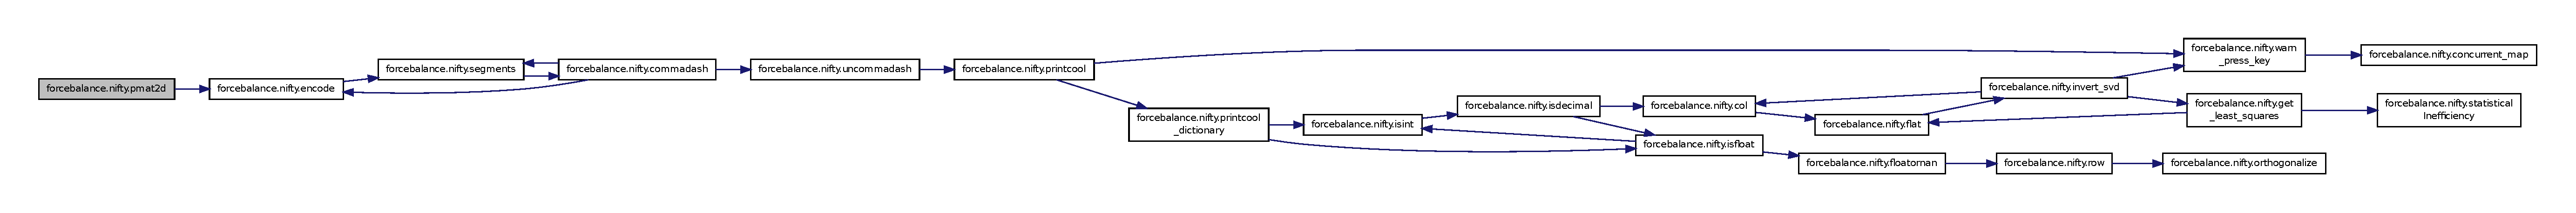
\includegraphics[width=350pt]{namespaceforcebalance_1_1nifty_af61d76c8eb78c8ee52a43e239ff26cb4_cgraph}
\end{center}
\end{figure}


\hypertarget{namespaceforcebalance_1_1nifty_a11babd62dc7bca389162c6318f9672ca}{\index{forcebalance\-::nifty@{forcebalance\-::nifty}!printcool@{printcool}}
\index{printcool@{printcool}!forcebalance::nifty@{forcebalance\-::nifty}}
\paragraph[{printcool}]{\setlength{\rightskip}{0pt plus 5cm}def forcebalance.\-nifty.\-printcool (
\begin{DoxyParamCaption}
\item[{}]{text, }
\item[{}]{sym = {\ttfamily \char`\"{}\#\char`\"{}}, }
\item[{}]{bold = {\ttfamily False}, }
\item[{}]{color = {\ttfamily 2}, }
\item[{}]{ansi = {\ttfamily None}, }
\item[{}]{bottom = {\ttfamily '-\/'}, }
\item[{}]{minwidth = {\ttfamily 50}, }
\item[{}]{center = {\ttfamily True}}
\end{DoxyParamCaption}
)}}\label{namespaceforcebalance_1_1nifty_a11babd62dc7bca389162c6318f9672ca}


Cool-\/looking printout for slick formatting of output. 


\begin{DoxyParams}[1]{Parameters}
\mbox{\tt in}  & {\em text} & The string that the printout is based upon. This function will print out the string, A\-N\-S\-I-\/colored and enclosed in the symbol for example\-:\par
 {\ttfamily  \#\#\#\#\#\#\#\#\#\#\#\#\#\#\#\#\# }\par
 {\ttfamily  \#\#\# I am cool \#\#\# }\par
 {\ttfamily  \#\#\#\#\#\#\#\#\#\#\#\#\#\#\#\#\# } \\
\hline
\mbox{\tt in}  & {\em sym} & The surrounding symbol\par
 \\
\hline
\mbox{\tt in}  & {\em bold} & Whether to use bold print\\
\hline
\mbox{\tt in}  & {\em color} & The A\-N\-S\-I color\-:\par
 1 red\par
 2 green\par
 3 yellow\par
 4 blue\par
 5 magenta\par
 6 cyan\par
 7 white\\
\hline
\mbox{\tt in}  & {\em bottom} & The symbol for the bottom bar\\
\hline
\mbox{\tt in}  & {\em minwidth} & The minimum width for the box, if the text is very short then we insert the appropriate number of padding spaces\\
\hline
\end{DoxyParams}
\begin{DoxyReturn}{Returns}
bar The bottom bar is returned for the user to print later, e.\-g. to mark off a 'section' 
\end{DoxyReturn}


Definition at line 154 of file nifty.\-py.



Here is the call graph for this function\-:\nopagebreak
\begin{figure}[H]
\begin{center}
\leavevmode
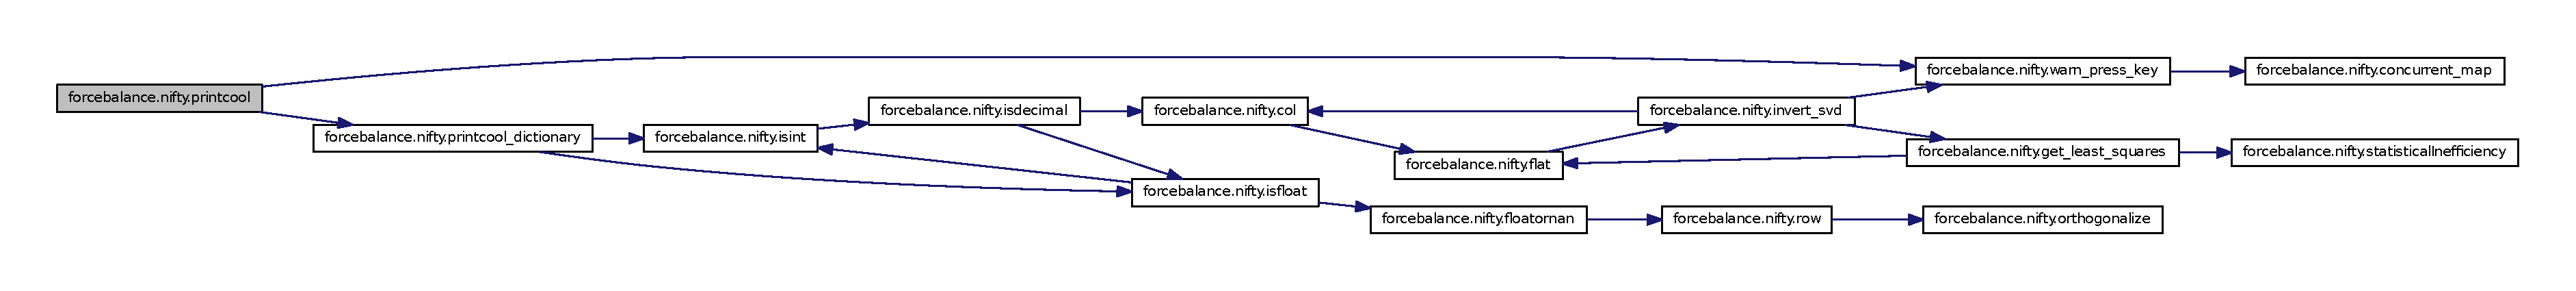
\includegraphics[width=350pt]{namespaceforcebalance_1_1nifty_a11babd62dc7bca389162c6318f9672ca_cgraph}
\end{center}
\end{figure}


\hypertarget{namespaceforcebalance_1_1nifty_a51180e960742cc7547749fdfb3513ec4}{\index{forcebalance\-::nifty@{forcebalance\-::nifty}!printcool\-\_\-dictionary@{printcool\-\_\-dictionary}}
\index{printcool\-\_\-dictionary@{printcool\-\_\-dictionary}!forcebalance::nifty@{forcebalance\-::nifty}}
\paragraph[{printcool\-\_\-dictionary}]{\setlength{\rightskip}{0pt plus 5cm}def forcebalance.\-nifty.\-printcool\-\_\-dictionary (
\begin{DoxyParamCaption}
\item[{}]{Dict, }
\item[{}]{title = {\ttfamily \char`\"{}General~options\char`\"{}}, }
\item[{}]{bold = {\ttfamily False}, }
\item[{}]{color = {\ttfamily 2}, }
\item[{}]{keywidth = {\ttfamily 25}, }
\item[{}]{topwidth = {\ttfamily 50}, }
\item[{}]{center = {\ttfamily True}, }
\item[{}]{leftpad = {\ttfamily 0}}
\end{DoxyParamCaption}
)}}\label{namespaceforcebalance_1_1nifty_a51180e960742cc7547749fdfb3513ec4}


See documentation for printcool; this is a nice way to print out keys/values in a dictionary. 

\begin{DoxyVerb} The keys in the dictionary are sorted before printing out.
\end{DoxyVerb}



\begin{DoxyParams}[1]{Parameters}
\mbox{\tt in}  & {\em dict} & The dictionary to be printed \\
\hline
\mbox{\tt in}  & {\em title} & The title of the printout \\
\hline
\end{DoxyParams}


Definition at line 197 of file nifty.\-py.



Here is the call graph for this function\-:\nopagebreak
\begin{figure}[H]
\begin{center}
\leavevmode
\includegraphics[width=350pt]{namespaceforcebalance_1_1nifty_a51180e960742cc7547749fdfb3513ec4_cgraph}
\end{center}
\end{figure}


\hypertarget{namespaceforcebalance_1_1nifty_a27e3a9dc144a5ad505509ac9ede08d7d}{\index{forcebalance\-::nifty@{forcebalance\-::nifty}!pvec1d@{pvec1d}}
\index{pvec1d@{pvec1d}!forcebalance::nifty@{forcebalance\-::nifty}}
\paragraph[{pvec1d}]{\setlength{\rightskip}{0pt plus 5cm}def forcebalance.\-nifty.\-pvec1d (
\begin{DoxyParamCaption}
\item[{}]{vec1d, }
\item[{}]{precision = {\ttfamily 1}, }
\item[{}]{loglevel = {\ttfamily forcebalance.output.INFO}}
\end{DoxyParamCaption}
)}}\label{namespaceforcebalance_1_1nifty_a27e3a9dc144a5ad505509ac9ede08d7d}


Printout of a 1-\/\-D vector. 


\begin{DoxyParams}[1]{Parameters}
\mbox{\tt in}  & {\em vec1d} & a 1-\/\-D vector \\
\hline
\end{DoxyParams}


Definition at line 54 of file nifty.\-py.



Here is the call graph for this function\-:\nopagebreak
\begin{figure}[H]
\begin{center}
\leavevmode
\includegraphics[width=350pt]{namespaceforcebalance_1_1nifty_a27e3a9dc144a5ad505509ac9ede08d7d_cgraph}
\end{center}
\end{figure}


\hypertarget{namespaceforcebalance_1_1nifty_a673f4a044169f5d8d822823989a836a7}{\index{forcebalance\-::nifty@{forcebalance\-::nifty}!queue\-\_\-up@{queue\-\_\-up}}
\index{queue\-\_\-up@{queue\-\_\-up}!forcebalance::nifty@{forcebalance\-::nifty}}
\paragraph[{queue\-\_\-up}]{\setlength{\rightskip}{0pt plus 5cm}def forcebalance.\-nifty.\-queue\-\_\-up (
\begin{DoxyParamCaption}
\item[{}]{wq, }
\item[{}]{command, }
\item[{}]{input\-\_\-files, }
\item[{}]{output\-\_\-files, }
\item[{}]{tgt = {\ttfamily None}, }
\item[{}]{verbose = {\ttfamily True}}
\end{DoxyParamCaption}
)}}\label{namespaceforcebalance_1_1nifty_a673f4a044169f5d8d822823989a836a7}


Submit a job to the Work Queue. 


\begin{DoxyParams}[1]{Parameters}
\mbox{\tt in}  & {\em wq} & (Work Queue Object) \\
\hline
\mbox{\tt in}  & {\em command} & (string) The command to run on the remote worker. \\
\hline
\mbox{\tt in}  & {\em input\-\_\-files} & (list of files) A list of locations of the input files. \\
\hline
\mbox{\tt in}  & {\em output\-\_\-files} & (list of files) A list of locations of the output files. \\
\hline
\end{DoxyParams}


Definition at line 589 of file nifty.\-py.



Here is the call graph for this function\-:\nopagebreak
\begin{figure}[H]
\begin{center}
\leavevmode
\includegraphics[width=350pt]{namespaceforcebalance_1_1nifty_a673f4a044169f5d8d822823989a836a7_cgraph}
\end{center}
\end{figure}


\hypertarget{namespaceforcebalance_1_1nifty_a5d5abeb4a185fde64721d044831e18ee}{\index{forcebalance\-::nifty@{forcebalance\-::nifty}!queue\-\_\-up\-\_\-src\-\_\-dest@{queue\-\_\-up\-\_\-src\-\_\-dest}}
\index{queue\-\_\-up\-\_\-src\-\_\-dest@{queue\-\_\-up\-\_\-src\-\_\-dest}!forcebalance::nifty@{forcebalance\-::nifty}}
\paragraph[{queue\-\_\-up\-\_\-src\-\_\-dest}]{\setlength{\rightskip}{0pt plus 5cm}def forcebalance.\-nifty.\-queue\-\_\-up\-\_\-src\-\_\-dest (
\begin{DoxyParamCaption}
\item[{}]{wq, }
\item[{}]{command, }
\item[{}]{input\-\_\-files, }
\item[{}]{output\-\_\-files, }
\item[{}]{tgt = {\ttfamily None}, }
\item[{}]{verbose = {\ttfamily True}}
\end{DoxyParamCaption}
)}}\label{namespaceforcebalance_1_1nifty_a5d5abeb4a185fde64721d044831e18ee}


Submit a job to the Work Queue. 

This function is a bit fancier in that we can explicitly specify where the input files come from, and where the output files go to.


\begin{DoxyParams}[1]{Parameters}
\mbox{\tt in}  & {\em wq} & (Work Queue Object) \\
\hline
\mbox{\tt in}  & {\em command} & (string) The command to run on the remote worker. \\
\hline
\mbox{\tt in}  & {\em input\-\_\-files} & (list of 2-\/tuples) A list of local and remote locations of the input files. \\
\hline
\mbox{\tt in}  & {\em output\-\_\-files} & (list of 2-\/tuples) A list of local and remote locations of the output files. \\
\hline
\end{DoxyParams}


Definition at line 620 of file nifty.\-py.

\hypertarget{namespaceforcebalance_1_1nifty_a25efa4d501ad852a234721af18978f7e}{\index{forcebalance\-::nifty@{forcebalance\-::nifty}!remove\-\_\-if\-\_\-exists@{remove\-\_\-if\-\_\-exists}}
\index{remove\-\_\-if\-\_\-exists@{remove\-\_\-if\-\_\-exists}!forcebalance::nifty@{forcebalance\-::nifty}}
\paragraph[{remove\-\_\-if\-\_\-exists}]{\setlength{\rightskip}{0pt plus 5cm}def forcebalance.\-nifty.\-remove\-\_\-if\-\_\-exists (
\begin{DoxyParamCaption}
\item[{}]{fnm}
\end{DoxyParamCaption}
)}}\label{namespaceforcebalance_1_1nifty_a25efa4d501ad852a234721af18978f7e}


Remove the file if it exists (doesn't return an error). 



Definition at line 775 of file nifty.\-py.

\hypertarget{namespaceforcebalance_1_1nifty_a6c9727360cdff8f3011a12cc54d0e86e}{\index{forcebalance\-::nifty@{forcebalance\-::nifty}!row@{row}}
\index{row@{row}!forcebalance::nifty@{forcebalance\-::nifty}}
\paragraph[{row}]{\setlength{\rightskip}{0pt plus 5cm}def forcebalance.\-nifty.\-row (
\begin{DoxyParamCaption}
\item[{}]{vec}
\end{DoxyParamCaption}
)}}\label{namespaceforcebalance_1_1nifty_a6c9727360cdff8f3011a12cc54d0e86e}


Given any list, array, or matrix, return a 1-\/row matrix. 


\begin{DoxyParams}[1]{Parameters}
\mbox{\tt in}  & {\em vec} & The input vector that is to be made into a row\\
\hline
\end{DoxyParams}
\begin{DoxyReturn}{Returns}
answer A row matrix 
\end{DoxyReturn}


Definition at line 280 of file nifty.\-py.



Here is the call graph for this function\-:\nopagebreak
\begin{figure}[H]
\begin{center}
\leavevmode
\includegraphics[width=350pt]{namespaceforcebalance_1_1nifty_a6c9727360cdff8f3011a12cc54d0e86e_cgraph}
\end{center}
\end{figure}


\hypertarget{namespaceforcebalance_1_1nifty_a3b9fd8e29c5d8f1b2114e4d9662dfd61}{\index{forcebalance\-::nifty@{forcebalance\-::nifty}!segments@{segments}}
\index{segments@{segments}!forcebalance::nifty@{forcebalance\-::nifty}}
\paragraph[{segments}]{\setlength{\rightskip}{0pt plus 5cm}def forcebalance.\-nifty.\-segments (
\begin{DoxyParamCaption}
\item[{}]{e}
\end{DoxyParamCaption}
)}}\label{namespaceforcebalance_1_1nifty_a3b9fd8e29c5d8f1b2114e4d9662dfd61}


Definition at line 75 of file nifty.\-py.



Here is the call graph for this function\-:\nopagebreak
\begin{figure}[H]
\begin{center}
\leavevmode
\includegraphics[width=350pt]{namespaceforcebalance_1_1nifty_a3b9fd8e29c5d8f1b2114e4d9662dfd61_cgraph}
\end{center}
\end{figure}


\hypertarget{namespaceforcebalance_1_1nifty_ad5ca60565c864b4245a8212fe9d92e10}{\index{forcebalance\-::nifty@{forcebalance\-::nifty}!statistical\-Inefficiency@{statistical\-Inefficiency}}
\index{statistical\-Inefficiency@{statistical\-Inefficiency}!forcebalance::nifty@{forcebalance\-::nifty}}
\paragraph[{statistical\-Inefficiency}]{\setlength{\rightskip}{0pt plus 5cm}def forcebalance.\-nifty.\-statistical\-Inefficiency (
\begin{DoxyParamCaption}
\item[{}]{A\-\_\-n, }
\item[{}]{B\-\_\-n = {\ttfamily None}, }
\item[{}]{fast = {\ttfamily False}, }
\item[{}]{mintime = {\ttfamily 3}, }
\item[{}]{warn = {\ttfamily True}}
\end{DoxyParamCaption}
)}}\label{namespaceforcebalance_1_1nifty_ad5ca60565c864b4245a8212fe9d92e10}


Compute the (cross) statistical inefficiency of (two) timeseries. 

\begin{DoxyVerb} Notes
   The same timeseries can be used for both A_n and B_n to get the autocorrelation statistical inefficiency.
   The fast method described in Ref [1] is used to compute g.

 References
   [1] J. D. Chodera, W. C. Swope, J. W. Pitera, C. Seok, and K. A. Dill. Use of the weighted
   histogram analysis method for the analysis of simulated and parallel tempering simulations.
   JCTC 3(1):26-41, 2007.

 Examples

 Compute statistical inefficiency of timeseries data with known correlation time.

 >>> import timeseries
 >>> A_n = timeseries.generateCorrelatedTimeseries(N=100000, tau=5.0)
 >>> g = statisticalInefficiency(A_n, fast=True)
\end{DoxyVerb}



\begin{DoxyParams}[1]{Parameters}
\mbox{\tt in}  & {\em A\-\_\-n} & (required, numpy array) -\/ A\-\_\-n\mbox{[}n\mbox{]} is nth value of timeseries A. Length is deduced from vector.\\
\hline
\mbox{\tt in}  & {\em B\-\_\-n} & (optional, numpy array) -\/ B\-\_\-n\mbox{[}n\mbox{]} is nth value of timeseries B. Length is deduced from vector. If supplied, the cross-\/correlation of timeseries A and B will be estimated instead of the autocorrelation of timeseries A.\\
\hline
\mbox{\tt in}  & {\em fast} & (optional, boolean) -\/ if True, will use faster (but less accurate) method to estimate correlation time, described in Ref. \mbox{[}1\mbox{]} (default\-: False)\\
\hline
\mbox{\tt in}  & {\em mintime} & (optional, int) -\/ minimum amount of correlation function to compute (default\-: 3) The algorithm terminates after computing the correlation time out to mintime when the correlation function furst goes negative. Note that this time may need to be increased if there is a strong initial negative peak in the correlation function.\\
\hline
\end{DoxyParams}
\begin{DoxyReturn}{Returns}
g The estimated statistical inefficiency (equal to 1 + 2 tau, where tau is the correlation time). We enforce g $>$= 1.\-0. 
\end{DoxyReturn}


Definition at line 433 of file nifty.\-py.

\hypertarget{namespaceforcebalance_1_1nifty_afa670d68f01813ac8d429bc5cbdb4f9f}{\index{forcebalance\-::nifty@{forcebalance\-::nifty}!uncommadash@{uncommadash}}
\index{uncommadash@{uncommadash}!forcebalance::nifty@{forcebalance\-::nifty}}
\paragraph[{uncommadash}]{\setlength{\rightskip}{0pt plus 5cm}def forcebalance.\-nifty.\-uncommadash (
\begin{DoxyParamCaption}
\item[{}]{s}
\end{DoxyParamCaption}
)}}\label{namespaceforcebalance_1_1nifty_afa670d68f01813ac8d429bc5cbdb4f9f}


Definition at line 91 of file nifty.\-py.



Here is the call graph for this function\-:\nopagebreak
\begin{figure}[H]
\begin{center}
\leavevmode
\includegraphics[width=350pt]{namespaceforcebalance_1_1nifty_afa670d68f01813ac8d429bc5cbdb4f9f_cgraph}
\end{center}
\end{figure}


\hypertarget{namespaceforcebalance_1_1nifty_a26e563ec71ed229c30f3d61d3448c8f1}{\index{forcebalance\-::nifty@{forcebalance\-::nifty}!warn\-\_\-once@{warn\-\_\-once}}
\index{warn\-\_\-once@{warn\-\_\-once}!forcebalance::nifty@{forcebalance\-::nifty}}
\paragraph[{warn\-\_\-once}]{\setlength{\rightskip}{0pt plus 5cm}def forcebalance.\-nifty.\-warn\-\_\-once (
\begin{DoxyParamCaption}
\item[{}]{warning, }
\item[{}]{warnhash = {\ttfamily None}}
\end{DoxyParamCaption}
)}}\label{namespaceforcebalance_1_1nifty_a26e563ec71ed229c30f3d61d3448c8f1}


Prints a warning but will only do so once in a given run. 



Definition at line 887 of file nifty.\-py.



Here is the call graph for this function\-:\nopagebreak
\begin{figure}[H]
\begin{center}
\leavevmode
\includegraphics[width=350pt]{namespaceforcebalance_1_1nifty_a26e563ec71ed229c30f3d61d3448c8f1_cgraph}
\end{center}
\end{figure}


\hypertarget{namespaceforcebalance_1_1nifty_abb8f59044961a12588e0653c2baa8b01}{\index{forcebalance\-::nifty@{forcebalance\-::nifty}!warn\-\_\-press\-\_\-key@{warn\-\_\-press\-\_\-key}}
\index{warn\-\_\-press\-\_\-key@{warn\-\_\-press\-\_\-key}!forcebalance::nifty@{forcebalance\-::nifty}}
\paragraph[{warn\-\_\-press\-\_\-key}]{\setlength{\rightskip}{0pt plus 5cm}def forcebalance.\-nifty.\-warn\-\_\-press\-\_\-key (
\begin{DoxyParamCaption}
\item[{}]{warning, }
\item[{}]{timeout = {\ttfamily 10}}
\end{DoxyParamCaption}
)}}\label{namespaceforcebalance_1_1nifty_abb8f59044961a12588e0653c2baa8b01}


Definition at line 872 of file nifty.\-py.



Here is the call graph for this function\-:\nopagebreak
\begin{figure}[H]
\begin{center}
\leavevmode
\includegraphics[width=350pt]{namespaceforcebalance_1_1nifty_abb8f59044961a12588e0653c2baa8b01_cgraph}
\end{center}
\end{figure}


\hypertarget{namespaceforcebalance_1_1nifty_aa1ff334c4b4e30e91978b91d9a9ec065}{\index{forcebalance\-::nifty@{forcebalance\-::nifty}!which@{which}}
\index{which@{which}!forcebalance::nifty@{forcebalance\-::nifty}}
\paragraph[{which}]{\setlength{\rightskip}{0pt plus 5cm}def forcebalance.\-nifty.\-which (
\begin{DoxyParamCaption}
\item[{}]{fnm}
\end{DoxyParamCaption}
)}}\label{namespaceforcebalance_1_1nifty_aa1ff334c4b4e30e91978b91d9a9ec065}


Definition at line 779 of file nifty.\-py.



Here is the call graph for this function\-:\nopagebreak
\begin{figure}[H]
\begin{center}
\leavevmode
\includegraphics[width=350pt]{namespaceforcebalance_1_1nifty_aa1ff334c4b4e30e91978b91d9a9ec065_cgraph}
\end{center}
\end{figure}


\hypertarget{namespaceforcebalance_1_1nifty_a576de8c5b6f236280e07e73e39b2ab7c}{\index{forcebalance\-::nifty@{forcebalance\-::nifty}!wq\-\_\-wait@{wq\-\_\-wait}}
\index{wq\-\_\-wait@{wq\-\_\-wait}!forcebalance::nifty@{forcebalance\-::nifty}}
\paragraph[{wq\-\_\-wait}]{\setlength{\rightskip}{0pt plus 5cm}def forcebalance.\-nifty.\-wq\-\_\-wait (
\begin{DoxyParamCaption}
\item[{}]{wq, }
\item[{}]{verbose = {\ttfamily False}}
\end{DoxyParamCaption}
)}}\label{namespaceforcebalance_1_1nifty_a576de8c5b6f236280e07e73e39b2ab7c}


This function waits until the work queue is completely empty. 



Definition at line 691 of file nifty.\-py.



Here is the call graph for this function\-:\nopagebreak
\begin{figure}[H]
\begin{center}
\leavevmode
\includegraphics[width=350pt]{namespaceforcebalance_1_1nifty_a576de8c5b6f236280e07e73e39b2ab7c_cgraph}
\end{center}
\end{figure}


\hypertarget{namespaceforcebalance_1_1nifty_a374aac2ef003be02fab49b20ff0a82f0}{\index{forcebalance\-::nifty@{forcebalance\-::nifty}!wq\-\_\-wait1@{wq\-\_\-wait1}}
\index{wq\-\_\-wait1@{wq\-\_\-wait1}!forcebalance::nifty@{forcebalance\-::nifty}}
\paragraph[{wq\-\_\-wait1}]{\setlength{\rightskip}{0pt plus 5cm}def forcebalance.\-nifty.\-wq\-\_\-wait1 (
\begin{DoxyParamCaption}
\item[{}]{wq, }
\item[{}]{wait\-\_\-time = {\ttfamily 10}, }
\item[{}]{verbose = {\ttfamily False}}
\end{DoxyParamCaption}
)}}\label{namespaceforcebalance_1_1nifty_a374aac2ef003be02fab49b20ff0a82f0}


This function waits ten seconds to see if a task in the Work Queue has finished. 



Definition at line 640 of file nifty.\-py.



Here is the call graph for this function\-:\nopagebreak
\begin{figure}[H]
\begin{center}
\leavevmode
\includegraphics[width=350pt]{namespaceforcebalance_1_1nifty_a374aac2ef003be02fab49b20ff0a82f0_cgraph}
\end{center}
\end{figure}




\subsubsection{Variable Documentation}
\hypertarget{namespaceforcebalance_1_1nifty_a31a8d4a4240a1325bd4fa10033b7eee0}{\index{forcebalance\-::nifty@{forcebalance\-::nifty}!bohrang@{bohrang}}
\index{bohrang@{bohrang}!forcebalance::nifty@{forcebalance\-::nifty}}
\paragraph[{bohrang}]{\setlength{\rightskip}{0pt plus 5cm}float forcebalance.\-nifty.\-bohrang = 0.\-529177249}}\label{namespaceforcebalance_1_1nifty_a31a8d4a4240a1325bd4fa10033b7eee0}


One bohr equals this many angstroms. 



Definition at line 44 of file nifty.\-py.

\hypertarget{namespaceforcebalance_1_1nifty_a7cec4d46378b888cd867de05d0168d96}{\index{forcebalance\-::nifty@{forcebalance\-::nifty}!eqcgmx@{eqcgmx}}
\index{eqcgmx@{eqcgmx}!forcebalance::nifty@{forcebalance\-::nifty}}
\paragraph[{eqcgmx}]{\setlength{\rightskip}{0pt plus 5cm}float forcebalance.\-nifty.\-eqcgmx = 2625.\-5002}}\label{namespaceforcebalance_1_1nifty_a7cec4d46378b888cd867de05d0168d96}


Q-\/\-Chem to G\-M\-X unit conversion for energy. 



Definition at line 40 of file nifty.\-py.

\hypertarget{namespaceforcebalance_1_1nifty_ab1ec21beaae0d8328e7e4c3b89d972ab}{\index{forcebalance\-::nifty@{forcebalance\-::nifty}!fqcgmx@{fqcgmx}}
\index{fqcgmx@{fqcgmx}!forcebalance::nifty@{forcebalance\-::nifty}}
\paragraph[{fqcgmx}]{\setlength{\rightskip}{0pt plus 5cm}float forcebalance.\-nifty.\-fqcgmx = -\/49621.\-9}}\label{namespaceforcebalance_1_1nifty_ab1ec21beaae0d8328e7e4c3b89d972ab}


Q-\/\-Chem to G\-M\-X unit conversion for force. 



Definition at line 42 of file nifty.\-py.

\hypertarget{namespaceforcebalance_1_1nifty_ae0916a3186f4f8b238a0d58bb9f6a3da}{\index{forcebalance\-::nifty@{forcebalance\-::nifty}!kb@{kb}}
\index{kb@{kb}!forcebalance::nifty@{forcebalance\-::nifty}}
\paragraph[{kb}]{\setlength{\rightskip}{0pt plus 5cm}float forcebalance.\-nifty.\-kb = 0.\-0083144100163}}\label{namespaceforcebalance_1_1nifty_ae0916a3186f4f8b238a0d58bb9f6a3da}


Boltzmann constant. 



Definition at line 38 of file nifty.\-py.

\hypertarget{namespaceforcebalance_1_1nifty_a1859e992ed983dbbcc8093fdd19710e7}{\index{forcebalance\-::nifty@{forcebalance\-::nifty}!logger@{logger}}
\index{logger@{logger}!forcebalance::nifty@{forcebalance\-::nifty}}
\paragraph[{logger}]{\setlength{\rightskip}{0pt plus 5cm}tuple forcebalance.\-nifty.\-logger = get\-Logger(\-\_\-\-\_\-name\-\_\-\-\_\-)}}\label{namespaceforcebalance_1_1nifty_a1859e992ed983dbbcc8093fdd19710e7}


Definition at line 34 of file nifty.\-py.

\hypertarget{namespaceforcebalance_1_1nifty_ab652c941890b0f378100433699c8d255}{\index{forcebalance\-::nifty@{forcebalance\-::nifty}!specific\-\_\-dct@{specific\-\_\-dct}}
\index{specific\-\_\-dct@{specific\-\_\-dct}!forcebalance::nifty@{forcebalance\-::nifty}}
\paragraph[{specific\-\_\-dct}]{\setlength{\rightskip}{0pt plus 5cm}tuple forcebalance.\-nifty.\-specific\-\_\-dct = dict(list(itertools.\-chain($\ast$\mbox{[}\mbox{[}(j,i\mbox{[}1\mbox{]}) for j in i\mbox{[}0\mbox{]}\mbox{]} for i in {\bf specific\-\_\-lst}\mbox{]})))}}\label{namespaceforcebalance_1_1nifty_ab652c941890b0f378100433699c8d255}


Definition at line 731 of file nifty.\-py.

\hypertarget{namespaceforcebalance_1_1nifty_abe850bcdf26cec4a0cf913a54a7ddfaa}{\index{forcebalance\-::nifty@{forcebalance\-::nifty}!specific\-\_\-lst@{specific\-\_\-lst}}
\index{specific\-\_\-lst@{specific\-\_\-lst}!forcebalance::nifty@{forcebalance\-::nifty}}
\paragraph[{specific\-\_\-lst}]{\setlength{\rightskip}{0pt plus 5cm}list forcebalance.\-nifty.\-specific\-\_\-lst}}\label{namespaceforcebalance_1_1nifty_abe850bcdf26cec4a0cf913a54a7ddfaa}
{\bfseries Initial value\-:}
\begin{DoxyCode}
1 = [([\textcolor{stringliteral}{'mdrun'},\textcolor{stringliteral}{'grompp'},\textcolor{stringliteral}{'trjconv'},\textcolor{stringliteral}{'g\_energy'},\textcolor{stringliteral}{'g\_traj'}], \textcolor{stringliteral}{"Make sure to install GROMACS and add it to your path
       (or set the gmxpath option)"}),
2                 ([\textcolor{stringliteral}{'force.mdin'}, \textcolor{stringliteral}{'stage.leap'}], \textcolor{stringliteral}{"This file is needed for setting up AMBER force matching
       targets"}),
3                 ([\textcolor{stringliteral}{'conf.pdb'}, \textcolor{stringliteral}{'mono.pdb'}], \textcolor{stringliteral}{"This file is needed for setting up OpenMM condensed phase
       property targets"}),
4                 ([\textcolor{stringliteral}{'liquid.xyz'}, \textcolor{stringliteral}{'liquid.key'}, \textcolor{stringliteral}{'mono.xyz'}, \textcolor{stringliteral}{'mono.key'}], \textcolor{stringliteral}{"This file is needed for setting up
       OpenMM condensed phase property targets"}),
5                 ([\textcolor{stringliteral}{'dynamic'}, \textcolor{stringliteral}{'analyze'}, \textcolor{stringliteral}{'minimize'}, \textcolor{stringliteral}{'testgrad'}, \textcolor{stringliteral}{'vibrate'}, \textcolor{stringliteral}{'optimize'}, \textcolor{stringliteral}{'polarize'}, \textcolor{stringliteral}{'
      superpose'}], \textcolor{stringliteral}{"Make sure to install TINKER and add it to your path (or set the tinkerpath option)"}),
6                 ([\textcolor{stringliteral}{'runcuda.sh'}, \textcolor{stringliteral}{'npt.py'}, \textcolor{stringliteral}{'npt\_tinker.py'}], \textcolor{stringliteral}{"This file belongs in the ForceBalance source
       directory, not sure why it is missing"}),
7                 ([\textcolor{stringliteral}{'input.xyz'}], \textcolor{stringliteral}{"This file is needed for TINKER molecular property targets"}),
8                 ([\textcolor{stringliteral}{'.*key$'}, \textcolor{stringliteral}{'.*xyz$'}], \textcolor{stringliteral}{"I am guessing this file is probably needed by TINKER"}),
9                 ([\textcolor{stringliteral}{'.*gro$'}, \textcolor{stringliteral}{'.*top$'}, \textcolor{stringliteral}{'.*itp$'}, \textcolor{stringliteral}{'.*mdp$'}, \textcolor{stringliteral}{'.*ndx$'}], \textcolor{stringliteral}{"I am guessing this file is probably
       needed by GROMACS"})
10                 ]
\end{DoxyCode}


Definition at line 719 of file nifty.\-py.

\hypertarget{namespaceforcebalance_1_1nifty_a338d5080f95188c37271c306f64093d8}{\index{forcebalance\-::nifty@{forcebalance\-::nifty}!X\-M\-L\-F\-I\-L\-E@{X\-M\-L\-F\-I\-L\-E}}
\index{X\-M\-L\-F\-I\-L\-E@{X\-M\-L\-F\-I\-L\-E}!forcebalance::nifty@{forcebalance\-::nifty}}
\paragraph[{X\-M\-L\-F\-I\-L\-E}]{\setlength{\rightskip}{0pt plus 5cm}string forcebalance.\-nifty.\-X\-M\-L\-F\-I\-L\-E = 'x'}}\label{namespaceforcebalance_1_1nifty_a338d5080f95188c37271c306f64093d8}


Pickle uses 'flags' to pickle and unpickle different variable types. 

Here we use the letter 'x' to signify that the variable type is an X\-M\-L file. 

Definition at line 495 of file nifty.\-py.


\hypertarget{namespaceforcebalance_1_1objective}{\subsection{forcebalance\-:\-:objective \-Namespace \-Reference}
\label{namespaceforcebalance_1_1objective}\index{forcebalance\-::objective@{forcebalance\-::objective}}
}


\-Force\-Balance objective function.  


\subsubsection*{\-Classes}
\begin{DoxyCompactItemize}
\item 
class \hyperlink{classforcebalance_1_1objective_1_1Objective}{\-Objective}
\begin{DoxyCompactList}\small\item\em \hyperlink{classforcebalance_1_1objective_1_1Objective}{\-Objective} function. \end{DoxyCompactList}\item 
class \hyperlink{classforcebalance_1_1objective_1_1Penalty}{\-Penalty}
\begin{DoxyCompactList}\small\item\em \hyperlink{classforcebalance_1_1objective_1_1Penalty}{\-Penalty} functions for regularizing the force field optimizer. \end{DoxyCompactList}\end{DoxyCompactItemize}
\subsubsection*{\-Variables}
\begin{DoxyCompactItemize}
\item 
tuple \hyperlink{namespaceforcebalance_1_1objective_afa1d976cc1f8b18cf0b03f1ccf49f590}{logger} = get\-Logger(\-\_\-\-\_\-name\-\_\-\-\_\-)
\item 
dictionary \hyperlink{namespaceforcebalance_1_1objective_aad3b66466fd22980d2c83c67b82ddddf}{\-Implemented\-\_\-\-Targets}
\begin{DoxyCompactList}\small\item\em \-The table of implemented \-Targets. \end{DoxyCompactList}\item 
list \hyperlink{namespaceforcebalance_1_1objective_a01660ebc02853011e66350c410e26f0a}{\-Letters} = \mbox{[}'\-X','\-G','\-H'\mbox{]}
\begin{DoxyCompactList}\small\item\em \-This is the canonical lettering that corresponds to \-: objective function, gradient, \-Hessian. \end{DoxyCompactList}\end{DoxyCompactItemize}


\subsubsection{\-Detailed \-Description}
\-Force\-Balance objective function. 

\subsubsection{\-Variable \-Documentation}
\hypertarget{namespaceforcebalance_1_1objective_aad3b66466fd22980d2c83c67b82ddddf}{\index{forcebalance\-::objective@{forcebalance\-::objective}!\-Implemented\-\_\-\-Targets@{\-Implemented\-\_\-\-Targets}}
\index{\-Implemented\-\_\-\-Targets@{\-Implemented\-\_\-\-Targets}!forcebalance::objective@{forcebalance\-::objective}}
\paragraph[{\-Implemented\-\_\-\-Targets}]{\setlength{\rightskip}{0pt plus 5cm}dictionary {\bf forcebalance\-::objective\-::\-Implemented\-\_\-\-Targets}}}\label{namespaceforcebalance_1_1objective_aad3b66466fd22980d2c83c67b82ddddf}
{\bfseries \-Initial value\-:}
\begin{DoxyCode}
1 {
2     'ABINITIO_GMX':AbInitio_GMX,
3     'ABINITIO_TINKER':AbInitio_TINKER,
4     'ABINITIO_OPENMM':AbInitio_OpenMM,
5     'ABINITIO_AMBER':AbInitio_AMBER,
6     'ABINITIO_INTERNAL':AbInitio_Internal,
7     'VIBRATION_TINKER':Vibration_TINKER,
8     'LIQUID_OPENMM':Liquid_OpenMM,
9     'LIQUID_TINKER':Liquid_TINKER, 
10     'LIQUID_GMX':Liquid_GMX, 
11     'COUNTERPOISE':Counterpoise,
12     'THCDF_PSI4':THCDF_Psi4,
13     'RDVR3_PSI4':RDVR3_Psi4,
14     'INTERACTION_TINKER':Interaction_TINKER,
15     'INTERACTION_OPENMM':Interaction_OpenMM,
16     'BINDINGENERGY_TINKER':BindingEnergy_TINKER,
17     'MOMENTS_TINKER':Moments_TINKER,
18     'MONOMER_QTPIE':Monomer_QTPIE,
19     }
\end{DoxyCode}


\-The table of implemented \-Targets. 



\-Definition at line 68 of file objective.\-py.

\hypertarget{namespaceforcebalance_1_1objective_a01660ebc02853011e66350c410e26f0a}{\index{forcebalance\-::objective@{forcebalance\-::objective}!\-Letters@{\-Letters}}
\index{\-Letters@{\-Letters}!forcebalance::objective@{forcebalance\-::objective}}
\paragraph[{\-Letters}]{\setlength{\rightskip}{0pt plus 5cm}list {\bf forcebalance\-::objective\-::\-Letters} = \mbox{[}'\-X','\-G','\-H'\mbox{]}}}\label{namespaceforcebalance_1_1objective_a01660ebc02853011e66350c410e26f0a}


\-This is the canonical lettering that corresponds to \-: objective function, gradient, \-Hessian. 



\-Definition at line 89 of file objective.\-py.

\hypertarget{namespaceforcebalance_1_1objective_afa1d976cc1f8b18cf0b03f1ccf49f590}{\index{forcebalance\-::objective@{forcebalance\-::objective}!logger@{logger}}
\index{logger@{logger}!forcebalance::objective@{forcebalance\-::objective}}
\paragraph[{logger}]{\setlength{\rightskip}{0pt plus 5cm}tuple {\bf forcebalance\-::objective\-::logger} = get\-Logger(\-\_\-\-\_\-name\-\_\-\-\_\-)}}\label{namespaceforcebalance_1_1objective_afa1d976cc1f8b18cf0b03f1ccf49f590}


\-Definition at line 17 of file objective.\-py.


\hypertarget{namespaceforcebalance_1_1openmmio}{\subsection{forcebalance.\-openmmio Namespace Reference}
\label{namespaceforcebalance_1_1openmmio}\index{forcebalance.\-openmmio@{forcebalance.\-openmmio}}
}


Open\-M\-M input/output.  


\subsubsection*{Classes}
\begin{DoxyCompactItemize}
\item 
class \hyperlink{classforcebalance_1_1openmmio_1_1OpenMM__Reader}{Open\-M\-M\-\_\-\-Reader}
\begin{DoxyCompactList}\small\item\em Class for parsing Open\-M\-M force field files. \end{DoxyCompactList}\item 
class \hyperlink{classforcebalance_1_1openmmio_1_1Liquid__OpenMM}{Liquid\-\_\-\-Open\-M\-M}
\item 
class \hyperlink{classforcebalance_1_1openmmio_1_1AbInitio__OpenMM}{Ab\-Initio\-\_\-\-Open\-M\-M}
\begin{DoxyCompactList}\small\item\em Subclass of Ab\-Initio for force and energy matching using Open\-M\-M. \end{DoxyCompactList}\item 
class \hyperlink{classforcebalance_1_1openmmio_1_1Interaction__OpenMM}{Interaction\-\_\-\-Open\-M\-M}
\begin{DoxyCompactList}\small\item\em Subclass of Target for interaction matching using Open\-M\-M. \end{DoxyCompactList}\end{DoxyCompactItemize}
\subsubsection*{Functions}
\begin{DoxyCompactItemize}
\item 
def \hyperlink{namespaceforcebalance_1_1openmmio_a8a2081dcaf027b9b9ab224e22680714d}{get\-\_\-dipole}
\begin{DoxyCompactList}\small\item\em Return the current dipole moment in Debye. \end{DoxyCompactList}\item 
def \hyperlink{namespaceforcebalance_1_1openmmio_af623fa5af97de6c6a0bc5f98ce8db432}{Reset\-Virtual\-Sites}
\begin{DoxyCompactList}\small\item\em Given a set of Open\-M\-M-\/compatible positions and a System object, compute the correct virtual site positions according to the System. \end{DoxyCompactList}\item 
def \hyperlink{namespaceforcebalance_1_1openmmio_a792a195b31612f2140b35927fe28fa1a}{Copy\-Amoeba\-Bond\-Parameters}
\item 
def \hyperlink{namespaceforcebalance_1_1openmmio_a2e95f600757655d41660c25af8fd8e80}{Copy\-Amoeba\-Out\-Of\-Plane\-Bend\-Parameters}
\item 
def \hyperlink{namespaceforcebalance_1_1openmmio_abe9a6b9b200dc8487e56dad7249af3ec}{Copy\-Amoeba\-Angle\-Parameters}
\item 
def \hyperlink{namespaceforcebalance_1_1openmmio_ad0d4739f80f2aab1a861f2e03b8efcd6}{Copy\-Amoeba\-In\-Plane\-Angle\-Parameters}
\item 
def \hyperlink{namespaceforcebalance_1_1openmmio_abe005f73c6dfe9ce1052c9434bcad9be}{Copy\-Amoeba\-Vdw\-Parameters}
\item 
def \hyperlink{namespaceforcebalance_1_1openmmio_a3706c19e71969cabe5782a4535abeffe}{Copy\-Amoeba\-Multipole\-Parameters}
\item 
def \hyperlink{namespaceforcebalance_1_1openmmio_a616f12cc53381716e5fa41f00bf623be}{Copy\-Harmonic\-Bond\-Parameters}
\item 
def \hyperlink{namespaceforcebalance_1_1openmmio_af4ed16f5e2b1cd12bce2f25fab1b05bc}{Copy\-Harmonic\-Angle\-Parameters}
\item 
def \hyperlink{namespaceforcebalance_1_1openmmio_a8f13702754f0b4e43e272139a2ce8341}{Copy\-Periodic\-Torsion\-Parameters}
\item 
def \hyperlink{namespaceforcebalance_1_1openmmio_afead47464a644d9225f9fa8eb568a8ed}{Copy\-Nonbonded\-Parameters}
\item 
def \hyperlink{namespaceforcebalance_1_1openmmio_a2bb7add6b813d94f2655372c51fe8fdc}{do\-\_\-nothing}
\item 
def \hyperlink{namespaceforcebalance_1_1openmmio_a8c6ed589ec2b35b8363a529ffdf88eb0}{Copy\-System\-Parameters}
\begin{DoxyCompactList}\small\item\em Copy parameters from one system (i.\-e. \end{DoxyCompactList}\item 
def \hyperlink{namespaceforcebalance_1_1openmmio_a9f9fc56475dbfcc94a40fef6a84ed25f}{Update\-Simulation\-Parameters}
\item 
def \hyperlink{namespaceforcebalance_1_1openmmio_aa085594c11e9cd00ce71f5a8ead72b68}{M\-T\-S\-V\-V\-V\-R\-Integrator}
\begin{DoxyCompactList}\small\item\em Create a multiple timestep velocity verlet with velocity randomization (V\-V\-V\-R) integrator. \end{DoxyCompactList}\end{DoxyCompactItemize}
\subsubsection*{Variables}
\begin{DoxyCompactItemize}
\item 
dictionary \hyperlink{namespaceforcebalance_1_1openmmio_aeca37c08912f1a88339680ed75839530}{suffix\-\_\-dict}
\item 
string \hyperlink{namespaceforcebalance_1_1openmmio_af225f2cfdcfd96ebd1d3175c8770a850}{pdict} = \char`\"{}X\-M\-L\-\_\-\-Override\char`\"{}
\begin{DoxyCompactList}\small\item\em pdict is a useless variable if the force field is X\-M\-L. \end{DoxyCompactList}\end{DoxyCompactItemize}


\subsubsection{Detailed Description}
Open\-M\-M input/output. \begin{DoxyAuthor}{Author}
Lee-\/\-Ping Wang 
\end{DoxyAuthor}
\begin{DoxyDate}{Date}
04/2012 
\end{DoxyDate}


\subsubsection{Function Documentation}
\hypertarget{namespaceforcebalance_1_1openmmio_abe9a6b9b200dc8487e56dad7249af3ec}{\index{forcebalance\-::openmmio@{forcebalance\-::openmmio}!Copy\-Amoeba\-Angle\-Parameters@{Copy\-Amoeba\-Angle\-Parameters}}
\index{Copy\-Amoeba\-Angle\-Parameters@{Copy\-Amoeba\-Angle\-Parameters}!forcebalance::openmmio@{forcebalance\-::openmmio}}
\paragraph[{Copy\-Amoeba\-Angle\-Parameters}]{\setlength{\rightskip}{0pt plus 5cm}def forcebalance.\-openmmio.\-Copy\-Amoeba\-Angle\-Parameters (
\begin{DoxyParamCaption}
\item[{}]{src, }
\item[{}]{dest}
\end{DoxyParamCaption}
)}}\label{namespaceforcebalance_1_1openmmio_abe9a6b9b200dc8487e56dad7249af3ec}


Definition at line 109 of file openmmio.\-py.



Here is the call graph for this function\-:\nopagebreak
\begin{figure}[H]
\begin{center}
\leavevmode
\includegraphics[width=350pt]{namespaceforcebalance_1_1openmmio_abe9a6b9b200dc8487e56dad7249af3ec_cgraph}
\end{center}
\end{figure}


\hypertarget{namespaceforcebalance_1_1openmmio_a792a195b31612f2140b35927fe28fa1a}{\index{forcebalance\-::openmmio@{forcebalance\-::openmmio}!Copy\-Amoeba\-Bond\-Parameters@{Copy\-Amoeba\-Bond\-Parameters}}
\index{Copy\-Amoeba\-Bond\-Parameters@{Copy\-Amoeba\-Bond\-Parameters}!forcebalance::openmmio@{forcebalance\-::openmmio}}
\paragraph[{Copy\-Amoeba\-Bond\-Parameters}]{\setlength{\rightskip}{0pt plus 5cm}def forcebalance.\-openmmio.\-Copy\-Amoeba\-Bond\-Parameters (
\begin{DoxyParamCaption}
\item[{}]{src, }
\item[{}]{dest}
\end{DoxyParamCaption}
)}}\label{namespaceforcebalance_1_1openmmio_a792a195b31612f2140b35927fe28fa1a}


Definition at line 95 of file openmmio.\-py.



Here is the call graph for this function\-:\nopagebreak
\begin{figure}[H]
\begin{center}
\leavevmode
\includegraphics[width=350pt]{namespaceforcebalance_1_1openmmio_a792a195b31612f2140b35927fe28fa1a_cgraph}
\end{center}
\end{figure}


\hypertarget{namespaceforcebalance_1_1openmmio_ad0d4739f80f2aab1a861f2e03b8efcd6}{\index{forcebalance\-::openmmio@{forcebalance\-::openmmio}!Copy\-Amoeba\-In\-Plane\-Angle\-Parameters@{Copy\-Amoeba\-In\-Plane\-Angle\-Parameters}}
\index{Copy\-Amoeba\-In\-Plane\-Angle\-Parameters@{Copy\-Amoeba\-In\-Plane\-Angle\-Parameters}!forcebalance::openmmio@{forcebalance\-::openmmio}}
\paragraph[{Copy\-Amoeba\-In\-Plane\-Angle\-Parameters}]{\setlength{\rightskip}{0pt plus 5cm}def forcebalance.\-openmmio.\-Copy\-Amoeba\-In\-Plane\-Angle\-Parameters (
\begin{DoxyParamCaption}
\item[{}]{src, }
\item[{}]{dest}
\end{DoxyParamCaption}
)}}\label{namespaceforcebalance_1_1openmmio_ad0d4739f80f2aab1a861f2e03b8efcd6}


Definition at line 118 of file openmmio.\-py.



Here is the call graph for this function\-:\nopagebreak
\begin{figure}[H]
\begin{center}
\leavevmode
\includegraphics[width=350pt]{namespaceforcebalance_1_1openmmio_ad0d4739f80f2aab1a861f2e03b8efcd6_cgraph}
\end{center}
\end{figure}


\hypertarget{namespaceforcebalance_1_1openmmio_a3706c19e71969cabe5782a4535abeffe}{\index{forcebalance\-::openmmio@{forcebalance\-::openmmio}!Copy\-Amoeba\-Multipole\-Parameters@{Copy\-Amoeba\-Multipole\-Parameters}}
\index{Copy\-Amoeba\-Multipole\-Parameters@{Copy\-Amoeba\-Multipole\-Parameters}!forcebalance::openmmio@{forcebalance\-::openmmio}}
\paragraph[{Copy\-Amoeba\-Multipole\-Parameters}]{\setlength{\rightskip}{0pt plus 5cm}def forcebalance.\-openmmio.\-Copy\-Amoeba\-Multipole\-Parameters (
\begin{DoxyParamCaption}
\item[{}]{src, }
\item[{}]{dest}
\end{DoxyParamCaption}
)}}\label{namespaceforcebalance_1_1openmmio_a3706c19e71969cabe5782a4535abeffe}


Definition at line 131 of file openmmio.\-py.



Here is the call graph for this function\-:\nopagebreak
\begin{figure}[H]
\begin{center}
\leavevmode
\includegraphics[width=350pt]{namespaceforcebalance_1_1openmmio_a3706c19e71969cabe5782a4535abeffe_cgraph}
\end{center}
\end{figure}


\hypertarget{namespaceforcebalance_1_1openmmio_a2e95f600757655d41660c25af8fd8e80}{\index{forcebalance\-::openmmio@{forcebalance\-::openmmio}!Copy\-Amoeba\-Out\-Of\-Plane\-Bend\-Parameters@{Copy\-Amoeba\-Out\-Of\-Plane\-Bend\-Parameters}}
\index{Copy\-Amoeba\-Out\-Of\-Plane\-Bend\-Parameters@{Copy\-Amoeba\-Out\-Of\-Plane\-Bend\-Parameters}!forcebalance::openmmio@{forcebalance\-::openmmio}}
\paragraph[{Copy\-Amoeba\-Out\-Of\-Plane\-Bend\-Parameters}]{\setlength{\rightskip}{0pt plus 5cm}def forcebalance.\-openmmio.\-Copy\-Amoeba\-Out\-Of\-Plane\-Bend\-Parameters (
\begin{DoxyParamCaption}
\item[{}]{src, }
\item[{}]{dest}
\end{DoxyParamCaption}
)}}\label{namespaceforcebalance_1_1openmmio_a2e95f600757655d41660c25af8fd8e80}


Definition at line 101 of file openmmio.\-py.



Here is the call graph for this function\-:\nopagebreak
\begin{figure}[H]
\begin{center}
\leavevmode
\includegraphics[width=350pt]{namespaceforcebalance_1_1openmmio_a2e95f600757655d41660c25af8fd8e80_cgraph}
\end{center}
\end{figure}


\hypertarget{namespaceforcebalance_1_1openmmio_abe005f73c6dfe9ce1052c9434bcad9be}{\index{forcebalance\-::openmmio@{forcebalance\-::openmmio}!Copy\-Amoeba\-Vdw\-Parameters@{Copy\-Amoeba\-Vdw\-Parameters}}
\index{Copy\-Amoeba\-Vdw\-Parameters@{Copy\-Amoeba\-Vdw\-Parameters}!forcebalance::openmmio@{forcebalance\-::openmmio}}
\paragraph[{Copy\-Amoeba\-Vdw\-Parameters}]{\setlength{\rightskip}{0pt plus 5cm}def forcebalance.\-openmmio.\-Copy\-Amoeba\-Vdw\-Parameters (
\begin{DoxyParamCaption}
\item[{}]{src, }
\item[{}]{dest}
\end{DoxyParamCaption}
)}}\label{namespaceforcebalance_1_1openmmio_abe005f73c6dfe9ce1052c9434bcad9be}


Definition at line 127 of file openmmio.\-py.



Here is the call graph for this function\-:\nopagebreak
\begin{figure}[H]
\begin{center}
\leavevmode
\includegraphics[width=350pt]{namespaceforcebalance_1_1openmmio_abe005f73c6dfe9ce1052c9434bcad9be_cgraph}
\end{center}
\end{figure}


\hypertarget{namespaceforcebalance_1_1openmmio_af4ed16f5e2b1cd12bce2f25fab1b05bc}{\index{forcebalance\-::openmmio@{forcebalance\-::openmmio}!Copy\-Harmonic\-Angle\-Parameters@{Copy\-Harmonic\-Angle\-Parameters}}
\index{Copy\-Harmonic\-Angle\-Parameters@{Copy\-Harmonic\-Angle\-Parameters}!forcebalance::openmmio@{forcebalance\-::openmmio}}
\paragraph[{Copy\-Harmonic\-Angle\-Parameters}]{\setlength{\rightskip}{0pt plus 5cm}def forcebalance.\-openmmio.\-Copy\-Harmonic\-Angle\-Parameters (
\begin{DoxyParamCaption}
\item[{}]{src, }
\item[{}]{dest}
\end{DoxyParamCaption}
)}}\label{namespaceforcebalance_1_1openmmio_af4ed16f5e2b1cd12bce2f25fab1b05bc}


Definition at line 139 of file openmmio.\-py.



Here is the call graph for this function\-:\nopagebreak
\begin{figure}[H]
\begin{center}
\leavevmode
\includegraphics[width=350pt]{namespaceforcebalance_1_1openmmio_af4ed16f5e2b1cd12bce2f25fab1b05bc_cgraph}
\end{center}
\end{figure}


\hypertarget{namespaceforcebalance_1_1openmmio_a616f12cc53381716e5fa41f00bf623be}{\index{forcebalance\-::openmmio@{forcebalance\-::openmmio}!Copy\-Harmonic\-Bond\-Parameters@{Copy\-Harmonic\-Bond\-Parameters}}
\index{Copy\-Harmonic\-Bond\-Parameters@{Copy\-Harmonic\-Bond\-Parameters}!forcebalance::openmmio@{forcebalance\-::openmmio}}
\paragraph[{Copy\-Harmonic\-Bond\-Parameters}]{\setlength{\rightskip}{0pt plus 5cm}def forcebalance.\-openmmio.\-Copy\-Harmonic\-Bond\-Parameters (
\begin{DoxyParamCaption}
\item[{}]{src, }
\item[{}]{dest}
\end{DoxyParamCaption}
)}}\label{namespaceforcebalance_1_1openmmio_a616f12cc53381716e5fa41f00bf623be}


Definition at line 135 of file openmmio.\-py.



Here is the call graph for this function\-:\nopagebreak
\begin{figure}[H]
\begin{center}
\leavevmode
\includegraphics[width=350pt]{namespaceforcebalance_1_1openmmio_a616f12cc53381716e5fa41f00bf623be_cgraph}
\end{center}
\end{figure}


\hypertarget{namespaceforcebalance_1_1openmmio_afead47464a644d9225f9fa8eb568a8ed}{\index{forcebalance\-::openmmio@{forcebalance\-::openmmio}!Copy\-Nonbonded\-Parameters@{Copy\-Nonbonded\-Parameters}}
\index{Copy\-Nonbonded\-Parameters@{Copy\-Nonbonded\-Parameters}!forcebalance::openmmio@{forcebalance\-::openmmio}}
\paragraph[{Copy\-Nonbonded\-Parameters}]{\setlength{\rightskip}{0pt plus 5cm}def forcebalance.\-openmmio.\-Copy\-Nonbonded\-Parameters (
\begin{DoxyParamCaption}
\item[{}]{src, }
\item[{}]{dest}
\end{DoxyParamCaption}
)}}\label{namespaceforcebalance_1_1openmmio_afead47464a644d9225f9fa8eb568a8ed}


Definition at line 147 of file openmmio.\-py.



Here is the call graph for this function\-:\nopagebreak
\begin{figure}[H]
\begin{center}
\leavevmode
\includegraphics[width=350pt]{namespaceforcebalance_1_1openmmio_afead47464a644d9225f9fa8eb568a8ed_cgraph}
\end{center}
\end{figure}


\hypertarget{namespaceforcebalance_1_1openmmio_a8f13702754f0b4e43e272139a2ce8341}{\index{forcebalance\-::openmmio@{forcebalance\-::openmmio}!Copy\-Periodic\-Torsion\-Parameters@{Copy\-Periodic\-Torsion\-Parameters}}
\index{Copy\-Periodic\-Torsion\-Parameters@{Copy\-Periodic\-Torsion\-Parameters}!forcebalance::openmmio@{forcebalance\-::openmmio}}
\paragraph[{Copy\-Periodic\-Torsion\-Parameters}]{\setlength{\rightskip}{0pt plus 5cm}def forcebalance.\-openmmio.\-Copy\-Periodic\-Torsion\-Parameters (
\begin{DoxyParamCaption}
\item[{}]{src, }
\item[{}]{dest}
\end{DoxyParamCaption}
)}}\label{namespaceforcebalance_1_1openmmio_a8f13702754f0b4e43e272139a2ce8341}


Definition at line 143 of file openmmio.\-py.



Here is the call graph for this function\-:\nopagebreak
\begin{figure}[H]
\begin{center}
\leavevmode
\includegraphics[width=350pt]{namespaceforcebalance_1_1openmmio_a8f13702754f0b4e43e272139a2ce8341_cgraph}
\end{center}
\end{figure}


\hypertarget{namespaceforcebalance_1_1openmmio_a8c6ed589ec2b35b8363a529ffdf88eb0}{\index{forcebalance\-::openmmio@{forcebalance\-::openmmio}!Copy\-System\-Parameters@{Copy\-System\-Parameters}}
\index{Copy\-System\-Parameters@{Copy\-System\-Parameters}!forcebalance::openmmio@{forcebalance\-::openmmio}}
\paragraph[{Copy\-System\-Parameters}]{\setlength{\rightskip}{0pt plus 5cm}def forcebalance.\-openmmio.\-Copy\-System\-Parameters (
\begin{DoxyParamCaption}
\item[{}]{src, }
\item[{}]{dest}
\end{DoxyParamCaption}
)}}\label{namespaceforcebalance_1_1openmmio_a8c6ed589ec2b35b8363a529ffdf88eb0}


Copy parameters from one system (i.\-e. 

that which is created by a new force field) sto another system (i.\-e. the one stored inside the Target object). D\-A\-N\-G\-E\-R\-: These need to be implemented manually!!! 

Definition at line 161 of file openmmio.\-py.



Here is the call graph for this function\-:\nopagebreak
\begin{figure}[H]
\begin{center}
\leavevmode
\includegraphics[width=350pt]{namespaceforcebalance_1_1openmmio_a8c6ed589ec2b35b8363a529ffdf88eb0_cgraph}
\end{center}
\end{figure}


\hypertarget{namespaceforcebalance_1_1openmmio_a2bb7add6b813d94f2655372c51fe8fdc}{\index{forcebalance\-::openmmio@{forcebalance\-::openmmio}!do\-\_\-nothing@{do\-\_\-nothing}}
\index{do\-\_\-nothing@{do\-\_\-nothing}!forcebalance::openmmio@{forcebalance\-::openmmio}}
\paragraph[{do\-\_\-nothing}]{\setlength{\rightskip}{0pt plus 5cm}def forcebalance.\-openmmio.\-do\-\_\-nothing (
\begin{DoxyParamCaption}
\item[{}]{src, }
\item[{}]{dest}
\end{DoxyParamCaption}
)}}\label{namespaceforcebalance_1_1openmmio_a2bb7add6b813d94f2655372c51fe8fdc}


Definition at line 154 of file openmmio.\-py.

\hypertarget{namespaceforcebalance_1_1openmmio_a8a2081dcaf027b9b9ab224e22680714d}{\index{forcebalance\-::openmmio@{forcebalance\-::openmmio}!get\-\_\-dipole@{get\-\_\-dipole}}
\index{get\-\_\-dipole@{get\-\_\-dipole}!forcebalance::openmmio@{forcebalance\-::openmmio}}
\paragraph[{get\-\_\-dipole}]{\setlength{\rightskip}{0pt plus 5cm}def forcebalance.\-openmmio.\-get\-\_\-dipole (
\begin{DoxyParamCaption}
\item[{}]{simulation, }
\item[{}]{q = {\ttfamily None}, }
\item[{}]{positions = {\ttfamily None}}
\end{DoxyParamCaption}
)}}\label{namespaceforcebalance_1_1openmmio_a8a2081dcaf027b9b9ab224e22680714d}


Return the current dipole moment in Debye. 

Note that this quantity is meaningless if the system carries a net charge. 

Definition at line 34 of file openmmio.\-py.



Here is the call graph for this function\-:\nopagebreak
\begin{figure}[H]
\begin{center}
\leavevmode
\includegraphics[width=350pt]{namespaceforcebalance_1_1openmmio_a8a2081dcaf027b9b9ab224e22680714d_cgraph}
\end{center}
\end{figure}


\hypertarget{namespaceforcebalance_1_1openmmio_aa085594c11e9cd00ce71f5a8ead72b68}{\index{forcebalance\-::openmmio@{forcebalance\-::openmmio}!M\-T\-S\-V\-V\-V\-R\-Integrator@{M\-T\-S\-V\-V\-V\-R\-Integrator}}
\index{M\-T\-S\-V\-V\-V\-R\-Integrator@{M\-T\-S\-V\-V\-V\-R\-Integrator}!forcebalance::openmmio@{forcebalance\-::openmmio}}
\paragraph[{M\-T\-S\-V\-V\-V\-R\-Integrator}]{\setlength{\rightskip}{0pt plus 5cm}def forcebalance.\-openmmio.\-M\-T\-S\-V\-V\-V\-R\-Integrator (
\begin{DoxyParamCaption}
\item[{}]{temperature, }
\item[{}]{collision\-\_\-rate, }
\item[{}]{timestep, }
\item[{}]{system, }
\item[{}]{ninnersteps = {\ttfamily 4}}
\end{DoxyParamCaption}
)}}\label{namespaceforcebalance_1_1openmmio_aa085594c11e9cd00ce71f5a8ead72b68}


Create a multiple timestep velocity verlet with velocity randomization (V\-V\-V\-R) integrator. 

A\-R\-G\-U\-M\-E\-N\-T\-S

temperature (numpy.\-unit.\-Quantity compatible with kelvin) -\/ the temperature collision\-\_\-rate (numpy.\-unit.\-Quantity compatible with 1/picoseconds) -\/ the collision rate timestep (numpy.\-unit.\-Quantity compatible with femtoseconds) -\/ the integration timestep system (simtk.\-openmm.\-System) -\/ system whose forces will be partitioned ninnersteps (int) -\/ number of inner timesteps (default\-: 4)

R\-E\-T\-U\-R\-N\-S

integrator (openmm.\-Custom\-Integrator) -\/ a V\-V\-V\-R integrator

N\-O\-T\-E\-S

This integrator is equivalent to a Langevin integrator in the velocity Verlet discretization with a timestep correction to ensure that the field-\/free diffusion constant is timestep invariant. The inner velocity Verlet discretization is transformed into a multiple timestep algorithm.

R\-E\-F\-E\-R\-E\-N\-C\-E\-S

V\-V\-V\-R Langevin integrator\-:
\begin{DoxyItemize}
\item \href{http://arxiv.org/abs/1301.3800}{\tt http\-://arxiv.\-org/abs/1301.\-3800}
\item \href{http://arxiv.org/abs/1107.2967}{\tt http\-://arxiv.\-org/abs/1107.\-2967} (to appear in P\-R\-X 2013)
\end{DoxyItemize}

T\-O\-D\-O

Move initialization of 'sigma' to setting the per-\/particle variables. 

Definition at line 219 of file openmmio.\-py.

\hypertarget{namespaceforcebalance_1_1openmmio_af623fa5af97de6c6a0bc5f98ce8db432}{\index{forcebalance\-::openmmio@{forcebalance\-::openmmio}!Reset\-Virtual\-Sites@{Reset\-Virtual\-Sites}}
\index{Reset\-Virtual\-Sites@{Reset\-Virtual\-Sites}!forcebalance::openmmio@{forcebalance\-::openmmio}}
\paragraph[{Reset\-Virtual\-Sites}]{\setlength{\rightskip}{0pt plus 5cm}def forcebalance.\-openmmio.\-Reset\-Virtual\-Sites (
\begin{DoxyParamCaption}
\item[{}]{positions, }
\item[{}]{system}
\end{DoxyParamCaption}
)}}\label{namespaceforcebalance_1_1openmmio_af623fa5af97de6c6a0bc5f98ce8db432}


Given a set of Open\-M\-M-\/compatible positions and a System object, compute the correct virtual site positions according to the System. 



Definition at line 64 of file openmmio.\-py.



Here is the call graph for this function\-:\nopagebreak
\begin{figure}[H]
\begin{center}
\leavevmode
\includegraphics[width=350pt]{namespaceforcebalance_1_1openmmio_af623fa5af97de6c6a0bc5f98ce8db432_cgraph}
\end{center}
\end{figure}


\hypertarget{namespaceforcebalance_1_1openmmio_a9f9fc56475dbfcc94a40fef6a84ed25f}{\index{forcebalance\-::openmmio@{forcebalance\-::openmmio}!Update\-Simulation\-Parameters@{Update\-Simulation\-Parameters}}
\index{Update\-Simulation\-Parameters@{Update\-Simulation\-Parameters}!forcebalance::openmmio@{forcebalance\-::openmmio}}
\paragraph[{Update\-Simulation\-Parameters}]{\setlength{\rightskip}{0pt plus 5cm}def forcebalance.\-openmmio.\-Update\-Simulation\-Parameters (
\begin{DoxyParamCaption}
\item[{}]{src\-\_\-system, }
\item[{}]{dest\-\_\-simulation}
\end{DoxyParamCaption}
)}}\label{namespaceforcebalance_1_1openmmio_a9f9fc56475dbfcc94a40fef6a84ed25f}


Definition at line 180 of file openmmio.\-py.



Here is the call graph for this function\-:\nopagebreak
\begin{figure}[H]
\begin{center}
\leavevmode
\includegraphics[width=350pt]{namespaceforcebalance_1_1openmmio_a9f9fc56475dbfcc94a40fef6a84ed25f_cgraph}
\end{center}
\end{figure}




\subsubsection{Variable Documentation}
\hypertarget{namespaceforcebalance_1_1openmmio_af225f2cfdcfd96ebd1d3175c8770a850}{\index{forcebalance\-::openmmio@{forcebalance\-::openmmio}!pdict@{pdict}}
\index{pdict@{pdict}!forcebalance::openmmio@{forcebalance\-::openmmio}}
\paragraph[{pdict}]{\setlength{\rightskip}{0pt plus 5cm}string forcebalance.\-openmmio.\-pdict = \char`\"{}X\-M\-L\-\_\-\-Override\char`\"{}}}\label{namespaceforcebalance_1_1openmmio_af225f2cfdcfd96ebd1d3175c8770a850}


pdict is a useless variable if the force field is X\-M\-L. 



Definition at line 298 of file openmmio.\-py.

\hypertarget{namespaceforcebalance_1_1openmmio_aeca37c08912f1a88339680ed75839530}{\index{forcebalance\-::openmmio@{forcebalance\-::openmmio}!suffix\-\_\-dict@{suffix\-\_\-dict}}
\index{suffix\-\_\-dict@{suffix\-\_\-dict}!forcebalance::openmmio@{forcebalance\-::openmmio}}
\paragraph[{suffix\-\_\-dict}]{\setlength{\rightskip}{0pt plus 5cm}dictionary forcebalance.\-openmmio.\-suffix\-\_\-dict}}\label{namespaceforcebalance_1_1openmmio_aeca37c08912f1a88339680ed75839530}
{\bfseries Initial value\-:}
\begin{DoxyCode}
1 = \{ \textcolor{stringliteral}{"HarmonicBondForce"} : \{\textcolor{stringliteral}{"Bond"} : [\textcolor{stringliteral}{"class1"},\textcolor{stringliteral}{"class2"}]\},
2                 \textcolor{stringliteral}{"HarmonicAngleForce"} : \{\textcolor{stringliteral}{"Angle"} : [\textcolor{stringliteral}{"class1"},\textcolor{stringliteral}{"class2"},\textcolor{stringliteral}{"class3"}],\},
3                 \textcolor{stringliteral}{"PeriodicTorsionForce"} : \{\textcolor{stringliteral}{"Proper"} : [\textcolor{stringliteral}{"class1"},\textcolor{stringliteral}{"class2"},\textcolor{stringliteral}{"class3"},\textcolor{stringliteral}{"class4"}],\},
4                 \textcolor{stringliteral}{"NonbondedForce"} : \{\textcolor{stringliteral}{"Atom"}: [\textcolor{stringliteral}{"type"}]\},
5                 \textcolor{stringliteral}{"AmoebaBondForce"} : \{\textcolor{stringliteral}{"Bond"} : [\textcolor{stringliteral}{"class1"},\textcolor{stringliteral}{"class2"}]\},
6                 \textcolor{stringliteral}{"AmoebaAngleForce"} : \{\textcolor{stringliteral}{"Angle"} : [\textcolor{stringliteral}{"class1"},\textcolor{stringliteral}{"class2"},\textcolor{stringliteral}{"class3"}]\},
7                 \textcolor{stringliteral}{"AmoebaStretchBendForce"} : \{\textcolor{stringliteral}{"StretchBend"} : [\textcolor{stringliteral}{"class1"},\textcolor{stringliteral}{"class2"},\textcolor{stringliteral}{"class3"}]\},
8                 \textcolor{stringliteral}{"AmoebaVdwForce"} : \{\textcolor{stringliteral}{"Vdw"} : [\textcolor{stringliteral}{"class"}]\},
9                 \textcolor{stringliteral}{"AmoebaMultipoleForce"} : \{\textcolor{stringliteral}{"Multipole"} : [\textcolor{stringliteral}{"type"},\textcolor{stringliteral}{"kz"},\textcolor{stringliteral}{"kx"}], \textcolor{stringliteral}{"Polarize"} : [\textcolor{stringliteral}{"type"}]\},
10                 \textcolor{stringliteral}{"AmoebaUreyBradleyForce"} : \{\textcolor{stringliteral}{"UreyBradley"} : [\textcolor{stringliteral}{"class1"},\textcolor{stringliteral}{"class2"},\textcolor{stringliteral}{"class3"}]\},
11                 \textcolor{stringliteral}{"Residues.Residue"} : \{\textcolor{stringliteral}{"VirtualSite"} : [\textcolor{stringliteral}{"index"}]\}
12                 \}
\end{DoxyCode}


Definition at line 284 of file openmmio.\-py.


\hypertarget{namespaceforcebalance_1_1optimizer}{\subsection{forcebalance.\-optimizer Namespace Reference}
\label{namespaceforcebalance_1_1optimizer}\index{forcebalance.\-optimizer@{forcebalance.\-optimizer}}
}


Optimization algorithms.  


\subsubsection*{Classes}
\begin{DoxyCompactItemize}
\item 
class \hyperlink{classforcebalance_1_1optimizer_1_1Optimizer}{Optimizer}
\begin{DoxyCompactList}\small\item\em \hyperlink{classforcebalance_1_1optimizer_1_1Optimizer}{Optimizer} class. \end{DoxyCompactList}\end{DoxyCompactItemize}
\subsubsection*{Functions}
\begin{DoxyCompactItemize}
\item 
def \hyperlink{namespaceforcebalance_1_1optimizer_ae1f6c649703a22b2f767a5f6bf53297b}{Counter}
\item 
def \hyperlink{namespaceforcebalance_1_1optimizer_ab43948ecf30c90d319e0c0b107fe484a}{Good\-Step}
\end{DoxyCompactItemize}
\subsubsection*{Variables}
\begin{DoxyCompactItemize}
\item 
int \hyperlink{namespaceforcebalance_1_1optimizer_ac3e728fa9f2dacdcca7e1b51d9f2a49e}{I\-T\-E\-R\-A\-T\-I\-O\-N\-\_\-\-N\-U\-M\-B\-E\-R} = 0
\item 
int \hyperlink{namespaceforcebalance_1_1optimizer_a7b0cf561a0ec911ee4b217cb0b05a28e}{G\-O\-O\-D\-S\-T\-E\-P} = 0
\end{DoxyCompactItemize}


\subsubsection{Detailed Description}
Optimization algorithms. My current implementation is to have a single optimizer class with several methods contained inside.

\begin{DoxyAuthor}{Author}
Lee-\/\-Ping Wang 
\end{DoxyAuthor}
\begin{DoxyDate}{Date}
12/2011 
\end{DoxyDate}


\subsubsection{Function Documentation}
\hypertarget{namespaceforcebalance_1_1optimizer_ae1f6c649703a22b2f767a5f6bf53297b}{\index{forcebalance\-::optimizer@{forcebalance\-::optimizer}!Counter@{Counter}}
\index{Counter@{Counter}!forcebalance::optimizer@{forcebalance\-::optimizer}}
\paragraph[{Counter}]{\setlength{\rightskip}{0pt plus 5cm}def forcebalance.\-optimizer.\-Counter (
\begin{DoxyParamCaption}
{}
\end{DoxyParamCaption}
)}}\label{namespaceforcebalance_1_1optimizer_ae1f6c649703a22b2f767a5f6bf53297b}


Definition at line 27 of file optimizer.\-py.



Here is the call graph for this function\-:
\nopagebreak
\begin{figure}[H]
\begin{center}
\leavevmode
\includegraphics[width=350pt]{namespaceforcebalance_1_1optimizer_ae1f6c649703a22b2f767a5f6bf53297b_cgraph}
\end{center}
\end{figure}


\hypertarget{namespaceforcebalance_1_1optimizer_ab43948ecf30c90d319e0c0b107fe484a}{\index{forcebalance\-::optimizer@{forcebalance\-::optimizer}!Good\-Step@{Good\-Step}}
\index{Good\-Step@{Good\-Step}!forcebalance::optimizer@{forcebalance\-::optimizer}}
\paragraph[{Good\-Step}]{\setlength{\rightskip}{0pt plus 5cm}def forcebalance.\-optimizer.\-Good\-Step (
\begin{DoxyParamCaption}
{}
\end{DoxyParamCaption}
)}}\label{namespaceforcebalance_1_1optimizer_ab43948ecf30c90d319e0c0b107fe484a}


Definition at line 31 of file optimizer.\-py.



\subsubsection{Variable Documentation}
\hypertarget{namespaceforcebalance_1_1optimizer_a7b0cf561a0ec911ee4b217cb0b05a28e}{\index{forcebalance\-::optimizer@{forcebalance\-::optimizer}!G\-O\-O\-D\-S\-T\-E\-P@{G\-O\-O\-D\-S\-T\-E\-P}}
\index{G\-O\-O\-D\-S\-T\-E\-P@{G\-O\-O\-D\-S\-T\-E\-P}!forcebalance::optimizer@{forcebalance\-::optimizer}}
\paragraph[{G\-O\-O\-D\-S\-T\-E\-P}]{\setlength{\rightskip}{0pt plus 5cm}int forcebalance.\-optimizer.\-G\-O\-O\-D\-S\-T\-E\-P = 0}}\label{namespaceforcebalance_1_1optimizer_a7b0cf561a0ec911ee4b217cb0b05a28e}


Definition at line 25 of file optimizer.\-py.

\hypertarget{namespaceforcebalance_1_1optimizer_ac3e728fa9f2dacdcca7e1b51d9f2a49e}{\index{forcebalance\-::optimizer@{forcebalance\-::optimizer}!I\-T\-E\-R\-A\-T\-I\-O\-N\-\_\-\-N\-U\-M\-B\-E\-R@{I\-T\-E\-R\-A\-T\-I\-O\-N\-\_\-\-N\-U\-M\-B\-E\-R}}
\index{I\-T\-E\-R\-A\-T\-I\-O\-N\-\_\-\-N\-U\-M\-B\-E\-R@{I\-T\-E\-R\-A\-T\-I\-O\-N\-\_\-\-N\-U\-M\-B\-E\-R}!forcebalance::optimizer@{forcebalance\-::optimizer}}
\paragraph[{I\-T\-E\-R\-A\-T\-I\-O\-N\-\_\-\-N\-U\-M\-B\-E\-R}]{\setlength{\rightskip}{0pt plus 5cm}int forcebalance.\-optimizer.\-I\-T\-E\-R\-A\-T\-I\-O\-N\-\_\-\-N\-U\-M\-B\-E\-R = 0}}\label{namespaceforcebalance_1_1optimizer_ac3e728fa9f2dacdcca7e1b51d9f2a49e}


Definition at line 23 of file optimizer.\-py.


\hypertarget{namespaceforcebalance_1_1output}{\subsection{forcebalance\-:\-:output \-Namespace \-Reference}
\label{namespaceforcebalance_1_1output}\index{forcebalance\-::output@{forcebalance\-::output}}
}
\subsubsection*{\-Classes}
\begin{DoxyCompactItemize}
\item 
class \hyperlink{classforcebalance_1_1output_1_1ForceBalanceLogger}{\-Force\-Balance\-Logger}
\begin{DoxyCompactList}\small\item\em \-This logger starts out with a default handler that writes to stdout add\-Handler removes this default the first time another handler is added. \end{DoxyCompactList}\item 
class \hyperlink{classforcebalance_1_1output_1_1RawStreamHandler}{\-Raw\-Stream\-Handler}
\begin{DoxyCompactList}\small\item\em \-Exactly like output.\-Stream\-Handler except it does no extra formatting before sending logging messages to the stream. \end{DoxyCompactList}\item 
class \hyperlink{classforcebalance_1_1output_1_1RawFileHandler}{\-Raw\-File\-Handler}
\begin{DoxyCompactList}\small\item\em \-Exactly like output.\-File\-Handler except it does no extra formatting before sending logging messages to the file. \end{DoxyCompactList}\item 
class \hyperlink{classforcebalance_1_1output_1_1CleanStreamHandler}{\-Clean\-Stream\-Handler}
\begin{DoxyCompactList}\small\item\em \-Similar to \hyperlink{classforcebalance_1_1output_1_1RawStreamHandler}{\-Raw\-Stream\-Handler} except it does not write terminal escape codes. \end{DoxyCompactList}\item 
class \hyperlink{classforcebalance_1_1output_1_1CleanFileHandler}{\-Clean\-File\-Handler}
\begin{DoxyCompactList}\small\item\em \-File handler that does not write terminal escape codes and carriage returns to files. \end{DoxyCompactList}\end{DoxyCompactItemize}

\hypertarget{namespaceforcebalance_1_1parser}{\subsection{forcebalance.\-parser Namespace Reference}
\label{namespaceforcebalance_1_1parser}\index{forcebalance.\-parser@{forcebalance.\-parser}}
}


Input file parser for Force\-Balance jobs.  


\subsubsection*{Functions}
\begin{DoxyCompactItemize}
\item 
def \hyperlink{namespaceforcebalance_1_1parser_aef8b51dba6bb9767a9a956319eb3cc08}{read\-\_\-mvals}
\item 
def \hyperlink{namespaceforcebalance_1_1parser_a56fb1e139dad24bac29f25a3870765ca}{read\-\_\-pvals}
\item 
def \hyperlink{namespaceforcebalance_1_1parser_a94c3f1acd06b640db3042dc45e32af8e}{read\-\_\-priors}
\item 
def \hyperlink{namespaceforcebalance_1_1parser_a10827b0b21d0463bc9e786f161a02654}{read\-\_\-internals}
\item 
def \hyperlink{namespaceforcebalance_1_1parser_a00a8cb7b534312c13b11d4bb39bb3959}{printsection}
\begin{DoxyCompactList}\small\item\em Print out a section of the input file in a parser-\/compliant and readable format. \end{DoxyCompactList}\item 
def \hyperlink{namespaceforcebalance_1_1parser_ac184c809737a27f35530020322431f7c}{parse\-\_\-inputs}
\begin{DoxyCompactList}\small\item\em Parse through the input file and read all user-\/supplied options. \end{DoxyCompactList}\end{DoxyCompactItemize}
\subsubsection*{Variables}
\begin{DoxyCompactItemize}
\item 
dictionary \hyperlink{namespaceforcebalance_1_1parser_a1ccdff008f4be5f63c068d2a592d69ab}{gen\-\_\-opts\-\_\-types}
\begin{DoxyCompactList}\small\item\em Default general options. \end{DoxyCompactList}\item 
dictionary \hyperlink{namespaceforcebalance_1_1parser_a95436b7fb9e99bd7b9f0a040b15fbe3a}{tgt\-\_\-opts\-\_\-types}
\begin{DoxyCompactList}\small\item\em Default fitting target options. \end{DoxyCompactList}\item 
dictionary \hyperlink{namespaceforcebalance_1_1parser_a980fd024b1f2877247de482247250b9e}{gen\-\_\-opts\-\_\-defaults} = \{\}
\begin{DoxyCompactList}\small\item\em Default general options -\/ basically a collapsed veresion of gen\-\_\-opts\-\_\-types. \end{DoxyCompactList}\item 
dictionary \hyperlink{namespaceforcebalance_1_1parser_abb7a7e9723de629aa97727a85bcdbad1}{subdict} = \{\}
\item 
dictionary \hyperlink{namespaceforcebalance_1_1parser_aff4922444f06b7334a0994a835607393}{tgt\-\_\-opts\-\_\-defaults} = \{\}
\begin{DoxyCompactList}\small\item\em Default target options -\/ basically a collapsed version of tgt\-\_\-opts\-\_\-types. \end{DoxyCompactList}\item 
dictionary \hyperlink{namespaceforcebalance_1_1parser_a121eaaef101563523a8fb20bd5ace409}{bkwd} = \{\char`\"{}simtype\char`\"{} \-: \char`\"{}type\char`\"{}\}
\begin{DoxyCompactList}\small\item\em Option maps for maintaining backward compatibility. \end{DoxyCompactList}\item 
list \hyperlink{namespaceforcebalance_1_1parser_a682a3870774181592a7a4784ab108ae6}{mainsections} = \mbox{[}\char`\"{}S\-I\-M\-U\-L\-A\-T\-I\-O\-N\char`\"{},\char`\"{}T\-A\-R\-G\-E\-T\char`\"{},\char`\"{}O\-P\-T\-I\-O\-N\-S\char`\"{},\char`\"{}E\-N\-D\char`\"{},\char`\"{}N\-O\-N\-E\char`\"{}\mbox{]}
\begin{DoxyCompactList}\small\item\em Listing of sections in the input file. \end{DoxyCompactList}\item 
dictionary \hyperlink{namespaceforcebalance_1_1parser_a492c80e361e80dc74aebc13e7a072dfb}{Pars\-Tab}
\begin{DoxyCompactList}\small\item\em Pars\-Tab that refers to subsection parsers. \end{DoxyCompactList}\end{DoxyCompactItemize}


\subsubsection{Detailed Description}
Input file parser for Force\-Balance jobs. Additionally, the location for all default options.

Although I will do my best to write good documentation, for many programs the input parser becomes the most up-\/to-\/date source for documentation. So this is a great place to write lots of comments for those who implement new functionality.

There are two types of sections for options -\/ G\-E\-N\-E\-R\-A\-L and T\-A\-R\-G\-E\-T. Since there can be many fitting targets within a single job (i.\-e. we may wish to fit water trimers and hexamers, which constitutes two fitting targets) the input is organized into sections, like so\-:

\$options\par
 gen\-\_\-option\-\_\-1 Big\par
 gen\-\_\-option\-\_\-2 Mao\par
 \$target\par
 tgt\-\_\-option\-\_\-1 Sniffy\par
 tgt\-\_\-option\-\_\-2 Schmao\par
 \$target\par
 tgt\-\_\-option\-\_\-1 Nifty\par
 tgt\-\_\-option\-\_\-2 Jiffy\par
 \$end

In this case, two sets of target options are generated in addition to the general option.

(Note\-: \char`\"{}\-Target\char`\"{} used to be called \char`\"{}\-Simulation\char`\"{}. Backwards compatibility is maintained.)

Each option is meant to be parsed as a certain variable type.


\begin{DoxyItemize}
\item String option values are read in directly; note that only the first two words in the line are processed
\item Some strings are capitalized when they are read in; this is mainly for function tables like Opt\-Tab and Tgt\-Tab
\item List option types will pick up all of the words on the line and use them as values, plus if the option occurs more than once it will aggregate all of the values.
\item Integer and float option types are read in a pretty straightforward way
\item Boolean option types are always set to true, unless the second word is '0', 'no', or 'false' (not case sensitive)
\item Section option types are meant to treat more elaborate inputs, such as the user pasting in output parameters from a previous job as input, or a specification of internal coordinate system. I imagine that for every section type I would have to write my own parser. Maybe a Pars\-Tab of parsing functions would work. \-:)
\end{DoxyItemize}

To add a new option, simply add it to the dictionaries below and give it a default value if desired. If you add an entirely new type, make sure to implement the interpretation of that type in the parse\-\_\-inputs function.

\begin{DoxyAuthor}{Author}
Lee-\/\-Ping Wang 
\end{DoxyAuthor}
\begin{DoxyDate}{Date}
11/2012 
\end{DoxyDate}


\subsubsection{Function Documentation}
\hypertarget{namespaceforcebalance_1_1parser_ac184c809737a27f35530020322431f7c}{\index{forcebalance\-::parser@{forcebalance\-::parser}!parse\-\_\-inputs@{parse\-\_\-inputs}}
\index{parse\-\_\-inputs@{parse\-\_\-inputs}!forcebalance::parser@{forcebalance\-::parser}}
\paragraph[{parse\-\_\-inputs}]{\setlength{\rightskip}{0pt plus 5cm}def forcebalance.\-parser.\-parse\-\_\-inputs (
\begin{DoxyParamCaption}
\item[{}]{input\-\_\-file = {\ttfamily None}}
\end{DoxyParamCaption}
)}}\label{namespaceforcebalance_1_1parser_ac184c809737a27f35530020322431f7c}


Parse through the input file and read all user-\/supplied options. 

\begin{DoxyVerb} This is usually the first thing that happens when an executable script is called.
 Our parser first loads the default options, and then updates these options as it
 encounters keywords.

 Each keyword corresponds to a variable type; each variable type (e.g. string,
 integer, float, boolean) is treated differently.  For more elaborate inputs,
 there is a 'section' variable type.

 There is only one set of general options, but multiple sets of target options.
 Each target has its own section delimited by the \em $target keyword,
 and we build a list of target options.  
\end{DoxyVerb}



\begin{DoxyParams}[1]{Parameters}
\mbox{\tt in}  & {\em input\-\_\-file} & The name of the input file. \\
\hline
\end{DoxyParams}
\begin{DoxyReturn}{Returns}
options General options. 

tgt\-\_\-opts List of fitting target options.
\end{DoxyReturn}
\begin{DoxyRefDesc}{Todo}
\item[\hyperlink{todo__todo000018}{Todo}]Implement internal coordinates. 

Implement sampling correction. 

Implement charge groups. \end{DoxyRefDesc}


Definition at line 372 of file parser.\-py.



Here is the call graph for this function\-:
\nopagebreak
\begin{figure}[H]
\begin{center}
\leavevmode
\includegraphics[width=350pt]{namespaceforcebalance_1_1parser_ac184c809737a27f35530020322431f7c_cgraph}
\end{center}
\end{figure}


\hypertarget{namespaceforcebalance_1_1parser_a00a8cb7b534312c13b11d4bb39bb3959}{\index{forcebalance\-::parser@{forcebalance\-::parser}!printsection@{printsection}}
\index{printsection@{printsection}!forcebalance::parser@{forcebalance\-::parser}}
\paragraph[{printsection}]{\setlength{\rightskip}{0pt plus 5cm}def forcebalance.\-parser.\-printsection (
\begin{DoxyParamCaption}
\item[{}]{heading, }
\item[{}]{optdict, }
\item[{}]{typedict}
\end{DoxyParamCaption}
)}}\label{namespaceforcebalance_1_1parser_a00a8cb7b534312c13b11d4bb39bb3959}


Print out a section of the input file in a parser-\/compliant and readable format. 

\begin{DoxyVerb} At the time of writing of this function, it's mainly intended to be called by MakeInputFile.py.
 The heading is printed first (it is something like $options or $target).  Then it loops
 through the variable types (strings, allcaps, etc...) and the keys in each variable type.
 The one-line description of each key is printed out as a comment, and then the key itself is
 printed out along with the value provided in optdict.  If optdict is None, then the default
 value is printed out instead.
\end{DoxyVerb}



\begin{DoxyParams}[1]{Parameters}
\mbox{\tt in}  & {\em heading} & Heading, either \$options or \$target \\
\hline
\mbox{\tt in}  & {\em optdict} & Options dictionary or None. \\
\hline
\mbox{\tt in}  & {\em typedict} & Option type dictionary, either gen\-\_\-opts\-\_\-types or tgt\-\_\-opts\-\_\-types specified in this file. \\
\hline
\end{DoxyParams}
\begin{DoxyReturn}{Returns}
Answer List of strings for the section that we are printing out. 
\end{DoxyReturn}


Definition at line 275 of file parser.\-py.



Here is the call graph for this function\-:
\nopagebreak
\begin{figure}[H]
\begin{center}
\leavevmode
\includegraphics[width=350pt]{namespaceforcebalance_1_1parser_a00a8cb7b534312c13b11d4bb39bb3959_cgraph}
\end{center}
\end{figure}


\hypertarget{namespaceforcebalance_1_1parser_a10827b0b21d0463bc9e786f161a02654}{\index{forcebalance\-::parser@{forcebalance\-::parser}!read\-\_\-internals@{read\-\_\-internals}}
\index{read\-\_\-internals@{read\-\_\-internals}!forcebalance::parser@{forcebalance\-::parser}}
\paragraph[{read\-\_\-internals}]{\setlength{\rightskip}{0pt plus 5cm}def forcebalance.\-parser.\-read\-\_\-internals (
\begin{DoxyParamCaption}
\item[{}]{fobj}
\end{DoxyParamCaption}
)}}\label{namespaceforcebalance_1_1parser_a10827b0b21d0463bc9e786f161a02654}


Definition at line 249 of file parser.\-py.

\hypertarget{namespaceforcebalance_1_1parser_aef8b51dba6bb9767a9a956319eb3cc08}{\index{forcebalance\-::parser@{forcebalance\-::parser}!read\-\_\-mvals@{read\-\_\-mvals}}
\index{read\-\_\-mvals@{read\-\_\-mvals}!forcebalance::parser@{forcebalance\-::parser}}
\paragraph[{read\-\_\-mvals}]{\setlength{\rightskip}{0pt plus 5cm}def forcebalance.\-parser.\-read\-\_\-mvals (
\begin{DoxyParamCaption}
\item[{}]{fobj}
\end{DoxyParamCaption}
)}}\label{namespaceforcebalance_1_1parser_aef8b51dba6bb9767a9a956319eb3cc08}


Definition at line 224 of file parser.\-py.



Here is the call graph for this function\-:
\nopagebreak
\begin{figure}[H]
\begin{center}
\leavevmode
\includegraphics[width=350pt]{namespaceforcebalance_1_1parser_aef8b51dba6bb9767a9a956319eb3cc08_cgraph}
\end{center}
\end{figure}


\hypertarget{namespaceforcebalance_1_1parser_a94c3f1acd06b640db3042dc45e32af8e}{\index{forcebalance\-::parser@{forcebalance\-::parser}!read\-\_\-priors@{read\-\_\-priors}}
\index{read\-\_\-priors@{read\-\_\-priors}!forcebalance::parser@{forcebalance\-::parser}}
\paragraph[{read\-\_\-priors}]{\setlength{\rightskip}{0pt plus 5cm}def forcebalance.\-parser.\-read\-\_\-priors (
\begin{DoxyParamCaption}
\item[{}]{fobj}
\end{DoxyParamCaption}
)}}\label{namespaceforcebalance_1_1parser_a94c3f1acd06b640db3042dc45e32af8e}


Definition at line 240 of file parser.\-py.



Here is the call graph for this function\-:
\nopagebreak
\begin{figure}[H]
\begin{center}
\leavevmode
\includegraphics[width=350pt]{namespaceforcebalance_1_1parser_a94c3f1acd06b640db3042dc45e32af8e_cgraph}
\end{center}
\end{figure}


\hypertarget{namespaceforcebalance_1_1parser_a56fb1e139dad24bac29f25a3870765ca}{\index{forcebalance\-::parser@{forcebalance\-::parser}!read\-\_\-pvals@{read\-\_\-pvals}}
\index{read\-\_\-pvals@{read\-\_\-pvals}!forcebalance::parser@{forcebalance\-::parser}}
\paragraph[{read\-\_\-pvals}]{\setlength{\rightskip}{0pt plus 5cm}def forcebalance.\-parser.\-read\-\_\-pvals (
\begin{DoxyParamCaption}
\item[{}]{fobj}
\end{DoxyParamCaption}
)}}\label{namespaceforcebalance_1_1parser_a56fb1e139dad24bac29f25a3870765ca}


Definition at line 232 of file parser.\-py.



Here is the call graph for this function\-:
\nopagebreak
\begin{figure}[H]
\begin{center}
\leavevmode
\includegraphics[width=350pt]{namespaceforcebalance_1_1parser_a56fb1e139dad24bac29f25a3870765ca_cgraph}
\end{center}
\end{figure}




\subsubsection{Variable Documentation}
\hypertarget{namespaceforcebalance_1_1parser_a121eaaef101563523a8fb20bd5ace409}{\index{forcebalance\-::parser@{forcebalance\-::parser}!bkwd@{bkwd}}
\index{bkwd@{bkwd}!forcebalance::parser@{forcebalance\-::parser}}
\paragraph[{bkwd}]{\setlength{\rightskip}{0pt plus 5cm}dictionary forcebalance.\-parser.\-bkwd = \{\char`\"{}simtype\char`\"{} \-: \char`\"{}type\char`\"{}\}}}\label{namespaceforcebalance_1_1parser_a121eaaef101563523a8fb20bd5ace409}


Option maps for maintaining backward compatibility. 



Definition at line 219 of file parser.\-py.

\hypertarget{namespaceforcebalance_1_1parser_a980fd024b1f2877247de482247250b9e}{\index{forcebalance\-::parser@{forcebalance\-::parser}!gen\-\_\-opts\-\_\-defaults@{gen\-\_\-opts\-\_\-defaults}}
\index{gen\-\_\-opts\-\_\-defaults@{gen\-\_\-opts\-\_\-defaults}!forcebalance::parser@{forcebalance\-::parser}}
\paragraph[{gen\-\_\-opts\-\_\-defaults}]{\setlength{\rightskip}{0pt plus 5cm}dictionary forcebalance.\-parser.\-gen\-\_\-opts\-\_\-defaults = \{\}}}\label{namespaceforcebalance_1_1parser_a980fd024b1f2877247de482247250b9e}


Default general options -\/ basically a collapsed veresion of gen\-\_\-opts\-\_\-types. 



Definition at line 203 of file parser.\-py.

\hypertarget{namespaceforcebalance_1_1parser_a1ccdff008f4be5f63c068d2a592d69ab}{\index{forcebalance\-::parser@{forcebalance\-::parser}!gen\-\_\-opts\-\_\-types@{gen\-\_\-opts\-\_\-types}}
\index{gen\-\_\-opts\-\_\-types@{gen\-\_\-opts\-\_\-types}!forcebalance::parser@{forcebalance\-::parser}}
\paragraph[{gen\-\_\-opts\-\_\-types}]{\setlength{\rightskip}{0pt plus 5cm}dictionary forcebalance.\-parser.\-gen\-\_\-opts\-\_\-types}}\label{namespaceforcebalance_1_1parser_a1ccdff008f4be5f63c068d2a592d69ab}


Default general options. 

Note that the documentation is included in part of the key; this will aid in automatic doc-\/extraction. \-:) In the 5-\/tuple we have\-: Default value, priority (larger number means printed first), short docstring, description of scope, list of filter strings for pulling out pertinent targets (Make\-Input\-File.\-py) 

Definition at line 62 of file parser.\-py.

\hypertarget{namespaceforcebalance_1_1parser_a682a3870774181592a7a4784ab108ae6}{\index{forcebalance\-::parser@{forcebalance\-::parser}!mainsections@{mainsections}}
\index{mainsections@{mainsections}!forcebalance::parser@{forcebalance\-::parser}}
\paragraph[{mainsections}]{\setlength{\rightskip}{0pt plus 5cm}list forcebalance.\-parser.\-mainsections = \mbox{[}\char`\"{}S\-I\-M\-U\-L\-A\-T\-I\-O\-N\char`\"{},\char`\"{}T\-A\-R\-G\-E\-T\char`\"{},\char`\"{}O\-P\-T\-I\-O\-N\-S\char`\"{},\char`\"{}E\-N\-D\char`\"{},\char`\"{}N\-O\-N\-E\char`\"{}\mbox{]}}}\label{namespaceforcebalance_1_1parser_a682a3870774181592a7a4784ab108ae6}


Listing of sections in the input file. 



Definition at line 222 of file parser.\-py.

\hypertarget{namespaceforcebalance_1_1parser_a492c80e361e80dc74aebc13e7a072dfb}{\index{forcebalance\-::parser@{forcebalance\-::parser}!Pars\-Tab@{Pars\-Tab}}
\index{Pars\-Tab@{Pars\-Tab}!forcebalance::parser@{forcebalance\-::parser}}
\paragraph[{Pars\-Tab}]{\setlength{\rightskip}{0pt plus 5cm}dictionary forcebalance.\-parser.\-Pars\-Tab}}\label{namespaceforcebalance_1_1parser_a492c80e361e80dc74aebc13e7a072dfb}
{\bfseries Initial value\-:}
\begin{DoxyCode}
1 = \{\textcolor{stringliteral}{"read\_mvals"} : read\_mvals,
2             \textcolor{stringliteral}{"read\_pvals"} : read\_pvals,
3             \textcolor{stringliteral}{"priors"}     : read\_priors,
4             \textcolor{stringliteral}{"internal"}   : read\_internals
5             \}
\end{DoxyCode}


Pars\-Tab that refers to subsection parsers. 



Definition at line 253 of file parser.\-py.

\hypertarget{namespaceforcebalance_1_1parser_abb7a7e9723de629aa97727a85bcdbad1}{\index{forcebalance\-::parser@{forcebalance\-::parser}!subdict@{subdict}}
\index{subdict@{subdict}!forcebalance::parser@{forcebalance\-::parser}}
\paragraph[{subdict}]{\setlength{\rightskip}{0pt plus 5cm}dictionary forcebalance.\-parser.\-subdict = \{\}}}\label{namespaceforcebalance_1_1parser_abb7a7e9723de629aa97727a85bcdbad1}


Definition at line 205 of file parser.\-py.

\hypertarget{namespaceforcebalance_1_1parser_aff4922444f06b7334a0994a835607393}{\index{forcebalance\-::parser@{forcebalance\-::parser}!tgt\-\_\-opts\-\_\-defaults@{tgt\-\_\-opts\-\_\-defaults}}
\index{tgt\-\_\-opts\-\_\-defaults@{tgt\-\_\-opts\-\_\-defaults}!forcebalance::parser@{forcebalance\-::parser}}
\paragraph[{tgt\-\_\-opts\-\_\-defaults}]{\setlength{\rightskip}{0pt plus 5cm}dictionary forcebalance.\-parser.\-tgt\-\_\-opts\-\_\-defaults = \{\}}}\label{namespaceforcebalance_1_1parser_aff4922444f06b7334a0994a835607393}


Default target options -\/ basically a collapsed version of tgt\-\_\-opts\-\_\-types. 



Definition at line 211 of file parser.\-py.

\hypertarget{namespaceforcebalance_1_1parser_a95436b7fb9e99bd7b9f0a040b15fbe3a}{\index{forcebalance\-::parser@{forcebalance\-::parser}!tgt\-\_\-opts\-\_\-types@{tgt\-\_\-opts\-\_\-types}}
\index{tgt\-\_\-opts\-\_\-types@{tgt\-\_\-opts\-\_\-types}!forcebalance::parser@{forcebalance\-::parser}}
\paragraph[{tgt\-\_\-opts\-\_\-types}]{\setlength{\rightskip}{0pt plus 5cm}dictionary forcebalance.\-parser.\-tgt\-\_\-opts\-\_\-types}}\label{namespaceforcebalance_1_1parser_a95436b7fb9e99bd7b9f0a040b15fbe3a}


Default fitting target options. 



Definition at line 123 of file parser.\-py.


\hypertarget{namespaceforcebalance_1_1psi4io}{\subsection{forcebalance.\-psi4io Namespace Reference}
\label{namespaceforcebalance_1_1psi4io}\index{forcebalance.\-psi4io@{forcebalance.\-psi4io}}
}


P\-S\-I4 force field input/output.  


\subsubsection*{Classes}
\begin{DoxyCompactItemize}
\item 
class \hyperlink{classforcebalance_1_1psi4io_1_1GBS__Reader}{G\-B\-S\-\_\-\-Reader}
\begin{DoxyCompactList}\small\item\em Interaction type -\/$>$ Parameter Dictionary. \end{DoxyCompactList}\item 
class \hyperlink{classforcebalance_1_1psi4io_1_1THCDF__Psi4}{T\-H\-C\-D\-F\-\_\-\-Psi4}
\item 
class \hyperlink{classforcebalance_1_1psi4io_1_1Grid__Reader}{Grid\-\_\-\-Reader}
\begin{DoxyCompactList}\small\item\em Finite state machine for parsing D\-V\-R grid files. \end{DoxyCompactList}\item 
class \hyperlink{classforcebalance_1_1psi4io_1_1RDVR3__Psi4}{R\-D\-V\-R3\-\_\-\-Psi4}
\begin{DoxyCompactList}\small\item\em Subclass of Target for R-\/\-D\-V\-R3 grid fitting. \end{DoxyCompactList}\end{DoxyCompactItemize}
\subsubsection*{Variables}
\begin{DoxyCompactItemize}
\item 
tuple \hyperlink{namespaceforcebalance_1_1psi4io_a171636f825fb778b0f8ada7e9f978dae}{logger} = get\-Logger(\-\_\-\-\_\-name\-\_\-\-\_\-)
\end{DoxyCompactItemize}


\subsubsection{Detailed Description}
P\-S\-I4 force field input/output. This serves as a good template for writing future force matching I/\-O modules for other programs because it's so simple.

\begin{DoxyAuthor}{Author}
Lee-\/\-Ping Wang 
\end{DoxyAuthor}
\begin{DoxyDate}{Date}
01/2012 
\end{DoxyDate}


\subsubsection{Variable Documentation}
\hypertarget{namespaceforcebalance_1_1psi4io_a171636f825fb778b0f8ada7e9f978dae}{\index{forcebalance\-::psi4io@{forcebalance\-::psi4io}!logger@{logger}}
\index{logger@{logger}!forcebalance::psi4io@{forcebalance\-::psi4io}}
\paragraph[{logger}]{\setlength{\rightskip}{0pt plus 5cm}tuple forcebalance.\-psi4io.\-logger = get\-Logger(\-\_\-\-\_\-name\-\_\-\-\_\-)}}\label{namespaceforcebalance_1_1psi4io_a171636f825fb778b0f8ada7e9f978dae}


Definition at line 24 of file psi4io.\-py.


\hypertarget{namespaceforcebalance_1_1PT}{\subsection{forcebalance.\-P\-T Namespace Reference}
\label{namespaceforcebalance_1_1PT}\index{forcebalance.\-P\-T@{forcebalance.\-P\-T}}
}
\subsubsection*{Variables}
\begin{DoxyCompactItemize}
\item 
dictionary \hyperlink{namespaceforcebalance_1_1PT_add93d0f44e03bbcfac4486fed879bcbe}{Periodic\-Table}
\item 
list \hyperlink{namespaceforcebalance_1_1PT_a0f13655c53f6d777f685d23e1a06ba57}{Elements}
\end{DoxyCompactItemize}


\subsubsection{Variable Documentation}
\hypertarget{namespaceforcebalance_1_1PT_a0f13655c53f6d777f685d23e1a06ba57}{\index{forcebalance\-::\-P\-T@{forcebalance\-::\-P\-T}!Elements@{Elements}}
\index{Elements@{Elements}!forcebalance::PT@{forcebalance\-::\-P\-T}}
\paragraph[{Elements}]{\setlength{\rightskip}{0pt plus 5cm}list forcebalance.\-P\-T.\-Elements}}\label{namespaceforcebalance_1_1PT_a0f13655c53f6d777f685d23e1a06ba57}
{\bfseries Initial value\-:}
\begin{DoxyCode}
1 = [\textcolor{stringliteral}{"None"},\textcolor{stringliteral}{'H'},\textcolor{stringliteral}{'He'},
2             \textcolor{stringliteral}{'Li'},\textcolor{stringliteral}{'Be'},\textcolor{stringliteral}{'B'},\textcolor{stringliteral}{'C'},\textcolor{stringliteral}{'N'},\textcolor{stringliteral}{'O'},\textcolor{stringliteral}{'F'},\textcolor{stringliteral}{'Ne'},
3             \textcolor{stringliteral}{'Na'},\textcolor{stringliteral}{'Mg'},\textcolor{stringliteral}{'Al'},\textcolor{stringliteral}{'Si'},\textcolor{stringliteral}{'P'},\textcolor{stringliteral}{'S'},\textcolor{stringliteral}{'Cl'},\textcolor{stringliteral}{'Ar'},
4             \textcolor{stringliteral}{'K'},\textcolor{stringliteral}{'Ca'},\textcolor{stringliteral}{'Sc'},\textcolor{stringliteral}{'Ti'},\textcolor{stringliteral}{'V'},\textcolor{stringliteral}{'Cr'},\textcolor{stringliteral}{'Mn'},\textcolor{stringliteral}{'Fe'},\textcolor{stringliteral}{'Co'},\textcolor{stringliteral}{'Ni'},\textcolor{stringliteral}{'Cu'},\textcolor{stringliteral}{'Zn'},\textcolor{stringliteral}{'Ga'},\textcolor{stringliteral}{'Ge'},\textcolor{stringliteral}{'As'},\textcolor{stringliteral}{'Se'},\textcolor{stringliteral}{'Br'},\textcolor{stringliteral}{'Kr'},
5             \textcolor{stringliteral}{'Rb'},\textcolor{stringliteral}{'Sr'},\textcolor{stringliteral}{'Y'},\textcolor{stringliteral}{'Zr'},\textcolor{stringliteral}{'Nb'},\textcolor{stringliteral}{'Mo'},\textcolor{stringliteral}{'Tc'},\textcolor{stringliteral}{'Ru'},\textcolor{stringliteral}{'Rh'},\textcolor{stringliteral}{'Pd'},\textcolor{stringliteral}{'Ag'},\textcolor{stringliteral}{'Cd'},\textcolor{stringliteral}{'In'},\textcolor{stringliteral}{'Sn'},\textcolor{stringliteral}{'Sb'},\textcolor{stringliteral}{'Te'},\textcolor{stringliteral}{'I'},\textcolor{stringliteral}{'Xe'},
6             \textcolor{stringliteral}{'Cs'},\textcolor{stringliteral}{'Ba'},\textcolor{stringliteral}{'La'},\textcolor{stringliteral}{'Ce'},\textcolor{stringliteral}{'Pr'},\textcolor{stringliteral}{'Nd'},\textcolor{stringliteral}{'Pm'},\textcolor{stringliteral}{'Sm'},\textcolor{stringliteral}{'Eu'},\textcolor{stringliteral}{'Gd'},\textcolor{stringliteral}{'Tb'},\textcolor{stringliteral}{'Dy'},\textcolor{stringliteral}{'Ho'},\textcolor{stringliteral}{'Er'},\textcolor{stringliteral}{'Tm'},\textcolor{stringliteral}{'Yb'},
7             \textcolor{stringliteral}{'Lu'},\textcolor{stringliteral}{'Hf'},\textcolor{stringliteral}{'Ta'},\textcolor{stringliteral}{'W'},\textcolor{stringliteral}{'Re'},\textcolor{stringliteral}{'Os'},\textcolor{stringliteral}{'Ir'},\textcolor{stringliteral}{'Pt'},\textcolor{stringliteral}{'Au'},\textcolor{stringliteral}{'Hg'},\textcolor{stringliteral}{'Tl'},\textcolor{stringliteral}{'Pb'},\textcolor{stringliteral}{'Bi'},\textcolor{stringliteral}{'Po'},\textcolor{stringliteral}{'At'},\textcolor{stringliteral}{'Rn'},
8             \textcolor{stringliteral}{'Fr'},\textcolor{stringliteral}{'Ra'},\textcolor{stringliteral}{'Ac'},\textcolor{stringliteral}{'Th'},\textcolor{stringliteral}{'Pa'},\textcolor{stringliteral}{'}\textcolor{stringliteral}{U','}Np','Pu','Am','Cm','Bk','Cf','Es','Fm','Md','No','Lr','Rf','Db','
      Sg','Bh','Hs','Mt']
\end{DoxyCode}


Definition at line 18 of file P\-T.\-py.

\hypertarget{namespaceforcebalance_1_1PT_add93d0f44e03bbcfac4486fed879bcbe}{\index{forcebalance\-::\-P\-T@{forcebalance\-::\-P\-T}!Periodic\-Table@{Periodic\-Table}}
\index{Periodic\-Table@{Periodic\-Table}!forcebalance::PT@{forcebalance\-::\-P\-T}}
\paragraph[{Periodic\-Table}]{\setlength{\rightskip}{0pt plus 5cm}dictionary forcebalance.\-P\-T.\-Periodic\-Table}}\label{namespaceforcebalance_1_1PT_add93d0f44e03bbcfac4486fed879bcbe}
{\bfseries Initial value\-:}
\begin{DoxyCode}
1 = \{\textcolor{stringliteral}{'H'} : 1.0079, \textcolor{stringliteral}{'He'} : 4.0026, 
2                  \textcolor{stringliteral}{'Li'} : 6.941, \textcolor{stringliteral}{'Be'} : 9.0122, \textcolor{stringliteral}{'B'} : 10.811, \textcolor{stringliteral}{'C'} : 12.0107, \textcolor{stringliteral}{'N'} : 14.0067, \textcolor{stringliteral}{'O'} : 15.9994, \textcolor{stringliteral}{'F
      '} : 18.9984, \textcolor{stringliteral}{'Ne'} : 20.1797,
3                  \textcolor{stringliteral}{'Na'} : 22.9897, \textcolor{stringliteral}{'Mg'} : 24.305, \textcolor{stringliteral}{'Al'} : 26.9815, \textcolor{stringliteral}{'Si'} : 28.0855, \textcolor{stringliteral}{'P'} : 30.9738, \textcolor{stringliteral}{'S'} : 32.065
      , \textcolor{stringliteral}{'Cl'} : 35.453, \textcolor{stringliteral}{'Ar'} : 39.948, 
4                  \textcolor{stringliteral}{'K'} : 39.0983, \textcolor{stringliteral}{'Ca'} : 40.078, \textcolor{stringliteral}{'Sc'} : 44.9559, \textcolor{stringliteral}{'Ti'} : 47.867, \textcolor{stringliteral}{'V'} : 50.9415, \textcolor{stringliteral}{'Cr'} : 51.9961
      , \textcolor{stringliteral}{'Mn'} : 54.938, \textcolor{stringliteral}{'Fe'} : 55.845, \textcolor{stringliteral}{'Co'} : 58.9332, 
5                  \textcolor{stringliteral}{'Ni'} : 58.6934, \textcolor{stringliteral}{'Cu'} : 63.546, \textcolor{stringliteral}{'Zn'} : 65.39, \textcolor{stringliteral}{'Ga'} : 69.723, \textcolor{stringliteral}{'Ge'} : 72.64, \textcolor{stringliteral}{'As'} : 74.9216, \textcolor{stringliteral}{
      'Se'} : 78.96, \textcolor{stringliteral}{'Br'} : 79.904, \textcolor{stringliteral}{'Kr'} : 83.8, 
6                  \textcolor{stringliteral}{'Rb'} : 85.4678, \textcolor{stringliteral}{'Sr'} : 87.62, \textcolor{stringliteral}{'Y'} : 88.9059, \textcolor{stringliteral}{'Zr'} : 91.224, \textcolor{stringliteral}{'Nb'} : 92.9064, \textcolor{stringliteral}{'Mo'} : 95.94, \textcolor{stringliteral}{
      'Tc'} : 98, \textcolor{stringliteral}{'Ru'} : 101.07, \textcolor{stringliteral}{'Rh'} : 102.9055, 
7                  \textcolor{stringliteral}{'Pd'} : 106.42, \textcolor{stringliteral}{'Ag'} : 107.8682, \textcolor{stringliteral}{'Cd'} : 112.411, \textcolor{stringliteral}{'In'} : 114.818, \textcolor{stringliteral}{'Sn'} : 118.71, \textcolor{stringliteral}{'Sb'} : 121.
      76, \textcolor{stringliteral}{'Te'} : 127.6, \textcolor{stringliteral}{'I'} : 126.9045, \textcolor{stringliteral}{'Xe'} : 131.293, 
8                  \textcolor{stringliteral}{'Cs'} : 132.9055, \textcolor{stringliteral}{'Ba'} : 137.327, \textcolor{stringliteral}{'La'} : 138.9055, \textcolor{stringliteral}{'Ce'} : 140.116, \textcolor{stringliteral}{'Pr'} : 140.9077, \textcolor{stringliteral}{'Nd'} : 
      144.24, \textcolor{stringliteral}{'Pm'} : 145, \textcolor{stringliteral}{'Sm'} : 150.36, 
9                  \textcolor{stringliteral}{'Eu'} : 151.964, \textcolor{stringliteral}{'Gd'} : 157.25, \textcolor{stringliteral}{'Tb'} : 158.9253, \textcolor{stringliteral}{'Dy'} : 162.5, \textcolor{stringliteral}{'Ho'} : 164.9303, \textcolor{stringliteral}{'Er'} : 167.
      259, \textcolor{stringliteral}{'Tm'} : 168.9342, \textcolor{stringliteral}{'Yb'} : 173.04, 
10                  \textcolor{stringliteral}{'Lu'} : 174.967, \textcolor{stringliteral}{'Hf'} : 178.49, \textcolor{stringliteral}{'Ta'} : 180.9479, \textcolor{stringliteral}{'W'} : 183.84, \textcolor{stringliteral}{'Re'} : 186.207, \textcolor{stringliteral}{'Os'} : 190.2
      3, \textcolor{stringliteral}{'Ir'} : 192.217, \textcolor{stringliteral}{'Pt'} : 195.078, 
11                  \textcolor{stringliteral}{'Au'} : 196.9665, \textcolor{stringliteral}{'Hg'} : 200.59, \textcolor{stringliteral}{'Tl'} : 204.3833, \textcolor{stringliteral}{'Pb'} : 207.2, \textcolor{stringliteral}{'Bi'} : 208.9804, \textcolor{stringliteral}{'Po'} : 209
      , \textcolor{stringliteral}{'At'} : 210, \textcolor{stringliteral}{'Rn'} : 222, 
12                  \textcolor{stringliteral}{'Fr'} : 223, \textcolor{stringliteral}{'Ra'} : 226, \textcolor{stringliteral}{'Ac'} : 227, \textcolor{stringliteral}{'Th'} : 232.0381, \textcolor{stringliteral}{'Pa'} : 231.0359, \textcolor{stringliteral}{'}\textcolor{stringliteral}{U' : 238.0289, '}Np'
       : 237, 'Pu' : 244, 
13                  \textcolor{stringliteral}{'Am'} : 243, \textcolor{stringliteral}{'Cm'} : 247, \textcolor{stringliteral}{'Bk'} : 247, \textcolor{stringliteral}{'Cf'} : 251, \textcolor{stringliteral}{'Es'} : 252, \textcolor{stringliteral}{'Fm'} : 257, \textcolor{stringliteral}{'Md'} : 258, \textcolor{stringliteral}{'No'} :
       259, 
14                  \textcolor{stringliteral}{'Lr'} : 262, \textcolor{stringliteral}{'Rf'} : 261, \textcolor{stringliteral}{'Db'} : 262, \textcolor{stringliteral}{'Sg'} : 266, \textcolor{stringliteral}{'Bh'} : 264, \textcolor{stringliteral}{'Hs'} : 277, \textcolor{stringliteral}{'Mt'} : 268\}
\end{DoxyCode}


Definition at line 3 of file P\-T.\-py.


\hypertarget{namespaceforcebalance_1_1qchemio}{\subsection{forcebalance.\-qchemio Namespace Reference}
\label{namespaceforcebalance_1_1qchemio}\index{forcebalance.\-qchemio@{forcebalance.\-qchemio}}
}


Q-\/\-Chem input file parser.  


\subsubsection*{Classes}
\begin{DoxyCompactItemize}
\item 
class \hyperlink{classforcebalance_1_1qchemio_1_1QCIn__Reader}{Q\-C\-In\-\_\-\-Reader}
\begin{DoxyCompactList}\small\item\em Finite state machine for parsing Q-\/\-Chem input files. \end{DoxyCompactList}\end{DoxyCompactItemize}
\subsubsection*{Functions}
\begin{DoxyCompactItemize}
\item 
def \hyperlink{namespaceforcebalance_1_1qchemio_a067c1b4f6695fc5dc20b5de66114bb7f}{Q\-Chem\-\_\-\-Dielectric\-\_\-\-Energy}
\end{DoxyCompactItemize}
\subsubsection*{Variables}
\begin{DoxyCompactItemize}
\item 
list \hyperlink{namespaceforcebalance_1_1qchemio_a5c04a6c864770abe6ba25d3e6a5a8119}{ndtypes} = \mbox{[}None\mbox{]}
\begin{DoxyCompactList}\small\item\em Types of counterpoise correction cptypes = \mbox{[}None, 'B\-A\-S\-S', 'B\-A\-S\-S\-P'\mbox{]} Types of N\-D\-D\-O correction. \end{DoxyCompactList}\item 
dictionary \hyperlink{namespaceforcebalance_1_1qchemio_ad9040be76e063b08b49a26ca12295a18}{pdict}
\begin{DoxyCompactList}\small\item\em Section -\/$>$ Interaction type dictionary. \end{DoxyCompactList}\end{DoxyCompactItemize}


\subsubsection{Detailed Description}
Q-\/\-Chem input file parser. 

\subsubsection{Function Documentation}
\hypertarget{namespaceforcebalance_1_1qchemio_a067c1b4f6695fc5dc20b5de66114bb7f}{\index{forcebalance\-::qchemio@{forcebalance\-::qchemio}!Q\-Chem\-\_\-\-Dielectric\-\_\-\-Energy@{Q\-Chem\-\_\-\-Dielectric\-\_\-\-Energy}}
\index{Q\-Chem\-\_\-\-Dielectric\-\_\-\-Energy@{Q\-Chem\-\_\-\-Dielectric\-\_\-\-Energy}!forcebalance::qchemio@{forcebalance\-::qchemio}}
\paragraph[{Q\-Chem\-\_\-\-Dielectric\-\_\-\-Energy}]{\setlength{\rightskip}{0pt plus 5cm}def forcebalance.\-qchemio.\-Q\-Chem\-\_\-\-Dielectric\-\_\-\-Energy (
\begin{DoxyParamCaption}
\item[{}]{fnm, }
\item[{}]{wq}
\end{DoxyParamCaption}
)}}\label{namespaceforcebalance_1_1qchemio_a067c1b4f6695fc5dc20b5de66114bb7f}


Definition at line 71 of file qchemio.\-py.



Here is the call graph for this function\-:
\nopagebreak
\begin{figure}[H]
\begin{center}
\leavevmode
\includegraphics[width=350pt]{namespaceforcebalance_1_1qchemio_a067c1b4f6695fc5dc20b5de66114bb7f_cgraph}
\end{center}
\end{figure}




\subsubsection{Variable Documentation}
\hypertarget{namespaceforcebalance_1_1qchemio_a5c04a6c864770abe6ba25d3e6a5a8119}{\index{forcebalance\-::qchemio@{forcebalance\-::qchemio}!ndtypes@{ndtypes}}
\index{ndtypes@{ndtypes}!forcebalance::qchemio@{forcebalance\-::qchemio}}
\paragraph[{ndtypes}]{\setlength{\rightskip}{0pt plus 5cm}list forcebalance.\-qchemio.\-ndtypes = \mbox{[}None\mbox{]}}}\label{namespaceforcebalance_1_1qchemio_a5c04a6c864770abe6ba25d3e6a5a8119}


Types of counterpoise correction cptypes = \mbox{[}None, 'B\-A\-S\-S', 'B\-A\-S\-S\-P'\mbox{]} Types of N\-D\-D\-O correction. 



Definition at line 13 of file qchemio.\-py.

\hypertarget{namespaceforcebalance_1_1qchemio_ad9040be76e063b08b49a26ca12295a18}{\index{forcebalance\-::qchemio@{forcebalance\-::qchemio}!pdict@{pdict}}
\index{pdict@{pdict}!forcebalance::qchemio@{forcebalance\-::qchemio}}
\paragraph[{pdict}]{\setlength{\rightskip}{0pt plus 5cm}dictionary forcebalance.\-qchemio.\-pdict}}\label{namespaceforcebalance_1_1qchemio_ad9040be76e063b08b49a26ca12295a18}
{\bfseries Initial value\-:}
\begin{DoxyCode}
1 = \{\textcolor{stringliteral}{'BASS'}:\{0:\textcolor{stringliteral}{'A'}, 1:\textcolor{stringliteral}{'C'}\},
2          \textcolor{stringliteral}{'BASSP'} :\{0:\textcolor{stringliteral}{'A'}, 1:\textcolor{stringliteral}{'B'}, 2:\textcolor{stringliteral}{'C'}\}
3          \}
\end{DoxyCode}


Section -\/$>$ Interaction type dictionary. 

fdict = \{ 'basis' \-: bastypes \} Interaction type -\/$>$ Parameter Dictionary. 

Definition at line 20 of file qchemio.\-py.


\hypertarget{namespaceforcebalance_1_1quantity}{\subsection{forcebalance.\-quantity Namespace Reference}
\label{namespaceforcebalance_1_1quantity}\index{forcebalance.\-quantity@{forcebalance.\-quantity}}
}
\subsubsection*{Classes}
\begin{DoxyCompactItemize}
\item 
class \hyperlink{classforcebalance_1_1quantity_1_1Quantity}{Quantity}
\begin{DoxyCompactList}\small\item\em Base class for thermodynamical quantity used for fitting. \end{DoxyCompactList}\item 
class \hyperlink{classforcebalance_1_1quantity_1_1Quantity__Density}{Quantity\-\_\-\-Density}
\item 
class \hyperlink{classforcebalance_1_1quantity_1_1Quantity__H__vap}{Quantity\-\_\-\-H\-\_\-vap}
\end{DoxyCompactItemize}
\subsubsection*{Functions}
\begin{DoxyCompactItemize}
\item 
def \hyperlink{namespaceforcebalance_1_1quantity_a22d7b6184a255d4053ed1b6936e576f3}{mean\-\_\-stderr}
\begin{DoxyCompactList}\small\item\em Return mean and standard deviation of a time series ts. \end{DoxyCompactList}\item 
def \hyperlink{namespaceforcebalance_1_1quantity_a7968a8de12ab0744963598c488f91a4d}{energy\-\_\-derivatives}
\begin{DoxyCompactList}\small\item\em Compute the first derivatives of a set of snapshot energies with respect to the force field parameters. \end{DoxyCompactList}\end{DoxyCompactItemize}
\subsubsection*{Variables}
\begin{DoxyCompactItemize}
\item 
tuple \hyperlink{namespaceforcebalance_1_1quantity_a1d4f48df65583ff66457beb51ef5c361}{logger} = get\-Logger(\-\_\-\-\_\-name\-\_\-\-\_\-)
\end{DoxyCompactItemize}


\subsubsection{Function Documentation}
\hypertarget{namespaceforcebalance_1_1quantity_a7968a8de12ab0744963598c488f91a4d}{\index{forcebalance\-::quantity@{forcebalance\-::quantity}!energy\-\_\-derivatives@{energy\-\_\-derivatives}}
\index{energy\-\_\-derivatives@{energy\-\_\-derivatives}!forcebalance::quantity@{forcebalance\-::quantity}}
\paragraph[{energy\-\_\-derivatives}]{\setlength{\rightskip}{0pt plus 5cm}def forcebalance.\-quantity.\-energy\-\_\-derivatives (
\begin{DoxyParamCaption}
\item[{}]{engine, }
\item[{}]{F\-F, }
\item[{}]{mvals, }
\item[{}]{h, }
\item[{}]{pgrad, }
\item[{}]{length, }
\item[{}]{A\-Grad = {\ttfamily True}}
\end{DoxyParamCaption}
)}}\label{namespaceforcebalance_1_1quantity_a7968a8de12ab0744963598c488f91a4d}


Compute the first derivatives of a set of snapshot energies with respect to the force field parameters. 

The function calls the finite difference subroutine on the energy\-\_\-driver subroutine also in this script.

\paragraph*{Parameters }

engine \-: Engine Use this Engine ({\ttfamily G\-M\-X},{\ttfamily T\-I\-N\-K\-E\-R},{\ttfamily O\-P\-E\-N\-M\-M} etc.) object to get the energy snapshots. F\-F \-: F\-F Force field object. mvals \-: list Mathematical parameter values. h \-: float Finite difference step size. length \-: int Number of snapshots (length of energy trajectory). A\-Grad \-: Boolean Switch that turns derivatives on or off; if off, return all zeros.

\paragraph*{Returns }

G \-: np.\-array Derivative of the energy in a F\-F.\-np x length array. 

Definition at line 50 of file quantity.\-py.



Here is the call graph for this function\-:
\nopagebreak
\begin{figure}[H]
\begin{center}
\leavevmode
\includegraphics[width=350pt]{namespaceforcebalance_1_1quantity_a7968a8de12ab0744963598c488f91a4d_cgraph}
\end{center}
\end{figure}


\hypertarget{namespaceforcebalance_1_1quantity_a22d7b6184a255d4053ed1b6936e576f3}{\index{forcebalance\-::quantity@{forcebalance\-::quantity}!mean\-\_\-stderr@{mean\-\_\-stderr}}
\index{mean\-\_\-stderr@{mean\-\_\-stderr}!forcebalance::quantity@{forcebalance\-::quantity}}
\paragraph[{mean\-\_\-stderr}]{\setlength{\rightskip}{0pt plus 5cm}def forcebalance.\-quantity.\-mean\-\_\-stderr (
\begin{DoxyParamCaption}
\item[{}]{ts}
\end{DoxyParamCaption}
)}}\label{namespaceforcebalance_1_1quantity_a22d7b6184a255d4053ed1b6936e576f3}


Return mean and standard deviation of a time series ts. 



Definition at line 17 of file quantity.\-py.



Here is the call graph for this function\-:
\nopagebreak
\begin{figure}[H]
\begin{center}
\leavevmode
\includegraphics[width=350pt]{namespaceforcebalance_1_1quantity_a22d7b6184a255d4053ed1b6936e576f3_cgraph}
\end{center}
\end{figure}




\subsubsection{Variable Documentation}
\hypertarget{namespaceforcebalance_1_1quantity_a1d4f48df65583ff66457beb51ef5c361}{\index{forcebalance\-::quantity@{forcebalance\-::quantity}!logger@{logger}}
\index{logger@{logger}!forcebalance::quantity@{forcebalance\-::quantity}}
\paragraph[{logger}]{\setlength{\rightskip}{0pt plus 5cm}tuple forcebalance.\-quantity.\-logger = get\-Logger(\-\_\-\-\_\-name\-\_\-\-\_\-)}}\label{namespaceforcebalance_1_1quantity_a1d4f48df65583ff66457beb51ef5c361}


Definition at line 12 of file quantity.\-py.


\hypertarget{namespaceforcebalance_1_1target}{\subsection{forcebalance.\-target Namespace Reference}
\label{namespaceforcebalance_1_1target}\index{forcebalance.\-target@{forcebalance.\-target}}
}
\subsubsection*{Classes}
\begin{DoxyCompactItemize}
\item 
class \hyperlink{classforcebalance_1_1target_1_1Target}{Target}
\begin{DoxyCompactList}\small\item\em Base class for all fitting targets. \end{DoxyCompactList}\item 
class \hyperlink{classforcebalance_1_1target_1_1RemoteTarget}{Remote\-Target}
\end{DoxyCompactItemize}
\subsubsection*{Variables}
\begin{DoxyCompactItemize}
\item 
tuple \hyperlink{namespaceforcebalance_1_1target_a976b578b7936f7ef8f929a98f3979bd7}{logger} = get\-Logger(\-\_\-\-\_\-name\-\_\-\-\_\-)
\end{DoxyCompactItemize}


\subsubsection{Variable Documentation}
\hypertarget{namespaceforcebalance_1_1target_a976b578b7936f7ef8f929a98f3979bd7}{\index{forcebalance\-::target@{forcebalance\-::target}!logger@{logger}}
\index{logger@{logger}!forcebalance::target@{forcebalance\-::target}}
\paragraph[{logger}]{\setlength{\rightskip}{0pt plus 5cm}tuple forcebalance.\-target.\-logger = get\-Logger(\-\_\-\-\_\-name\-\_\-\-\_\-)}}\label{namespaceforcebalance_1_1target_a976b578b7936f7ef8f929a98f3979bd7}


Definition at line 17 of file target.\-py.


\hypertarget{namespaceforcebalance_1_1thermo}{\subsection{forcebalance.\-thermo Namespace Reference}
\label{namespaceforcebalance_1_1thermo}\index{forcebalance.\-thermo@{forcebalance.\-thermo}}
}
\subsubsection*{Classes}
\begin{DoxyCompactItemize}
\item 
class \hyperlink{classforcebalance_1_1thermo_1_1Thermo}{Thermo}
\begin{DoxyCompactList}\small\item\em A target for fitting general experimental data sets. \end{DoxyCompactList}\item 
class \hyperlink{classforcebalance_1_1thermo_1_1Point}{Point}
\end{DoxyCompactItemize}
\subsubsection*{Variables}
\begin{DoxyCompactItemize}
\item 
tuple \hyperlink{namespaceforcebalance_1_1thermo_ae82b6b46a271d5e703659d175cf81632}{logger} = get\-Logger(\-\_\-\-\_\-name\-\_\-\-\_\-)
\end{DoxyCompactItemize}


\subsubsection{Variable Documentation}
\hypertarget{namespaceforcebalance_1_1thermo_ae82b6b46a271d5e703659d175cf81632}{\index{forcebalance\-::thermo@{forcebalance\-::thermo}!logger@{logger}}
\index{logger@{logger}!forcebalance::thermo@{forcebalance\-::thermo}}
\paragraph[{logger}]{\setlength{\rightskip}{0pt plus 5cm}tuple forcebalance.\-thermo.\-logger = get\-Logger(\-\_\-\-\_\-name\-\_\-\-\_\-)}}\label{namespaceforcebalance_1_1thermo_ae82b6b46a271d5e703659d175cf81632}


Definition at line 15 of file thermo.\-py.


\hypertarget{namespaceforcebalance_1_1tinkerio}{\subsection{forcebalance\-:\-:tinkerio \-Namespace \-Reference}
\label{namespaceforcebalance_1_1tinkerio}\index{forcebalance\-::tinkerio@{forcebalance\-::tinkerio}}
}


\-T\-I\-N\-K\-E\-R input/output.  


\subsubsection*{\-Classes}
\begin{DoxyCompactItemize}
\item 
class \hyperlink{classforcebalance_1_1tinkerio_1_1Tinker__Reader}{\-Tinker\-\_\-\-Reader}
\begin{DoxyCompactList}\small\item\em \-Finite state machine for parsing \-T\-I\-N\-K\-E\-R force field files. \end{DoxyCompactList}\item 
class \hyperlink{classforcebalance_1_1tinkerio_1_1Liquid__TINKER}{\-Liquid\-\_\-\-T\-I\-N\-K\-E\-R}
\item 
class \hyperlink{classforcebalance_1_1tinkerio_1_1AbInitio__TINKER}{\-Ab\-Initio\-\_\-\-T\-I\-N\-K\-E\-R}
\begin{DoxyCompactList}\small\item\em \-Subclass of \-Target for force and energy matching using \-T\-I\-N\-K\-E\-R. \end{DoxyCompactList}\item 
class \hyperlink{classforcebalance_1_1tinkerio_1_1Vibration__TINKER}{\-Vibration\-\_\-\-T\-I\-N\-K\-E\-R}
\begin{DoxyCompactList}\small\item\em \-Subclass of \-Target for vibrational frequency matching using \-T\-I\-N\-K\-E\-R. \end{DoxyCompactList}\item 
class \hyperlink{classforcebalance_1_1tinkerio_1_1Moments__TINKER}{\-Moments\-\_\-\-T\-I\-N\-K\-E\-R}
\begin{DoxyCompactList}\small\item\em \-Subclass of \-Target for multipole moment matching using \-T\-I\-N\-K\-E\-R. \end{DoxyCompactList}\item 
class \hyperlink{classforcebalance_1_1tinkerio_1_1BindingEnergy__TINKER}{\-Binding\-Energy\-\_\-\-T\-I\-N\-K\-E\-R}
\begin{DoxyCompactList}\small\item\em \-Subclass of \-Binding\-Energy for binding energy matching using \-T\-I\-N\-K\-E\-R. \end{DoxyCompactList}\item 
class \hyperlink{classforcebalance_1_1tinkerio_1_1Interaction__TINKER}{\-Interaction\-\_\-\-T\-I\-N\-K\-E\-R}
\begin{DoxyCompactList}\small\item\em \-Subclass of \-Target for interaction matching using \-T\-I\-N\-K\-E\-R. \end{DoxyCompactList}\end{DoxyCompactItemize}
\subsubsection*{\-Functions}
\begin{DoxyCompactItemize}
\item 
def \hyperlink{namespaceforcebalance_1_1tinkerio_a9cde7bd64c6f5286c1f33a39211d5a11}{write\-\_\-key\-\_\-with\-\_\-prm}
\begin{DoxyCompactList}\small\item\em \-Copies a \-T\-I\-N\-K\-E\-R .key file but changes the parameter keyword as necessary to reflect the \-Force\-Balance settings. \end{DoxyCompactList}\item 
def \hyperlink{namespaceforcebalance_1_1tinkerio_aa82c424420ad59b6a78b273d6c1fd469}{modify\-\_\-key}
\begin{DoxyCompactList}\small\item\em \-Performs in-\/place modification of a \-T\-I\-N\-K\-E\-R .key file. \end{DoxyCompactList}\end{DoxyCompactItemize}
\subsubsection*{\-Variables}
\begin{DoxyCompactItemize}
\item 
tuple \hyperlink{namespaceforcebalance_1_1tinkerio_a2213c6a64efe42ee845dad485eee582e}{logger} = get\-Logger(\-\_\-\-\_\-name\-\_\-\-\_\-)
\item 
dictionary \hyperlink{namespaceforcebalance_1_1tinkerio_a37b5a9c337cd2791f6d6c00bf295e69c}{pdict}
\end{DoxyCompactItemize}


\subsubsection{\-Detailed \-Description}
\-T\-I\-N\-K\-E\-R input/output. \-This serves as a good template for writing future force matching \-I/\-O modules for other programs because it's so simple.

\begin{DoxyAuthor}{\-Author}
\-Lee-\/\-Ping \-Wang 
\end{DoxyAuthor}
\begin{DoxyDate}{\-Date}
01/2012 
\end{DoxyDate}


\subsubsection{\-Function \-Documentation}
\hypertarget{namespaceforcebalance_1_1tinkerio_aa82c424420ad59b6a78b273d6c1fd469}{\index{forcebalance\-::tinkerio@{forcebalance\-::tinkerio}!modify\-\_\-key@{modify\-\_\-key}}
\index{modify\-\_\-key@{modify\-\_\-key}!forcebalance::tinkerio@{forcebalance\-::tinkerio}}
\paragraph[{modify\-\_\-key}]{\setlength{\rightskip}{0pt plus 5cm}def {\bf forcebalance.\-tinkerio.\-modify\-\_\-key} (
\begin{DoxyParamCaption}
\item[{}]{src, }
\item[{}]{in\-\_\-dict}
\end{DoxyParamCaption}
)}}\label{namespaceforcebalance_1_1tinkerio_aa82c424420ad59b6a78b273d6c1fd469}


\-Performs in-\/place modification of a \-T\-I\-N\-K\-E\-R .key file. 

\-The input dictionary contains key\-:value pairs such as \char`\"{}polarization direct\char`\"{}. \-If the key exists in the \-T\-I\-N\-K\-E\-R file, then that line is modified such that it contains the value in the dictionary. \-Note that this \char`\"{}key\char`\"{} is not to be confused with the .key extension in the \-T\-I\-N\-K\-E\-R file that we're modifying.

\-Sometimes keys like 'archive' do not have a value, in which case the dictionary should contain a \-None value or a blank space.

\-If the key doesn't exist in the \-T\-I\-N\-K\-E\-R file, then the key\-:value pair will be printed at the end.


\begin{DoxyParams}[1]{\-Parameters}
\mbox{\tt in}  & {\em src} & \-Name of the \-T\-I\-N\-K\-E\-R file to be modified. \\
\hline
\mbox{\tt in}  & {\em in\-\_\-dict} & \-Dictionary containing key-\/value pairs used to modify the \-T\-I\-N\-K\-E\-R file. \\
\hline
\end{DoxyParams}


\-Definition at line 200 of file tinkerio.\-py.

\hypertarget{namespaceforcebalance_1_1tinkerio_a9cde7bd64c6f5286c1f33a39211d5a11}{\index{forcebalance\-::tinkerio@{forcebalance\-::tinkerio}!write\-\_\-key\-\_\-with\-\_\-prm@{write\-\_\-key\-\_\-with\-\_\-prm}}
\index{write\-\_\-key\-\_\-with\-\_\-prm@{write\-\_\-key\-\_\-with\-\_\-prm}!forcebalance::tinkerio@{forcebalance\-::tinkerio}}
\paragraph[{write\-\_\-key\-\_\-with\-\_\-prm}]{\setlength{\rightskip}{0pt plus 5cm}def {\bf forcebalance.\-tinkerio.\-write\-\_\-key\-\_\-with\-\_\-prm} (
\begin{DoxyParamCaption}
\item[{}]{src, }
\item[{}]{dest, }
\item[{}]{prmfnm = {\ttfamily \-None}, }
\item[{}]{ffobj = {\ttfamily \-None}}
\end{DoxyParamCaption}
)}}\label{namespaceforcebalance_1_1tinkerio_a9cde7bd64c6f5286c1f33a39211d5a11}


\-Copies a \-T\-I\-N\-K\-E\-R .key file but changes the parameter keyword as necessary to reflect the \-Force\-Balance settings. 



\-Definition at line 144 of file tinkerio.\-py.



\-Here is the call graph for this function\-:\nopagebreak
\begin{figure}[H]
\begin{center}
\leavevmode
\includegraphics[width=350pt]{namespaceforcebalance_1_1tinkerio_a9cde7bd64c6f5286c1f33a39211d5a11_cgraph}
\end{center}
\end{figure}




\subsubsection{\-Variable \-Documentation}
\hypertarget{namespaceforcebalance_1_1tinkerio_a2213c6a64efe42ee845dad485eee582e}{\index{forcebalance\-::tinkerio@{forcebalance\-::tinkerio}!logger@{logger}}
\index{logger@{logger}!forcebalance::tinkerio@{forcebalance\-::tinkerio}}
\paragraph[{logger}]{\setlength{\rightskip}{0pt plus 5cm}tuple {\bf forcebalance\-::tinkerio\-::logger} = get\-Logger(\-\_\-\-\_\-name\-\_\-\-\_\-)}}\label{namespaceforcebalance_1_1tinkerio_a2213c6a64efe42ee845dad485eee582e}


\-Definition at line 30 of file tinkerio.\-py.

\hypertarget{namespaceforcebalance_1_1tinkerio_a37b5a9c337cd2791f6d6c00bf295e69c}{\index{forcebalance\-::tinkerio@{forcebalance\-::tinkerio}!pdict@{pdict}}
\index{pdict@{pdict}!forcebalance::tinkerio@{forcebalance\-::tinkerio}}
\paragraph[{pdict}]{\setlength{\rightskip}{0pt plus 5cm}dictionary {\bf forcebalance\-::tinkerio\-::pdict}}}\label{namespaceforcebalance_1_1tinkerio_a37b5a9c337cd2791f6d6c00bf295e69c}
{\bfseries \-Initial value\-:}
\begin{DoxyCode}
1 {'VDW'          : {'Atom':[1], 2:'S',3:'T',4:'D'}, # Van der Waals distance,
       well depth, distance from bonded neighbor?
2          'BOND'         : {'Atom':[1,2], 3:'K',4:'B'},     # Bond force
       constant and equilibrium distance (Angstrom)
3          'ANGLE'        : {'Atom':[1,2,3], 4:'K',5:'B'},   # Angle force
       constant and equilibrium angle
4          'UREYBRAD'     : {'Atom':[1,2,3], 4:'K',5:'B'},   # Urey-Bradley force
       constant and equilibrium distance (Angstrom)
5          'MCHARGE'       : {'Atom':[1,2,3], 4:''},          # Atomic charge
6          'DIPOLE'       : {0:'X',1:'Y',2:'Z'},             # Dipole moment in
       local frame
7          'QUADX'        : {0:'X'},                         # Quadrupole moment,
       X component
8          'QUADY'        : {0:'X',1:'Y'},                   # Quadrupole moment,
       Y component
9          'QUADZ'        : {0:'X',1:'Y',2:'Z'},             # Quadrupole moment,
       Y component
10          'POLARIZE'     : {'Atom':[1], 2:'A',3:'T'},       # Atomic dipole
       polarizability
11          'BOND-CUBIC'   : {'Atom':[], 0:''},    # Below are global parameters.
12          'BOND-QUARTIC' : {'Atom':[], 0:''},
13          'ANGLE-CUBIC'  : {'Atom':[], 0:''},
14          'ANGLE-QUARTIC': {'Atom':[], 0:''},
15          'ANGLE-PENTIC' : {'Atom':[], 0:''},
16          'ANGLE-SEXTIC' : {'Atom':[], 0:''},
17          'DIELECTRIC'   : {'Atom':[], 0:''},
18          'POLAR-SOR'    : {'Atom':[], 0:''}
19                                                 # Ignored for now: stretch/bend
       coupling, out-of-plane bending,
20                                                 # torsional parameters,
       pi-torsion, torsion-torsion
21          }
\end{DoxyCode}


\-Definition at line 32 of file tinkerio.\-py.


\hypertarget{namespaceforcebalance_1_1vibration}{\subsection{forcebalance\-:\-:vibration \-Namespace \-Reference}
\label{namespaceforcebalance_1_1vibration}\index{forcebalance\-::vibration@{forcebalance\-::vibration}}
}


\-Vibrational mode fitting module.  


\subsubsection*{\-Classes}
\begin{DoxyCompactItemize}
\item 
class \hyperlink{classforcebalance_1_1vibration_1_1Vibration}{\-Vibration}
\begin{DoxyCompactList}\small\item\em \-Subclass of \-Target for fitting force fields to vibrational spectra (from experiment or theory). \end{DoxyCompactList}\end{DoxyCompactItemize}
\subsubsection*{\-Variables}
\begin{DoxyCompactItemize}
\item 
tuple \hyperlink{namespaceforcebalance_1_1vibration_a7c6f4643dac58f781e6ce94ec29a1635}{logger} = get\-Logger(\-\_\-\-\_\-name\-\_\-\-\_\-)
\end{DoxyCompactItemize}


\subsubsection{\-Detailed \-Description}
\-Vibrational mode fitting module. \begin{DoxyAuthor}{\-Author}
\-Lee-\/\-Ping \-Wang 
\end{DoxyAuthor}
\begin{DoxyDate}{\-Date}
08/2012 
\end{DoxyDate}


\subsubsection{\-Variable \-Documentation}
\hypertarget{namespaceforcebalance_1_1vibration_a7c6f4643dac58f781e6ce94ec29a1635}{\index{forcebalance\-::vibration@{forcebalance\-::vibration}!logger@{logger}}
\index{logger@{logger}!forcebalance::vibration@{forcebalance\-::vibration}}
\paragraph[{logger}]{\setlength{\rightskip}{0pt plus 5cm}tuple {\bf forcebalance\-::vibration\-::logger} = get\-Logger(\-\_\-\-\_\-name\-\_\-\-\_\-)}}\label{namespaceforcebalance_1_1vibration_a7c6f4643dac58f781e6ce94ec29a1635}


\-Definition at line 22 of file vibration.\-py.


\section{File Documentation}
\hypertarget{____init_____8py}{\subsection{\-\_\-\-\_\-init\-\_\-\-\_\-.\-py File Reference}
\label{____init_____8py}\index{\-\_\-\-\_\-init\-\_\-\-\_\-.\-py@{\-\_\-\-\_\-init\-\_\-\-\_\-.\-py}}
}
\subsubsection*{Classes}
\begin{DoxyCompactItemize}
\item 
class \hyperlink{classforcebalance_1_1BaseClass}{forcebalance.\-Base\-Class}
\begin{DoxyCompactList}\small\item\em Provides some nifty functions that are common to all Force\-Balance classes. \end{DoxyCompactList}\item 
class \hyperlink{classforcebalance_1_1BaseReader}{forcebalance.\-Base\-Reader}
\begin{DoxyCompactList}\small\item\em The 'reader' class. \end{DoxyCompactList}\end{DoxyCompactItemize}
\subsubsection*{Namespaces}
\begin{DoxyCompactItemize}
\item 
\hyperlink{namespaceforcebalance}{forcebalance}
\end{DoxyCompactItemize}
\subsubsection*{Variables}
\begin{DoxyCompactItemize}
\item 
tuple \hyperlink{namespaceforcebalance_a6c10581ea309550b5703fbe56f62e8a2}{forcebalance.\-\_\-\-\_\-version\-\_\-\-\_\-} = pkg\-\_\-resources.\-get\-\_\-distribution(\char`\"{}forcebalance\char`\"{})
\end{DoxyCompactItemize}

\hypertarget{abinitio_8py}{\subsection{abinitio.\-py File Reference}
\label{abinitio_8py}\index{abinitio.\-py@{abinitio.\-py}}
}
\subsubsection*{Classes}
\begin{DoxyCompactItemize}
\item 
class \hyperlink{classforcebalance_1_1abinitio_1_1AbInitio}{forcebalance.\-abinitio.\-Ab\-Initio}
\begin{DoxyCompactList}\small\item\em Subclass of Target for fitting force fields to ab initio data. \end{DoxyCompactList}\end{DoxyCompactItemize}
\subsubsection*{Namespaces}
\begin{DoxyCompactItemize}
\item 
\hyperlink{namespaceforcebalance_1_1abinitio}{forcebalance.\-abinitio}
\begin{DoxyCompactList}\small\item\em Ab-\/initio fitting module (energies, forces, resp). \end{DoxyCompactList}\end{DoxyCompactItemize}
\subsubsection*{Functions}
\begin{DoxyCompactItemize}
\item 
def \hyperlink{namespaceforcebalance_1_1abinitio_aba970cb59bab95eec79027ea05655110}{forcebalance.\-abinitio.\-weighted\-\_\-variance}
\begin{DoxyCompactList}\small\item\em A more generalized version of build\-\_\-objective which is callable for derivatives, but the covariance is not there anymore. \end{DoxyCompactList}\item 
def \hyperlink{namespaceforcebalance_1_1abinitio_ab9554761125a4ec7c3c13d6ae4ea537d}{forcebalance.\-abinitio.\-weighted\-\_\-variance2}
\begin{DoxyCompactList}\small\item\em A bit of a hack, since we have to subtract out two mean quantities to get Hessian elements. \end{DoxyCompactList}\item 
def \hyperlink{namespaceforcebalance_1_1abinitio_aadd1d6c5a34c82d495d6be7380b73601}{forcebalance.\-abinitio.\-build\-\_\-objective}
\begin{DoxyCompactList}\small\item\em This function builds an objective function (number) from the complicated polytensor and covariance matrices. \end{DoxyCompactList}\end{DoxyCompactItemize}
\subsubsection*{Variables}
\begin{DoxyCompactItemize}
\item 
tuple \hyperlink{namespaceforcebalance_1_1abinitio_a338e08128cae5bd4135a9ffb19f78f14}{forcebalance.\-abinitio.\-logger} = get\-Logger(\-\_\-\-\_\-name\-\_\-\-\_\-)
\end{DoxyCompactItemize}

\hypertarget{abinitio__internal_8py}{\subsection{abinitio\-\_\-internal.\-py File Reference}
\label{abinitio__internal_8py}\index{abinitio\-\_\-internal.\-py@{abinitio\-\_\-internal.\-py}}
}
\subsubsection*{Classes}
\begin{DoxyCompactItemize}
\item 
class \hyperlink{classforcebalance_1_1abinitio__internal_1_1AbInitio__Internal}{forcebalance.\-abinitio\-\_\-internal.\-Ab\-Initio\-\_\-\-Internal}
\begin{DoxyCompactList}\small\item\em Subclass of Target for force and energy matching using an internal implementation. \end{DoxyCompactList}\end{DoxyCompactItemize}
\subsubsection*{Namespaces}
\begin{DoxyCompactItemize}
\item 
\hyperlink{namespaceforcebalance_1_1abinitio__internal}{forcebalance.\-abinitio\-\_\-internal}
\begin{DoxyCompactList}\small\item\em Internal implementation of energy matching (for T\-I\-P3\-P water only) \end{DoxyCompactList}\end{DoxyCompactItemize}

\hypertarget{amberio_8py}{\subsection{amberio.\-py File Reference}
\label{amberio_8py}\index{amberio.\-py@{amberio.\-py}}
}
\subsubsection*{Namespaces}
\begin{DoxyCompactItemize}
\item 
\hyperlink{namespaceforcebalance_1_1amberio}{forcebalance.\-amberio}
\end{DoxyCompactItemize}

\hypertarget{api_8dox}{\subsection{api.\-dox File Reference}
\label{api_8dox}\index{api.\-dox@{api.\-dox}}
}

\hypertarget{binding_8py}{\subsection{binding.\-py File Reference}
\label{binding_8py}\index{binding.\-py@{binding.\-py}}
}
\subsubsection*{Classes}
\begin{DoxyCompactItemize}
\item 
class \hyperlink{classforcebalance_1_1binding_1_1BindingEnergy}{forcebalance.\-binding.\-Binding\-Energy}
\begin{DoxyCompactList}\small\item\em Improved subclass of Target for fitting force fields to binding energies. \end{DoxyCompactList}\end{DoxyCompactItemize}
\subsubsection*{Namespaces}
\begin{DoxyCompactItemize}
\item 
\hyperlink{namespaceforcebalance_1_1binding}{forcebalance.\-binding}
\begin{DoxyCompactList}\small\item\em Binding energy fitting module. \end{DoxyCompactList}\end{DoxyCompactItemize}
\subsubsection*{Functions}
\begin{DoxyCompactItemize}
\item 
def \hyperlink{namespaceforcebalance_1_1binding_a0ae2f9f7a4ab7f4c64f8826de52331e9}{forcebalance.\-binding.\-parse\-\_\-interactions}
\begin{DoxyCompactList}\small\item\em Parse through the interactions input file. \end{DoxyCompactList}\end{DoxyCompactItemize}
\subsubsection*{Variables}
\begin{DoxyCompactItemize}
\item 
tuple \hyperlink{namespaceforcebalance_1_1binding_a0bdb0d0390122623a60dae0e08bdc84a}{forcebalance.\-binding.\-logger} = get\-Logger(\-\_\-\-\_\-name\-\_\-\-\_\-)
\end{DoxyCompactItemize}

\hypertarget{chemistry_8py}{\subsection{chemistry.\-py File Reference}
\label{chemistry_8py}\index{chemistry.\-py@{chemistry.\-py}}
}
\subsubsection*{Namespaces}
\begin{DoxyCompactItemize}
\item 
namespace \hyperlink{namespaceforcebalance_1_1chemistry}{forcebalance.\-chemistry}
\end{DoxyCompactItemize}
\subsubsection*{Functions}
\begin{DoxyCompactItemize}
\item 
def \hyperlink{namespaceforcebalance_1_1chemistry_a7f1904563d4cc7623dcc4fdab5c645a0}{forcebalance.\-chemistry.\-Lookup\-By\-Mass}
\item 
def \hyperlink{namespaceforcebalance_1_1chemistry_a843280e0ccfc3059271008be88b38a42}{forcebalance.\-chemistry.\-Bond\-Strength\-By\-Length}
\end{DoxyCompactItemize}
\subsubsection*{Variables}
\begin{DoxyCompactItemize}
\item 
tuple \hyperlink{namespaceforcebalance_1_1chemistry_aa5baf093f9cb069966eae63492327221}{forcebalance.\-chemistry.\-Bond\-Energies} = defaultdict(lambda\-:defaultdict(dict))
\item 
list \hyperlink{namespaceforcebalance_1_1chemistry_a5b56f8045a8e79c5b088a58695fa460f}{forcebalance.\-chemistry.\-Radii}
\begin{DoxyCompactList}\small\item\em Covalent radii from Cordero et al. \end{DoxyCompactList}\item 
dictionary \hyperlink{namespaceforcebalance_1_1chemistry_a3b40e0b86fc49653419be09202f42ef1}{forcebalance.\-chemistry.\-Periodic\-Table}
\item 
list \hyperlink{namespaceforcebalance_1_1chemistry_a52ebc743ef6b24dbe00504b72490996c}{forcebalance.\-chemistry.\-Elements}
\item 
list \hyperlink{namespaceforcebalance_1_1chemistry_ac5fcb01c4de1456a654dd920150069f3}{forcebalance.\-chemistry.\-Bond\-Chars} = \mbox{[}'-\/','=','3'\mbox{]}
\item 
string \hyperlink{namespaceforcebalance_1_1chemistry_a4080110f15046bfd2f27bbb60ba2ef66}{forcebalance.\-chemistry.\-data\-\_\-from\-\_\-web}
\item 
tuple \hyperlink{namespaceforcebalance_1_1chemistry_a5a3b715a402d39a5da6ae558e400ce85}{forcebalance.\-chemistry.\-line} = line.\-expandtabs()
\item 
tuple \hyperlink{namespaceforcebalance_1_1chemistry_a147524ef7449edeb6a5996f861f00d7c}{forcebalance.\-chemistry.\-B\-E} = float(line.\-split()\mbox{[}1\mbox{]})
\item 
tuple \hyperlink{namespaceforcebalance_1_1chemistry_ad5838ecc45d68a3a29f0c2518ceaaca2}{forcebalance.\-chemistry.\-L} = float(line.\-split()\mbox{[}2\mbox{]})
\item 
tuple \hyperlink{namespaceforcebalance_1_1chemistry_ab17d5407c5d506aba3077ed57ffd9b97}{forcebalance.\-chemistry.\-atoms} = re.\-split('\mbox{[}-\/=3\mbox{]}', line.\-split()\mbox{[}0\mbox{]})
\item 
list \hyperlink{namespaceforcebalance_1_1chemistry_a352fe220850f433a698a751ed1210881}{forcebalance.\-chemistry.\-A} = atoms\mbox{[}0\mbox{]}
\item 
list \hyperlink{namespaceforcebalance_1_1chemistry_a67544d273d0599a13b4c6ad98302ed21}{forcebalance.\-chemistry.\-B} = atoms\mbox{[}1\mbox{]}
\item 
tuple \hyperlink{namespaceforcebalance_1_1chemistry_a69da1f7f7b3940c14cc2b61e2bc64dd0}{forcebalance.\-chemistry.\-bo} = Bond\-Chars.\-index(re.\-findall('\mbox{[}-\/=3\mbox{]}', line.\-split()\mbox{[}0\mbox{]})\mbox{[}0\mbox{]})
\end{DoxyCompactItemize}

\hypertarget{contact_8py}{\subsection{contact.\-py \-File \-Reference}
\label{contact_8py}\index{contact.\-py@{contact.\-py}}
}
\subsubsection*{\-Packages}
\begin{DoxyCompactItemize}
\item 
namespace \hyperlink{namespaceforcebalance_1_1contact}{forcebalance\-::contact}
\end{DoxyCompactItemize}
\subsubsection*{\-Functions}
\begin{DoxyCompactItemize}
\item 
def \hyperlink{namespaceforcebalance_1_1contact_a3592dbbf524c6115f34d9a70b50e2e0f}{forcebalance\-::contact.\-atom\-\_\-distances}
\begin{DoxyCompactList}\small\item\em \-For each frame in xyzlist, compute the (euclidean) distance between pairs of atoms whos indices are given in contacts. \end{DoxyCompactList}\item 
def \hyperlink{namespaceforcebalance_1_1contact_acffb04a66580454b8a87648faa1c5c16}{forcebalance\-::contact.\-residue\-\_\-distances}
\begin{DoxyCompactList}\small\item\em \-For each frame in xyzlist, and for each pair of residues in the array contact, compute the distance between the closest pair of atoms such that one of them belongs to each residue. \end{DoxyCompactList}\end{DoxyCompactItemize}

\hypertarget{counterpoise_8py}{\subsection{counterpoise.\-py File Reference}
\label{counterpoise_8py}\index{counterpoise.\-py@{counterpoise.\-py}}
}
\subsubsection*{Classes}
\begin{DoxyCompactItemize}
\item 
class \hyperlink{classforcebalance_1_1counterpoise_1_1Counterpoise}{forcebalance.\-counterpoise.\-Counterpoise}
\begin{DoxyCompactList}\small\item\em Target subclass for matching the counterpoise correction. \end{DoxyCompactList}\end{DoxyCompactItemize}
\subsubsection*{Namespaces}
\begin{DoxyCompactItemize}
\item 
namespace \hyperlink{namespaceforcebalance_1_1counterpoise}{forcebalance.\-counterpoise}
\begin{DoxyCompactList}\small\item\em Match an empirical potential to the counterpoise correction for basis set superposition error (B\-S\-S\-E). \end{DoxyCompactList}\end{DoxyCompactItemize}

\hypertarget{custom__io_8py}{\subsection{custom\-\_\-io.\-py \-File \-Reference}
\label{custom__io_8py}\index{custom\-\_\-io.\-py@{custom\-\_\-io.\-py}}
}
\subsubsection*{\-Classes}
\begin{DoxyCompactItemize}
\item 
class \hyperlink{classforcebalance_1_1custom__io_1_1Gen__Reader}{forcebalance.\-custom\-\_\-io.\-Gen\-\_\-\-Reader}
\begin{DoxyCompactList}\small\item\em \-Finite state machine for parsing custom \-G\-R\-O\-M\-A\-C\-S force field files. \end{DoxyCompactList}\end{DoxyCompactItemize}
\subsubsection*{\-Packages}
\begin{DoxyCompactItemize}
\item 
namespace \hyperlink{namespaceforcebalance_1_1custom__io}{forcebalance\-::custom\-\_\-io}
\begin{DoxyCompactList}\small\item\em \-Custom force field parser. \end{DoxyCompactList}\end{DoxyCompactItemize}
\subsubsection*{\-Variables}
\begin{DoxyCompactItemize}
\item 
list \hyperlink{namespaceforcebalance_1_1custom__io_a509d4c2b5eeee4278adde414e55eb560}{forcebalance\-::custom\-\_\-io.\-cptypes} = \mbox{[}\-None, '\-C\-P\-G\-A\-U\-S\-S', '\-C\-P\-E\-X\-P\-G', '\-C\-P\-G\-E\-X\-P'\mbox{]}
\begin{DoxyCompactList}\small\item\em \-Types of counterpoise correction. \end{DoxyCompactList}\item 
list \hyperlink{namespaceforcebalance_1_1custom__io_a604fd5cd1f0c6057a8a72ac61b55f6fa}{forcebalance\-::custom\-\_\-io.\-ndtypes} = \mbox{[}\-None\mbox{]}
\begin{DoxyCompactList}\small\item\em \-Types of \-N\-D\-D\-O correction. \end{DoxyCompactList}\item 
dictionary \hyperlink{namespaceforcebalance_1_1custom__io_a64c7f292c64ad2b2b855a82e68c0ca7e}{forcebalance\-::custom\-\_\-io.\-fdict}
\begin{DoxyCompactList}\small\item\em \-Section -\/$>$ \-Interaction type dictionary. \end{DoxyCompactList}\item 
dictionary \hyperlink{namespaceforcebalance_1_1custom__io_aaa87b8099dee5dfec42f5869dabad0c5}{forcebalance\-::custom\-\_\-io.\-pdict}
\begin{DoxyCompactList}\small\item\em \-Interaction type -\/$>$ \-Parameter \-Dictionary. \end{DoxyCompactList}\end{DoxyCompactItemize}

\hypertarget{engine_8py}{\subsection{engine.\-py File Reference}
\label{engine_8py}\index{engine.\-py@{engine.\-py}}
}
\subsubsection*{Namespaces}
\begin{DoxyCompactItemize}
\item 
\hyperlink{namespaceforcebalance_1_1engine}{forcebalance.\-engine}
\end{DoxyCompactItemize}

\hypertarget{finite__difference_8py}{\subsection{finite\-\_\-difference.\-py File Reference}
\label{finite__difference_8py}\index{finite\-\_\-difference.\-py@{finite\-\_\-difference.\-py}}
}
\subsubsection*{Namespaces}
\begin{DoxyCompactItemize}
\item 
\hyperlink{namespaceforcebalance_1_1finite__difference}{forcebalance.\-finite\-\_\-difference}
\end{DoxyCompactItemize}
\subsubsection*{Functions}
\begin{DoxyCompactItemize}
\item 
def \hyperlink{namespaceforcebalance_1_1finite__difference_ac5bb1552a9b8dd22c9c80e6444de2218}{forcebalance.\-finite\-\_\-difference.\-f1d2p}
\begin{DoxyCompactList}\small\item\em A two-\/point finite difference stencil. \end{DoxyCompactList}\item 
def \hyperlink{namespaceforcebalance_1_1finite__difference_a123c5d5dea0f3f50ab57796bb3bc39be}{forcebalance.\-finite\-\_\-difference.\-f1d5p}
\begin{DoxyCompactList}\small\item\em A highly accurate five-\/point finite difference stencil for computing derivatives of a function. \end{DoxyCompactList}\item 
def \hyperlink{namespaceforcebalance_1_1finite__difference_a9be9f0d21300958092e380514e2e980d}{forcebalance.\-finite\-\_\-difference.\-f1d7p}
\begin{DoxyCompactList}\small\item\em A highly accurate seven-\/point finite difference stencil for computing derivatives of a function. \end{DoxyCompactList}\item 
def \hyperlink{namespaceforcebalance_1_1finite__difference_acc281f85b668062745f711d9b4a610fa}{forcebalance.\-finite\-\_\-difference.\-f12d7p}
\item 
def \hyperlink{namespaceforcebalance_1_1finite__difference_aa69a8819e4680091f400303c1d6ddeb7}{forcebalance.\-finite\-\_\-difference.\-f12d3p}
\begin{DoxyCompactList}\small\item\em A three-\/point finite difference stencil. \end{DoxyCompactList}\item 
def \hyperlink{namespaceforcebalance_1_1finite__difference_ad84d3e385db1190e7d8ef58bc08a6c52}{forcebalance.\-finite\-\_\-difference.\-in\-\_\-fd}
\begin{DoxyCompactList}\small\item\em Invoking this function from anywhere will tell us whether we're being called by a finite-\/difference function. \end{DoxyCompactList}\item 
def \hyperlink{namespaceforcebalance_1_1finite__difference_ae484c591ae8c4e5bae73a0ef2660c339}{forcebalance.\-finite\-\_\-difference.\-fdwrap}
\begin{DoxyCompactList}\small\item\em A function wrapper for finite difference designed for differentiating 'get'-\/type functions. \end{DoxyCompactList}\item 
def \hyperlink{namespaceforcebalance_1_1finite__difference_a00322fb65860c390616f74d05037c797}{forcebalance.\-finite\-\_\-difference.\-fdwrap\-\_\-\-G}
\begin{DoxyCompactList}\small\item\em A driver to fdwrap for gradients (see documentation for fdwrap) Inputs\-: tgt = The Target containing the objective function that we want to differentiate mvals0 = The 'central' values of the mathematical parameters -\/ i.\-e. \end{DoxyCompactList}\item 
def \hyperlink{namespaceforcebalance_1_1finite__difference_a77a0bc1ae3cbbcc8d38a0ef9ca877d6d}{forcebalance.\-finite\-\_\-difference.\-fdwrap\-\_\-\-H}
\begin{DoxyCompactList}\small\item\em A driver to fdwrap for Hessians (see documentation for fdwrap) Inputs\-: tgt = The Target containing the objective function that we want to differentiate mvals0 = The 'central' values of the mathematical parameters -\/ i.\-e. \end{DoxyCompactList}\end{DoxyCompactItemize}
\subsubsection*{Variables}
\begin{DoxyCompactItemize}
\item 
tuple \hyperlink{namespaceforcebalance_1_1finite__difference_a2bdf74505c45f442e1c96d557414254e}{forcebalance.\-finite\-\_\-difference.\-logger} = get\-Logger(\-\_\-\-\_\-name\-\_\-\-\_\-)
\end{DoxyCompactItemize}

\hypertarget{forcefield_8py}{\subsection{forcefield.\-py File Reference}
\label{forcefield_8py}\index{forcefield.\-py@{forcefield.\-py}}
}
\subsubsection*{Namespaces}
\begin{DoxyCompactItemize}
\item 
\hyperlink{namespaceforcebalance_1_1forcefield}{forcebalance.\-forcefield}
\end{DoxyCompactItemize}

\hypertarget{gmxio_8py}{\subsection{gmxio.\-py File Reference}
\label{gmxio_8py}\index{gmxio.\-py@{gmxio.\-py}}
}
\subsubsection*{Namespaces}
\begin{DoxyCompactItemize}
\item 
\hyperlink{namespaceforcebalance_1_1gmxio}{forcebalance.\-gmxio}
\end{DoxyCompactItemize}

\hypertarget{interaction_8py}{\subsection{interaction.\-py File Reference}
\label{interaction_8py}\index{interaction.\-py@{interaction.\-py}}
}
\subsubsection*{Classes}
\begin{DoxyCompactItemize}
\item 
class \hyperlink{classforcebalance_1_1interaction_1_1Interaction}{forcebalance.\-interaction.\-Interaction}
\begin{DoxyCompactList}\small\item\em Subclass of Target for fitting force fields to interaction energies. \end{DoxyCompactList}\end{DoxyCompactItemize}
\subsubsection*{Namespaces}
\begin{DoxyCompactItemize}
\item 
namespace \hyperlink{namespaceforcebalance_1_1interaction}{forcebalance.\-interaction}
\begin{DoxyCompactList}\small\item\em \hyperlink{classforcebalance_1_1interaction_1_1Interaction}{Interaction} energy fitting module. \end{DoxyCompactList}\end{DoxyCompactItemize}

\hypertarget{leastsq_8py}{\subsection{leastsq.\-py File Reference}
\label{leastsq_8py}\index{leastsq.\-py@{leastsq.\-py}}
}
\subsubsection*{Namespaces}
\begin{DoxyCompactItemize}
\item 
\hyperlink{namespaceforcebalance_1_1leastsq}{forcebalance.\-leastsq}
\end{DoxyCompactItemize}

\hypertarget{lipid_8py}{\subsection{lipid.\-py File Reference}
\label{lipid_8py}\index{lipid.\-py@{lipid.\-py}}
}
\subsubsection*{Classes}
\begin{DoxyCompactItemize}
\item 
class \hyperlink{classforcebalance_1_1lipid_1_1Lipid}{forcebalance.\-lipid.\-Lipid}
\begin{DoxyCompactList}\small\item\em Subclass of Target for lipid property matching. \end{DoxyCompactList}\end{DoxyCompactItemize}
\subsubsection*{Namespaces}
\begin{DoxyCompactItemize}
\item 
\hyperlink{namespaceforcebalance_1_1lipid}{forcebalance.\-lipid}
\begin{DoxyCompactList}\small\item\em Matching of lipid bulk properties. \end{DoxyCompactList}\end{DoxyCompactItemize}
\subsubsection*{Functions}
\begin{DoxyCompactItemize}
\item 
def \hyperlink{namespaceforcebalance_1_1lipid_ad5d58c1eb0fb86e1587a892467634a44}{forcebalance.\-lipid.\-weight\-\_\-info}
\end{DoxyCompactItemize}
\subsubsection*{Variables}
\begin{DoxyCompactItemize}
\item 
tuple \hyperlink{namespaceforcebalance_1_1lipid_adafbe32d6a2808045fbf9e92771dc2fc}{forcebalance.\-lipid.\-logger} = get\-Logger(\-\_\-\-\_\-name\-\_\-\-\_\-)
\end{DoxyCompactItemize}

\hypertarget{liquid_8py}{\subsection{liquid.\-py File Reference}
\label{liquid_8py}\index{liquid.\-py@{liquid.\-py}}
}
\subsubsection*{Classes}
\begin{DoxyCompactItemize}
\item 
class \hyperlink{classforcebalance_1_1liquid_1_1Liquid}{forcebalance.\-liquid.\-Liquid}
\begin{DoxyCompactList}\small\item\em Subclass of Target for liquid property matching. \end{DoxyCompactList}\end{DoxyCompactItemize}
\subsubsection*{Namespaces}
\begin{DoxyCompactItemize}
\item 
namespace \hyperlink{namespaceforcebalance_1_1liquid}{forcebalance.\-liquid}
\begin{DoxyCompactList}\small\item\em Matching of liquid bulk properties. \end{DoxyCompactList}\end{DoxyCompactItemize}
\subsubsection*{Functions}
\begin{DoxyCompactItemize}
\item 
def \hyperlink{namespaceforcebalance_1_1liquid_a6f7d54263236f8788c319aee86b460b6}{forcebalance.\-liquid.\-weight\-\_\-info}
\end{DoxyCompactItemize}

\hypertarget{Mol2_8py}{\subsection{Mol2.\-py File Reference}
\label{Mol2_8py}\index{Mol2.\-py@{Mol2.\-py}}
}
\subsubsection*{Classes}
\begin{DoxyCompactItemize}
\item 
class \hyperlink{classforcebalance_1_1Mol2_1_1mol2__atom}{forcebalance.\-Mol2.\-mol2\-\_\-atom}
\begin{DoxyCompactList}\small\item\em This is to manage \hyperlink{classforcebalance_1_1Mol2_1_1mol2}{mol2} atomic lines on the form\-: 1 C1 5.\-4790 42.\-2880 49.\-5910 C.\-ar 1 $<$1$>$ 0.\-0424. \end{DoxyCompactList}\item 
class \hyperlink{classforcebalance_1_1Mol2_1_1mol2__bond}{forcebalance.\-Mol2.\-mol2\-\_\-bond}
\begin{DoxyCompactList}\small\item\em This is to manage \hyperlink{classforcebalance_1_1Mol2_1_1mol2}{mol2} bond lines on the form\-: 1 1 2 ar. \end{DoxyCompactList}\item 
class \hyperlink{classforcebalance_1_1Mol2_1_1mol2}{forcebalance.\-Mol2.\-mol2}
\begin{DoxyCompactList}\small\item\em This is to manage one \hyperlink{classforcebalance_1_1Mol2_1_1mol2}{mol2} series of lines on the form\-: \end{DoxyCompactList}\item 
class \hyperlink{classforcebalance_1_1Mol2_1_1mol2__set}{forcebalance.\-Mol2.\-mol2\-\_\-set}
\end{DoxyCompactItemize}
\subsubsection*{Namespaces}
\begin{DoxyCompactItemize}
\item 
\hyperlink{namespaceforcebalance_1_1Mol2}{forcebalance.\-Mol2}
\end{DoxyCompactItemize}
\subsubsection*{Variables}
\begin{DoxyCompactItemize}
\item 
tuple \hyperlink{namespaceforcebalance_1_1Mol2_aa0ea6835b13b32f3c9dafbfc769fceda}{forcebalance.\-Mol2.\-data} = mol2\-\_\-set(sys.\-argv\mbox{[}1\mbox{]}, subset=\mbox{[}\char`\"{}R\-N\-Ase.\-xray.\-inh8.\-1\-Q\-H\-C\char`\"{}\mbox{]})
\end{DoxyCompactItemize}

\hypertarget{mol2io_8py}{\subsection{mol2io.\-py File Reference}
\label{mol2io_8py}\index{mol2io.\-py@{mol2io.\-py}}
}
\subsubsection*{Classes}
\begin{DoxyCompactItemize}
\item 
class \hyperlink{classforcebalance_1_1mol2io_1_1Mol2__Reader}{forcebalance.\-mol2io.\-Mol2\-\_\-\-Reader}
\begin{DoxyCompactList}\small\item\em Finite state machine for parsing \hyperlink{namespaceforcebalance_1_1Mol2}{Mol2} force field file. \end{DoxyCompactList}\end{DoxyCompactItemize}
\subsubsection*{Namespaces}
\begin{DoxyCompactItemize}
\item 
\hyperlink{namespaceforcebalance_1_1mol2io}{forcebalance.\-mol2io}
\begin{DoxyCompactList}\small\item\em \hyperlink{namespaceforcebalance_1_1Mol2}{Mol2} I/\-O. \end{DoxyCompactList}\end{DoxyCompactItemize}
\subsubsection*{Variables}
\begin{DoxyCompactItemize}
\item 
dictionary \hyperlink{namespaceforcebalance_1_1mol2io_a9a28a68a67a02946036ee03f9685f3ba}{forcebalance.\-mol2io.\-mol2\-\_\-pdict} = \{'C\-O\-U\-L'\-:\{'Atom'\-:\mbox{[}1\mbox{]}, 6\-:''\}\}
\end{DoxyCompactItemize}

\hypertarget{molecule_8py}{\subsection{molecule.\-py File Reference}
\label{molecule_8py}\index{molecule.\-py@{molecule.\-py}}
}
\subsubsection*{Classes}
\begin{DoxyCompactItemize}
\item 
class \hyperlink{classforcebalance_1_1molecule_1_1MolfileTimestep}{forcebalance.\-molecule.\-Molfile\-Timestep}
\begin{DoxyCompactList}\small\item\em Wrapper for the timestep C structure used in molfile plugins. \end{DoxyCompactList}\item 
class \hyperlink{classforcebalance_1_1molecule_1_1Molecule}{forcebalance.\-molecule.\-Molecule}
\begin{DoxyCompactList}\small\item\em Lee-\/\-Ping's general file format conversion class. \end{DoxyCompactList}\end{DoxyCompactItemize}
\subsubsection*{Namespaces}
\begin{DoxyCompactItemize}
\item 
\hyperlink{namespaceforcebalance_1_1molecule}{forcebalance.\-molecule}
\end{DoxyCompactItemize}
\subsubsection*{Functions}
\begin{DoxyCompactItemize}
\item 
def \hyperlink{namespaceforcebalance_1_1molecule_af28de4693e5b8e82df900d0ac3c6c370}{forcebalance.\-molecule.\-get\-Element}
\item 
def \hyperlink{namespaceforcebalance_1_1molecule_a7429f0c377d6396711c128f6590ef810}{forcebalance.\-molecule.\-elem\-\_\-from\-\_\-atomname}
\begin{DoxyCompactList}\small\item\em Given an atom name, attempt to get the element in most cases. \end{DoxyCompactList}\item 
def \hyperlink{namespaceforcebalance_1_1molecule_ab8464fea13fad2a506792c2f1d7c93f3}{forcebalance.\-molecule.\-nodematch}
\item 
def \hyperlink{namespaceforcebalance_1_1molecule_a0dd31eff88d2bed0884ab21a13261d42}{forcebalance.\-molecule.\-isint}
\begin{DoxyCompactList}\small\item\em O\-N\-L\-Y matches integers! If you have a decimal point? None shall pass! \end{DoxyCompactList}\item 
def \hyperlink{namespaceforcebalance_1_1molecule_afe989ffd119568047fc8265b1d329a70}{forcebalance.\-molecule.\-isfloat}
\begin{DoxyCompactList}\small\item\em Matches A\-N\-Y number; it can be a decimal, scientific notation, integer, or what have you. \end{DoxyCompactList}\item 
def \hyperlink{namespaceforcebalance_1_1molecule_a0a6e3e79b04534bf2e83d09def189444}{forcebalance.\-molecule.\-Build\-Lattice\-From\-Lengths\-Angles}
\begin{DoxyCompactList}\small\item\em This function takes in three lattice lengths and three lattice angles, and tries to return a complete box specification. \end{DoxyCompactList}\item 
def \hyperlink{namespaceforcebalance_1_1molecule_a29fb1ac9324f4280f07c65baea339989}{forcebalance.\-molecule.\-Build\-Lattice\-From\-Vectors}
\begin{DoxyCompactList}\small\item\em This function takes in three lattice vectors and tries to return a complete box specification. \end{DoxyCompactList}\item 
def \hyperlink{namespaceforcebalance_1_1molecule_a2eba3cad44138b3b10ea883240888412}{forcebalance.\-molecule.\-format\-\_\-xyz\-\_\-coord}
\begin{DoxyCompactList}\small\item\em Print a line consisting of (element, x, y, z) in accordance with .xyz file format. \end{DoxyCompactList}\item 
def \hyperlink{namespaceforcebalance_1_1molecule_a41c13064e4285973aa6c49369d3d3390}{forcebalance.\-molecule.\-format\-\_\-gro\-\_\-coord}
\begin{DoxyCompactList}\small\item\em Print a line in accordance with .gro file format, with six decimal points of precision. \end{DoxyCompactList}\item 
def \hyperlink{namespaceforcebalance_1_1molecule_a4948e4662b8d2c8d515427d1bbb3d01e}{forcebalance.\-molecule.\-format\-\_\-xyzgen\-\_\-coord}
\begin{DoxyCompactList}\small\item\em Print a line consisting of (element, p, q, r, s, t, ...) where (p, q, r) are arbitrary atom-\/wise data (this might happen, for instance, with atomic charges) \end{DoxyCompactList}\item 
def \hyperlink{namespaceforcebalance_1_1molecule_ae25aa5331b3a2dd0e9d1e184380357db}{forcebalance.\-molecule.\-format\-\_\-gro\-\_\-box}
\begin{DoxyCompactList}\small\item\em Print a line corresponding to the box vector in accordance with .gro file format. \end{DoxyCompactList}\item 
def \hyperlink{namespaceforcebalance_1_1molecule_a12b7bb398c2fa49a223f258ec7737483}{forcebalance.\-molecule.\-is\-\_\-gro\-\_\-coord}
\begin{DoxyCompactList}\small\item\em Determines whether a line contains G\-R\-O\-M\-A\-C\-S data or not. \end{DoxyCompactList}\item 
def \hyperlink{namespaceforcebalance_1_1molecule_a838d85848bd817e801d0f5f6502217ef}{forcebalance.\-molecule.\-is\-\_\-charmm\-\_\-coord}
\begin{DoxyCompactList}\small\item\em Determines whether a line contains C\-H\-A\-R\-M\-M data or not. \end{DoxyCompactList}\item 
def \hyperlink{namespaceforcebalance_1_1molecule_aafc8c924eed4480fed8ddc9c474d3bc1}{forcebalance.\-molecule.\-is\-\_\-gro\-\_\-box}
\begin{DoxyCompactList}\small\item\em Determines whether a line contains a G\-R\-O\-M\-A\-C\-S box vector or not. \end{DoxyCompactList}\item 
def \hyperlink{namespaceforcebalance_1_1molecule_a4cdb2086978b281ed84cd66179c3f5b2}{forcebalance.\-molecule.\-add\-\_\-strip\-\_\-to\-\_\-mat}
\item 
def \hyperlink{namespaceforcebalance_1_1molecule_a58c3f09152db4d1c6e1db9df29c60c43}{forcebalance.\-molecule.\-pvec}
\item 
def \hyperlink{namespaceforcebalance_1_1molecule_a7fe52c2928c7b0329882541bef2e34cd}{forcebalance.\-molecule.\-grouper}
\begin{DoxyCompactList}\small\item\em Groups a big long iterable into groups of ten or what have you. \end{DoxyCompactList}\item 
def \hyperlink{namespaceforcebalance_1_1molecule_a5f529179461765fadbd0a742cdc2c677}{forcebalance.\-molecule.\-even\-\_\-list}
\begin{DoxyCompactList}\small\item\em Creates a list of number sequences divided as evenly as possible. \end{DoxyCompactList}\item 
def \hyperlink{namespaceforcebalance_1_1molecule_a5b50df23cc4d0e617fdc56538f0bea63}{forcebalance.\-molecule.\-both}
\item 
def \hyperlink{namespaceforcebalance_1_1molecule_a6f7c6217b1c64da309a8abd21dfdcf08}{forcebalance.\-molecule.\-diff}
\item 
def \hyperlink{namespaceforcebalance_1_1molecule_a75775be6563ad7f10695a9a45ff49ba9}{forcebalance.\-molecule.\-either}
\item 
def \hyperlink{namespaceforcebalance_1_1molecule_af02bf73765f34bbef81c4a5b000b86ce}{forcebalance.\-molecule.\-Euler\-Matrix}
\begin{DoxyCompactList}\small\item\em Constructs an Euler matrix from three Euler angles. \end{DoxyCompactList}\item 
def \hyperlink{namespaceforcebalance_1_1molecule_a8fcbb4a2b3470a85d25699b6f28a54fc}{forcebalance.\-molecule.\-Compute\-Overlap}
\begin{DoxyCompactList}\small\item\em Computes an 'overlap' between two molecules based on some fictitious density. \end{DoxyCompactList}\item 
def \hyperlink{namespaceforcebalance_1_1molecule_a9a58eb1746e51420f50da3f3a6d51485}{forcebalance.\-molecule.\-Align\-To\-Density}
\begin{DoxyCompactList}\small\item\em Computes a \char`\"{}overlap density\char`\"{} from two frames. \end{DoxyCompactList}\item 
def \hyperlink{namespaceforcebalance_1_1molecule_aa9ad9b92efa7bd3c1d589d62bbb8108e}{forcebalance.\-molecule.\-Align\-To\-Moments}
\begin{DoxyCompactList}\small\item\em Pre-\/aligns molecules to 'moment of inertia'. \end{DoxyCompactList}\item 
def \hyperlink{namespaceforcebalance_1_1molecule_a08840b73e95bf34bf9ca7ea36ad0492d}{forcebalance.\-molecule.\-get\-\_\-rotate\-\_\-translate}
\item 
def \hyperlink{namespaceforcebalance_1_1molecule_ae76fc5d05f43acc6006a4d1733818d71}{forcebalance.\-molecule.\-cartesian\-\_\-product2}
\begin{DoxyCompactList}\small\item\em Form a Cartesian product of two Num\-Py arrays. \end{DoxyCompactList}\item 
def \hyperlink{namespaceforcebalance_1_1molecule_ab9cb167fbbd809aedcf8c7434d405547}{forcebalance.\-molecule.\-main}
\end{DoxyCompactItemize}
\subsubsection*{Variables}
\begin{DoxyCompactItemize}
\item 
tuple \hyperlink{namespaceforcebalance_1_1molecule_a0044fa397e0923635a8b3e9625aa70f7}{forcebalance.\-molecule.\-Frame\-Variable\-Names}
\item 
tuple \hyperlink{namespaceforcebalance_1_1molecule_a5daa68e835dcb9877d6c3f2fb559b54b}{forcebalance.\-molecule.\-Atom\-Variable\-Names} = set(\mbox{[}'elem', 'partial\-\_\-charge', 'atomname', 'atomtype', 'tinkersuf', 'resid', 'resname', 'qcsuf', 'qm\-\_\-ghost', 'chain', 'altloc', 'icode'\mbox{]})
\item 
tuple \hyperlink{namespaceforcebalance_1_1molecule_a38e1c99e9567fe42b792af43db9b7488}{forcebalance.\-molecule.\-Meta\-Variable\-Names} = set(\mbox{[}'fnm', 'ftype', 'qcrems', 'qctemplate', 'charge', 'mult', 'bonds'\mbox{]})
\item 
tuple \hyperlink{namespaceforcebalance_1_1molecule_ab67efeab6049ec1f416b9ad1eed6ffcc}{forcebalance.\-molecule.\-Quantum\-Variable\-Names} = set(\mbox{[}'qcrems', 'qctemplate', 'charge', 'mult', 'qcsuf', 'qm\-\_\-ghost'\mbox{]})
\item 
\hyperlink{namespaceforcebalance_1_1molecule_a8fcfb88fe12a9256b61980f3d4fe3b63}{forcebalance.\-molecule.\-All\-Variable\-Names} = Quantum\-Variable\-Names$|$Atom\-Variable\-Names$|$Meta\-Variable\-Names$|$Frame\-Variable\-Names
\item 
list \hyperlink{namespaceforcebalance_1_1molecule_a74f55a89a14ca676b5a06441d1fdab19}{forcebalance.\-molecule.\-Radii}
\item 
list \hyperlink{namespaceforcebalance_1_1molecule_a1c99a11e8a749468698c9af6361a8a4c}{forcebalance.\-molecule.\-Elements}
\item 
tuple \hyperlink{namespaceforcebalance_1_1molecule_adc5040ec456762f2ac240fb08febbfdd}{forcebalance.\-molecule.\-Periodic\-Table}
\item 
float \hyperlink{namespaceforcebalance_1_1molecule_a76af9edfbaaa8999680e32aafe1b1b61}{forcebalance.\-molecule.\-bohrang} = 0.\-529177249
\begin{DoxyCompactList}\small\item\em One bohr equals this many angstroms. \end{DoxyCompactList}\item 
tuple \hyperlink{namespaceforcebalance_1_1molecule_a09d04113accea9c88b084051c5de29d1}{forcebalance.\-molecule.\-splitter} = re.\-compile(r'(\textbackslash{}s+$|$\textbackslash{}S+)')
\item 
tuple \hyperlink{namespaceforcebalance_1_1molecule_aa761cf1cf260e15d0b03a6f61569c840}{forcebalance.\-molecule.\-Box} = namedtuple('Box',\mbox{[}'a','b','c','alpha','beta','gamma','A','B','C','V'\mbox{]})
\item 
int \hyperlink{namespaceforcebalance_1_1molecule_a1ee5389ce8a9042e053c7972dbbfb005}{forcebalance.\-molecule.\-radian} = 180
\item 
\hyperlink{namespaceforcebalance_1_1molecule_a2986996d4f957928047df06fbec3717d}{forcebalance.\-molecule.\-Alive}
\end{DoxyCompactItemize}

\hypertarget{moments_8py}{\subsection{moments.\-py \-File \-Reference}
\label{moments_8py}\index{moments.\-py@{moments.\-py}}
}
\subsubsection*{\-Classes}
\begin{DoxyCompactItemize}
\item 
class \hyperlink{classforcebalance_1_1moments_1_1Moments}{forcebalance.\-moments.\-Moments}
\begin{DoxyCompactList}\small\item\em \-Subclass of \-Target for fitting force fields to multipole moments (from experiment or theory). \end{DoxyCompactList}\end{DoxyCompactItemize}
\subsubsection*{\-Packages}
\begin{DoxyCompactItemize}
\item 
namespace \hyperlink{namespaceforcebalance_1_1moments}{forcebalance\-::moments}
\begin{DoxyCompactList}\small\item\em \-Multipole moment fitting module. \end{DoxyCompactList}\end{DoxyCompactItemize}
\subsubsection*{\-Variables}
\begin{DoxyCompactItemize}
\item 
tuple \hyperlink{namespaceforcebalance_1_1moments_a92133a6e6d1078c3f8986326bd63e184}{forcebalance\-::moments.\-logger} = get\-Logger(\-\_\-\-\_\-name\-\_\-\-\_\-)
\end{DoxyCompactItemize}

\hypertarget{nifty_8py}{\subsection{nifty.\-py \-File \-Reference}
\label{nifty_8py}\index{nifty.\-py@{nifty.\-py}}
}
\subsubsection*{\-Classes}
\begin{DoxyCompactItemize}
\item 
class \hyperlink{classforcebalance_1_1nifty_1_1Pickler__LP}{forcebalance.\-nifty.\-Pickler\-\_\-\-L\-P}
\begin{DoxyCompactList}\small\item\em \-A subclass of the python \-Pickler that implements pickling of \-\_\-\-Element\-Tree types. \end{DoxyCompactList}\item 
class \hyperlink{classforcebalance_1_1nifty_1_1Unpickler__LP}{forcebalance.\-nifty.\-Unpickler\-\_\-\-L\-P}
\begin{DoxyCompactList}\small\item\em \-A subclass of the python \-Unpickler that implements unpickling of \-\_\-\-Element\-Tree types. \end{DoxyCompactList}\end{DoxyCompactItemize}
\subsubsection*{\-Packages}
\begin{DoxyCompactItemize}
\item 
namespace \hyperlink{namespaceforcebalance_1_1nifty}{forcebalance\-::nifty}
\begin{DoxyCompactList}\small\item\em \-Nifty functions, intended to be imported by any module within \-Force\-Balance. \end{DoxyCompactList}\end{DoxyCompactItemize}
\subsubsection*{\-Functions}
\begin{DoxyCompactItemize}
\item 
def \hyperlink{namespaceforcebalance_1_1nifty_a27e3a9dc144a5ad505509ac9ede08d7d}{forcebalance\-::nifty.\-pvec1d}
\begin{DoxyCompactList}\small\item\em \-Printout of a 1-\/\-D vector. \end{DoxyCompactList}\item 
def \hyperlink{namespaceforcebalance_1_1nifty_af61d76c8eb78c8ee52a43e239ff26cb4}{forcebalance\-::nifty.\-pmat2d}
\begin{DoxyCompactList}\small\item\em \-Printout of a 2-\/\-D matrix. \end{DoxyCompactList}\item 
def \hyperlink{namespaceforcebalance_1_1nifty_a3b437964dc22735bf8a7dcbaf99e413d}{forcebalance\-::nifty.\-encode}
\item 
def \hyperlink{namespaceforcebalance_1_1nifty_a3b9fd8e29c5d8f1b2114e4d9662dfd61}{forcebalance\-::nifty.\-segments}
\item 
def \hyperlink{namespaceforcebalance_1_1nifty_a9628ee448710667747d8aa5dc166532c}{forcebalance\-::nifty.\-commadash}
\item 
def \hyperlink{namespaceforcebalance_1_1nifty_afa670d68f01813ac8d429bc5cbdb4f9f}{forcebalance\-::nifty.\-uncommadash}
\item 
def \hyperlink{namespaceforcebalance_1_1nifty_a11babd62dc7bca389162c6318f9672ca}{forcebalance\-::nifty.\-printcool}
\begin{DoxyCompactList}\small\item\em \-Cool-\/looking printout for slick formatting of output. \end{DoxyCompactList}\item 
def \hyperlink{namespaceforcebalance_1_1nifty_a51180e960742cc7547749fdfb3513ec4}{forcebalance\-::nifty.\-printcool\-\_\-dictionary}
\begin{DoxyCompactList}\small\item\em \-See documentation for printcool; this is a nice way to print out keys/values in a dictionary. \end{DoxyCompactList}\item 
def \hyperlink{namespaceforcebalance_1_1nifty_a3f1c7a1af9d35d5d1693074bc6f5497c}{forcebalance\-::nifty.\-isint}
\begin{DoxyCompactList}\small\item\em \-O\-N\-L\-Y matches integers! \-If you have a decimal point? \-None shall pass! \end{DoxyCompactList}\item 
def \hyperlink{namespaceforcebalance_1_1nifty_a8e3ef0108b9d37b82ba0dced7c6037ae}{forcebalance\-::nifty.\-isfloat}
\begin{DoxyCompactList}\small\item\em \-Matches \-A\-N\-Y number; it can be a decimal, scientific notation, what have you \-C\-A\-U\-T\-I\-O\-N -\/ this will also match an integer. \end{DoxyCompactList}\item 
def \hyperlink{namespaceforcebalance_1_1nifty_a09263927eaec9deff283fbf1a820242f}{forcebalance\-::nifty.\-isdecimal}
\begin{DoxyCompactList}\small\item\em \-Matches things with a decimal only; see isint and isfloat. \end{DoxyCompactList}\item 
def \hyperlink{namespaceforcebalance_1_1nifty_a8d63c8ae9a67c66673a6cf81357f827d}{forcebalance\-::nifty.\-floatornan}
\begin{DoxyCompactList}\small\item\em \-Returns a big number if we encounter \-Na\-N. \end{DoxyCompactList}\item 
def \hyperlink{namespaceforcebalance_1_1nifty_afb3f205bce4984856e766af7e9fdaca8}{forcebalance\-::nifty.\-col}
\begin{DoxyCompactList}\small\item\em \-Given any list, array, or matrix, return a 1-\/column matrix. \end{DoxyCompactList}\item 
def \hyperlink{namespaceforcebalance_1_1nifty_a6c9727360cdff8f3011a12cc54d0e86e}{forcebalance\-::nifty.\-row}
\begin{DoxyCompactList}\small\item\em \-Given any list, array, or matrix, return a 1-\/row matrix. \end{DoxyCompactList}\item 
def \hyperlink{namespaceforcebalance_1_1nifty_a52114ceee9d55f94d9aecb3e176de294}{forcebalance\-::nifty.\-flat}
\begin{DoxyCompactList}\small\item\em \-Given any list, array, or matrix, return a single-\/index array. \end{DoxyCompactList}\item 
def \hyperlink{namespaceforcebalance_1_1nifty_a7676236002c6a65ea7d2e69a09923889}{forcebalance\-::nifty.\-orthogonalize}
\begin{DoxyCompactList}\small\item\em \-Given two vectors vec1 and vec2, project out the component of vec1 that is along the vec2-\/direction. \end{DoxyCompactList}\item 
def \hyperlink{namespaceforcebalance_1_1nifty_a4c82187e92dfeb8a159f4aa44b501c40}{forcebalance\-::nifty.\-invert\-\_\-svd}
\begin{DoxyCompactList}\small\item\em \-Invert a matrix using singular value decomposition. \end{DoxyCompactList}\item 
def \hyperlink{namespaceforcebalance_1_1nifty_aa9fb9c7c65231eca50a7afc04f489b64}{forcebalance\-::nifty.\-get\-\_\-least\-\_\-squares}
\item 
def \hyperlink{namespaceforcebalance_1_1nifty_ad5ca60565c864b4245a8212fe9d92e10}{forcebalance\-::nifty.\-statistical\-Inefficiency}
\begin{DoxyCompactList}\small\item\em \-Compute the (cross) statistical inefficiency of (two) timeseries. \end{DoxyCompactList}\item 
def \hyperlink{namespaceforcebalance_1_1nifty_a2ff762a2f2d2b6bb1c7dd067bd1a1e88}{forcebalance\-::nifty.\-lp\-\_\-dump}
\begin{DoxyCompactList}\small\item\em \-Use this instead of pickle.\-dump for pickling anything that contains \-\_\-\-Element\-Tree types. \end{DoxyCompactList}\item 
def \hyperlink{namespaceforcebalance_1_1nifty_a577abfd36638c5f4dfdade136abaef12}{forcebalance\-::nifty.\-lp\-\_\-load}
\begin{DoxyCompactList}\small\item\em \-Use this instead of pickle.\-load for unpickling anything that contains \-\_\-\-Element\-Tree types. \end{DoxyCompactList}\item 
def \hyperlink{namespaceforcebalance_1_1nifty_ac37d4fe58ef70ed546ebfc45d12f7a5d}{forcebalance\-::nifty.\-get\-Work\-Queue}
\item 
def \hyperlink{namespaceforcebalance_1_1nifty_abe1e72c32252d62a6551b47290c7584f}{forcebalance\-::nifty.\-get\-W\-Q\-Ids}
\item 
def \hyperlink{namespaceforcebalance_1_1nifty_ab5f3072ad95e9c75659cb1adac341051}{forcebalance\-::nifty.\-create\-Work\-Queue}
\item 
def \hyperlink{namespaceforcebalance_1_1nifty_a673f4a044169f5d8d822823989a836a7}{forcebalance\-::nifty.\-queue\-\_\-up}
\begin{DoxyCompactList}\small\item\em \-Submit a job to the \-Work \-Queue. \end{DoxyCompactList}\item 
def \hyperlink{namespaceforcebalance_1_1nifty_a5d5abeb4a185fde64721d044831e18ee}{forcebalance\-::nifty.\-queue\-\_\-up\-\_\-src\-\_\-dest}
\begin{DoxyCompactList}\small\item\em \-Submit a job to the \-Work \-Queue. \end{DoxyCompactList}\item 
def \hyperlink{namespaceforcebalance_1_1nifty_a374aac2ef003be02fab49b20ff0a82f0}{forcebalance\-::nifty.\-wq\-\_\-wait1}
\begin{DoxyCompactList}\small\item\em \-This function waits ten seconds to see if a task in the \-Work \-Queue has finished. \end{DoxyCompactList}\item 
def \hyperlink{namespaceforcebalance_1_1nifty_a576de8c5b6f236280e07e73e39b2ab7c}{forcebalance\-::nifty.\-wq\-\_\-wait}
\begin{DoxyCompactList}\small\item\em \-This function waits until the work queue is completely empty. \end{DoxyCompactList}\item 
def \hyperlink{namespaceforcebalance_1_1nifty_ad432b88307e1178b0690c0d350b1af36}{forcebalance\-::nifty.\-Go\-Into}
\item 
def \hyperlink{namespaceforcebalance_1_1nifty_ac9ab6c5543a2e3080061e0024850edf3}{forcebalance\-::nifty.\-allsplit}
\item 
def \hyperlink{namespaceforcebalance_1_1nifty_ab04e8690d099db2379dc860e0d040120}{forcebalance\-::nifty.\-Leave}
\item 
def \hyperlink{namespaceforcebalance_1_1nifty_ae87c7def5f8edf2ec30737bdb1d2636f}{forcebalance\-::nifty.\-Missing\-File\-Inspection}
\item 
def \hyperlink{namespaceforcebalance_1_1nifty_ab182a9da2a2f42cf45942fbee6acf9b1}{forcebalance\-::nifty.\-Link\-File}
\item 
def \hyperlink{namespaceforcebalance_1_1nifty_af5f0e1ba7689f1ab40383ba0480560a9}{forcebalance\-::nifty.\-Copy\-File}
\item 
def \hyperlink{namespaceforcebalance_1_1nifty_a0cf4e58f90acf20e3d6224be2354082c}{forcebalance\-::nifty.\-link\-\_\-dir\-\_\-contents}
\item 
def \hyperlink{namespaceforcebalance_1_1nifty_a25efa4d501ad852a234721af18978f7e}{forcebalance\-::nifty.\-remove\-\_\-if\-\_\-exists}
\begin{DoxyCompactList}\small\item\em \-Remove the file if it exists (doesn't return an error). \end{DoxyCompactList}\item 
def \hyperlink{namespaceforcebalance_1_1nifty_aa1ff334c4b4e30e91978b91d9a9ec065}{forcebalance\-::nifty.\-which}
\item 
def \hyperlink{namespaceforcebalance_1_1nifty_abb8f59044961a12588e0653c2baa8b01}{forcebalance\-::nifty.\-warn\-\_\-press\-\_\-key}
\item 
def \hyperlink{namespaceforcebalance_1_1nifty_a26e563ec71ed229c30f3d61d3448c8f1}{forcebalance\-::nifty.\-warn\-\_\-once}
\begin{DoxyCompactList}\small\item\em \-Prints a warning but will only do so once in a given run. \end{DoxyCompactList}\item 
def \hyperlink{namespaceforcebalance_1_1nifty_a2fc81730e7efa7d138dd86f733507bfc}{forcebalance\-::nifty.\-concurrent\-\_\-map}
\begin{DoxyCompactList}\small\item\em \-Similar to the bultin function map(). \end{DoxyCompactList}\item 
def \hyperlink{namespaceforcebalance_1_1nifty_a64b7c6ca7afa1c11681f5c2897c55cc3}{forcebalance\-::nifty.\-multiopen}
\begin{DoxyCompactList}\small\item\em \-This function be given any of several variable types (single file name, file object, or list of lines, or a list of the above) and give a list of files\-: \end{DoxyCompactList}\end{DoxyCompactItemize}
\subsubsection*{\-Variables}
\begin{DoxyCompactItemize}
\item 
tuple \hyperlink{namespaceforcebalance_1_1nifty_a94fc8d9a0375d86ee16bfe16c896d74c}{forcebalance\-::nifty.\-logger} = get\-Logger(\-\_\-\-\_\-name\-\_\-\-\_\-)
\item 
float \hyperlink{namespaceforcebalance_1_1nifty_aace36d3e1ed8cd2ead67d53ec177063f}{forcebalance\-::nifty.\-kb} = 0.\-0083144100163
\begin{DoxyCompactList}\small\item\em \-Boltzmann constant. \end{DoxyCompactList}\item 
float \hyperlink{namespaceforcebalance_1_1nifty_a2b5a159b5e297e92699a10b05fa8911f}{forcebalance\-::nifty.\-eqcgmx} = 2625.\-5002
\begin{DoxyCompactList}\small\item\em \-Q-\/\-Chem to \-G\-M\-X unit conversion for energy. \end{DoxyCompactList}\item 
float \hyperlink{namespaceforcebalance_1_1nifty_a7ad933fe53e048142852569b9a288f2e}{forcebalance\-::nifty.\-fqcgmx} = 49621.\-9
\begin{DoxyCompactList}\small\item\em \-Q-\/\-Chem to \-G\-M\-X unit conversion for force. \end{DoxyCompactList}\item 
float \hyperlink{namespaceforcebalance_1_1nifty_a9d8921e29d14572a15a6bd1755d240d4}{forcebalance\-::nifty.\-bohrang} = 0.\-529177249
\begin{DoxyCompactList}\small\item\em \-One bohr equals this many angstroms. \end{DoxyCompactList}\item 
string \hyperlink{namespaceforcebalance_1_1nifty_a89b76b7b16a8e2533c6599fa9ff8cff6}{forcebalance\-::nifty.\-X\-M\-L\-F\-I\-L\-E} = 'x'
\begin{DoxyCompactList}\small\item\em \-Pickle uses 'flags' to pickle and unpickle different variable types. \end{DoxyCompactList}\item 
list \hyperlink{namespaceforcebalance_1_1nifty_a451beef98f339cc46bf19b8b4b9dd755}{forcebalance\-::nifty.\-specific\-\_\-lst}
\item 
tuple \hyperlink{namespaceforcebalance_1_1nifty_a41091c8b7861352d9cba164b15d0d022}{forcebalance\-::nifty.\-specific\-\_\-dct} = dict(list(itertools.\-chain($\ast$\mbox{[}\mbox{[}(j,i\mbox{[}1\mbox{]}) for j in i\mbox{[}0\mbox{]}\mbox{]} for i in specific\-\_\-lst\mbox{]})))
\end{DoxyCompactItemize}

\hypertarget{objective_8py}{\subsection{objective.\-py File Reference}
\label{objective_8py}\index{objective.\-py@{objective.\-py}}
}
\subsubsection*{Classes}
\begin{DoxyCompactItemize}
\item 
class \hyperlink{classforcebalance_1_1objective_1_1Objective}{forcebalance.\-objective.\-Objective}
\begin{DoxyCompactList}\small\item\em \hyperlink{classforcebalance_1_1objective_1_1Objective}{Objective} function. \end{DoxyCompactList}\item 
class \hyperlink{classforcebalance_1_1objective_1_1Penalty}{forcebalance.\-objective.\-Penalty}
\begin{DoxyCompactList}\small\item\em \hyperlink{classforcebalance_1_1objective_1_1Penalty}{Penalty} functions for regularizing the force field optimizer. \end{DoxyCompactList}\end{DoxyCompactItemize}
\subsubsection*{Namespaces}
\begin{DoxyCompactItemize}
\item 
\hyperlink{namespaceforcebalance_1_1objective}{forcebalance.\-objective}
\begin{DoxyCompactList}\small\item\em Force\-Balance objective function. \end{DoxyCompactList}\end{DoxyCompactItemize}
\subsubsection*{Variables}
\begin{DoxyCompactItemize}
\item 
tuple \hyperlink{namespaceforcebalance_1_1objective_ac2e1e8c9612652836168e5cdde77b6e7}{forcebalance.\-objective.\-logger} = get\-Logger(\-\_\-\-\_\-name\-\_\-\-\_\-)
\item 
dictionary \hyperlink{namespaceforcebalance_1_1objective_a8c93e21f995ed17addb493ec94368ab5}{forcebalance.\-objective.\-Implemented\-\_\-\-Targets}
\begin{DoxyCompactList}\small\item\em The table of implemented Targets. \end{DoxyCompactList}\item 
list \hyperlink{namespaceforcebalance_1_1objective_a89a971322532b36852765b2680651f1f}{forcebalance.\-objective.\-Letters} = \mbox{[}'X','G','H'\mbox{]}
\begin{DoxyCompactList}\small\item\em This is the canonical lettering that corresponds to \-: objective function, gradient, Hessian. \end{DoxyCompactList}\end{DoxyCompactItemize}

\hypertarget{openmmio_8py}{\subsection{openmmio.\-py File Reference}
\label{openmmio_8py}\index{openmmio.\-py@{openmmio.\-py}}
}
\subsubsection*{Classes}
\begin{DoxyCompactItemize}
\item 
class \hyperlink{classforcebalance_1_1openmmio_1_1OpenMM__Reader}{forcebalance.\-openmmio.\-Open\-M\-M\-\_\-\-Reader}
\begin{DoxyCompactList}\small\item\em Class for parsing Open\-M\-M force field files. \end{DoxyCompactList}\item 
class \hyperlink{classforcebalance_1_1openmmio_1_1Liquid__OpenMM}{forcebalance.\-openmmio.\-Liquid\-\_\-\-Open\-M\-M}
\item 
class \hyperlink{classforcebalance_1_1openmmio_1_1AbInitio__OpenMM}{forcebalance.\-openmmio.\-Ab\-Initio\-\_\-\-Open\-M\-M}
\begin{DoxyCompactList}\small\item\em Subclass of Ab\-Initio for force and energy matching using Open\-M\-M. \end{DoxyCompactList}\item 
class \hyperlink{classforcebalance_1_1openmmio_1_1Interaction__OpenMM}{forcebalance.\-openmmio.\-Interaction\-\_\-\-Open\-M\-M}
\begin{DoxyCompactList}\small\item\em Subclass of Target for interaction matching using Open\-M\-M. \end{DoxyCompactList}\end{DoxyCompactItemize}
\subsubsection*{Namespaces}
\begin{DoxyCompactItemize}
\item 
namespace \hyperlink{namespaceforcebalance_1_1openmmio}{forcebalance.\-openmmio}
\begin{DoxyCompactList}\small\item\em Open\-M\-M input/output. \end{DoxyCompactList}\end{DoxyCompactItemize}
\subsubsection*{Functions}
\begin{DoxyCompactItemize}
\item 
def \hyperlink{namespaceforcebalance_1_1openmmio_a8a2081dcaf027b9b9ab224e22680714d}{forcebalance.\-openmmio.\-get\-\_\-dipole}
\begin{DoxyCompactList}\small\item\em Return the current dipole moment in Debye. \end{DoxyCompactList}\item 
def \hyperlink{namespaceforcebalance_1_1openmmio_af623fa5af97de6c6a0bc5f98ce8db432}{forcebalance.\-openmmio.\-Reset\-Virtual\-Sites}
\begin{DoxyCompactList}\small\item\em Given a set of Open\-M\-M-\/compatible positions and a System object, compute the correct virtual site positions according to the System. \end{DoxyCompactList}\item 
def \hyperlink{namespaceforcebalance_1_1openmmio_a792a195b31612f2140b35927fe28fa1a}{forcebalance.\-openmmio.\-Copy\-Amoeba\-Bond\-Parameters}
\item 
def \hyperlink{namespaceforcebalance_1_1openmmio_a2e95f600757655d41660c25af8fd8e80}{forcebalance.\-openmmio.\-Copy\-Amoeba\-Out\-Of\-Plane\-Bend\-Parameters}
\item 
def \hyperlink{namespaceforcebalance_1_1openmmio_abe9a6b9b200dc8487e56dad7249af3ec}{forcebalance.\-openmmio.\-Copy\-Amoeba\-Angle\-Parameters}
\item 
def \hyperlink{namespaceforcebalance_1_1openmmio_ad0d4739f80f2aab1a861f2e03b8efcd6}{forcebalance.\-openmmio.\-Copy\-Amoeba\-In\-Plane\-Angle\-Parameters}
\item 
def \hyperlink{namespaceforcebalance_1_1openmmio_abe005f73c6dfe9ce1052c9434bcad9be}{forcebalance.\-openmmio.\-Copy\-Amoeba\-Vdw\-Parameters}
\item 
def \hyperlink{namespaceforcebalance_1_1openmmio_a3706c19e71969cabe5782a4535abeffe}{forcebalance.\-openmmio.\-Copy\-Amoeba\-Multipole\-Parameters}
\item 
def \hyperlink{namespaceforcebalance_1_1openmmio_a616f12cc53381716e5fa41f00bf623be}{forcebalance.\-openmmio.\-Copy\-Harmonic\-Bond\-Parameters}
\item 
def \hyperlink{namespaceforcebalance_1_1openmmio_af4ed16f5e2b1cd12bce2f25fab1b05bc}{forcebalance.\-openmmio.\-Copy\-Harmonic\-Angle\-Parameters}
\item 
def \hyperlink{namespaceforcebalance_1_1openmmio_a8f13702754f0b4e43e272139a2ce8341}{forcebalance.\-openmmio.\-Copy\-Periodic\-Torsion\-Parameters}
\item 
def \hyperlink{namespaceforcebalance_1_1openmmio_afead47464a644d9225f9fa8eb568a8ed}{forcebalance.\-openmmio.\-Copy\-Nonbonded\-Parameters}
\item 
def \hyperlink{namespaceforcebalance_1_1openmmio_a2bb7add6b813d94f2655372c51fe8fdc}{forcebalance.\-openmmio.\-do\-\_\-nothing}
\item 
def \hyperlink{namespaceforcebalance_1_1openmmio_a8c6ed589ec2b35b8363a529ffdf88eb0}{forcebalance.\-openmmio.\-Copy\-System\-Parameters}
\begin{DoxyCompactList}\small\item\em Copy parameters from one system (i.\-e. \end{DoxyCompactList}\item 
def \hyperlink{namespaceforcebalance_1_1openmmio_a9f9fc56475dbfcc94a40fef6a84ed25f}{forcebalance.\-openmmio.\-Update\-Simulation\-Parameters}
\item 
def \hyperlink{namespaceforcebalance_1_1openmmio_aa085594c11e9cd00ce71f5a8ead72b68}{forcebalance.\-openmmio.\-M\-T\-S\-V\-V\-V\-R\-Integrator}
\begin{DoxyCompactList}\small\item\em Create a multiple timestep velocity verlet with velocity randomization (V\-V\-V\-R) integrator. \end{DoxyCompactList}\end{DoxyCompactItemize}
\subsubsection*{Variables}
\begin{DoxyCompactItemize}
\item 
dictionary \hyperlink{namespaceforcebalance_1_1openmmio_aeca37c08912f1a88339680ed75839530}{forcebalance.\-openmmio.\-suffix\-\_\-dict}
\item 
string \hyperlink{namespaceforcebalance_1_1openmmio_af225f2cfdcfd96ebd1d3175c8770a850}{forcebalance.\-openmmio.\-pdict} = \char`\"{}X\-M\-L\-\_\-\-Override\char`\"{}
\begin{DoxyCompactList}\small\item\em pdict is a useless variable if the force field is X\-M\-L. \end{DoxyCompactList}\end{DoxyCompactItemize}

\hypertarget{optimizer_8py}{\subsection{optimizer.\-py File Reference}
\label{optimizer_8py}\index{optimizer.\-py@{optimizer.\-py}}
}
\subsubsection*{Namespaces}
\begin{DoxyCompactItemize}
\item 
\hyperlink{namespaceforcebalance_1_1optimizer}{forcebalance.\-optimizer}
\end{DoxyCompactItemize}

\hypertarget{output_8py}{\subsection{output.\-py \-File \-Reference}
\label{output_8py}\index{output.\-py@{output.\-py}}
}
\subsubsection*{\-Classes}
\begin{DoxyCompactItemize}
\item 
class \hyperlink{classforcebalance_1_1output_1_1ForceBalanceLogger}{forcebalance.\-output.\-Force\-Balance\-Logger}
\begin{DoxyCompactList}\small\item\em \-This logger starts out with a default handler that writes to stdout add\-Handler removes this default the first time another handler is added. \end{DoxyCompactList}\item 
class \hyperlink{classforcebalance_1_1output_1_1RawStreamHandler}{forcebalance.\-output.\-Raw\-Stream\-Handler}
\begin{DoxyCompactList}\small\item\em \-Exactly like output.\-Stream\-Handler except it does no extra formatting before sending logging messages to the stream. \end{DoxyCompactList}\item 
class \hyperlink{classforcebalance_1_1output_1_1RawFileHandler}{forcebalance.\-output.\-Raw\-File\-Handler}
\begin{DoxyCompactList}\small\item\em \-Exactly like output.\-File\-Handler except it does no extra formatting before sending logging messages to the file. \end{DoxyCompactList}\item 
class \hyperlink{classforcebalance_1_1output_1_1CleanStreamHandler}{forcebalance.\-output.\-Clean\-Stream\-Handler}
\begin{DoxyCompactList}\small\item\em \-Similar to \hyperlink{classforcebalance_1_1output_1_1RawStreamHandler}{\-Raw\-Stream\-Handler} except it does not write terminal escape codes. \end{DoxyCompactList}\item 
class \hyperlink{classforcebalance_1_1output_1_1CleanFileHandler}{forcebalance.\-output.\-Clean\-File\-Handler}
\begin{DoxyCompactList}\small\item\em \-File handler that does not write terminal escape codes and carriage returns to files. \end{DoxyCompactList}\end{DoxyCompactItemize}
\subsubsection*{\-Packages}
\begin{DoxyCompactItemize}
\item 
namespace \hyperlink{namespaceforcebalance_1_1output}{forcebalance\-::output}
\end{DoxyCompactItemize}

\hypertarget{parser_8py}{\subsection{parser.\-py File Reference}
\label{parser_8py}\index{parser.\-py@{parser.\-py}}
}
\subsubsection*{Namespaces}
\begin{DoxyCompactItemize}
\item 
\hyperlink{namespaceforcebalance_1_1parser}{forcebalance.\-parser}
\end{DoxyCompactItemize}

\hypertarget{psi4io_8py}{\subsection{psi4io.\-py File Reference}
\label{psi4io_8py}\index{psi4io.\-py@{psi4io.\-py}}
}
\subsubsection*{Classes}
\begin{DoxyCompactItemize}
\item 
class \hyperlink{classforcebalance_1_1psi4io_1_1GBS__Reader}{forcebalance.\-psi4io.\-G\-B\-S\-\_\-\-Reader}
\begin{DoxyCompactList}\small\item\em Interaction type -\/$>$ Parameter Dictionary. \end{DoxyCompactList}\item 
class \hyperlink{classforcebalance_1_1psi4io_1_1THCDF__Psi4}{forcebalance.\-psi4io.\-T\-H\-C\-D\-F\-\_\-\-Psi4}
\item 
class \hyperlink{classforcebalance_1_1psi4io_1_1Grid__Reader}{forcebalance.\-psi4io.\-Grid\-\_\-\-Reader}
\begin{DoxyCompactList}\small\item\em Finite state machine for parsing D\-V\-R grid files. \end{DoxyCompactList}\item 
class \hyperlink{classforcebalance_1_1psi4io_1_1RDVR3__Psi4}{forcebalance.\-psi4io.\-R\-D\-V\-R3\-\_\-\-Psi4}
\begin{DoxyCompactList}\small\item\em Subclass of Target for R-\/\-D\-V\-R3 grid fitting. \end{DoxyCompactList}\end{DoxyCompactItemize}
\subsubsection*{Namespaces}
\begin{DoxyCompactItemize}
\item 
\hyperlink{namespaceforcebalance_1_1psi4io}{forcebalance.\-psi4io}
\begin{DoxyCompactList}\small\item\em P\-S\-I4 force field input/output. \end{DoxyCompactList}\end{DoxyCompactItemize}
\subsubsection*{Variables}
\begin{DoxyCompactItemize}
\item 
tuple \hyperlink{namespaceforcebalance_1_1psi4io_a171636f825fb778b0f8ada7e9f978dae}{forcebalance.\-psi4io.\-logger} = get\-Logger(\-\_\-\-\_\-name\-\_\-\-\_\-)
\end{DoxyCompactItemize}

\hypertarget{PT_8py}{\subsection{P\-T.\-py File Reference}
\label{PT_8py}\index{P\-T.\-py@{P\-T.\-py}}
}
\subsubsection*{Namespaces}
\begin{DoxyCompactItemize}
\item 
\hyperlink{namespaceforcebalance_1_1PT}{forcebalance.\-P\-T}
\end{DoxyCompactItemize}
\subsubsection*{Variables}
\begin{DoxyCompactItemize}
\item 
dictionary \hyperlink{namespaceforcebalance_1_1PT_add93d0f44e03bbcfac4486fed879bcbe}{forcebalance.\-P\-T.\-Periodic\-Table}
\item 
list \hyperlink{namespaceforcebalance_1_1PT_a0f13655c53f6d777f685d23e1a06ba57}{forcebalance.\-P\-T.\-Elements}
\end{DoxyCompactItemize}

\hypertarget{qchemio_8py}{\subsection{qchemio.\-py File Reference}
\label{qchemio_8py}\index{qchemio.\-py@{qchemio.\-py}}
}
\subsubsection*{Classes}
\begin{DoxyCompactItemize}
\item 
class \hyperlink{classforcebalance_1_1qchemio_1_1QCIn__Reader}{forcebalance.\-qchemio.\-Q\-C\-In\-\_\-\-Reader}
\begin{DoxyCompactList}\small\item\em Finite state machine for parsing Q-\/\-Chem input files. \end{DoxyCompactList}\end{DoxyCompactItemize}
\subsubsection*{Namespaces}
\begin{DoxyCompactItemize}
\item 
namespace \hyperlink{namespaceforcebalance_1_1qchemio}{forcebalance.\-qchemio}
\begin{DoxyCompactList}\small\item\em Q-\/\-Chem input file parser. \end{DoxyCompactList}\end{DoxyCompactItemize}
\subsubsection*{Functions}
\begin{DoxyCompactItemize}
\item 
def \hyperlink{namespaceforcebalance_1_1qchemio_a067c1b4f6695fc5dc20b5de66114bb7f}{forcebalance.\-qchemio.\-Q\-Chem\-\_\-\-Dielectric\-\_\-\-Energy}
\end{DoxyCompactItemize}
\subsubsection*{Variables}
\begin{DoxyCompactItemize}
\item 
list \hyperlink{namespaceforcebalance_1_1qchemio_a5c04a6c864770abe6ba25d3e6a5a8119}{forcebalance.\-qchemio.\-ndtypes} = \mbox{[}None\mbox{]}
\begin{DoxyCompactList}\small\item\em Types of counterpoise correction cptypes = \mbox{[}None, 'B\-A\-S\-S', 'B\-A\-S\-S\-P'\mbox{]} Types of N\-D\-D\-O correction. \end{DoxyCompactList}\item 
dictionary \hyperlink{namespaceforcebalance_1_1qchemio_ad9040be76e063b08b49a26ca12295a18}{forcebalance.\-qchemio.\-pdict}
\begin{DoxyCompactList}\small\item\em Section -\/$>$ Interaction type dictionary. \end{DoxyCompactList}\end{DoxyCompactItemize}

\hypertarget{quantity_8py}{\subsection{quantity.\-py File Reference}
\label{quantity_8py}\index{quantity.\-py@{quantity.\-py}}
}
\subsubsection*{Namespaces}
\begin{DoxyCompactItemize}
\item 
\hyperlink{namespaceforcebalance_1_1quantity}{forcebalance.\-quantity}
\end{DoxyCompactItemize}

\hypertarget{target_8py}{\subsection{target.\-py File Reference}
\label{target_8py}\index{target.\-py@{target.\-py}}
}
\subsubsection*{Classes}
\begin{DoxyCompactItemize}
\item 
class \hyperlink{classforcebalance_1_1target_1_1Target}{forcebalance.\-target.\-Target}
\begin{DoxyCompactList}\small\item\em Base class for all fitting targets. \end{DoxyCompactList}\item 
class \hyperlink{classforcebalance_1_1target_1_1RemoteTarget}{forcebalance.\-target.\-Remote\-Target}
\end{DoxyCompactItemize}
\subsubsection*{Namespaces}
\begin{DoxyCompactItemize}
\item 
namespace \hyperlink{namespaceforcebalance_1_1target}{forcebalance.\-target}
\end{DoxyCompactItemize}
\subsubsection*{Variables}
\begin{DoxyCompactItemize}
\item 
tuple \hyperlink{namespaceforcebalance_1_1target_a976b578b7936f7ef8f929a98f3979bd7}{forcebalance.\-target.\-logger} = get\-Logger(\-\_\-\-\_\-name\-\_\-\-\_\-)
\end{DoxyCompactItemize}

\hypertarget{thermo_8py}{\subsection{thermo.\-py File Reference}
\label{thermo_8py}\index{thermo.\-py@{thermo.\-py}}
}
\subsubsection*{Classes}
\begin{DoxyCompactItemize}
\item 
class \hyperlink{classforcebalance_1_1thermo_1_1Thermo}{forcebalance.\-thermo.\-Thermo}
\begin{DoxyCompactList}\small\item\em A target for fitting general experimental data sets. \end{DoxyCompactList}\item 
class \hyperlink{classforcebalance_1_1thermo_1_1Point}{forcebalance.\-thermo.\-Point}
\end{DoxyCompactItemize}
\subsubsection*{Namespaces}
\begin{DoxyCompactItemize}
\item 
\hyperlink{namespaceforcebalance_1_1thermo}{forcebalance.\-thermo}
\end{DoxyCompactItemize}
\subsubsection*{Variables}
\begin{DoxyCompactItemize}
\item 
tuple \hyperlink{namespaceforcebalance_1_1thermo_ae82b6b46a271d5e703659d175cf81632}{forcebalance.\-thermo.\-logger} = get\-Logger(\-\_\-\-\_\-name\-\_\-\-\_\-)
\end{DoxyCompactItemize}

\hypertarget{tinkerio_8py}{\subsection{tinkerio.\-py \-File \-Reference}
\label{tinkerio_8py}\index{tinkerio.\-py@{tinkerio.\-py}}
}
\subsubsection*{\-Classes}
\begin{DoxyCompactItemize}
\item 
class \hyperlink{classforcebalance_1_1tinkerio_1_1Tinker__Reader}{forcebalance.\-tinkerio.\-Tinker\-\_\-\-Reader}
\begin{DoxyCompactList}\small\item\em \-Finite state machine for parsing \-T\-I\-N\-K\-E\-R force field files. \end{DoxyCompactList}\item 
class \hyperlink{classforcebalance_1_1tinkerio_1_1Liquid__TINKER}{forcebalance.\-tinkerio.\-Liquid\-\_\-\-T\-I\-N\-K\-E\-R}
\item 
class \hyperlink{classforcebalance_1_1tinkerio_1_1AbInitio__TINKER}{forcebalance.\-tinkerio.\-Ab\-Initio\-\_\-\-T\-I\-N\-K\-E\-R}
\begin{DoxyCompactList}\small\item\em \-Subclass of \-Target for force and energy matching using \-T\-I\-N\-K\-E\-R. \end{DoxyCompactList}\item 
class \hyperlink{classforcebalance_1_1tinkerio_1_1Vibration__TINKER}{forcebalance.\-tinkerio.\-Vibration\-\_\-\-T\-I\-N\-K\-E\-R}
\begin{DoxyCompactList}\small\item\em \-Subclass of \-Target for vibrational frequency matching using \-T\-I\-N\-K\-E\-R. \end{DoxyCompactList}\item 
class \hyperlink{classforcebalance_1_1tinkerio_1_1Moments__TINKER}{forcebalance.\-tinkerio.\-Moments\-\_\-\-T\-I\-N\-K\-E\-R}
\begin{DoxyCompactList}\small\item\em \-Subclass of \-Target for multipole moment matching using \-T\-I\-N\-K\-E\-R. \end{DoxyCompactList}\item 
class \hyperlink{classforcebalance_1_1tinkerio_1_1BindingEnergy__TINKER}{forcebalance.\-tinkerio.\-Binding\-Energy\-\_\-\-T\-I\-N\-K\-E\-R}
\begin{DoxyCompactList}\small\item\em \-Subclass of \-Binding\-Energy for binding energy matching using \-T\-I\-N\-K\-E\-R. \end{DoxyCompactList}\item 
class \hyperlink{classforcebalance_1_1tinkerio_1_1Interaction__TINKER}{forcebalance.\-tinkerio.\-Interaction\-\_\-\-T\-I\-N\-K\-E\-R}
\begin{DoxyCompactList}\small\item\em \-Subclass of \-Target for interaction matching using \-T\-I\-N\-K\-E\-R. \end{DoxyCompactList}\end{DoxyCompactItemize}
\subsubsection*{\-Packages}
\begin{DoxyCompactItemize}
\item 
namespace \hyperlink{namespaceforcebalance_1_1tinkerio}{forcebalance\-::tinkerio}
\begin{DoxyCompactList}\small\item\em \-T\-I\-N\-K\-E\-R input/output. \end{DoxyCompactList}\end{DoxyCompactItemize}
\subsubsection*{\-Functions}
\begin{DoxyCompactItemize}
\item 
def \hyperlink{namespaceforcebalance_1_1tinkerio_a9cde7bd64c6f5286c1f33a39211d5a11}{forcebalance\-::tinkerio.\-write\-\_\-key\-\_\-with\-\_\-prm}
\begin{DoxyCompactList}\small\item\em \-Copies a \-T\-I\-N\-K\-E\-R .key file but changes the parameter keyword as necessary to reflect the \-Force\-Balance settings. \end{DoxyCompactList}\item 
def \hyperlink{namespaceforcebalance_1_1tinkerio_aa82c424420ad59b6a78b273d6c1fd469}{forcebalance\-::tinkerio.\-modify\-\_\-key}
\begin{DoxyCompactList}\small\item\em \-Performs in-\/place modification of a \-T\-I\-N\-K\-E\-R .key file. \end{DoxyCompactList}\end{DoxyCompactItemize}
\subsubsection*{\-Variables}
\begin{DoxyCompactItemize}
\item 
tuple \hyperlink{namespaceforcebalance_1_1tinkerio_a2213c6a64efe42ee845dad485eee582e}{forcebalance\-::tinkerio.\-logger} = get\-Logger(\-\_\-\-\_\-name\-\_\-\-\_\-)
\item 
dictionary \hyperlink{namespaceforcebalance_1_1tinkerio_a37b5a9c337cd2791f6d6c00bf295e69c}{forcebalance\-::tinkerio.\-pdict}
\end{DoxyCompactItemize}

\hypertarget{vibration_8py}{\subsection{vibration.\-py File Reference}
\label{vibration_8py}\index{vibration.\-py@{vibration.\-py}}
}
\subsubsection*{Namespaces}
\begin{DoxyCompactItemize}
\item 
\hyperlink{namespaceforcebalance_1_1vibration}{forcebalance.\-vibration}
\end{DoxyCompactItemize}

%--- End generated contents ---

% Index
\newpage
\phantomsection
\addcontentsline{toc}{section}{Index}
\printindex

\end{document}
